% !TEX encoding = UTF-8 Unicode
\documentclass{pclass}
\usepackage[T1]{fontenc}
\usepackage[utf8]{inputenc} % para linux y mac
\usepackage{lmodern}

%DIFERENTES TIPOS DE LETRA
%\usepackage{palatino}
%\usepackage{times}
\renewcommand{\familydefault}{\rmdefault}
\renewcommand{\sfdefault}{\rmdefault}

\DeclareRobustCommand{\textrightarrow}{\ensuremath{\rightarrow}}
\usepackage[hidelinks,unicode]{hyperref}

% --- Placeholder de capturas pendientes -------------------------------------
% Marca un hueco de figura cuando la captura real a\'un no se ha pegado, de modo
% que el documento siga compilando. Para insertar la captura definitiva, basta
% con sustituir la l\'inea \capturaPendiente{...} por:
%   \includegraphics[width=<ancho>\textwidth]{diagramas/capturas/<archivo>}
% Uso: \capturaPendiente{archivo.png}  o  \capturaPendiente[0.30]{archivo.png}
\newcommand{\capturaPendiente}[2][0.60]{%
  \fbox{\parbox[c][4cm][c]{#1\textwidth}{%
    \centering\ttfamily\footnotesize
    [CAPTURA PENDIENTE]\\[6pt]
    diagramas/capturas/#2%
  }}%
}
% ----------------------------------------------------------------------------

\begin{document}
\tipo{Grado}   % Grado o M\'aster
\titulopro{BargAIn: Sistema inteligente de optimizaci\'on de la cesta de la compra}
\tutor{Juan Vicente Guti\'errez Santacreu}
\departamento{Matem\'atica Aplicada I}
\autores{Nicol\'as Parrilla Geniz}{{\ }}   % Un autor
\dia{Junio 2026}
\titulacion{Grado en Ingenier\'ia Inform\'atica (Ingenier\'ia del Software)}

\hacerportada

	\input{tocdef}
\frontmatter

    \cdpchapter{Resumen}

Hacer la compra cada semana plantea una decisi\'on que casi nadie tiene tiempo de resolver bien:
en qu\'e tiendas comprar para gastar menos sin recorrer media ciudad. Los precios var\'ian
notablemente de un supermercado a otro, pero compararlos a mano resulta tedioso y, cuando se hace,
rara vez se tiene en cuenta lo que cuesta desplazarse hasta el establecimiento m\'as barato.

BarGAIN es una aplicaci\'on m\'ovil y web pensada para resolver precisamente eso. A partir de la
lista de la compra del usuario y de su ubicaci\'on, calcula la combinaci\'on de tiendas m\'as
conveniente atendiendo a la vez a tres factores: cu\'anto cuesta la cesta, cu\'anto hay que
desplazarse y cu\'anto tiempo lleva. Cada persona decide a qu\'e da m\'as importancia ---ahorrar,
ir cerca o tardar poco--- y la aplicaci\'on ajusta su recomendaci\'on en consecuencia.

Adem\'as de comparar precios entre supermercados, la aplicaci\'on incorpora tres capacidades que
la distinguen de los comparadores habituales: propone la ruta de compra m\'as ventajosa repartida
entre varias tiendas; permite crear la lista a partir de una foto de un ticket o de una nota
escrita a mano, sin teclear; y ofrece un asistente conversacional al que se puede preguntar en
lenguaje corriente por precios, ofertas o por la mejor manera de organizar la compra. Un portal
web complementario da cabida al peque\~no comercio local, que puede publicar sus precios y
promociones para competir en igualdad de condiciones con las grandes cadenas.

El proyecto se ha llevado a cabo recorriendo el ciclo completo de la ingenier\'ia del software
---an\'alisis de requisitos, dise\~no, implementaci\'on, pruebas y despliegue---. El resultado es
un prototipo plenamente funcional, accesible de forma p\'ublica y verificado mediante pruebas
automatizadas y ensayos en un dispositivo real. La memoria recoge tambi\'en las decisiones de
dise\~no adoptadas, las limitaciones de esta primera versi\'on y las l\'ineas de mejora previstas
para convertir BarGAIN en un producto a mayor escala.

\cdpchapter{Abstract}

Doing the weekly grocery shopping involves a decision few people have time to get right: which
shops to visit in order to spend less without driving halfway across town. Prices vary widely from
one supermarket to another, but comparing them by hand is tedious and, even when done, it rarely
accounts for the cost of travelling to the cheapest store.

BarGAIN is a mobile and web application designed to solve exactly that. Starting from the user's
shopping list and location, it works out the most convenient combination of shops by weighing
three factors at once: how much the basket costs, how far one has to travel, and how long it
takes. Each person chooses what matters most ---saving money, staying nearby, or spending little
time--- and the application adapts its recommendation accordingly.

Beyond comparing supermarket prices, the application offers three capabilities that set it apart
from conventional comparators: it suggests the most advantageous shopping route across several
shops; it lets users build their list from a photo of a receipt or a handwritten note, with no
typing required; and it provides a conversational assistant that answers everyday questions about
prices, offers, or how best to organise the shopping. A complementary web portal welcomes small
local businesses, which can publish their prices and promotions to compete on equal terms with the
large chains.

The project was carried out following the full software engineering lifecycle ---requirements
analysis, design, implementation, testing, and deployment---. The outcome is a fully functional,
publicly accessible prototype, validated through both automated tests and trials on a real device.
The report also documents the design decisions made, the limitations of this first version, and
the planned improvements toward turning BarGAIN into a larger-scale product.

    \cdpchapter{Agradecimientos}

A mi tutor, Juan Vicente Guti\'errez Santacreu, por su orientaci\'on constante,
su criterio t\'ecnico y su apoyo durante todo el desarrollo del TFG.

A mi familia y personas cercanas, por su paciencia y motivaci\'on en las fases
de mayor carga de trabajo.

A la comunidad de software libre y a la documentaci\'on t\'ecnica de las
herramientas utilizadas, que han sido clave para avanzar con rigor en
el dise\~no, la implementaci\'on y la validaci\'on de BarGAIN.


	\tableofcontents % Índice de contenidos
	\listoftables    % Índice de cuadros
	\listoffigures   % Índice de figuras

\mainmatter

     \chapter{Introducci\'on y objetivos del proyecto}\label{defobjetivos}

\section{Contexto y motivaci\'on}

El consumidor espa\~nol afronta la compra cotidiana en un contexto de fuerte variabilidad de
precios entre cadenas, ausencia de una fuente unificada y alto coste temporal para comparar
ofertas manualmente. Aunque el ahorro potencial entre supermercados es significativo, en la
pr\'actica ese ahorro se pierde cuando no se considera el coste de desplazamiento ni el tiempo de
ruta.

BarGAIN nace para resolver ese problema como una plataforma de compra inteligente que integra
precio, distancia y tiempo en una \'unica decisi\'on. El sistema combina una app m\'ovil para
consumidores, un portal web para peque\~nas y medianas empresas (PYME), y un backend modular
con capacidades geoespaciales, reconocimiento \'optico de caracteres (OCR) y asistencia
conversacional.

\section{Problema abordado}

Las soluciones actuales de comparaci\'on de supermercados suelen responder a la pregunta
``qu\'e tienda tiene el precio m\'as bajo'', pero no a la pregunta completa ``qu\'e compra me
conviene realmente seg\'un mi ubicaci\'on y mis preferencias''.

El problema de BarGAIN se formula como una optimizaci\'on multicriterio en la que intervienen:

\begin{itemize}
	\item coste total de la cesta,
	\item distancia adicional de desplazamiento,
	\item tiempo total estimado de compra y ruta.
\end{itemize}

\section{Objetivo principal}

Desarrollar una aplicaci\'on m\'ovil y web que optimice la cesta de la compra del usuario,
calculando la combinaci\'on de supermercados y comercios locales que ofrece la mejor relaci\'on
precio--distancia--tiempo seg\'un preferencias configurables.

\section{Objetivos espec\'ificos}

\begin{enumerate}
	\item Ofrecer un servicio centralizado que re\'una productos, tiendas, precios y listas de la
		compra, accesible tanto desde la aplicaci\'on de consumo como desde el portal de comercios.
	\item Localizar las tiendas pr\'oximas al usuario y preparar el c\'alculo de rutas a partir de
		su ubicaci\'on.
	\item Recomendar la mejor combinaci\'on de tiendas ponderando precio, distancia y tiempo seg\'un
		las preferencias que cada usuario configure.
	\item Permitir crear la lista de la compra a partir de una foto de un ticket o de una nota
		manuscrita, con revisi\'on y correcci\'on por parte del usuario antes de guardarla.
	\item Proporcionar un asistente conversacional que responda en lenguaje natural a consultas
		relacionadas con la compra, ce\~nido a ese dominio.
	\item Integrar a las grandes cadenas de supermercados en la comparativa manteniendo su
		cat\'alogo de precios actualizado de forma autom\'atica y peri\'odica, de modo que las
		recomendaciones partan siempre de datos reales y vigentes.
	\item Ofrecer al peque\~no comercio un portal propio desde el que gestionar sus precios y
		promociones.
	\item Garantizar la calidad mediante pruebas automatizadas a distintos niveles y ensayos
		manuales en los flujos que dependen del dispositivo m\'ovil.
	\item Disponer de un despliegue p\'ublico y reproducible que permita probar el sistema en
		condiciones reales.
\end{enumerate}

\section{Alcance del proyecto}

El alcance del Trabajo Fin de Grado (TFG) cubre el ciclo completo de ingenier\'ia del software:

\begin{itemize}
	\item an\'alisis y requisitos,
	\item dise\~no arquitect\'onico y de datos,
	\item implementaci\'on backend y frontend,
	\item pruebas funcionales y no funcionales,
	\item despliegue en entorno staging,
	\item documentaci\'on t\'ecnica y memoria final.
\end{itemize}

Quedan fuera del alcance de esta versi\'on: despliegue productivo global,
acuerdos formales con todas las cadenas para interfaces de programaci\'on de aplicaciones (API)
oficiales, y la versi\'on final de Live Activities nativas en iOS (registro de decisi\'on
arquitect\'onica, ADR-010).

\section{Tecnolog\'ias clave}

El sistema se apoya en un stack full-stack moderno y coherente:

\begin{itemize}
	\item \textbf{Backend:} Django 5 con Django REST Framework (DRF), Celery y Redis.
	\item \textbf{Datos:} PostgreSQL 16 + PostGIS 3.4.
	\item \textbf{Frontend:} React Native con Expo + companion web en React.
	\item \textbf{Inteligencia artificial (IA):} Google Cloud Vision API (OCR) y Gemini v\'ia
		backend proxy.
	\item \textbf{Optimizaci\'on:} OR-Tools + c\'alculo de distancias (OpenRouteService +
		fallback haversine).
	\item \textbf{Ops:} Docker, GitHub Actions, Render, Sentry.
\end{itemize}

\section{Estructura de la memoria}

La memoria se organiza para reflejar el recorrido completo del proyecto: contexto y objetivos,
estado del arte, comparativa, planificaci\'on, requisitos, dise\~no e implementaci\'on,
manual de usuario, pruebas y resultados, y conclusiones. Cierran el documento los ap\'endices
---con la relaci\'on de endpoints de la API y las capturas de la versi\'on de escritorio--- y las
referencias bibliogr\'aficas. Al inicio se incluye un glosario con los acr\'onimos empleados.

     \chapter{An\'alisis de antecedentes y aportaci\'on realizada}\label{analanteced}

\section{Contexto del sector}

El mercado de distribuci\'on alimentaria en Espa\~na presenta una combinaci\'on de gran
competencia entre cadenas, alta sensibilidad al precio y fuerte fragmentaci\'on de oferta.
Durante los \'ultimos a\~nos, la inflaci\'on en alimentaci\'on ha incrementado la necesidad de
herramientas que permitan comprar mejor sin aumentar el tiempo invertido.

Aunque existen comparadores de precios consolidados, la mayor parte se centra en mostrar
informaci\'on de coste por tienda, sin integrar de forma nativa el impacto log\'istico de
desplazarse a varios establecimientos.

\section{Estado del arte en comparaci\'on de precios}

La evoluci\'on observada puede resumirse en tres generaciones:

\begin{enumerate}
	\item \textbf{Directorios de precios:} listados est\'aticos o semiactualizados, con
		poca cobertura y baja frecuencia de refresco.
	\item \textbf{Comparadores multisupermercado:} soluciones como Soysuper, Findit u OCU
		Market, con mejor cat\'alogo y funcionalidades de lista.
	\item \textbf{Personalizaci\'on con IA:} tendencia emergente en la que se introducen
		recomendaciones contextuales y asistencia conversacional.
\end{enumerate}

En Espa\~na, el salto completo hacia la tercera generaci\'on todav\'ia es limitado,
especialmente en el segmento de cesta alimentaria diaria.

\section{Tecnolog\'ias relevantes para BargAIn}

\subsection{Geoespacial y rutas}

PostGIS permite resolver consultas de proximidad con precisi\'on y rendimiento, mientras que
OR-Tools facilita modelar el problema de ordenaci\'on de paradas como una variante del TSP/VRP
en instancias peque\~nas (m\'aximo 3--4 paradas en nuestro caso).

\subsection{Ingesta de datos de precio}

La combinaci\'on Scrapy + Playwright es adecuada para cat\'alogos din\'amicos de supermercados.
Sin embargo, por robustez de producto, BargAIn no depende de una \'unica fuente y combina:

\begin{itemize}
	\item scraping programado,
	\item aportaciones de crowdsourcing,
	\item actualizaci\'on manual de comercios verificados.
\end{itemize}

\subsection{OCR y asistente}

Para OCR se adopta Google Cloud Vision API por mejor rendimiento pr\'actico en tickets
y fotos reales. Para el asistente se integra Gemini mediante backend proxy, con
guardrails para limitar respuestas al dominio de la compra.

\section{Aportaci\'on diferencial de BargAIn}

La aportaci\'on del proyecto se concreta en cuatro ejes:

\begin{itemize}
	\item \textbf{Optimizaci\'on multicriterio real} (precio + distancia + tiempo) en lugar de
		comparaci\'on aislada de precios.
	\item \textbf{Inclusi\'on de comercio local} mediante portal business y actualizaci\'on de
		precios/promociones.
	\item \textbf{Digitalizaci\'on de lista} por OCR con validaci\'on de usuario.
	\item \textbf{Interacci\'on conversacional} para consultas complejas de compra.
\end{itemize}

Estas capacidades, integradas en una sola plataforma, posicionan BargAIn en un espacio
de mercado poco cubierto por herramientas actuales.

     \chapter{Comparaci\'on con otras alternativas}\label{alternativas}

\section{Competidores considerados}

Para el an\'alisis competitivo se han considerado cinco soluciones de referencia en el
mercado espa\~nol de comparaci\'on de compra:

\begin{itemize}
	\item Soysuper
	\item Findit
	\item OCU Market
	\item PreciRadar
	\item RadarPrice
\end{itemize}

Adicionalmente, se han valorado como competencia indirecta las apps nativas de cadenas
y como sustituto no tecnol\'ogico la comparaci\'on manual con folletos.

\section{Matriz funcional resumida}

\begin{table}[htbp]
\centering
\caption{Comparativa de capacidades clave}
\label{tab:comparativa-alternativas}
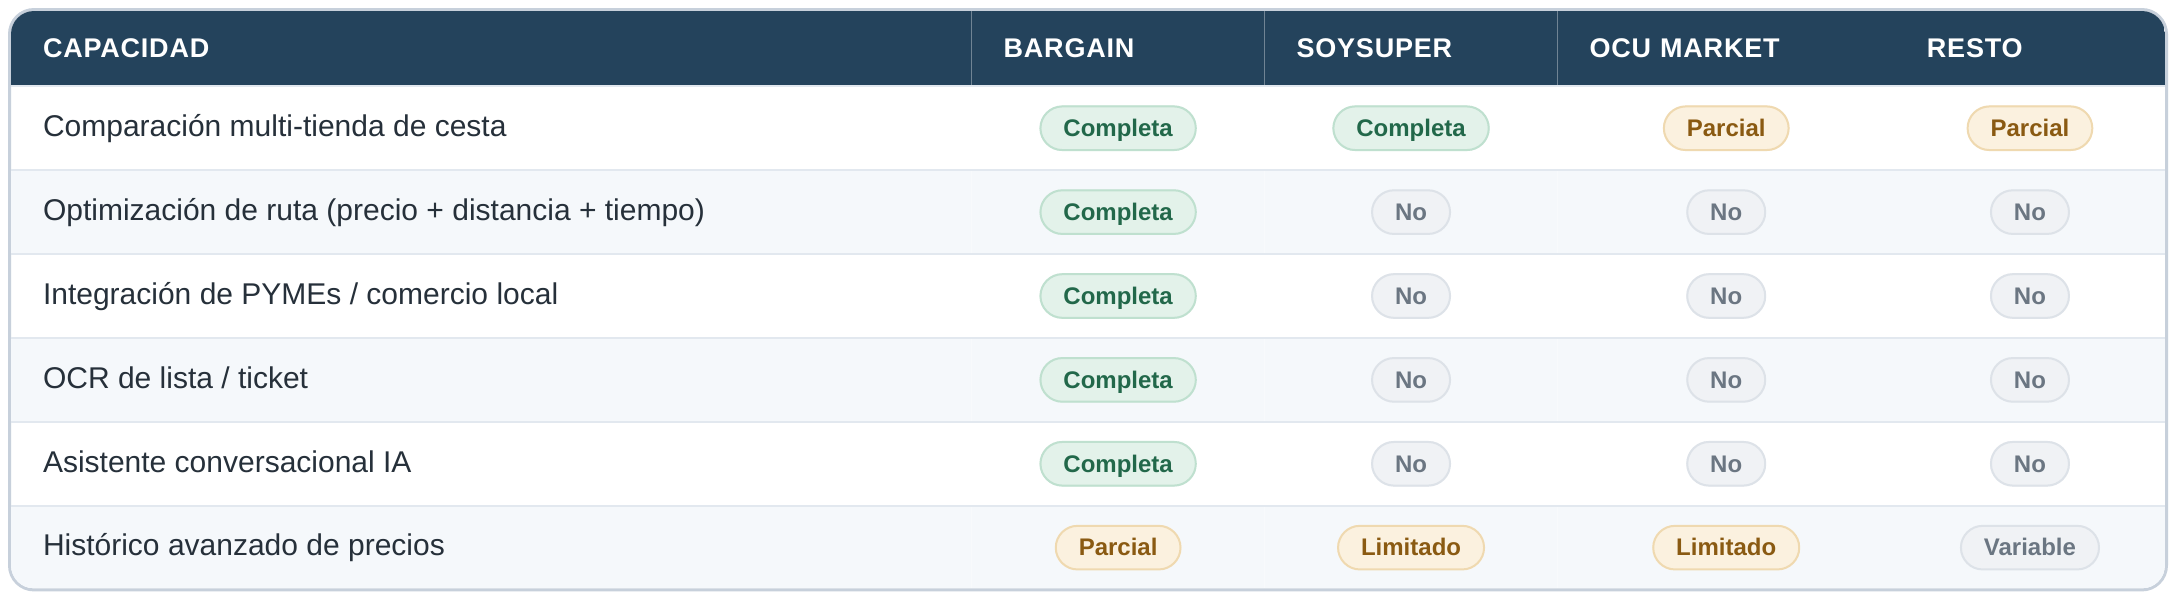
\includegraphics[width=0.95\textwidth]{diagramas/cuadros/cuadro-comparativa-alternativas.png}
\end{table}

\section{Brechas estrat\'egicas detectadas}

El an\'alisis identifica cuatro brechas de mercado que justifican la propuesta:

\begin{enumerate}
	\item \textbf{Gap precio-ruta:} los comparadores muestran precios, pero no optimizan
		desplazamiento y tiempo.
	\item \textbf{Comercio local invisible:} no existe cobertura estable de PYMEs en
		herramientas generalistas.
	\item \textbf{Fricci\'on de entrada:} la lista de compra sigue siendo manual en la mayor\'ia
		de soluciones.
	\item \textbf{Interacci\'on limitada:} predominan filtros y b\'usquedas r\'igidas frente a
		consultas en lenguaje natural.
\end{enumerate}

\section{Posicionamiento de BargAIn}

BargAIn se posiciona como un \emph{optimizador inteligente de compra} y no solo como
comparador. Su propuesta de valor combina ahorro econ\'omico, eficiencia log\'istica y
experiencia de usuario asistida por IA.

\section{Riesgos competitivos}

Los riesgos principales identificados son:

\begin{itemize}
	\item reacci\'on de competidores consolidados con mayor base de usuarios,
	\item dependencia de fuentes de datos de terceros para scraping,
	\item necesidad de mantener alta calidad de datos para sostener confianza.
\end{itemize}

Como mitigaci\'on, se adopta una estrategia de fuentes h\'ibridas de datos, modularidad
arquitect\'onica y pipeline de validaci\'on continua.

     \chapter{An\'alisis temporal y costes de desarrollo}\label{analtemporal}

\section{Planificaci\'on temporal}

La planificaci\'on de BargAIn se defini\'o con una dedicaci\'on planificada de 300 horas,
distribuidas en fases funcionales y t\'ecnicas, que se ampli\'o hasta 325 horas reales al
incorporar el cierre documental y la preparaci\'on de la defensa. El proyecto se ejecut\'o de
forma iterativa, manteniendo trazabilidad en \texttt{TASKS.md} y en el \'arbol
\texttt{.planning/}.

\begin{table}[h]
\centering
\caption{Resumen por fases del proyecto}
\label{tab:fases-temporales}
\begin{tabular}{|l|c|c|c|}
\hline
\textbf{Fase} & \textbf{Semanas} & \textbf{Horas est.} & \textbf{Estado} \\
\hline
F1 An\'alisis y dise\~no & S1--S3 & 45 & Completada \\
F2 Infraestructura base & S3--S5 & 30 & Completada \\
F3 Desarrollo core backend & S5--S12 & 95 & Completada \\
F4 Desarrollo frontend & S8--S16 & 70 & Completada \\
F5 IA, optimizador y scraping & S10--S17 & 35 & Completada \\
F6 Portal business y app m\'ovil & S15--S18 & 25 & Completada \\
F7 Pruebas, deploy y cierre & S18--S20 & 25 & Completada \\
\hline
\textbf{Total} & & \textbf{325} & \textbf{Cerrado} \\
\hline
\end{tabular}
\end{table}

\section{Metodolog\'ia de trabajo}

Se aplic\'o una metodolog\'ia incremental con ciclos cortos por fase:

\begin{itemize}
	\item definici\'on de alcance y criterios de aceptaci\'on,
	\item implementaci\'on por m\'odulos,
	\item validaci\'on automatizada (lint + tests),
	\item verificaci\'on funcional y documental,
	\item cierre de fase con artefactos de evidencia.
\end{itemize}

Este enfoque permiti\'o absorber cambios sin comprometer la estabilidad del sistema.

\section{Estimaci\'on de costes}

La estimaci\'on econ\'omica se realiz\'o mediante coste-hora por rol junior,
alineada con referencias del informe de perfiles TIC de la Junta de Andaluc\'ia (2018).

\begin{table}[h]
\centering
\caption{Coste estimado del desarrollo}
\label{tab:coste-estimado}
\begin{tabular}{|l|c|c|}
\hline
\textbf{Bloque} & \textbf{Horas} & \textbf{Coste (EUR)} \\
\hline
An\'alisis y dise\~no & 45 & 1.490,40 \\
Infraestructura & 30 & 861,60 \\
Backend + frontend & 165 & 4.738,80 \\
IA, optimizador y scraping & 35 & 1.005,20 \\
Portal business y app m\'ovil & 25 & 718,00 \\
Pruebas y despliegue & 25 & 594,25 \\
\hline
\textbf{Total} & \textbf{325} & \textbf{9.408,25} \\
\hline
\end{tabular}
\end{table}

Adicionalmente, el coste operativo en staging se mantuvo bajo durante el TFG
gracias al uso de planes gratuitos o de bajo consumo (Render, Sentry, GitHub Actions).

\section{Riesgos y mitigaciones}

Los riesgos operativos principales fueron:

\begin{itemize}
	\item \textbf{Cambios en fuentes de scraping:} mitigado con spiders modulares y
		fallback de crowdsourcing.
	\item \textbf{Dependencia de APIs externas:} mitigado con cach\'e y degradaci\'on controlada.
	\item \textbf{Carga de trabajo en fases finales:} mitigado con cierre incremental de
		entregables y automatizaci\'on de validaci\'on.
\end{itemize}

\section{Resultado de planificaci\'on}

La planificaci\'on permiti\'o completar el alcance funcional priorizado del TFG,
incluyendo arquitectura, implementaci\'on, pruebas y despliegue de staging,
manteniendo coherencia entre roadmap, requisitos y evidencias de verificaci\'on.

     \chapter{Analisis de requisitos}\label{requisitos}

\section{Actores del sistema}

El sistema define cuatro actores principales:

\begin{itemize}
	\item \textbf{Consumidor:} crea listas, compara precios, optimiza rutas, usa OCR
		y consulta al asistente.
	\item \textbf{Comercio/PYME:} gestiona precios y promociones desde el portal business.
	\item \textbf{Administrador:} verifica perfiles, modera datos y supervisa operacion.
	\item \textbf{Sistema automatizado:} tareas de scraping y mantenimiento en segundo plano.
\end{itemize}

\section{Requisitos de informacion}

El modelo de informacion se articula en doce bloques (RI-001 a RI-012), que cubren:

\begin{itemize}
	\item usuarios y preferencias de optimizacion,
	\item catalogo (productos, categorias, marcas),
	\item tiendas geolocalizadas y cadenas,
	\item precios actuales e historicos,
	\item listas de compra y resultados de optimizacion,
	\item perfiles business y promociones,
	\item sesiones OCR y conversaciones del asistente.
\end{itemize}

\section{Requisitos funcionales}

Se definieron 35 requisitos funcionales (RF-001 a RF-035) agrupados por dominios:

\begin{table}[h]
\centering
\caption{Agrupacion de requisitos funcionales}
\label{tab:rf-grupos}
\begin{tabular}{|l|c|l|}
\hline
\textbf{Dominio} & \textbf{IDs} & \textbf{Capacidad principal} \\
\hline
Autenticacion y perfil & RF-001..RF-005 & Registro, login JWT, preferencias \\
Catalogo de productos & RF-006..RF-010 & Busqueda, detalle, crowdsourcing \\
Tiendas y mapa & RF-011..RF-014 & Proximidad, detalle, favoritos \\
Precios & RF-015..RF-019 & Comparacion, historico, alertas \\
Listas de compra & RF-020..RF-023 & CRUD, compartir, plantillas \\
Optimizador & RF-024..RF-027 & Ruta multicriterio y recalculo \\
OCR & RF-028..RF-029 & Captura y matching fuzzy \\
Asistente LLM & RF-030..RF-031 & Consultas naturales y sugerencias \\
Portal business & RF-032..RF-034 & Onboarding, precios, promociones \\
Notificaciones & RF-035 & Push/email por eventos \\
\hline
\end{tabular}
\end{table}

\section{Criterios de aceptacion del producto}

Los criterios de aceptacion se validan a nivel funcional y de experiencia:

\begin{itemize}
	\item flujo de alta y acceso operativo en menos de 3 minutos,
	\item comparacion de cesta completa en entorno de tiendas cercanas,
	\item optimizacion con top-3 rutas y desglose por parada,
	\item OCR con confirmacion/edicion previa a insercion en lista,
	\item portal PYME con gestion de precios y promociones,
	\item notificaciones de eventos criticos (alertas, promociones, cambios compartidos).
\end{itemize}

\section{Requisitos no funcionales}

Se definieron ocho requisitos no funcionales (RNF-001 a RNF-008):

\begin{itemize}
	\item rendimiento API (p95 bajo para operaciones CRUD y optimizacion),
	\item disponibilidad de staging,
	\item seguridad (JWT, HTTPS, rate limiting),
	\item usabilidad (flujo principal corto y criterios de accesibilidad),
	\item escalabilidad arquitectonica,
	\item mantenibilidad con cobertura y convenciones,
	\item compatibilidad multiplataforma,
	\item cumplimiento RGPD.
\end{itemize}

\section{Reglas de negocio}

Las reglas RN-001..RN-010 gobiernan limites y politicas operativas:

\begin{itemize}
	\item radio maximo de busqueda y numero maximo de paradas,
	\item caducidad y prioridad de fuentes de precio,
	\item restricciones del asistente a dominio de compra,
	\item verificacion previa de perfiles business,
	\item politicas de scraping responsable y frecuencia de ejecucion.
\end{itemize}

\section{Diagramas de casos de uso}

Los diagramas de casos de uso recogen las interacciones principales de cada actor con el sistema.

\begin{figure}[htbp]
\centering

\includegraphics[width=0.85\textwidth]{../diagramas/casos-uso/casos-uso-consumidor.png}
\caption{Casos de uso del Consumidor}
\label{fig:casos-uso-consumidor}
\end{figure}

\begin{figure}[htbp]
\centering

\includegraphics[width=0.85\textwidth]{../diagramas/casos-uso/casos-uso-comercio-admin.png}
\caption{Casos de uso del Comercio y Administrador}
\label{fig:casos-uso-comercio}
\end{figure}

\section{Trazabilidad}

La trazabilidad entre requisitos, implementacion y pruebas se mantiene en:

\begin{itemize}
	\item \texttt{docs/memoria/07-requisitos.md} (especificacion completa),
	\item \texttt{TASKS.md} (estado por fase/tarea),
	\item \texttt{tests/unit}, \texttt{tests/integration} y \texttt{frontend/web/e2e}
		(verificacion ejecutable).
\end{itemize}

     % !TEX root = ../proyect.tex

\chapter{Dise\~no e Implementaci\'on}\label{cap08}

\section{Arquitectura del Sistema}\label{sec:arquitectura}

\subsection{Visi\'on general}\label{subsec:vision-general}

BargAIN sigue una arquitectura de \textbf{tres capas} cl\'asica (presentaci\'on, l\'ogica de
negocio y datos), desplegada mediante contenedores Docker y organizada internamente seg\'un los
principios de la \textbf{arquitectura hexagonal} (puertos y adaptadores). Esta elecci\'on permite
desacoplar la l\'ogica de dominio de los detalles de infraestructura --- bases de datos, APIs
externas, brokers de mensajer\'ia --- facilitando el testing independiente de cada componente.

La arquitectura global se divide en cinco bloques principales:

\begin{enumerate}
  \item \textbf{Aplicaci\'on cliente:} React Native (Expo) para iOS y Android, con una aplicaci\'on
    web React para el Portal Business de PYMEs.
  \item \textbf{API Backend:} Django REST Framework como n\'ucleo de la l\'ogica de negocio,
    expuesto bajo HTTPS mediante Gunicorn + Nginx.
  \item \textbf{Capa de datos:} PostgreSQL 16 con extensi\'on PostGIS 3.4 para consultas
    geoespaciales.
  \item \textbf{Capa de tareas as\'incronas:} Celery con Redis como broker, para scraping
    peri\'odico, env\'io de notificaciones, procesamiento OCR y c\'alculos del optimizador.
  \item \textbf{Integraciones y servicios auxiliares:} Google Gemini API (asistente LLM),
    OpenRouteService (c\'alculo de distancias reales), Google Cloud Vision API (OCR) y Sentry
    (monitorizaci\'on de errores).
\end{enumerate}

\subsection{Patr\'on de organizaci\'on interna del backend}\label{subsec:patron-backend}

Cada aplicaci\'on Django del backend sigue una estructura modular consistente:

\begin{verbatim}
apps/<modulo>/
|-- models.py          # Entidades de dominio (ORM)
|-- serializers.py     # Transformacion de datos (entrada/salida)
|-- views.py           # ViewSets y vistas (controladores)
|-- urls.py            # Rutas del modulo
|-- services.py        # Logica de negocio
|-- tasks.py           # Tareas Celery asincronas
|-- permissions.py     # Logica de autorizacion
`-- tests/
\end{verbatim}

La separaci\'on entre \texttt{views.py} y \texttt{services.py} es deliberada: los ViewSets se
limitan a la gesti\'on HTTP (autenticaci\'on, serializaci\'on, c\'odigos de respuesta), mientras
que la l\'ogica de negocio reside exclusivamente en los servicios, lo que permite invocarla desde
tareas Celery o tests sin simular peticiones HTTP.

La Figura~\ref{fig:arquitectura-capas} resume la distribuci\'on por capas de la soluci\'on.

\begin{figure}[htbp]
\centering

\includegraphics[width=0.92\textwidth]{../diagramas/arquitectura/arquitectura-capas.png}
\caption{Arquitectura por capas de BargAIN}
\label{fig:arquitectura-capas}
\end{figure}

\subsection{Comunicaci\'on entre componentes}\label{subsec:comunicacion}

\begin{itemize}
  \item \textbf{Frontend \textrightarrow{} Backend:} API REST con autenticaci\'on JWT. Axios
    gestiona la renovaci\'on autom\'atica del token de acceso ante un \texttt{401 Unauthorized}.
  \item \textbf{Backend \textrightarrow{} Celery:} Encolar tareas mediante \texttt{.delay()} o
    \texttt{.apply\_async()} sobre el broker Redis.
  \item \textbf{Backend \textrightarrow{} PostgreSQL:} Django ORM con consultas geoespaciales
    mediante \texttt{django.contrib.gis}.
  \item \textbf{Backend \textrightarrow{} APIs externas:} Clientes HTTP aislados en
    \texttt{apps/<modulo>/clients/} para Google Maps, Gemini API y ORS.
\end{itemize}

\section{Modelo de Datos}\label{sec:modelo-datos}

\subsection{M\'odulo de usuarios}\label{subsec:modelo-usuarios}

El modelo \texttt{User} extiende \texttt{AbstractBaseUser} de Django para permitir el login
mediante email. Se definen tres roles: \texttt{consumer}, \texttt{business} y \texttt{admin}.
El campo \texttt{default\_location} utiliza \texttt{PointField(SRID=4326)}.

Las preferencias de optimizaci\'on (\texttt{w\_precio}, \texttt{w\_distancia}, \texttt{w\_tiempo})
se almacenan como decimales con restricci\'on de que su suma sea igual a 1.0, validada a nivel de
serializer:

\begin{verbatim}
def validate(self, data: dict) -> dict:
    weights = [
        data.get('weight_price', 0),
        data.get('weight_distance', 0),
        data.get('weight_time', 0),
    ]
    if abs(sum(weights) - 1.0) > 0.001:
        raise serializers.ValidationError(
            "Los pesos de optimizacion deben sumar exactamente 1.0"
        )
    return data
\end{verbatim}

\subsection{M\'odulo de productos}\label{subsec:modelo-productos}

La b\'usqueda de productos por nombre utiliza \textbf{matching fuzzy} mediante la extensi\'on
PostgreSQL \texttt{pg\_trgm} (trigramas). El campo \texttt{normalized\_name} almacena el nombre
normalizado (min\'usculas, sin tildes, sin caracteres especiales) con \'indices GIN de trigramas:

\begin{verbatim}
def search_products(query: str, limit: int = 20) -> QuerySet[Product]:
    return (
        Product.objects
        .annotate(similarity=TrigramSimilarity(
            'normalized_name', normalize(query)))
        .filter(similarity__gt=0.3, is_active=True)
        .order_by('-similarity')[:limit]
    )
\end{verbatim}

\subsection{M\'odulo de tiendas}\label{subsec:modelo-tiendas}

El campo \texttt{location} de \texttt{Store} es un \texttt{PointField} con \'indice GiST para
b\'usquedas geoespaciales eficientes:

\begin{verbatim}
def get_stores_in_radius(
    lat: float, lng: float, radius_km: float
) -> QuerySet[Store]:
    user_location = Point(lng, lat, srid=4326)
    return (
        Store.objects
        .filter(
            location__dwithin=(user_location, D(km=radius_km)),
            is_active=True
        )
        .annotate(distance=Distance('location', user_location))
        .order_by('distance')
    )
\end{verbatim}

El uso de \texttt{ST\_DWithin} en lugar de \texttt{ST\_Distance} en el \texttt{WHERE} es
deliberado: \texttt{ST\_DWithin} puede aprovechar el \'indice GiST, mientras que calcular
distancias en el filtro forzar\'ia un escaneo completo de la tabla.

\subsection{M\'odulo de precios}\label{subsec:modelo-precios}

El hist\'orico de precios se materializa autom\'aticamente: cada precio es inmutable una vez
creado. La actualizaci\'on de un precio supone la inserci\'on de un nuevo registro. Una tarea
Celery peri\'odica (\texttt{expire\_stale\_prices}) marca como expirados los precios de scraping
con m\'as de 48 horas de antig\"uedad y los de crowdsourcing con m\'as de 24 horas.

\subsection{M\'odulo del optimizador}\label{subsec:modelo-optimizador}

El m\'odulo del optimizador incluye tres entidades relacionales para almacenar el resultado de la
optimizaci\'on de forma trazable:

\begin{itemize}
  \item \textbf{\texttt{OptimizationResult}:} resultado global con pesos, modo y m\'etricas
    totales. Incluye \texttt{route\_data} JSONB para compatibilidad de lectura r\'apida.
  \item \textbf{\texttt{OptimizationRouteStop}:} cada parada de la ruta con tienda, orden,
    distancia, tiempo y subtotal.
  \item \textbf{\texttt{OptimizationRouteStopItem}:} \'item concreto por parada, con producto
    resuelto, precio elegido, texto original y puntuaci\'on de similitud.
\end{itemize}

\subsection{\'Indices clave}\label{subsec:indices}

\begin{table}[h]
\caption{\'Indices principales de la base de datos}
\label{tab:indices}
\centering
\begin{tabular}{|l|l|l|p{5cm}|}
\hline
\textbf{Tabla} & \textbf{Columna(s)} & \textbf{Tipo} & \textbf{Justificaci\'on} \\
\hline
\texttt{store} & \texttt{location} & GiST &
  B\'usquedas geoespaciales por radio \\
\texttt{price} & \texttt{(product, store, created\_at)} & B-Tree &
  Hist\'orico y precio actual \\
\texttt{price} & \texttt{expires\_at} & B-Tree parcial &
  Filtrar precios vigentes \\
\texttt{product} & \texttt{normalized\_name} & GIN (trigram) &
  B\'usqueda fuzzy por nombre \\
\texttt{shopping\_list\_item} & \texttt{(shopping\_list, is\_checked)} & B-Tree &
  \'Items pendientes \\
\hline
\end{tabular}
\end{table}

\subsection{Modelo entidad-relaci\'on}\label{subsec:modelo-er}

La Figura~\ref{fig:modelo-er} muestra el diagrama entidad-relaci\'on completo de la base de datos.

\begin{figure}[htbp]
\centering

\includegraphics[width=\textwidth]{../diagramas/er/modelo-er.png}
\caption{Diagrama entidad-relaci\'on de BargAIN}
\label{fig:modelo-er}
\end{figure}

\subsection{Diagrama de clases}\label{subsec:modelo-clases}

La Figura~\ref{fig:modelo-clases} detalla las clases principales del dominio y sus relaciones.

\begin{figure}[htbp]
\centering

\includegraphics[width=\textwidth]{../diagramas/clases/modelo-clases.png}
\caption{Diagrama de clases del dominio}
\label{fig:modelo-clases}
\end{figure}

\section{Dise\~no de la API REST}\label{sec:api}

\subsection{Estructura general}\label{subsec:api-estructura}

La API sigue las convenciones REST y est\'a versionada bajo el prefijo \texttt{/api/v1/}. Todos
los endpoints requieren autenticaci\'on JWT salvo los de registro y login. Las respuestas siguen
el formato unificado:

\begin{verbatim}
// Respuesta exitosa
{
  "success": true,
  "data": { ... },
  "meta": { "count": 42, "page": 1, "page_size": 20 }
}

// Respuesta de error
{
  "success": false,
  "error": {
    "code": "STORE_NOT_FOUND",
    "message": "No se encontraron tiendas en el radio especificado",
    "details": {}
  }
}
\end{verbatim}

\subsection{Endpoints principales}\label{subsec:api-endpoints}

\begin{table}[h]
\caption{Endpoints de autenticaci\'on y usuarios}
\label{tab:api-auth}
\centering
\begin{tabular}{|l|p{6cm}|p{5cm}|}
\hline
\textbf{M\'etodo} & \textbf{Endpoint} & \textbf{Descripci\'on} \\
\hline
\texttt{POST} & \texttt{/api/v1/auth/register/} & Registro de nuevo usuario \\
\texttt{POST} & \texttt{/api/v1/auth/login/} & Login: access + refresh token \\
\texttt{POST} & \texttt{/api/v1/auth/token/refresh/} & Renovar access token \\
\texttt{POST} & \texttt{/api/v1/auth/logout/} & Invalidar refresh token \\
\texttt{GET/PATCH} & \texttt{/api/v1/users/me/} & Perfil del usuario autenticado \\
\texttt{GET/PATCH} & \texttt{/api/v1/users/me/preferences/} & Preferencias de optimizaci\'on \\
\hline
\end{tabular}
\end{table}

\begin{table}[h]
\caption{Endpoints del optimizador, OCR y asistente}
\label{tab:api-core}
\centering
\begin{tabular}{|l|p{6cm}|p{5cm}|}
\hline
\textbf{M\'etodo} & \textbf{Endpoint} & \textbf{Descripci\'on} \\
\hline
\texttt{POST} & \texttt{/api/v1/optimize/} & Calcular o recalcular ruta \'optima \\
\texttt{GET} & \texttt{/api/v1/optimize/?shopping\_list\_id=\{id\}} &
  Cargar \'ultima ruta persistida \\
\texttt{POST} & \texttt{/api/v1/ocr/scan/} &
  Procesar imagen y devolver \'items reconocidos \\
\texttt{GET/POST} & \texttt{/api/v1/assistant/conversations/} &
  Listar y crear conversaciones \\
\texttt{POST} & \texttt{/api/v1/assistant/conversations/\{id\}/messages/} &
  Enviar mensaje al asistente \\
\hline
\end{tabular}
\end{table}

\subsection{Autenticaci\'on y autorizaci\'on}\label{subsec:api-auth}

Se implementa un sistema de permisos a tres niveles:

\begin{itemize}
  \item \textbf{\texttt{IsAuthenticated}:} Aplicado por defecto a todos los endpoints privados.
  \item \textbf{\texttt{IsBusinessOwner}:} Permite operar solo sobre el perfil de negocio propio.
  \item \textbf{\texttt{IsAdminUser}:} Para endpoints de administraci\'on del sistema.
  \item \textbf{\texttt{IsShoppingListOwnerOrShared}:} Permite acceso al propietario y
    colaboradores invitados.
\end{itemize}

Los tokens JWT se generan con \texttt{djangorestframework-simplejwt}. El token de acceso tiene
validez de 60 minutos y el de refresco de 7 d\'ias con rotaci\'on autom\'atica.

\section{Implementaci\'on del Backend}\label{sec:implementacion-backend}

\subsection{M\'odulo de notificaciones}\label{subsec:impl-notificaciones}

El m\'odulo gestiona el buz\'on de notificaciones del usuario (inbox) y el env\'io de
notificaciones push mediante \textbf{Expo Push Notifications}. Las entregas se procesan
as\'incronamente con tareas Celery.

\begin{itemize}
  \item \textbf{\texttt{Notification}:} Registro persistente con \texttt{notification\_type}
    (\texttt{price\_alert}, \texttt{new\_promo}, \texttt{shared\_list\_changed},
    \texttt{business\_approved}, \texttt{business\_rejected}), campos \texttt{title}/\texttt{body},
    bandera \texttt{is\_read}, \texttt{data} JSONB para payload variable, \texttt{action\_url}
    para deep links y \texttt{deleted\_at} para soft-delete.
  \item \textbf{\texttt{UserPushToken}:} Token Expo registrado por dispositivo. La clave \'unica
    \texttt{(user, device\_id)} evita duplicados al reinstalar la app.
\end{itemize}

\subsection{M\'odulo de portal business}\label{subsec:impl-business}

\begin{itemize}
  \item \textbf{\texttt{BusinessProfile}:} Perfil verificable con \texttt{tax\_id} (CIF/NIF
    \'unico), estado de verificaci\'on y umbral de alerta de competidor
    (\texttt{price\_alert\_threshold\_pct}).
  \item \textbf{\texttt{Promotion}:} Promoci\'on temporal de un producto en una tienda. Restricci\'on
    parcial \'unica \texttt{(product, store) WHERE is\_active} garantiza que no existan dos
    promociones activas para el mismo par.
\end{itemize}

La tarea Celery \texttt{check\_competitor\_prices} se ejecuta cada 6 horas y alerta al propietario
cuando detecta diferencias superiores al umbral configurado.

\section{El Algoritmo de Optimizaci\'on de Rutas}\label{sec:algoritmo}

\subsection{Formulaci\'on del problema}\label{subsec:formulacion}

El algoritmo de optimizaci\'on es la aportaci\'on t\'ecnica central del TFG. El problema es una
variante del \textbf{Vehicle Routing Problem (VRP)} con objetivos m\'ultiples, resuelto mediante
una soluci\'on heur\'istica eficiente.

\textbf{Entrada:}
\begin{itemize}
  \item Lista de la compra $L = \{i_1, i_2, \ldots, i_n\}$ (n \'items textuales)
  \item Ubicaci\'on del usuario $u = (lat, lng)$
  \item Radio m\'aximo $r$ (km), n\'umero m\'aximo de paradas $k$ (1--4)
  \item Pesos de preferencia $w_{precio}$, $w_{distancia}$, $w_{tiempo}$ (suman 1.0)
\end{itemize}

\textbf{Salida:} Top-3 asignaciones de \'items resueltos a tiendas que minimizan la funci\'on
de coste.

\subsection{Funci\'on de scoring multicriterio}\label{subsec:scoring}

\begin{equation}
  \text{Score}(A) = w_{precio} \cdot \text{ahorro\_norm}(A)
                 - w_{distancia} \cdot \text{dist\_extra\_norm}(A)
                 - w_{tiempo} \cdot \text{tiempo\_extra\_norm}(A)
\end{equation}

Donde \texttt{ahorro\_normalizado} = $(\text{coste\_single\_best} - \text{coste}(A)) /
\text{coste\_single\_best} \in [0, 1]$ y \texttt{distancia\_extra\_normalizada} = $\max(0,
\text{dist\_ruta}(A) - \text{dist\_single}) / (r \times 1{,}5)$.

\subsection{Pipeline de ejecuci\'on}\label{subsec:pipeline}

El algoritmo se ejecuta en seis fases secuenciales dentro de
\texttt{apps/optimizer/services.py}:

\begin{enumerate}
  \item \textbf{Fase 0 --- Resoluci\'on textual de \'items:} Preseleccion por trigramas sobre
    \texttt{Product.normalized\_name}, ranking fuzzy (\texttt{token\_set\_ratio}), y validaci\'on
    contextual por disponibilidad de precio.

  \item \textbf{Fase 1 --- Ingesta de precios candidatos:} Para cada producto resuelto, se
    obtienen los precios vigentes en tiendas dentro del radio con una sola consulta optimizada
    con \texttt{select\_related} y filtros geoespaciales.

  \item \textbf{Fase 2 --- Pre-filtrado de tiendas:} Se limita a 30 tiendas candidatas m\'aximo
    para controlar la explosi\'on combinatoria (C(30, 3) = 4.060 combinaciones para k=3).

  \item \textbf{Fase 3 --- Generaci\'on y evaluaci\'on de asignaciones:} Para cada combinaci\'on
    de tiendas, asignaci\'on greedy \'optima de \'items al menor precio disponible.

  \item \textbf{Fase 4 --- C\'alculo de distancias reales:} Matriz de distancias v\'ia
    \textbf{OpenRouteService (ORS)} en una sola petici\'on. Fallback haversine si ORS no est\'a
    disponible:

\begin{verbatim}
POST https://api.openrouteservice.org/v2/matrix/driving-car
Authorization: {ORS_API_KEY}

{
  "locations": [[lng1, lat1], [lng2, lat2], ...],
  "metrics": ["distance", "duration"],
  "units": "km"
}
\end{verbatim}

  \item \textbf{Fase 5 --- Scoring y ranking:} Normalizaci\'on de valores al rango [0, 1] y
    devoluci\'on de las top-3 asignaciones ordenadas por score descendente.
\end{enumerate}

\subsection{Diagrama de secuencia del optimizador}\label{subsec:secuencia-optimizador}

La Figura~\ref{fig:secuencia-optimizacion} ilustra el flujo de mensajes entre componentes
durante una petici\'on de optimizaci\'on.

\begin{figure}[htbp]
\centering

\includegraphics[width=0.95\textwidth]{../diagramas/secuencia/secuencia-optimizacion.png}
\caption{Diagrama de secuencia del proceso de optimizaci\'on de ruta}
\label{fig:secuencia-optimizacion}
\end{figure}

\subsection{Integraci\'on con OR-Tools}\label{subsec:ortools}

Para combinaciones complejas donde el problema de asignaci\'on supera la heur\'istica greedy, se
utiliza \textbf{OR-Tools de Google} para resolver el problema como programaci\'on lineal entera
(ILP), garantizando la optimalidad de la asignaci\'on de productos a tiendas dentro de un
subconjunto fijo de tiendas.

\subsection{Complejidad y rendimiento}\label{subsec:rendimiento}

\begin{table}[h]
\caption{Tiempos estimados de ejecuci\'on del optimizador}
\label{tab:rendimiento}
\centering
\begin{tabular}{|l|c|c|c|}
\hline
\textbf{Escenario} & \textbf{Tiendas} & \textbf{Combinaciones (k=3)} & \textbf{Tiempo} \\
\hline
Lista peque\~na (5 prod.) & $\leq 15$ & 455 & $<$ 1 s \\
Lista media (20 prod.) & $\leq 30$ & 4.060 & $<$ 3 s \\
Lista grande (50 prod.) & $\leq 30$ & 4.060 & $<$ 5 s \\
\hline
\end{tabular}
\end{table}

El umbral de 5 s (RNF-001) se cumple gracias a: pre-filtrado de tiendas, cach\'e de matriz de
distancias en Redis, y ejecuci\'on como tarea Celery as\'incrona.

\section{M\'odulo de Web Scraping}\label{sec:scraping}

El scraper es un \textbf{proyecto Scrapy independiente} (\texttt{scraping/}) desacoplado del
backend Django, que comunica con la base de datos a trav\'es de la API REST del propio backend.

Cada cadena requiere una estrategia diferente:

\begin{itemize}
  \item \textbf{Mercadona:} API interna (\texttt{uapi.mercadona.es}) no oficial pero estable,
    accesible mediante peticiones HTTP est\'andar.
  \item \textbf{Carrefour / Lidl / DIA:} Cat\'alogos con renderizado del lado del cliente (SPA),
    por lo que se usa \textbf{Playwright} para ejecutar el JavaScript y obtener el DOM hidratado.
\end{itemize}

Los spiders se programan con \textbf{Celery Beat}, con un delay m\'inimo de 2 segundos entre
peticiones consecutivas (regla de negocio RN-010).

\section{M\'odulo OCR}\label{sec:ocr}

El backend invoca \textbf{Google Cloud Vision API} con la imagen capturada por el usuario. La
decisi\'on de migrar desde Tesseract a Vision API se adopt\'o tras comprobar que Tesseract no
reconoce con suficiente claridad tickets y listas fotografiadas en condiciones reales:

\begin{verbatim}
from google.cloud import vision

def extract_text_from_image(image_bytes: bytes) -> list[str]:
    """Extrae lineas de texto mediante Google Cloud Vision API."""
    client = vision.ImageAnnotatorClient()
    image = vision.Image(content=image_bytes)
    response = client.text_detection(image=image)
    full_text = response.full_text_annotation.text
    return [line.strip() for line in full_text.splitlines() if line.strip()]
\end{verbatim}

Cada l\'inea extra\'ida se normaliza y se busca en el cat\'alogo mediante el servicio de matching
fuzzy de \texttt{apps/products}. Se devuelve una lista de candidatos con nivel de confianza.

\subsection{Diagrama de secuencia OCR}\label{subsec:secuencia-ocr}

La Figura~\ref{fig:secuencia-ocr} muestra el flujo de procesamiento desde la captura de imagen
hasta la inserci\'on de \'items en la lista.

\begin{figure}[htbp]
\centering

\includegraphics[width=0.95\textwidth]{../diagramas/secuencia/secuencia-ocr.png}
\caption{Diagrama de secuencia del flujo OCR}
\label{fig:secuencia-ocr}
\end{figure}

\section{Integraci\'on del Asistente LLM}\label{sec:asistente}

El asistente conversacional utiliza la \textbf{Google Gemini API}
(\texttt{gemini-2.0-flash-lite}) como modelo subyacente (ADR-008). El backend actúa como proxy,
añadiendo contexto de la compra del usuario al system prompt antes de enviar cada mensaje a la
API mediante el SDK \texttt{google-genai}.

Se aplica una \textbf{ventana deslizante} sobre el historial de mensajes (\'ultimos 20 mensajes
+ system prompt) para mantener el consumo de tokens controlado. El system prompt incluye un
guardrail que limita las respuestas a consultas de compra dom\'estica (RN-007).

\section{Infraestructura y Despliegue}\label{sec:infraestructura}

\subsection{Contenedores Docker}\label{subsec:docker}

Cada componente se ejecuta en un contenedor independiente, orquestados con Docker Compose:

\begin{itemize}
  \item \textbf{nginx:} Reverse proxy y servicio de est\'aticos.
  \item \textbf{backend:} Django + Gunicorn (3 workers).
  \item \textbf{celery-worker:} Workers para tareas as\'incronas.
  \item \textbf{celery-beat:} Scheduler de tareas peri\'odicas.
  \item \textbf{db:} PostgreSQL 16 + PostGIS.
  \item \textbf{redis:} Broker Celery + cach\'e.
\end{itemize}

Para el entorno de desarrollo se usa el modelo h\'ibrido (ADR-002): backend en Docker, frontend
nativo en el host. Docker volumes en Windows rompen el HMR de Metro/Expo, por lo que el frontend
no se dockeriza.

\subsection{Pipeline CI/CD}\label{subsec:cicd}

El repositorio incluye tres workflows de GitHub Actions:

\begin{itemize}
  \item \textbf{\texttt{ci-backend.yml}:} Ejecuta \texttt{ruff check}, \texttt{ruff format
    --check} y \texttt{pytest --cov} en cada push a cualquier rama.
  \item \textbf{\texttt{ci-frontend.yml}:} Ejecuta \texttt{eslint}, \texttt{prettier --check}
    y \texttt{jest --coverage} en cada push.
  \item \textbf{\texttt{ios-build.yml}:} Genera el \texttt{.ipa} unsigned mediante
    \texttt{expo prebuild} + \texttt{xcodebuild} en un runner \texttt{macos-latest}. El artefacto
    se descarga y se instala en el iPhone de demo con Sideloadly.
\end{itemize}

El deploy a staging se realiza mediante \textbf{Render Blueprints} (\texttt{render.yaml} en la
ra\'iz del repositorio), que define declarativamente 5 servicios. Cada push a \texttt{main}
dispara un redespliegue autom\'atico.

\subsection{Variables de entorno}\label{subsec:env}

La configuraci\'on sensible (claves API, credenciales de BD, secret key de Django) se gestiona
exclusivamente mediante variables de entorno, nunca hardcodeadas. Se proporciona
\texttt{.env.example} con los nombres de todas las variables requeridas.

\section{Dise\~no de la Interfaz de Usuario}\label{sec:ui}

\subsection{Sistema de dise\~no}\label{subsec:design-system}

El frontend define un sistema de dise\~no propio en \texttt{src/theme/} con los siguientes
tokens:

\begin{table}[h]
\caption{Paleta de colores del sistema de dise\~no}
\label{tab:colores}
\centering
\begin{tabular}{|l|l|l|}
\hline
\textbf{Token} & \textbf{Valor} & \textbf{Uso} \\
\hline
\texttt{primary} & \texttt{\#2E7D32} & Acciones principales, CTAs \\
\texttt{primaryLight} & \texttt{\#60AD5E} & Estados hover, fondos sutiles \\
\texttt{secondary} & \texttt{\#FF6F00} & Ahorros, destacados, ofertas \\
\texttt{surface} & \texttt{\#FAFAFA} & Fondo de tarjetas \\
\texttt{error} & \texttt{\#C62828} & Errores y alertas \\
\texttt{textPrimary} & \texttt{\#212121} & Texto principal \\
\texttt{textSecondary} & \texttt{\#757575} & Texto de apoyo \\
\hline
\end{tabular}
\end{table}

\textbf{Tipograf\'ia:} Inter (sans-serif) con escala modular. \textbf{Espaciado:} Escala de 4px.

\subsection{Pantallas principales}\label{subsec:pantallas}

La aplicaci\'on se estructura en cinco pesta\~nas principales:

\begin{enumerate}
  \item \textbf{Inicio / Dashboard:} Resumen de la lista activa, precio estimado en la tienda
    m\'as barata cercana, acceso r\'apido al asistente y alertas activas.
  \item \textbf{Mi Lista:} Gesti\'on de la lista activa con buscador de autocompletado, grupos
    por categor\'ia, swipe-to-delete/check y bot\'on de optimizar ruta.
  \item \textbf{Explorar:} Mapa interactivo con marcadores de tiendas y panel inferior
    deslizable con detalles de la tienda seleccionada.
  \item \textbf{Optimizador:} Sliders de pesos, cards comparativas de las top-3 rutas y
    visualizaci\'on de la ruta en mapa con polylines y marcadores numerados.
  \item \textbf{Perfil:} Datos personales, preferencias de optimizaci\'on, configuraci\'on de
    notificaciones y acceso al historial del asistente.
\end{enumerate}

     % !TEX root = ../proyect.tex

\chapter{Manual de Usuario}\label{cap09}

\section{Introducci\'on}\label{sec:manual-intro}

BargAIn permite al usuario gestionar su compra diaria desde una app m\'ovil (iOS y Android) y un
portal web para PYMEs, comparar precios entre supermercados cercanos, y calcular la ruta de compra
m\'as eficiente seg\'un sus preferencias de precio, distancia y tiempo.

\section{Requisitos de uso}\label{sec:manual-requisitos}

\begin{itemize}
  \item Dispositivo m\'ovil iOS (14+) o Android (10+) con la app instalada, o navegador web
    moderno para el portal business.
  \item Conexi\'on a Internet.
  \item Cuenta de usuario registrada en el sistema.
  \item Permisos de ubicaci\'on concedidos a la app (para funciones de mapa y optimizaci\'on).
\end{itemize}

Para el entorno de desarrollo local:
\begin{itemize}
  \item Backend levantado en Docker (\texttt{make dev}).
  \item Base de datos migrada (\texttt{make migrate-docker}).
  \item Frontend Expo en host (\texttt{make frontend}).
\end{itemize}

\section{Flujo de acceso}\label{sec:manual-acceso}

\begin{enumerate}
  \item Abrir la app en Expo/Web.
  \item Seleccionar ``Iniciar sesi\'on'' o ``Registrarse''.
  \item Introducir credenciales v\'alidas.
  \item Tras autenticaci\'on, se carga la navegaci\'on principal por pesta\~nas.
\end{enumerate}

El sistema usa JWT con refresco autom\'atico. Si el access token expira, la sesi\'on se recupera
sin intervenci\'on del usuario cuando el refresh token sigue siendo v\'alido (7 d\'ias desde el
\'ultimo uso).

\subsection{Pantallas de acceso}\label{subsec:manual-acceso-screens}

\begin{figure}[htbp]
\centering
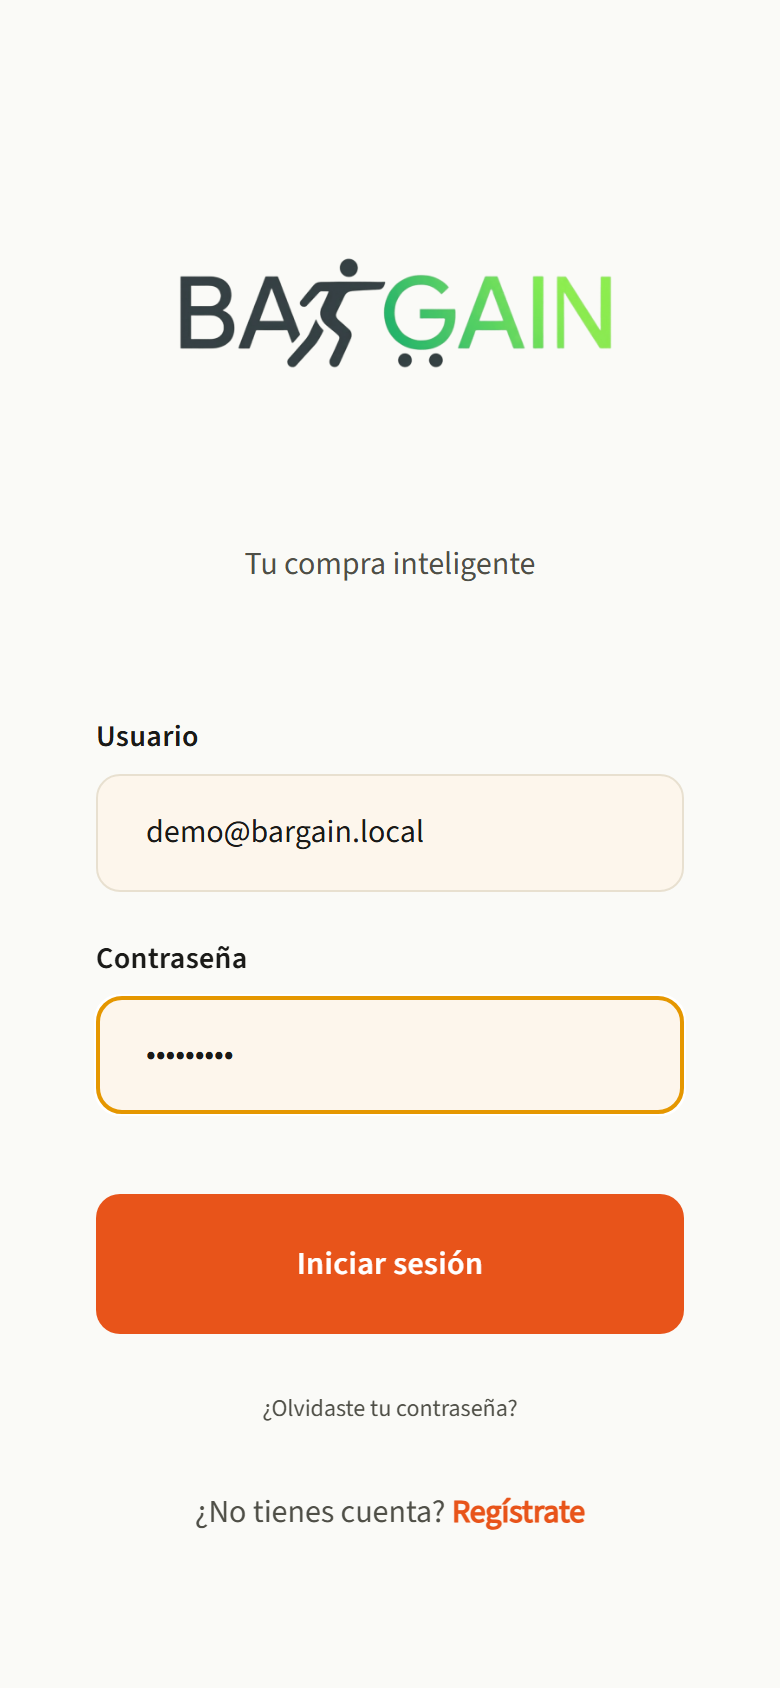
\includegraphics[width=0.32\textwidth]{diagramas/capturas/mobile-login.png}
\hfill
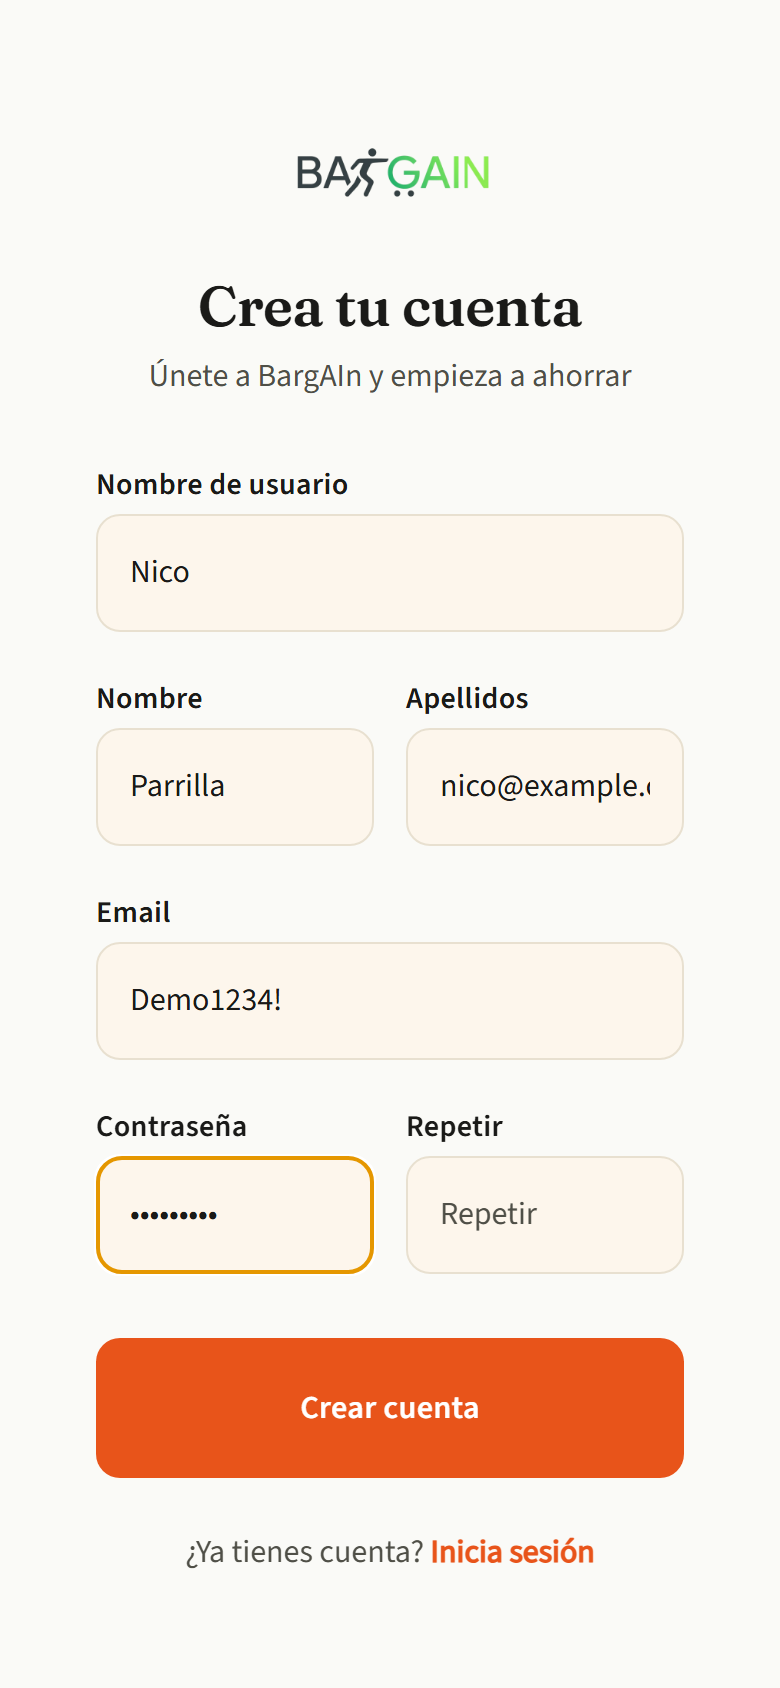
\includegraphics[width=0.32\textwidth]{diagramas/capturas/mobile-registro.png}
\caption{Pantallas de inicio de sesi\'on y registro}
\label{fig:ui-acceso}
\end{figure}

\section{Pantalla principal (Home)}\label{sec:manual-home}

La pantalla de inicio centraliza la informaci\'on m\'as relevante del usuario:

\begin{itemize}
  \item Resumen de listas activas con el precio estimado en la tienda m\'as barata cercana.
  \item CTA para crear lista cuando el usuario no tiene listas activas.
  \item Buscador global para navegar r\'apidamente a catálogo o funciones de compra.
  \item Acceso directo al asistente y a las alertas de precio activas.
\end{itemize}

\begin{figure}[htbp]
\centering
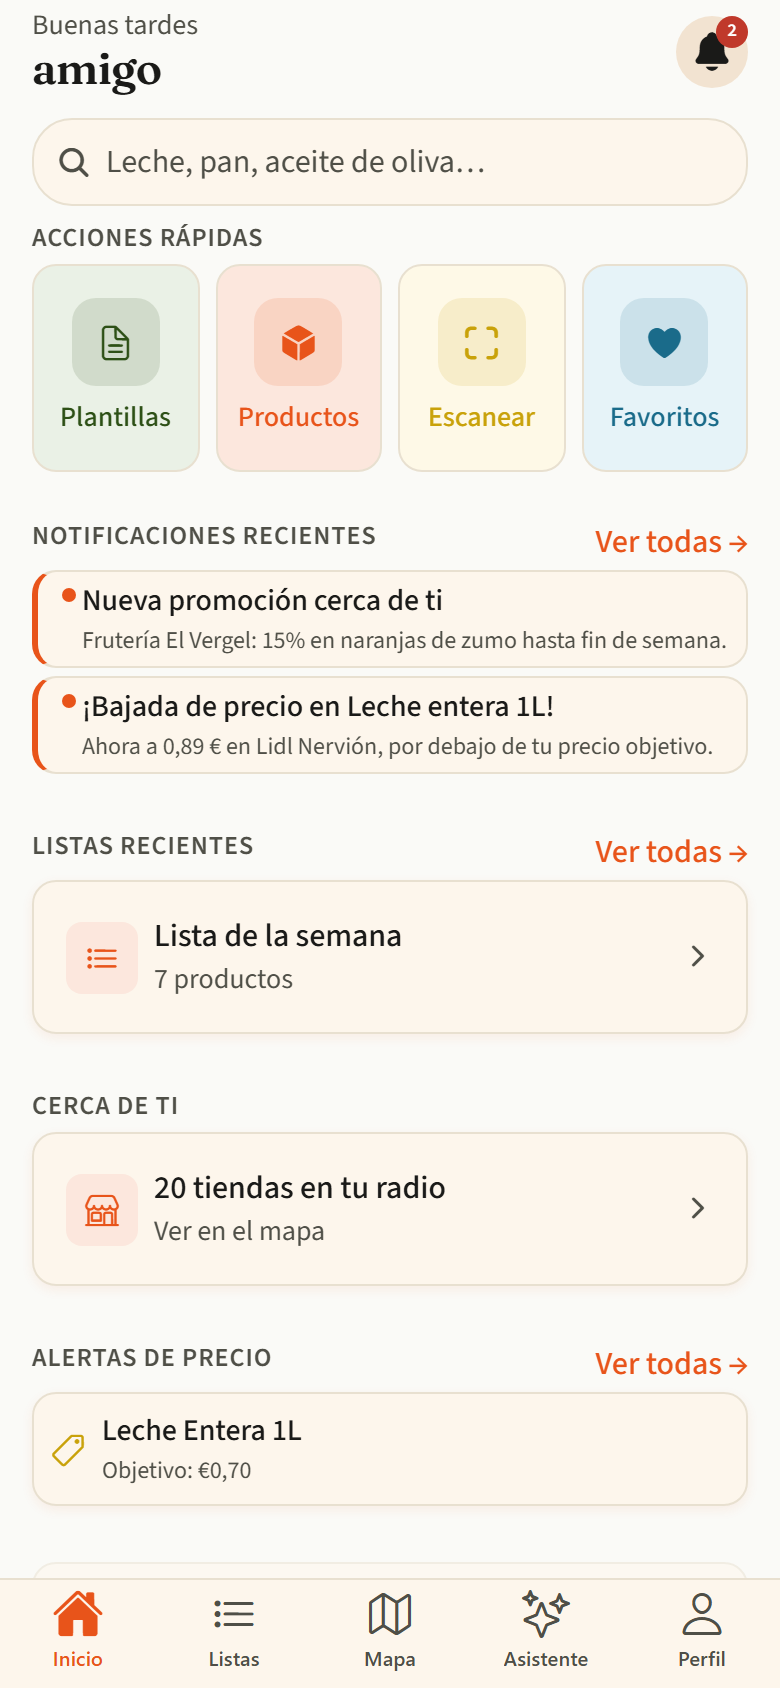
\includegraphics[width=0.40\textwidth]{diagramas/capturas/mobile-home.png}
\caption{Pantalla principal --- Dashboard}
\label{fig:ui-dashboard}
\end{figure}

\section{Gesti\'on de listas de compra}\label{sec:manual-listas}

\begin{enumerate}
  \item Crear lista con nombre personalizado (pesta\~na ``Mi Lista'' \textrightarrow{}
    bot\'on ``Nueva lista'').
  \item Abrir detalle de lista para ver \'items agrupados por categor\'ia.
  \item A\~nadir productos desde cat\'alogo o buscador con autocompletado.
  \item Ajustar cantidades con controles r\'apidos ``$+$/$-$''.
  \item Marcar productos como comprados (swipe-to-check) o eliminarlos (swipe-to-delete).
  \item Renombrar listas o convertirlas en plantilla para reutilizaci\'on futura.
  \item Compartir lista con colaboradores (hasta 10 usuarios por lista).
  \item Abrir ``Ruta optimizada'' para calcular, guardar y reutilizar la \'ultima ruta por lista.
\end{enumerate}

\begin{figure}[htbp]
\centering
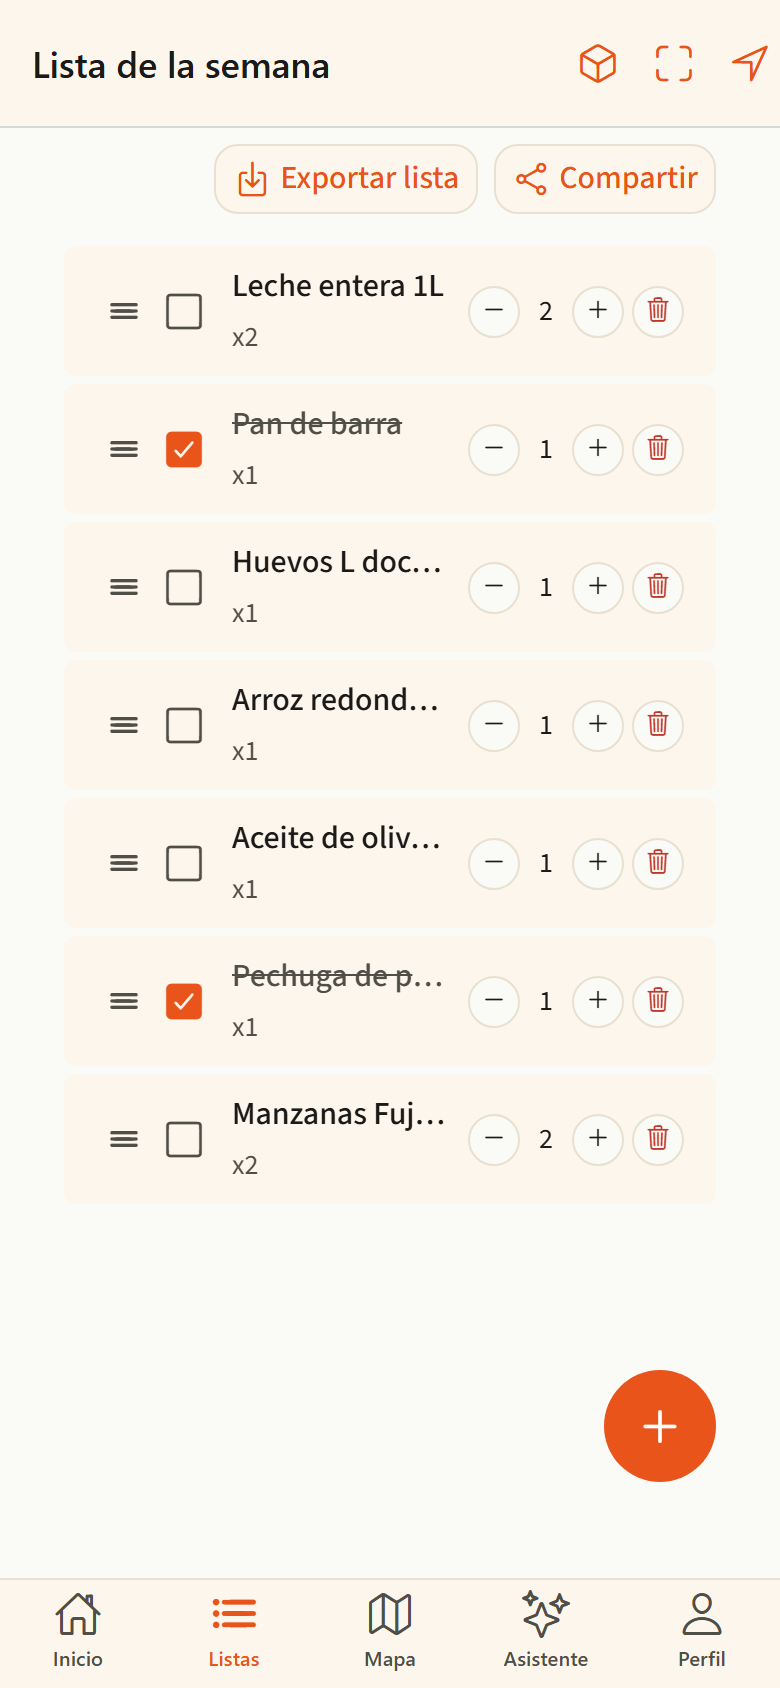
\includegraphics[width=0.40\textwidth]{diagramas/capturas/mobile-lista-detalle.png}
\caption{Pantalla de gesti\'on de lista de compra}
\label{fig:ui-lista}
\end{figure}

\section{Cat\'alogo y detalle de producto}\label{sec:manual-catalogo}

\begin{itemize}
  \item Cat\'alogo paginado con filtros plegables por categor\'ia, precio y distancia.
  \item Tarjetas de producto con precio m\'inimo detectado y nombre de la tienda m\'as barata.
  \item Acci\'on de a\~nadido r\'apido a lista desde la tarjeta (un tap).
  \item Detalle de producto con comparaci\'on de precios por tienda (tabla ordenable).
  \item Hist\'orico de precios con gr\'afico de evoluci\'on temporal.
\end{itemize}

\section{Mapa de tiendas}\label{sec:manual-mapa}

\begin{itemize}
  \item Visualizaci\'on de tiendas cercanas sobre mapa interactivo (React Native Maps).
  \item Marcadores diferenciados por cadena con badge de precio m\'inimo de la lista activa.
  \item Panel de tiendas plegable con detalles de la tienda seleccionada.
  \item Apertura de perfil de tienda desde el mapa y desde la lista de favoritas.
  \item Gesti\'on de tiendas favoritas (guardar, eliminar, acceder r\'apido).
\end{itemize}

\section{Alertas y notificaciones}\label{sec:manual-notificaciones}

\begin{itemize}
  \item Creaci\'on de alertas de precio: al abrir el detalle de un producto, pulsar ``Crear
    alerta'' e introducir el precio objetivo.
  \item Edici\'on y eliminaci\'on de alertas existentes desde la pantalla ``Mis alertas''.
  \item Bandeja de notificaciones con marcado como le\'ido individual o masivo y borrado
    funcional (soft-delete).
  \item Notificaciones push en el dispositivo para alertas de precio, nuevas promociones y
    cambios en listas compartidas.
\end{itemize}

\section{Perfil y preferencias}\label{sec:manual-perfil}

El usuario puede desde la pesta\~na ``Perfil'':

\begin{itemize}
  \item Editar datos b\'asicos (nombre, foto de avatar, tel\'efono).
  \item Ajustar preferencias del optimizador: radio de b\'usqueda (1--20 km), pesos
    $w_{precio}$/$w_{distancia}$/$w_{tiempo}$ (sliders que suman 1.0) y modo de
    optimizaci\'on (precio / distancia / balanced).
  \item Configurar preferencias de notificaciones (push, email, tipos de alerta).
  \item Cerrar sesi\'on (invalida el refresh token).
\end{itemize}

\section{Ruta optimizada persistente y rec\'alculo}\label{sec:manual-ruta}

Flujo recomendado:

\begin{enumerate}
  \item Entrar en una lista y pulsar ``Ruta optimizada''.
  \item Si existe una ruta previa para esa lista, se carga autom\'aticamente desde base de datos.
  \item Revisar paradas, productos por parada y precio total estimado.
  \item Pulsar ``Recalcular ruta'' para lanzar una nueva optimizaci\'on con ubicaci\'on y pesos
    actuales.
  \item Pulsar ``Ver en mapa'' para abrir la ruta circular en la app de mapas del dispositivo.
\end{enumerate}

Comportamiento persistente: la app no pierde la ruta al salir de la pantalla. Al volver, recupera
la \'ultima optimizaci\'on guardada de esa lista.

\begin{figure}[htbp]
\centering
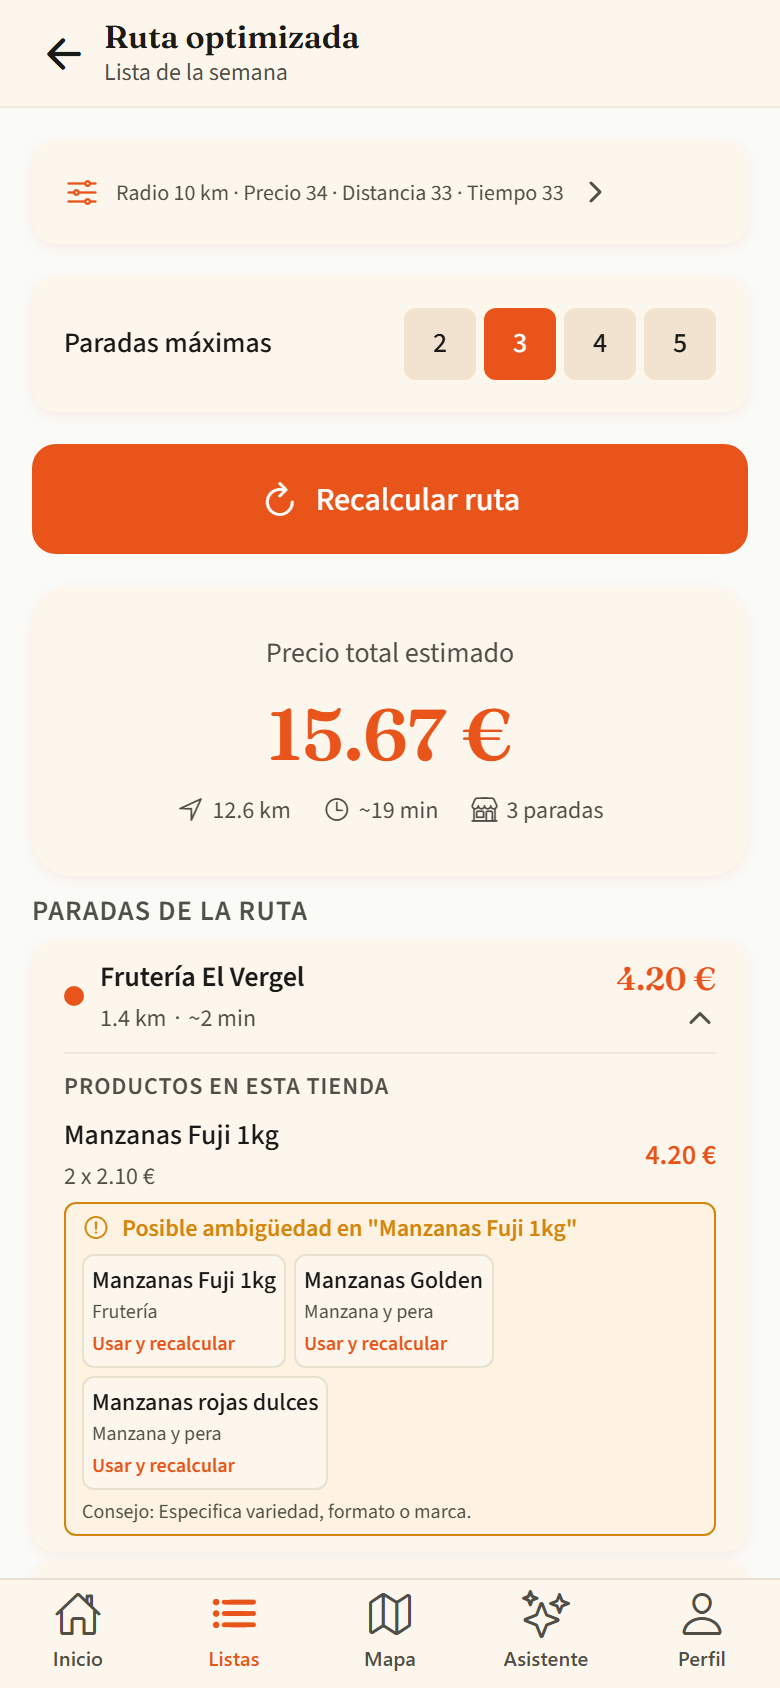
\includegraphics[width=0.40\textwidth]{diagramas/capturas/mobile-ruta.png}
\caption{Pantalla del optimizador con comparativa de rutas}
\label{fig:ui-optimizador}
\end{figure}

\section{M\'odulo OCR: captura de ticket}\label{sec:manual-ocr}

El flujo de captura de lista por c\'amara sigue un wizard de tres pasos:

\begin{enumerate}
  \item \textbf{Captura:} Acceder desde ``Mi Lista'' \textrightarrow{} icono de c\'amara.
    Apuntar la c\'amara al ticket o lista escrita. Se puede usar la galer\'ia como alternativa.
  \item \textbf{Revisi\'on:} La app muestra los productos reconocidos con nivel de confianza
    (chip de color: verde $\geq$ 80\%, amarillo 50--79\%, rojo $<$ 50\%).
    El usuario puede corregir el texto de cualquier \'item inline o eliminar los no deseados.
  \item \textbf{Confirmaci\'on:} Seleccionar la lista destino (existente o nueva) y confirmar
    para a\~nadir todos los \'items reconocidos.
\end{enumerate}

\begin{figure}[htbp]
\centering
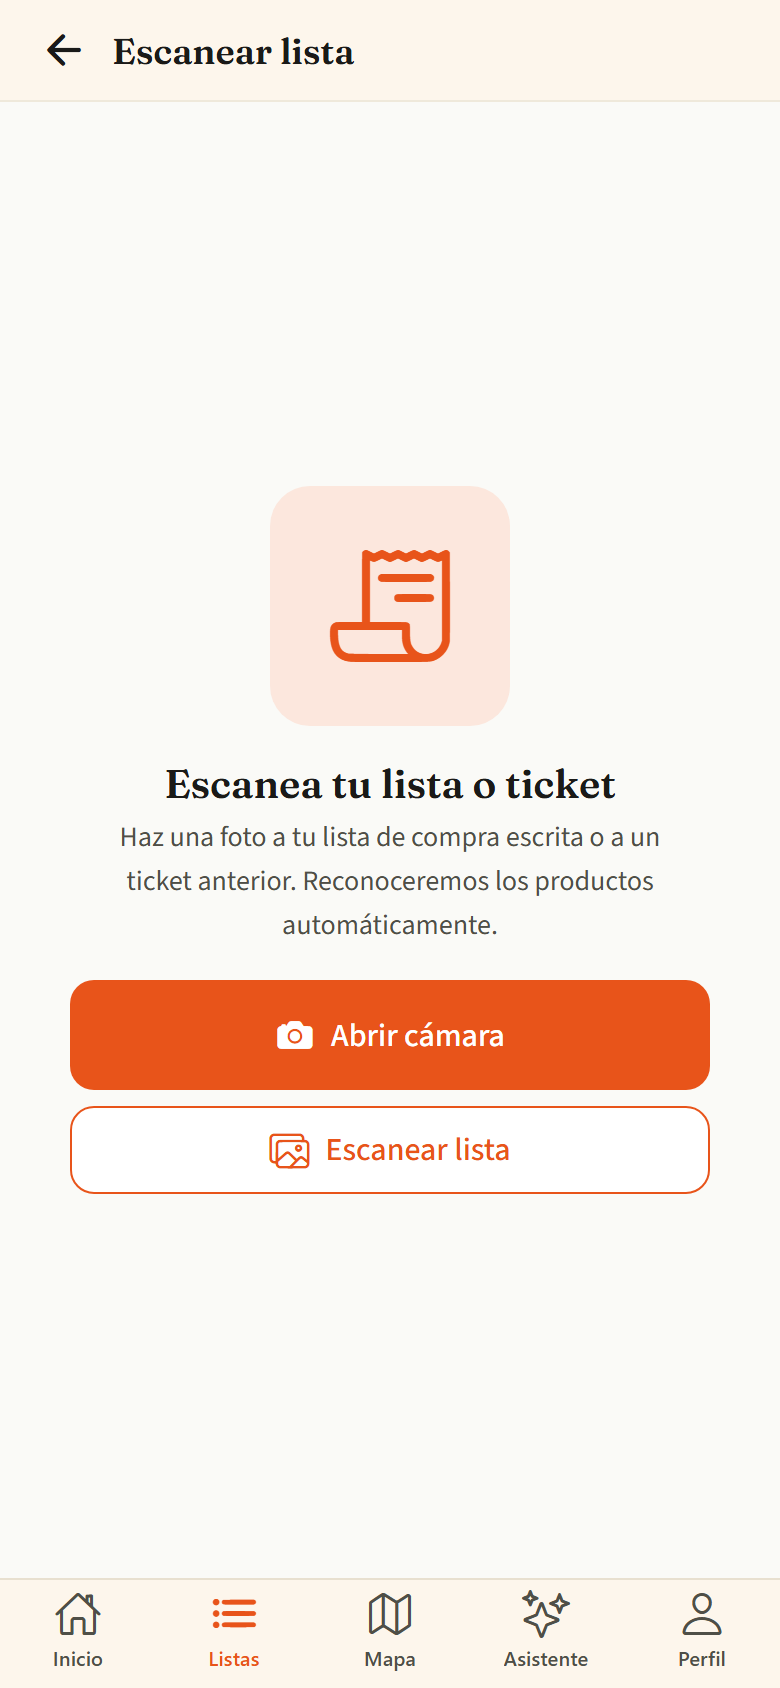
\includegraphics[width=0.32\textwidth]{diagramas/capturas/mobile-ocr-captura.png}
\hfill
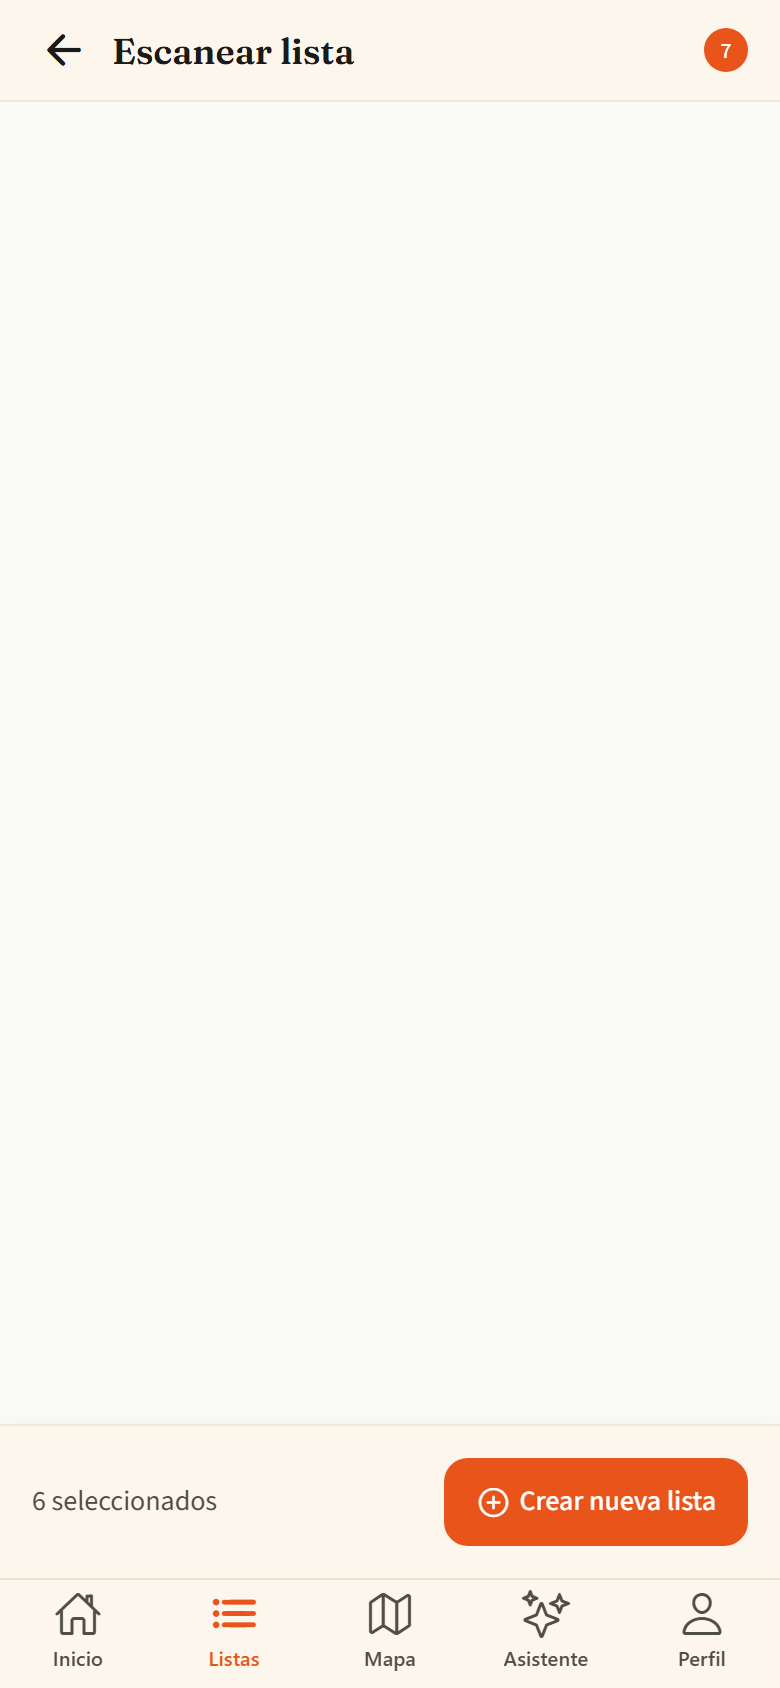
\includegraphics[width=0.32\textwidth]{diagramas/capturas/mobile-ocr-revision.png}
\caption{Flujo OCR: captura de ticket (izquierda) y revisi\'on de \'items (derecha)}
\label{fig:ui-ocr}
\end{figure}

\section{Asistente LLM}\label{sec:manual-asistente}

La pantalla del asistente sigue el patr\'on de chat est\'andar:

\begin{itemize}
  \item Mensajes del usuario alineados a la derecha (burbuja verde).
  \item Respuestas del asistente alineadas a la izquierda (burbuja gris).
  \item Las respuestas con productos, precios o tiendas incluyen chips interactivos para a\~nadir
    el producto a la lista activa directamente desde el chat.
  \item El asistente s\'olo responde preguntas relacionadas con la compra dom\'estica. Si se hace
    una pregunta fuera de ese \'ambito, responde educadamente indicando su alcance.
\end{itemize}

\begin{figure}[htbp]
\centering
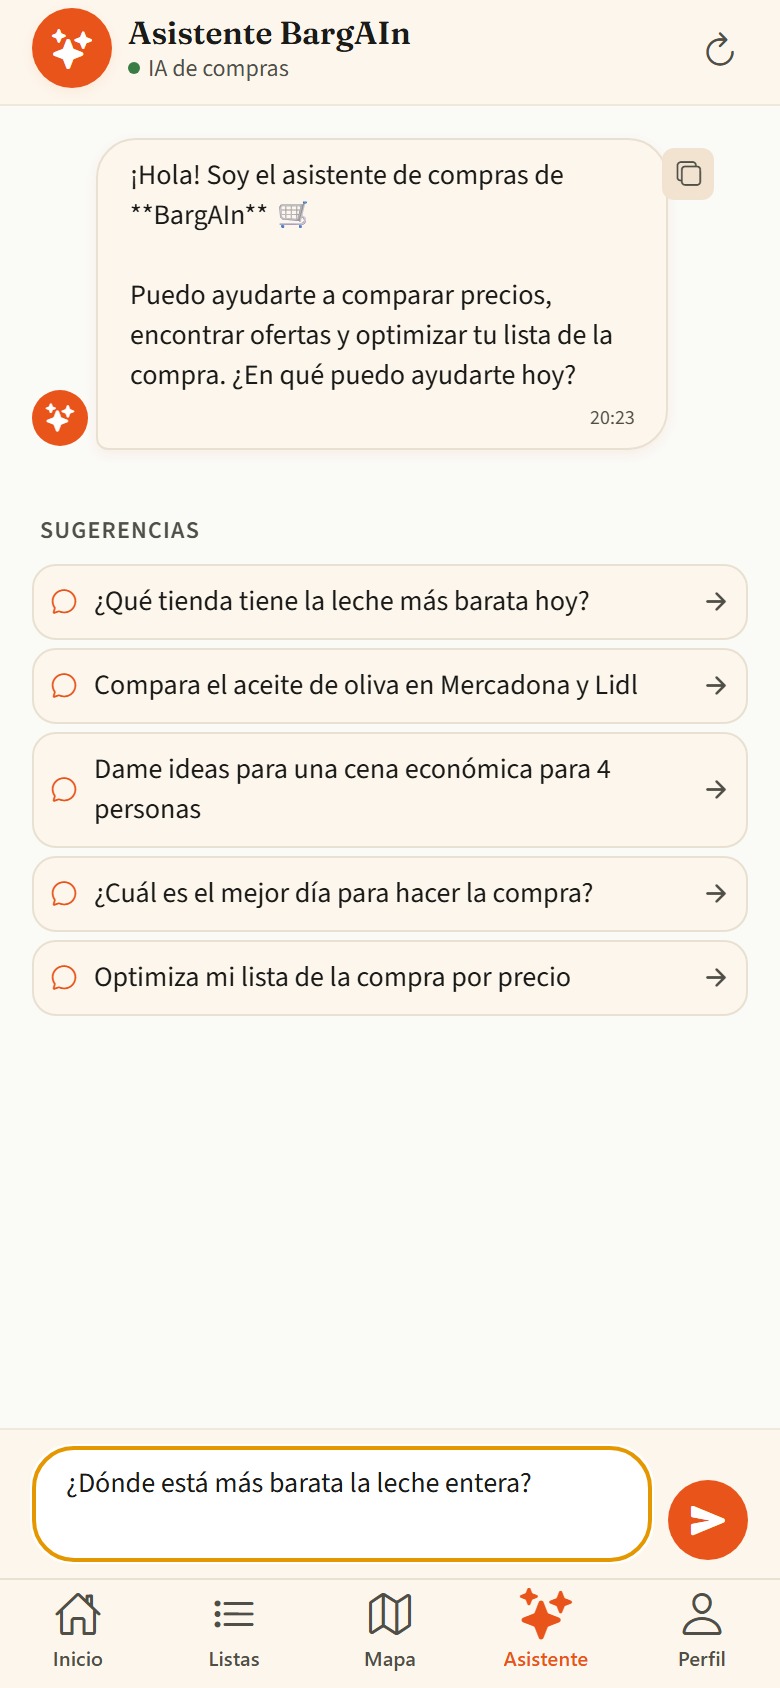
\includegraphics[width=0.40\textwidth]{diagramas/capturas/mobile-asistente.png}
\caption{Pantalla del asistente conversacional LLM}
\label{fig:ui-asistente}
\end{figure}

\section{Checklist en bloqueo de iPhone}\label{sec:manual-lockscreen}

Desde la pantalla de ruta optimizada, el bot\'on ``Checklist en bloqueo'' publica una notificaci\'on
interactiva con las acciones de marcar cada producto como comprado. Al pulsar una acci\'on en
pantalla bloqueada, el \'item se marca como comprado y la notificaci\'on se actualiza.

\section{Portal Business (web)}\label{sec:manual-business}

Para cuentas PYME, el portal web (\texttt{/business}) ofrece:

\begin{enumerate}
  \item \textbf{Registro:} Formulario de onboarding con datos del negocio (nombre, CIF, direcci\'on,
    web). La cuenta queda en estado ``pendiente'' hasta que un administrador la aprueba.
  \item \textbf{Gesti\'on de precios:} Tabla editable con todos los productos del negocio y sus
    precios actuales. Actualizaci\'on individual o mediante carga masiva en CSV.
  \item \textbf{Gesti\'on de promociones:} Crear, activar y desactivar promociones con descuento
    fijo o porcentual, fecha de fin y cantidad m\'inima.
  \item \textbf{Perfil de negocio:} Editar descripci\'on, horario, tel\'efono, imagen.
  \item \textbf{Estad\'isticas:} N\'umero de visualizaciones del perfil y comparativa de precios
    con competidores del entorno (alerta autom\'atica cuando la diferencia supera el umbral
    configurado).
\end{enumerate}

\section{Uso desde el navegador web}\label{sec:manual-web}

Adem\'as del portal PYME, la aplicaci\'on de usuario final puede ejecutarse en un navegador de
escritorio reutilizando la misma app Expo. La interfaz se adapta autom\'aticamente al ancho de la
ventana y habilita conveniencias propias del escritorio (Fase 13):

\begin{itemize}
  \item \textbf{Dise\~no adaptable:} el contenido se centra a un ancho legible y los cat\'alogos y
    listados muestran varias columnas (2--4) en pantallas anchas. En el mapa, el panel de tiendas
    se ancla a la derecha en lugar de mostrarse debajo.
  \item \textbf{Rat\'on y teclado:} atajo \texttt{Cmd/Ctrl+K} para enfocar el buscador,
    \texttt{Enter} para a\~nadir un producto a la lista y \texttt{Esc} para cerrar di\'alogos, con
    realces \emph{hover} sobre tarjetas y botones. El campo del asistente recibe el foco
    autom\'aticamente al abrir la pantalla.
  \item \textbf{Reordenar listas:} en el detalle de una lista se pueden arrastrar los \'items para
    reordenarlos (\emph{drag-and-drop}); el nuevo orden es v\'alido durante la sesi\'on.
  \item \textbf{Exportar y compartir:} botones para exportar la lista (\texttt{.txt}), la
    comparativa de precios (\texttt{.csv}) y la ruta, copiar la direcci\'on de una tienda al
    portapapeles y compartir el enlace directo a una lista o tienda.
  \item \textbf{Enlaces directos:} cada pantalla relevante tiene una URL propia, por lo que se
    puede compartir o guardar como marcador el estado actual (por ejemplo, una b\'usqueda concreta
    del cat\'alogo mediante \texttt{?q=}).
\end{itemize}

\section{Galer\'ia de capturas de la aplicaci\'on}\label{sec:manual-galeria}

Esta secci\'on recoge capturas reales de cada pantalla y funcionalidad de la aplicaci\'on
desplegada, agrupadas por contexto de uso: aplicaci\'on m\'ovil de usuario (viewport
390$\times$844), aplicaci\'on web de usuario (escritorio, 1440$\times$900) y portal web para
PYMEs. Todas las im\'agenes residen en \texttt{diagramas/capturas/}.

\subsection{Aplicaci\'on m\'ovil (usuario)}\label{subsec:galeria-movil}

\begin{figure}[htbp]
\centering
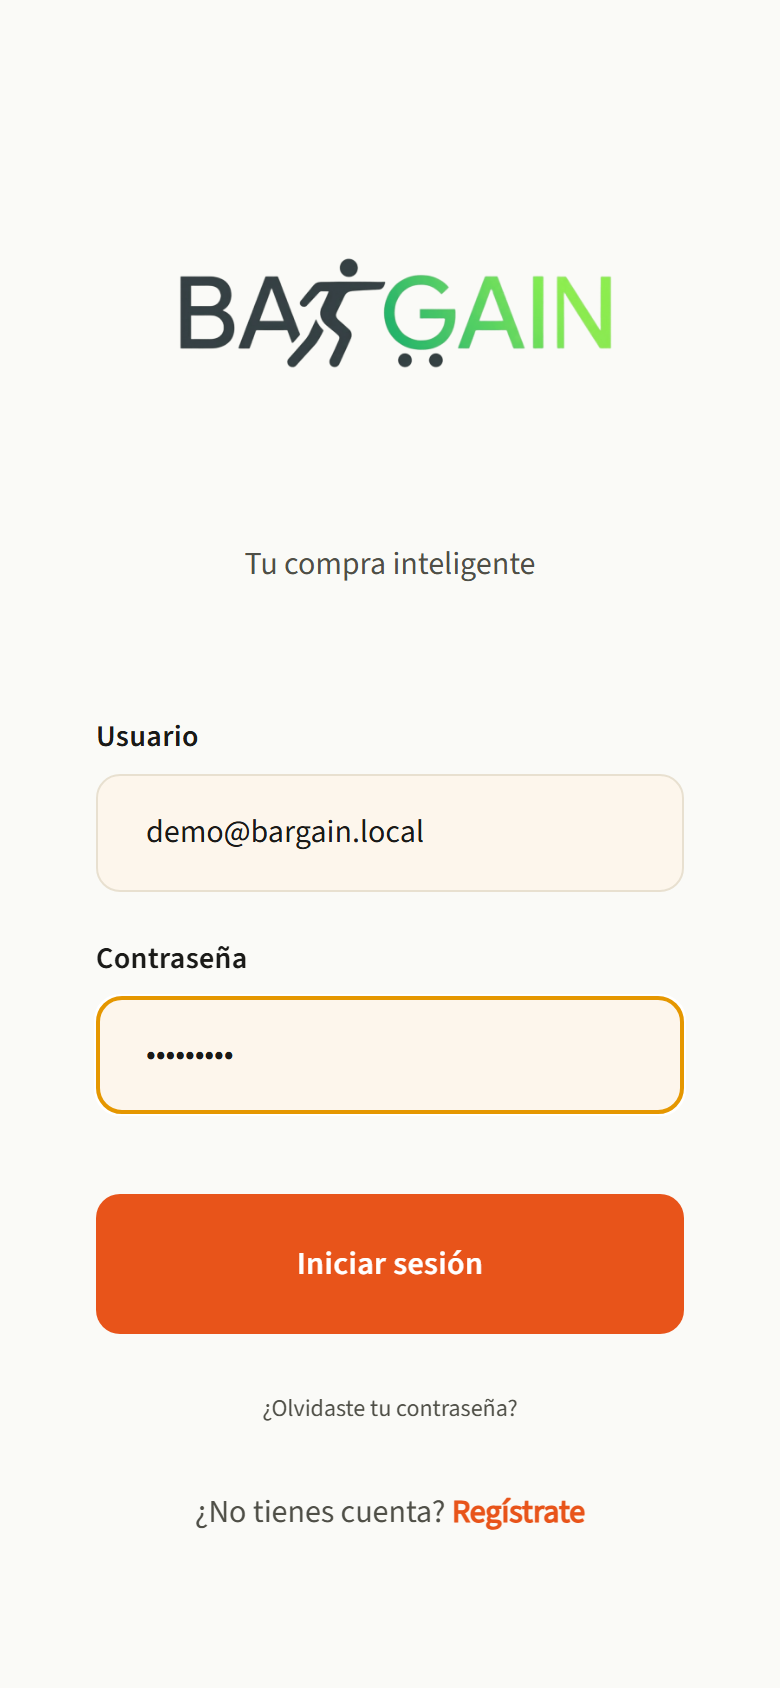
\includegraphics[width=0.30\textwidth]{diagramas/capturas/mobile-login.png}
\hfill
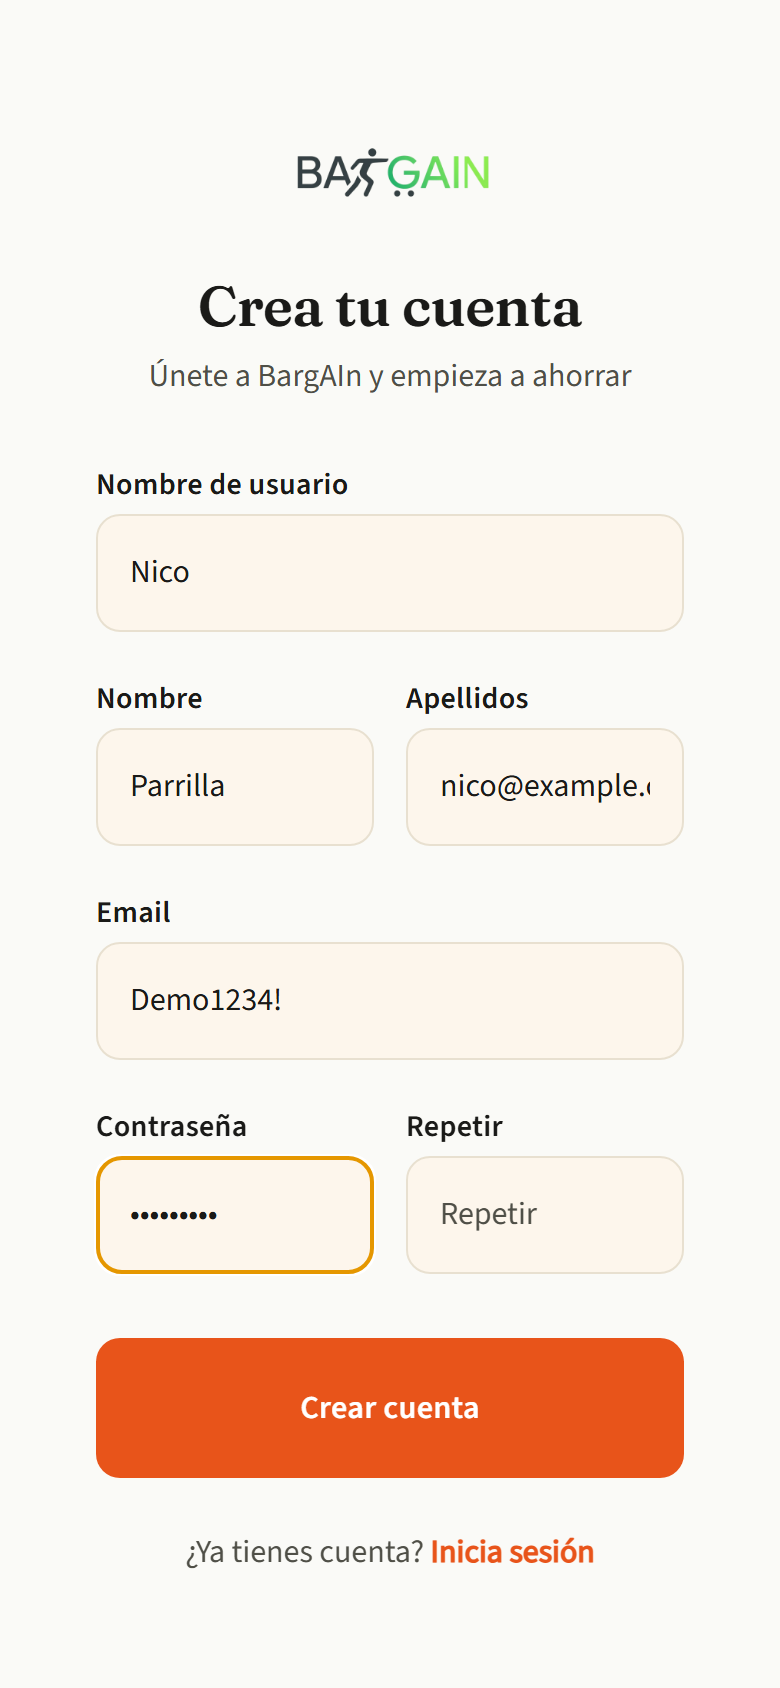
\includegraphics[width=0.30\textwidth]{diagramas/capturas/mobile-registro.png}
\caption{M\'ovil --- Inicio de sesi\'on (izquierda) y registro (derecha)}
\label{fig:cap-mobile-acceso}
\end{figure}

\begin{figure}[htbp]
\centering
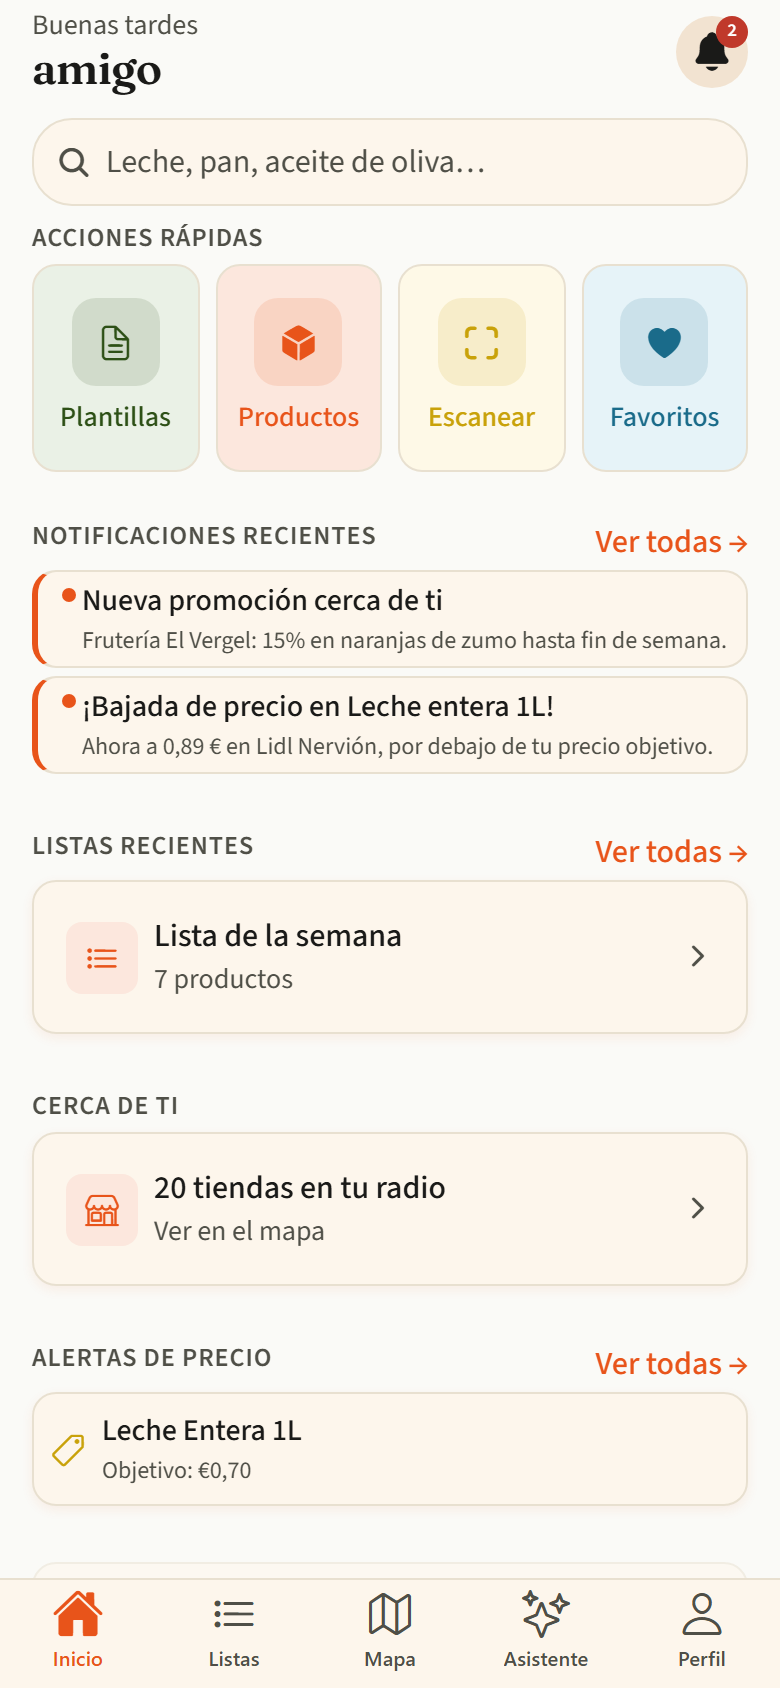
\includegraphics[width=0.30\textwidth]{diagramas/capturas/mobile-home.png}
\hfill
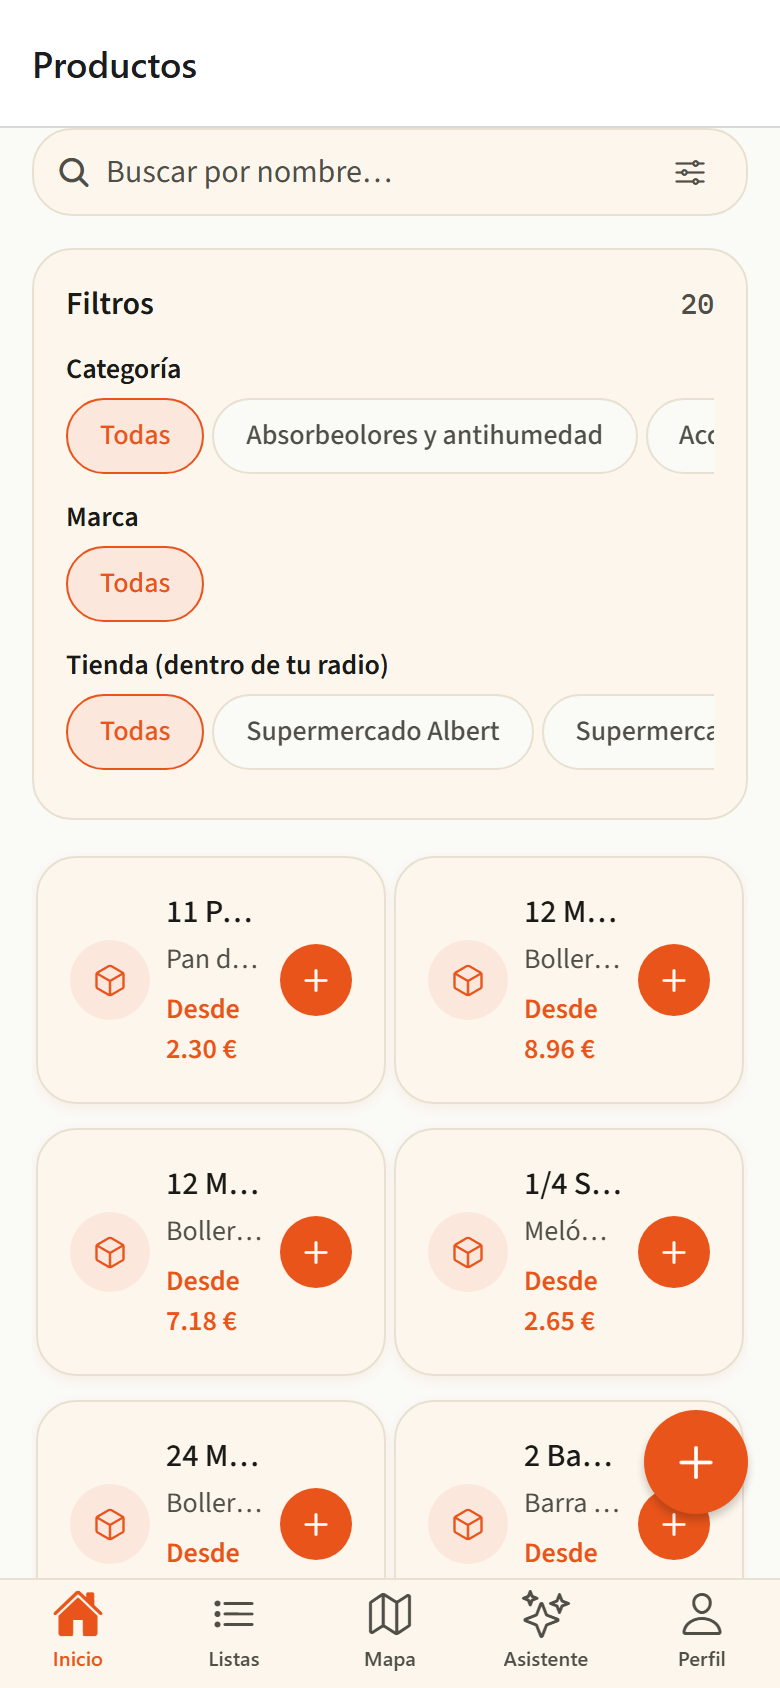
\includegraphics[width=0.30\textwidth]{diagramas/capturas/mobile-catalogo.png}
\caption{M\'ovil --- Pantalla principal (izquierda) y cat\'alogo de productos (derecha)}
\label{fig:cap-mobile-home-catalogo}
\end{figure}

\begin{figure}[htbp]
\centering
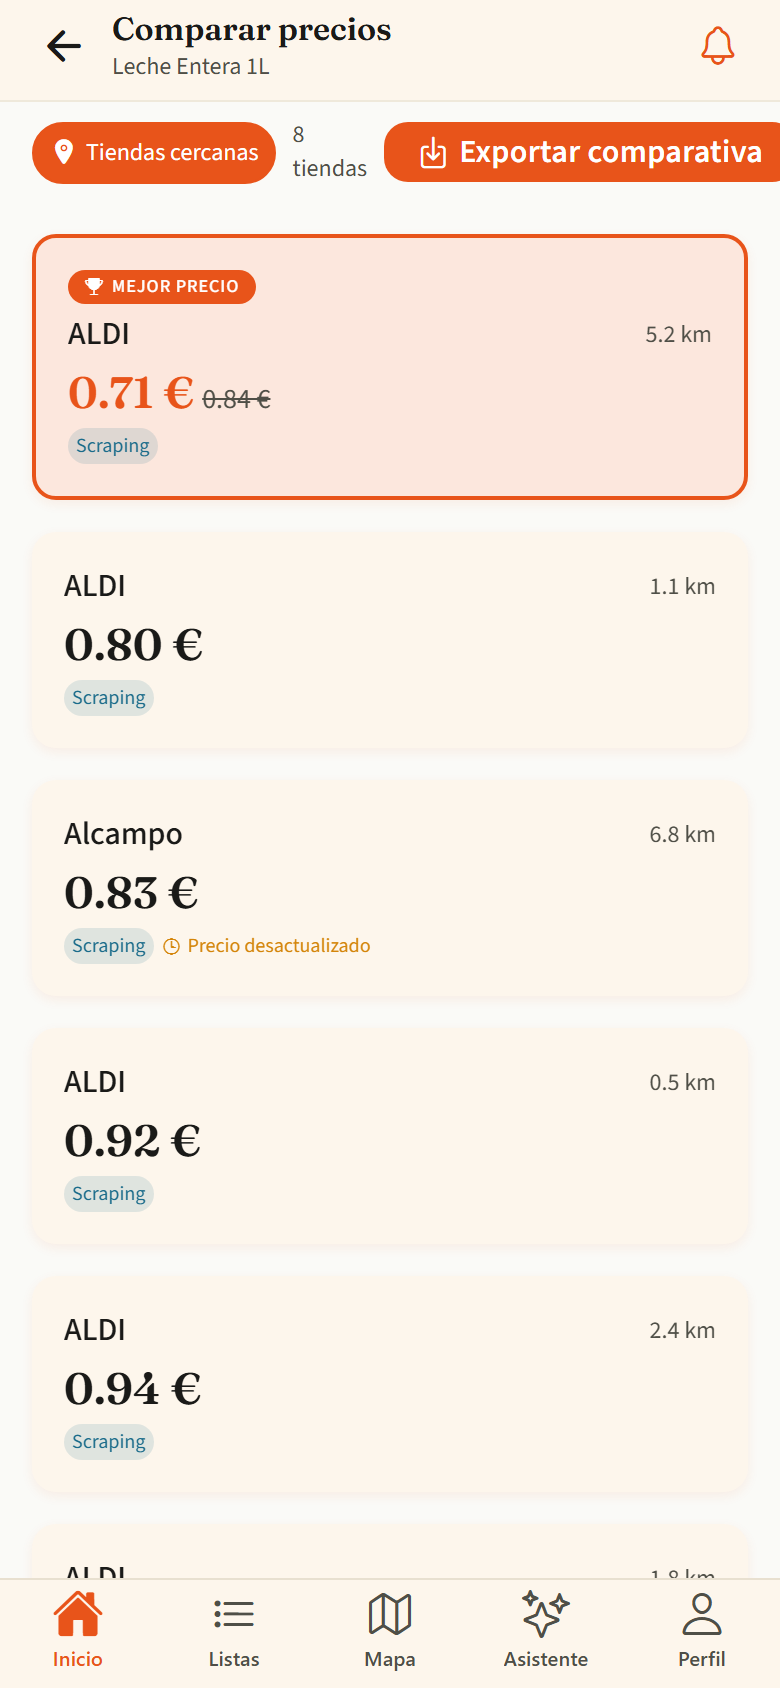
\includegraphics[width=0.30\textwidth]{diagramas/capturas/mobile-detalle-precio.png}
\hfill
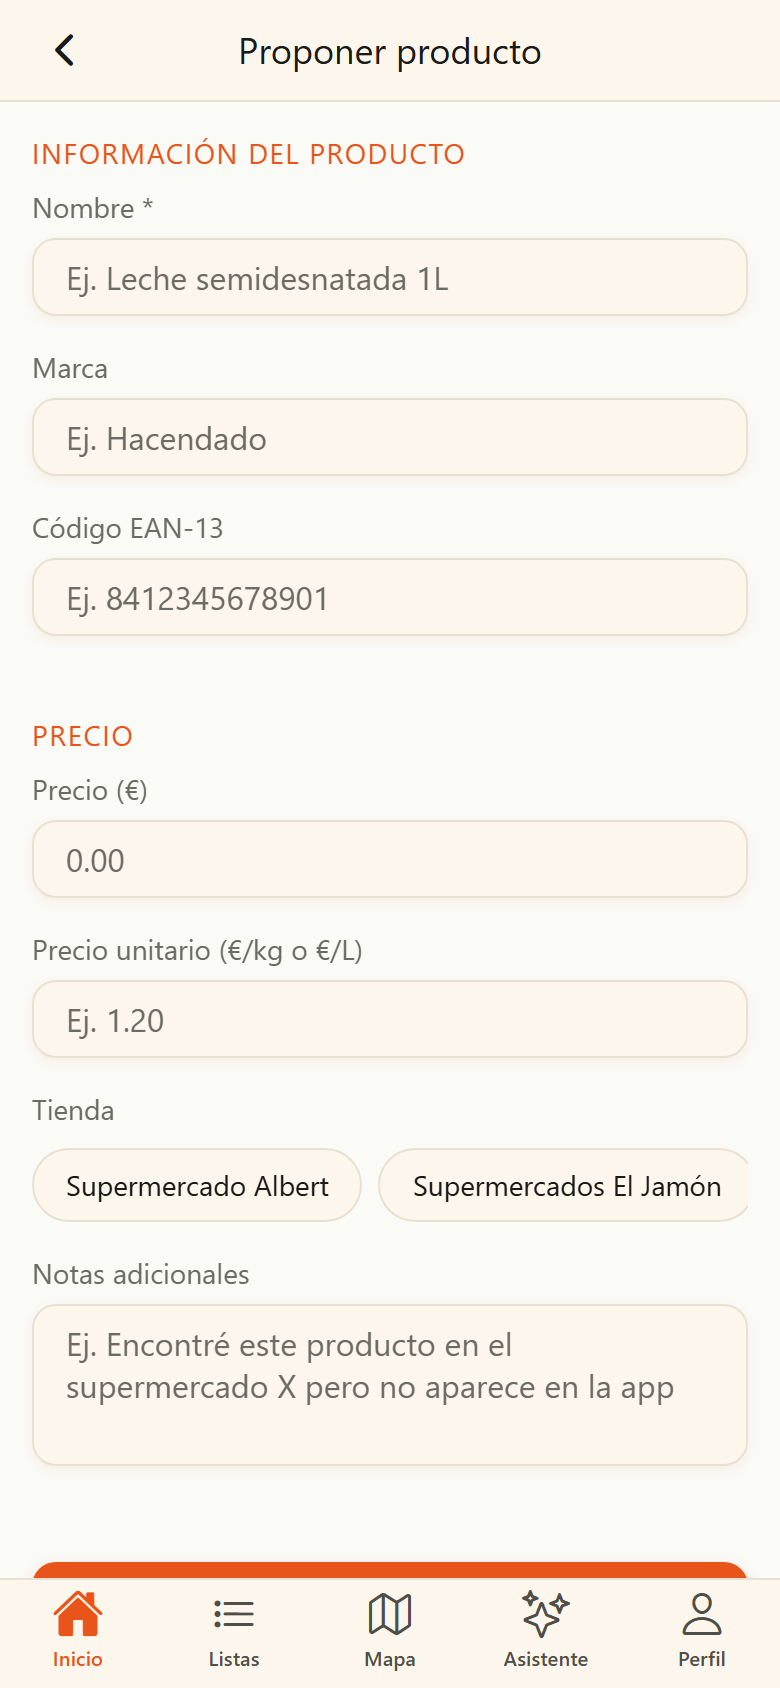
\includegraphics[width=0.30\textwidth]{diagramas/capturas/mobile-proponer.png}
\caption{M\'ovil --- Comparativa de precios por tienda (izquierda) y propuesta de producto (derecha)}
\label{fig:cap-mobile-precio-proponer}
\end{figure}

\begin{figure}[htbp]
\centering
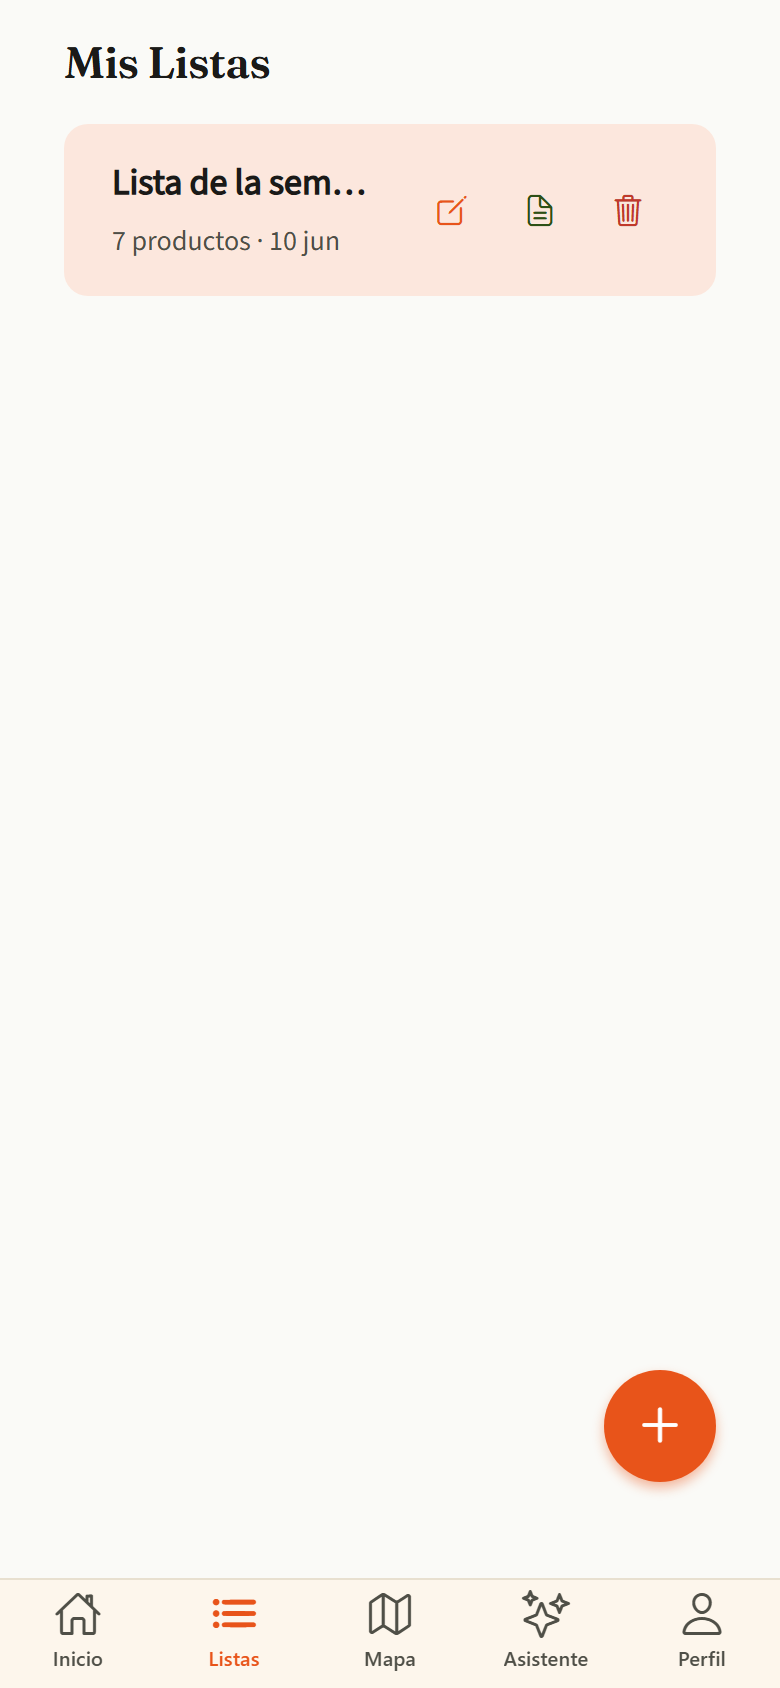
\includegraphics[width=0.30\textwidth]{diagramas/capturas/mobile-listas.png}
\hfill
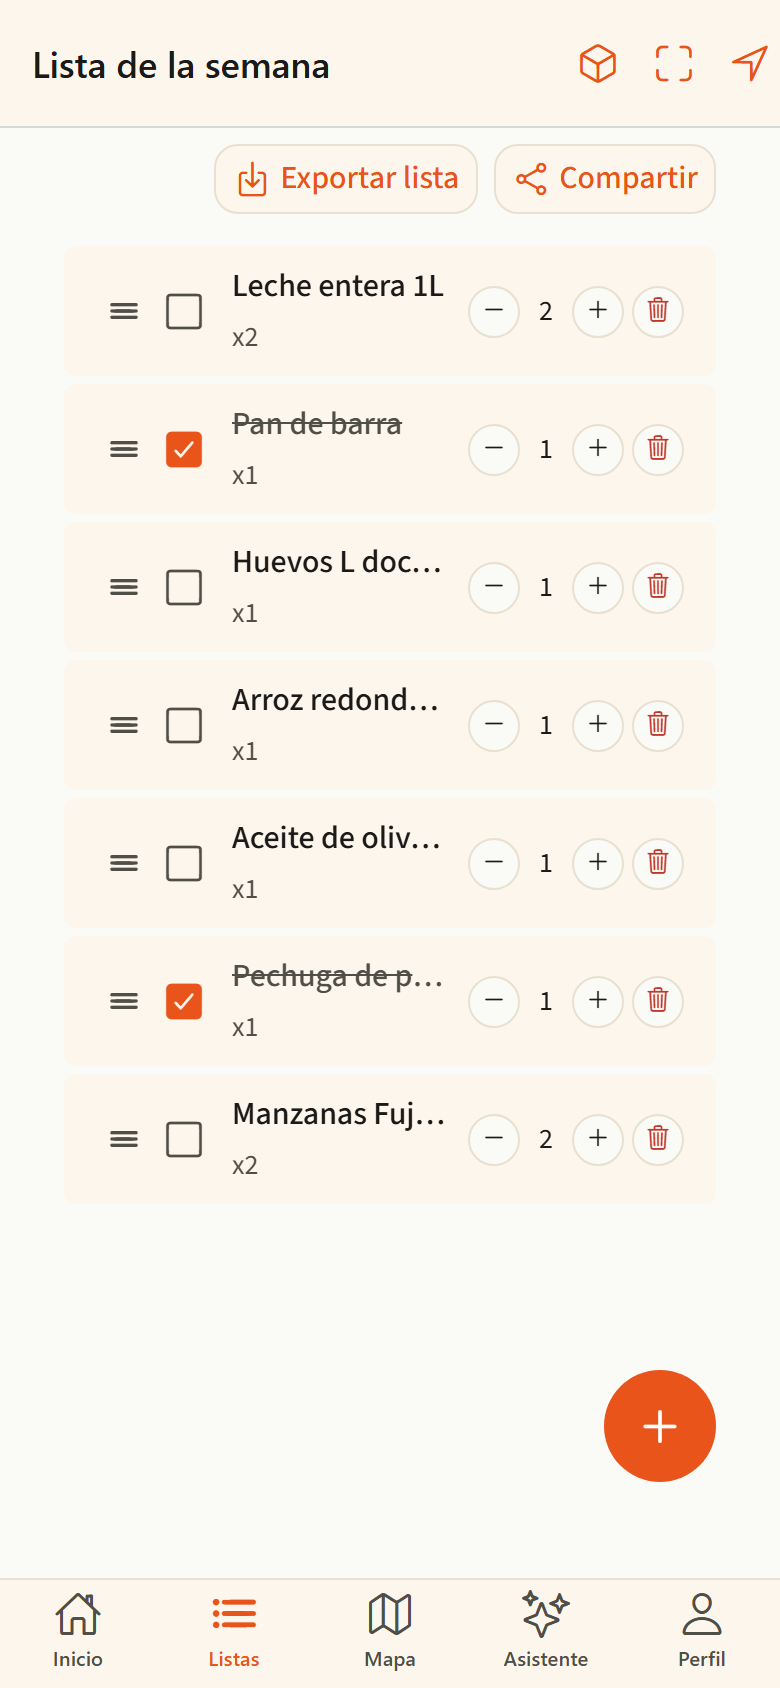
\includegraphics[width=0.30\textwidth]{diagramas/capturas/mobile-lista-detalle.png}
\caption{M\'ovil --- Listas de la compra (izquierda) y detalle de una lista (derecha)}
\label{fig:cap-mobile-listas}
\end{figure}

\clearpage

\begin{figure}[htbp]
\centering
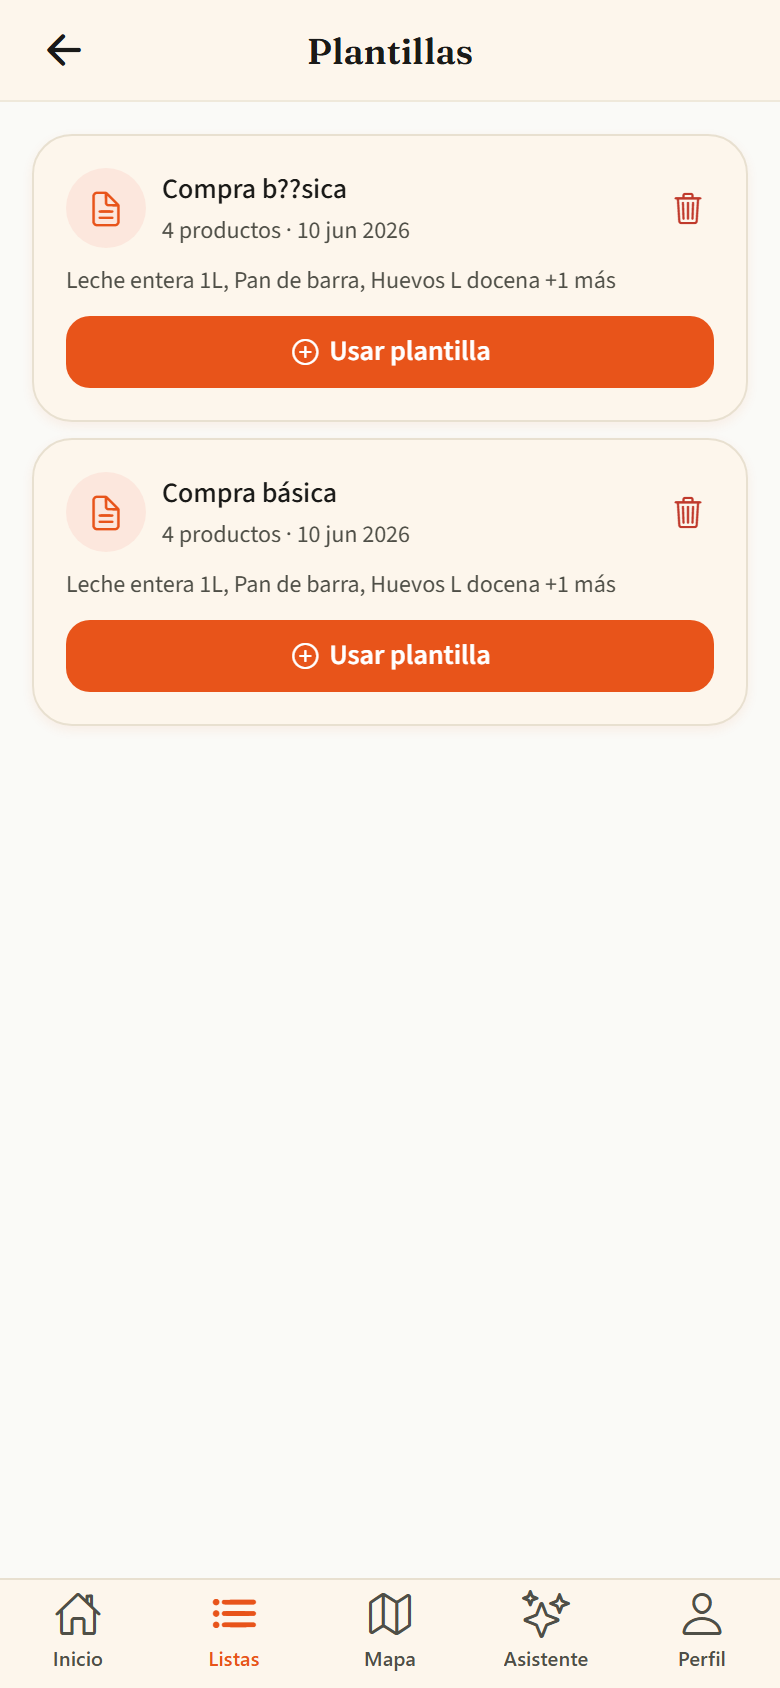
\includegraphics[width=0.30\textwidth]{diagramas/capturas/mobile-plantillas.png}
\hfill
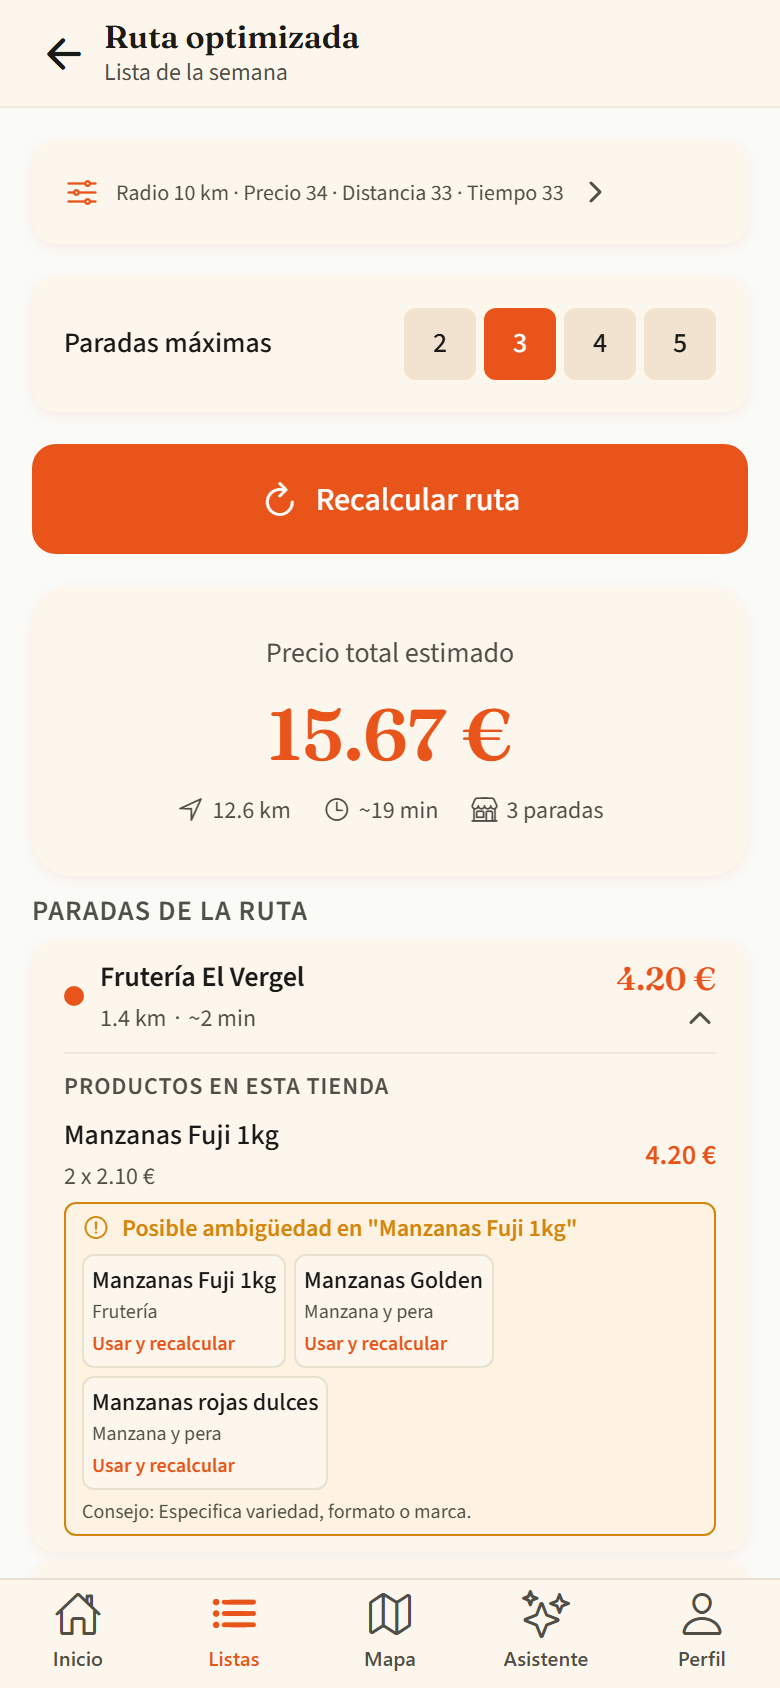
\includegraphics[width=0.30\textwidth]{diagramas/capturas/mobile-ruta.png}
\caption{M\'ovil --- Plantillas de lista (izquierda) y ruta optimizada (derecha)}
\label{fig:cap-mobile-plantillas-ruta}
\end{figure}

\begin{figure}[htbp]
\centering
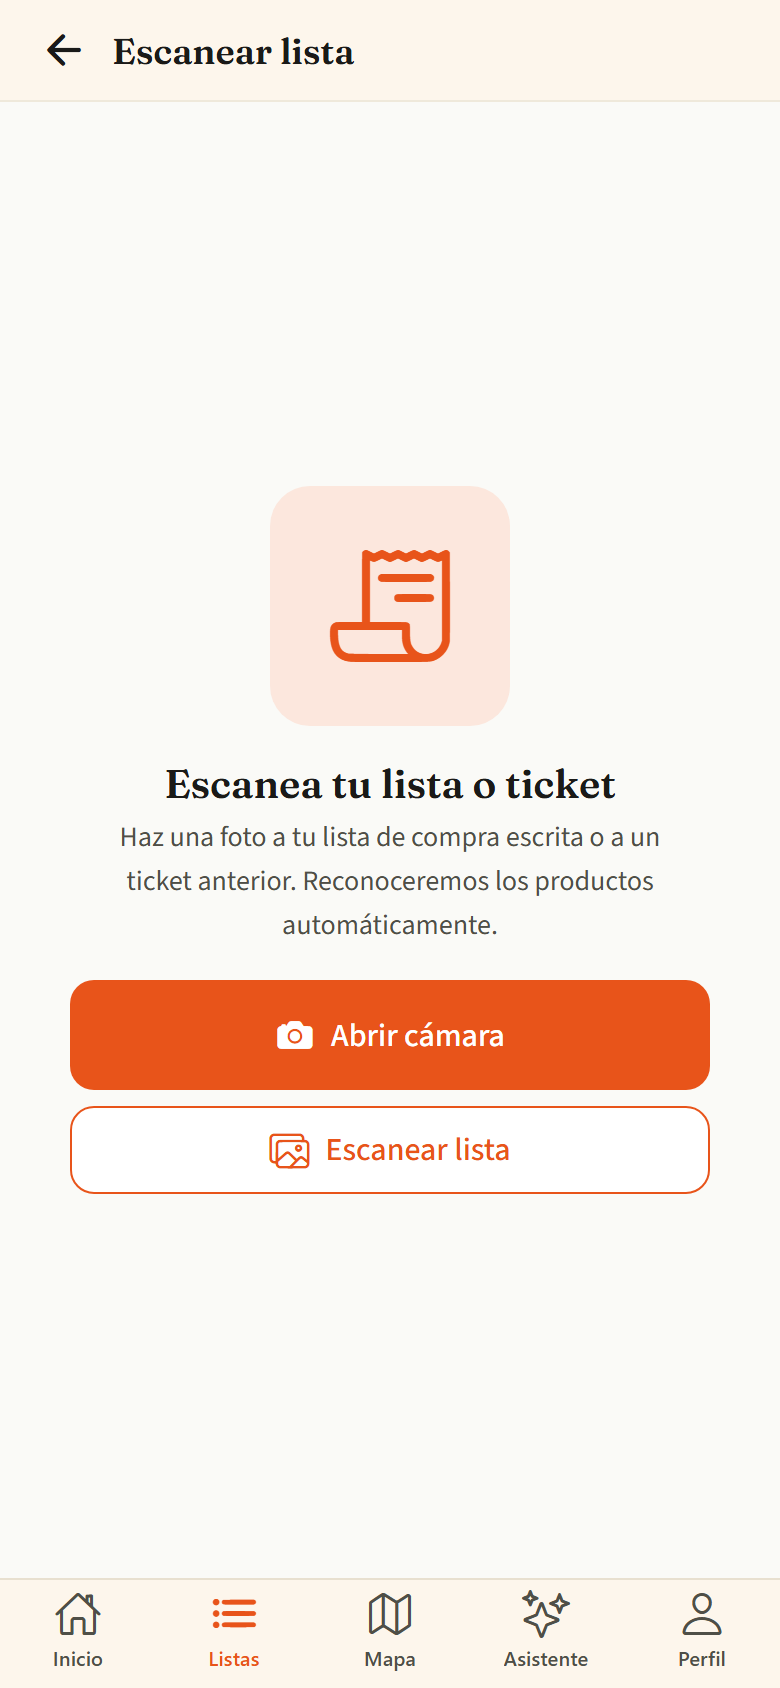
\includegraphics[width=0.30\textwidth]{diagramas/capturas/mobile-ocr-captura.png}
\hfill
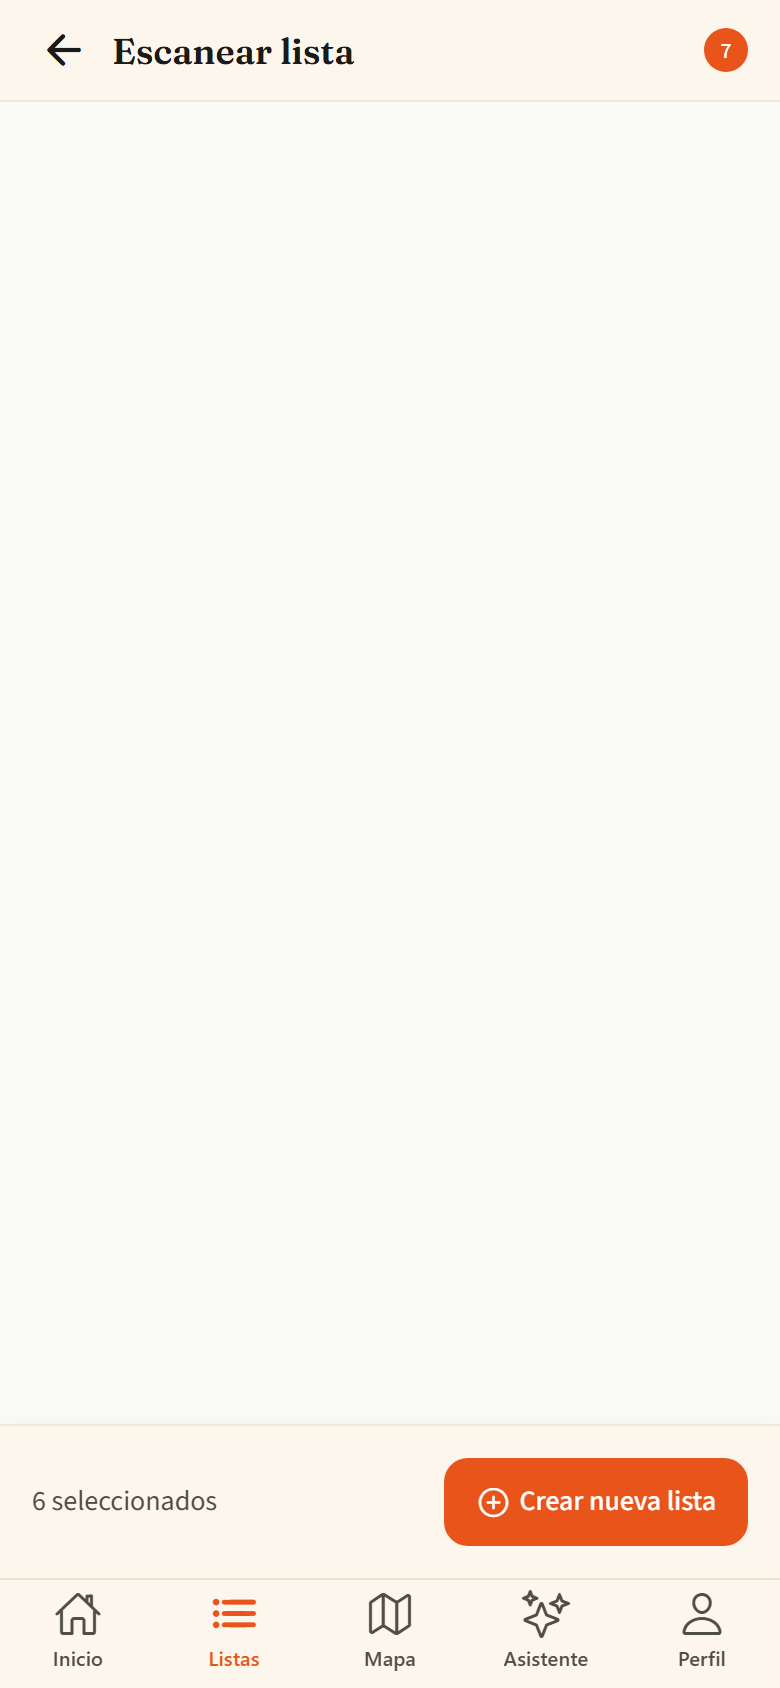
\includegraphics[width=0.30\textwidth]{diagramas/capturas/mobile-ocr-revision.png}
\caption{M\'ovil --- M\'odulo OCR: captura de ticket (izquierda) y revisi\'on de \'items (derecha)}
\label{fig:cap-mobile-ocr}
\end{figure}

\begin{figure}[htbp]
\centering
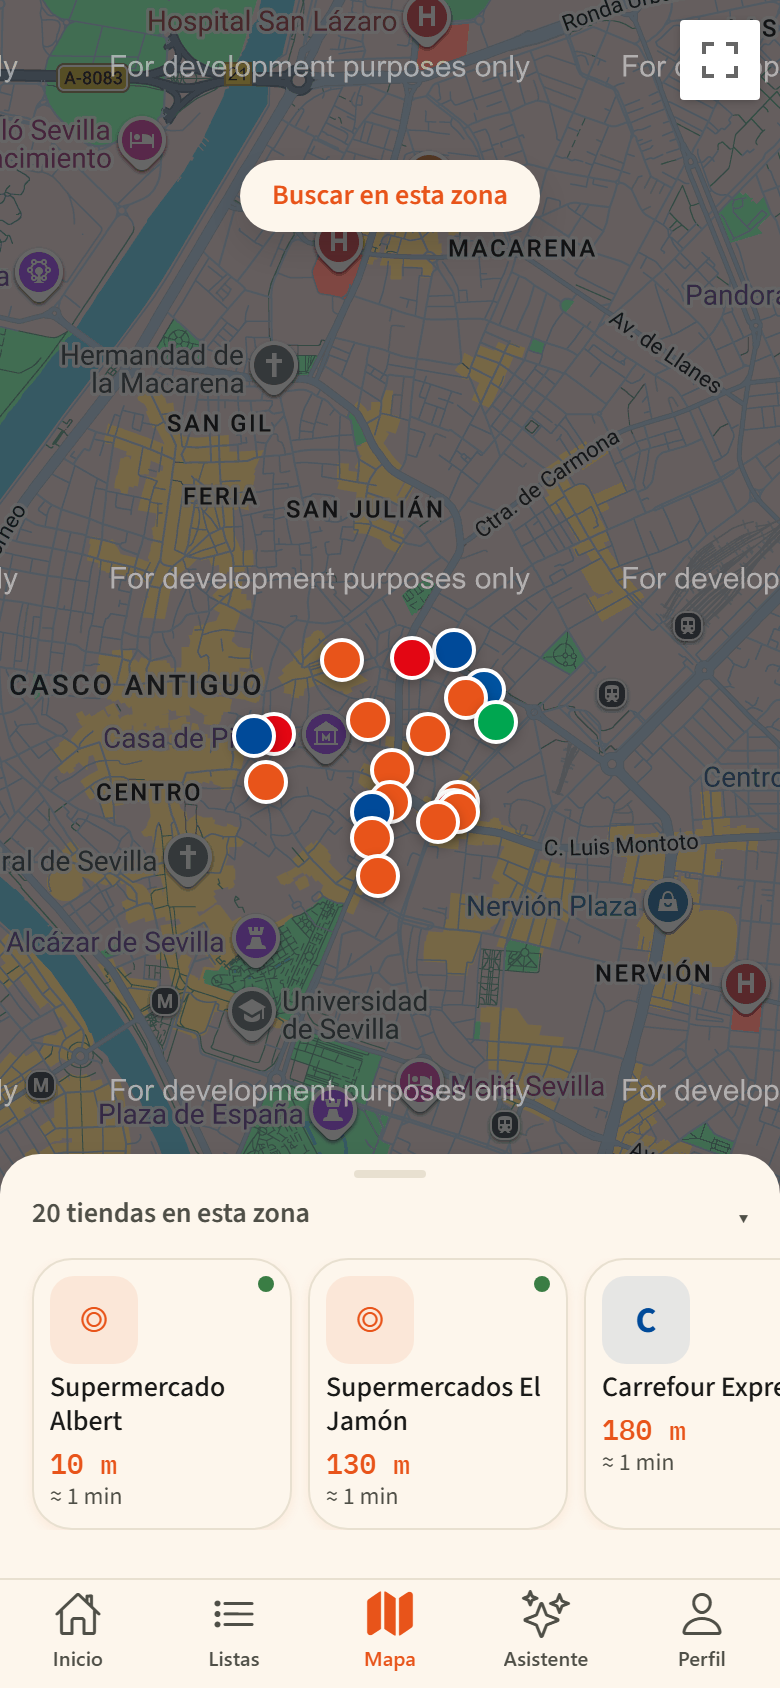
\includegraphics[width=0.30\textwidth]{diagramas/capturas/mobile-mapa.png}
\hfill
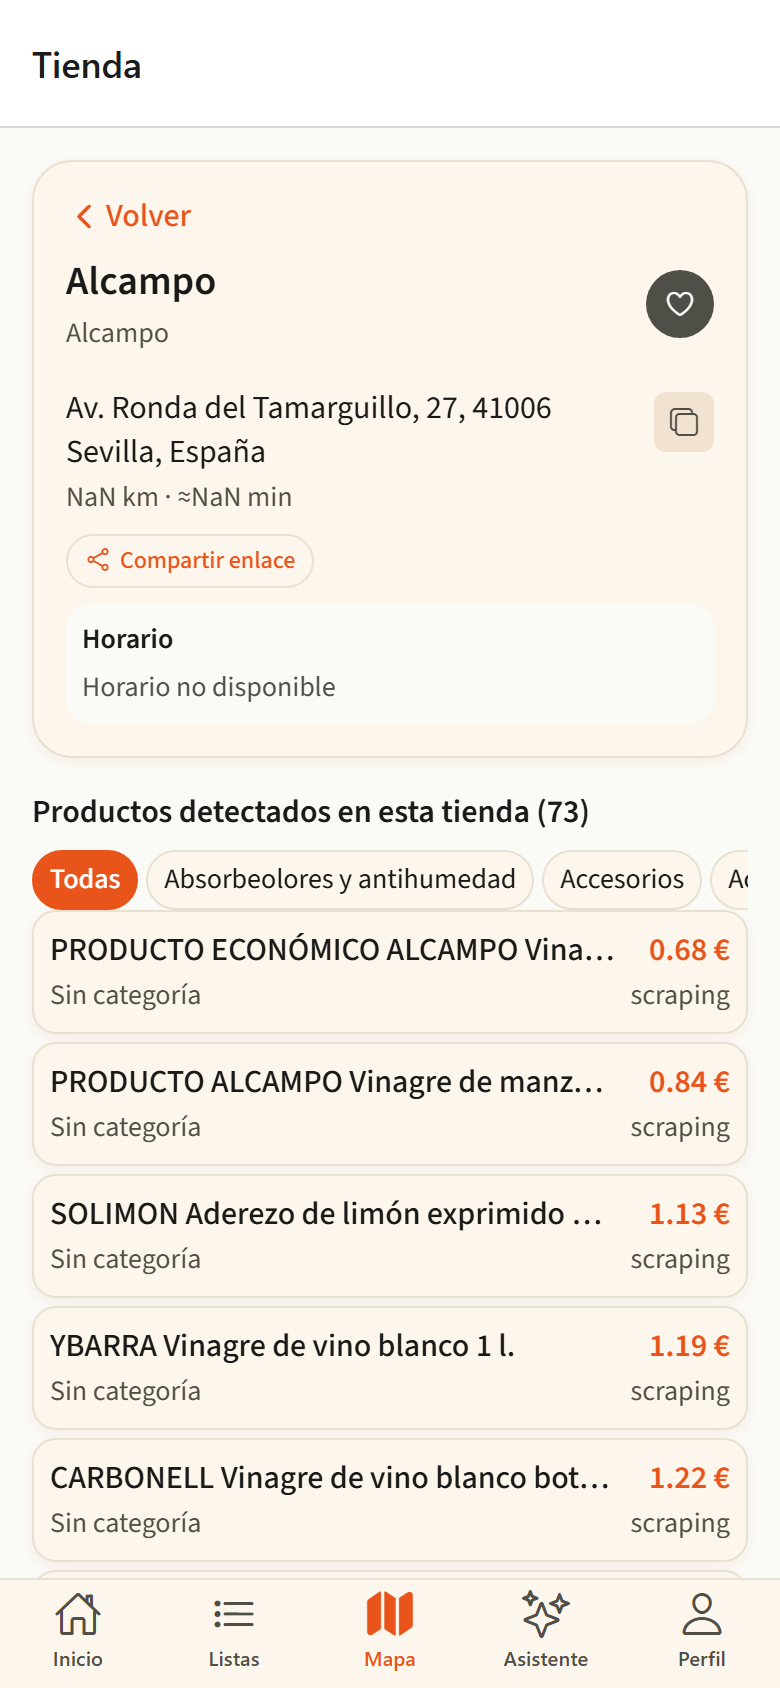
\includegraphics[width=0.30\textwidth]{diagramas/capturas/mobile-tienda-perfil.png}
\caption{M\'ovil --- Mapa de tiendas (izquierda) y perfil de tienda (derecha)}
\label{fig:cap-mobile-mapa}
\end{figure}

\begin{figure}[htbp]
\centering
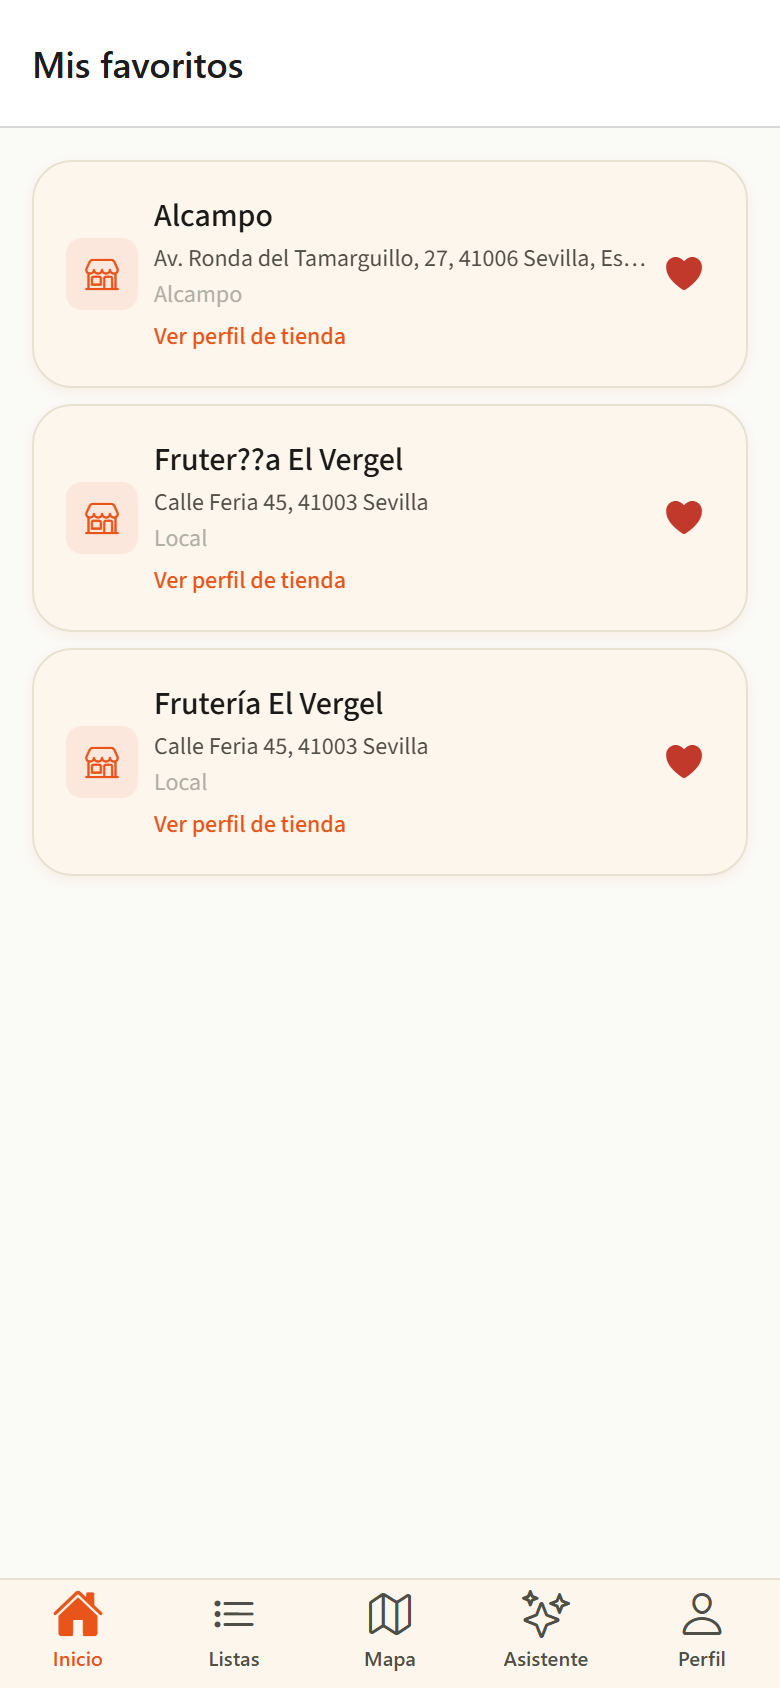
\includegraphics[width=0.30\textwidth]{diagramas/capturas/mobile-favoritas.png}
\hfill
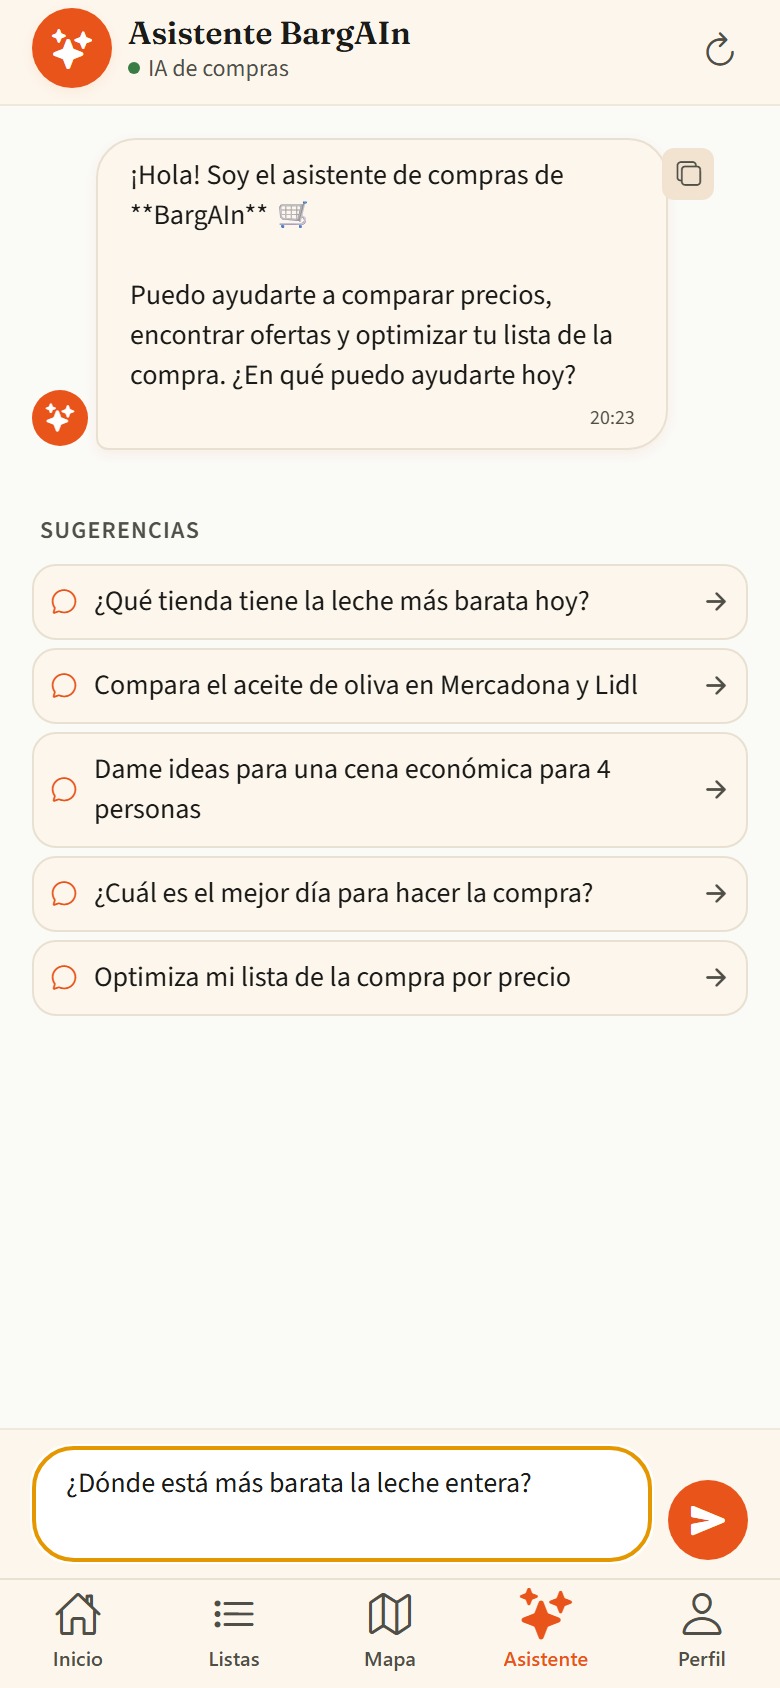
\includegraphics[width=0.30\textwidth]{diagramas/capturas/mobile-asistente.png}
\caption{M\'ovil --- Tiendas favoritas (izquierda) y asistente conversacional (derecha)}
\label{fig:cap-mobile-favoritas-asistente}
\end{figure}

\clearpage

\begin{figure}[htbp]
\centering
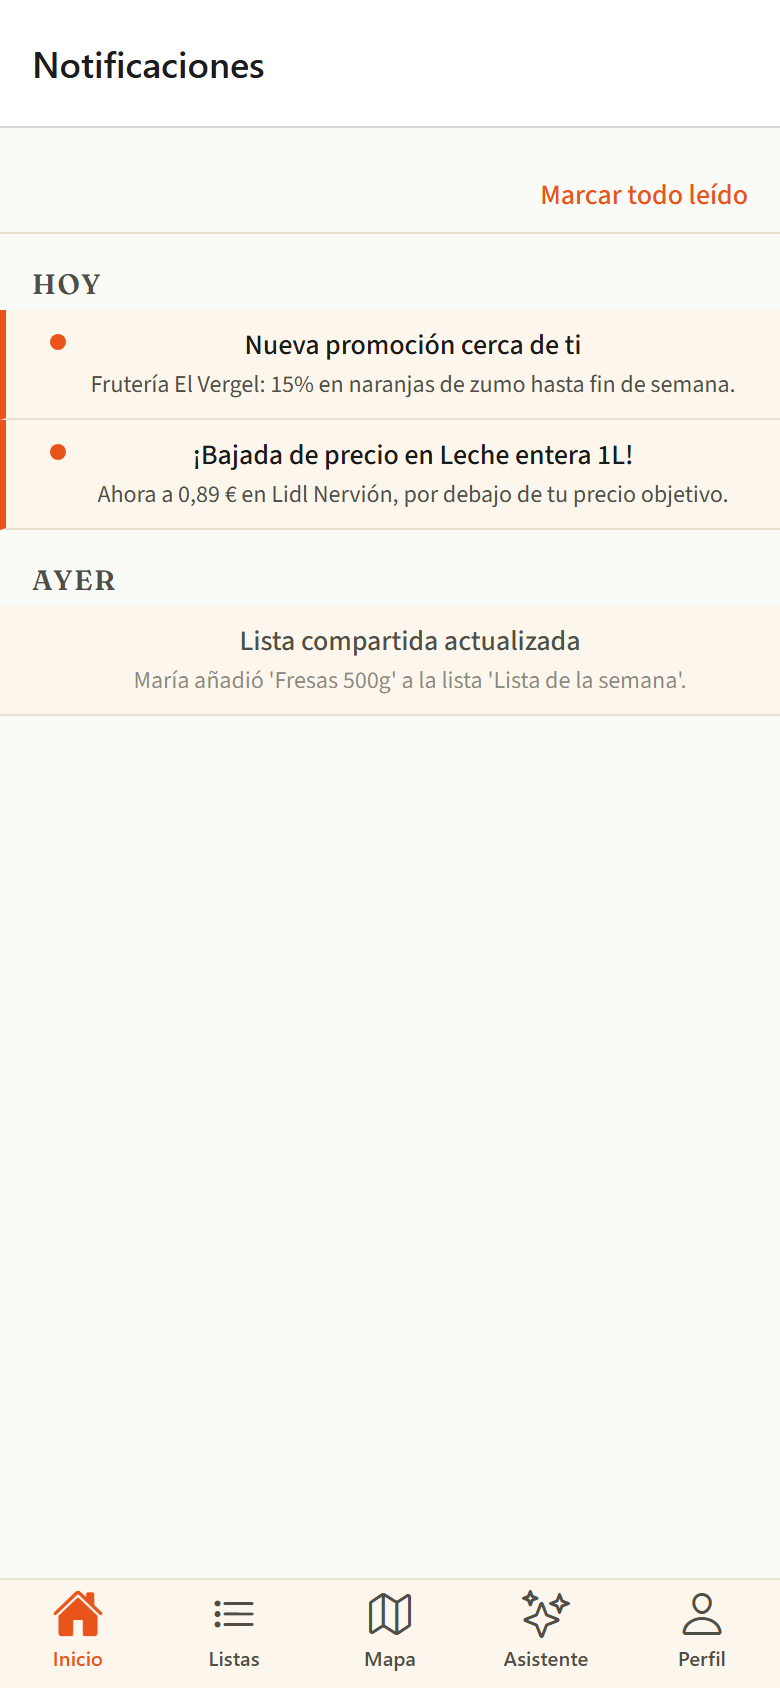
\includegraphics[width=0.30\textwidth]{diagramas/capturas/mobile-notificaciones.png}
\hfill
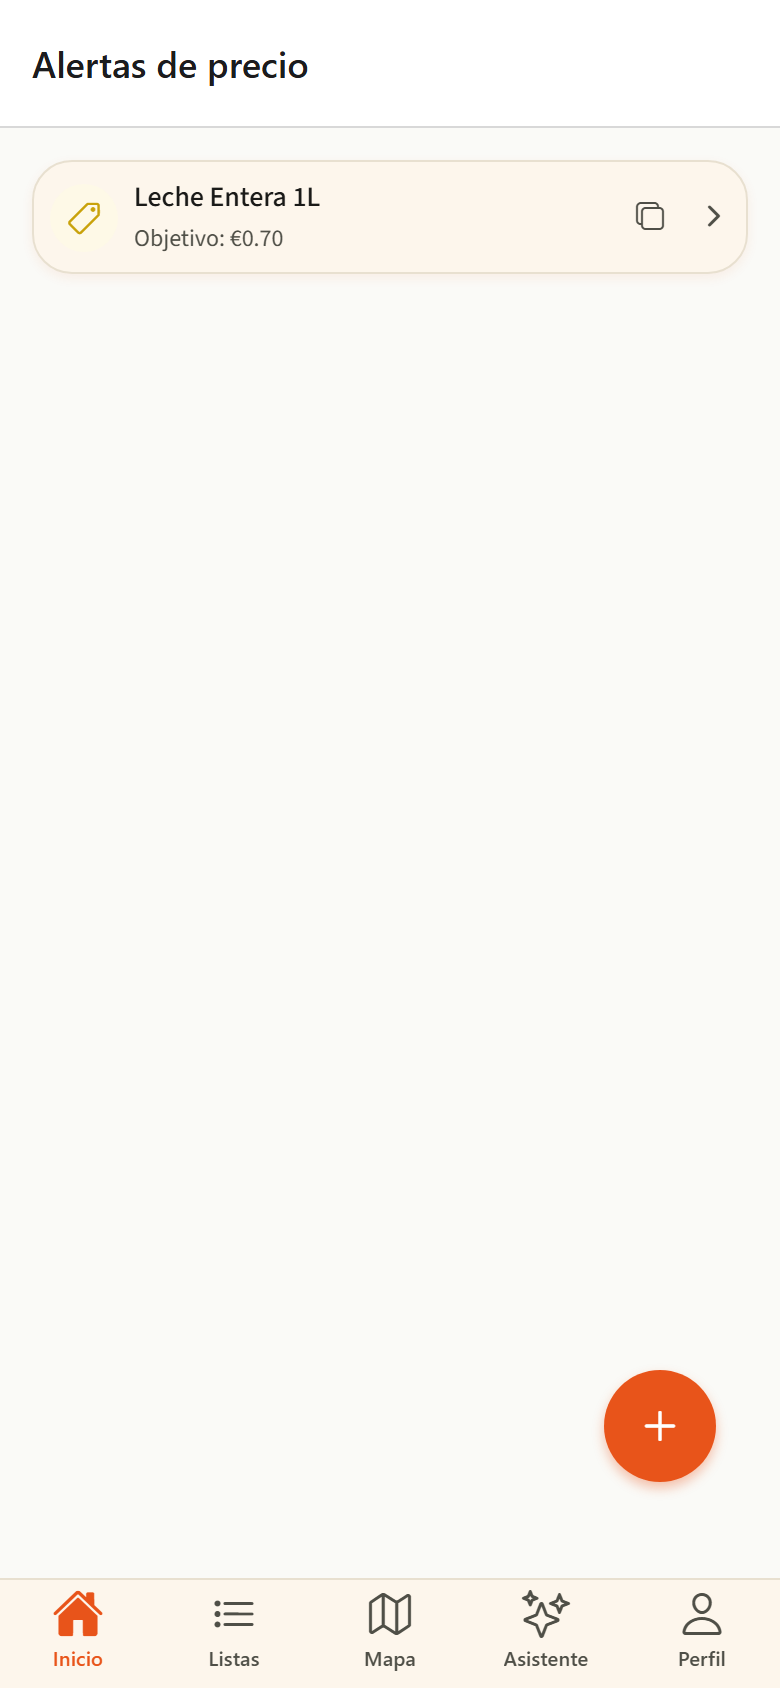
\includegraphics[width=0.30\textwidth]{diagramas/capturas/mobile-alertas.png}
\caption{M\'ovil --- Bandeja de notificaciones (izquierda) y alertas de precio (derecha)}
\label{fig:cap-mobile-notif-alertas}
\end{figure}

\begin{figure}[htbp]
\centering
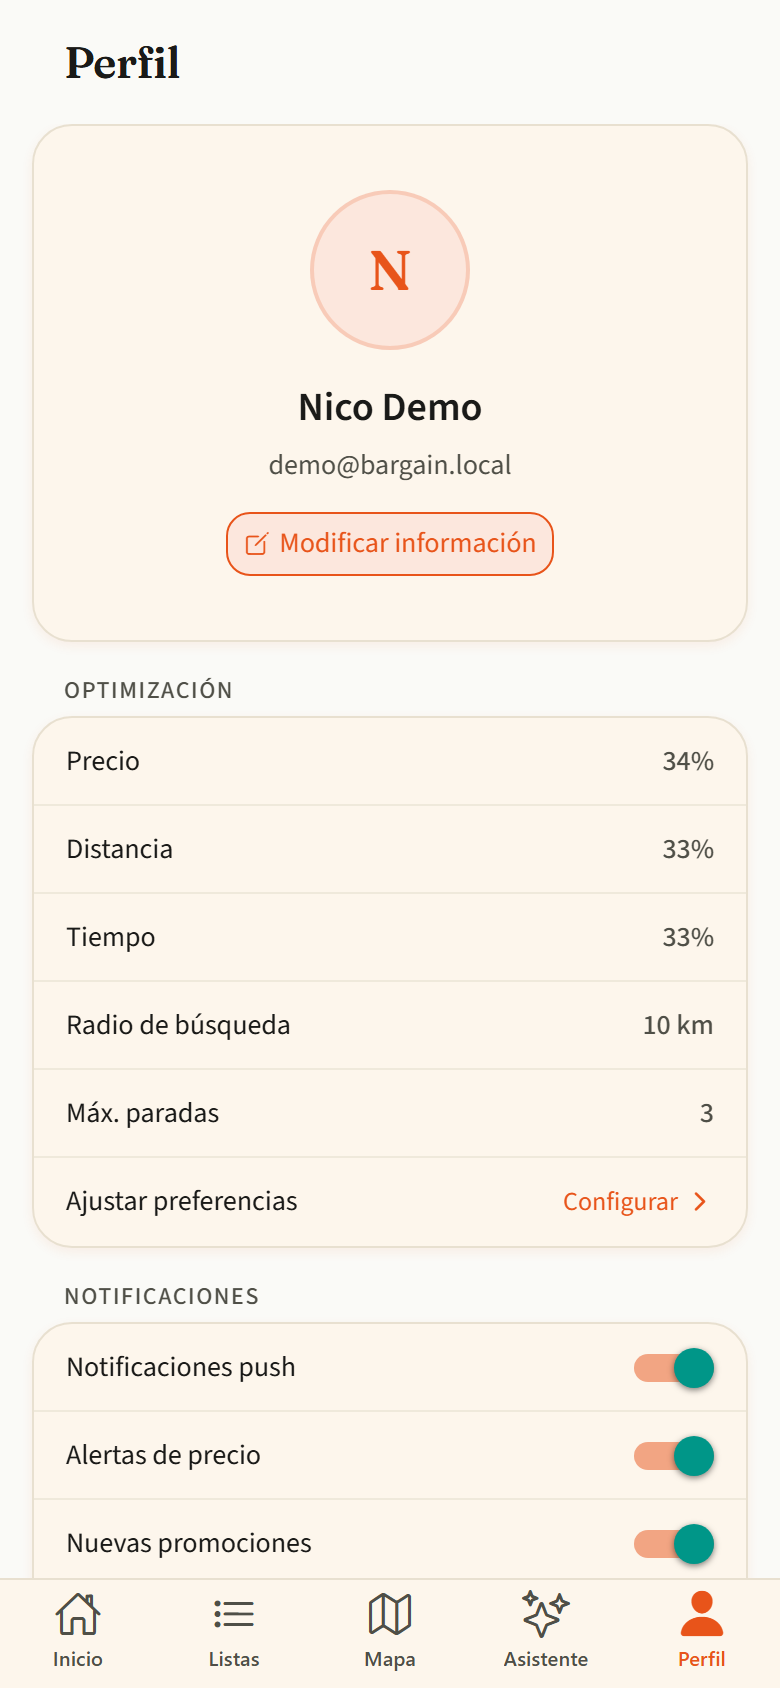
\includegraphics[width=0.30\textwidth]{diagramas/capturas/mobile-perfil.png}
\hfill
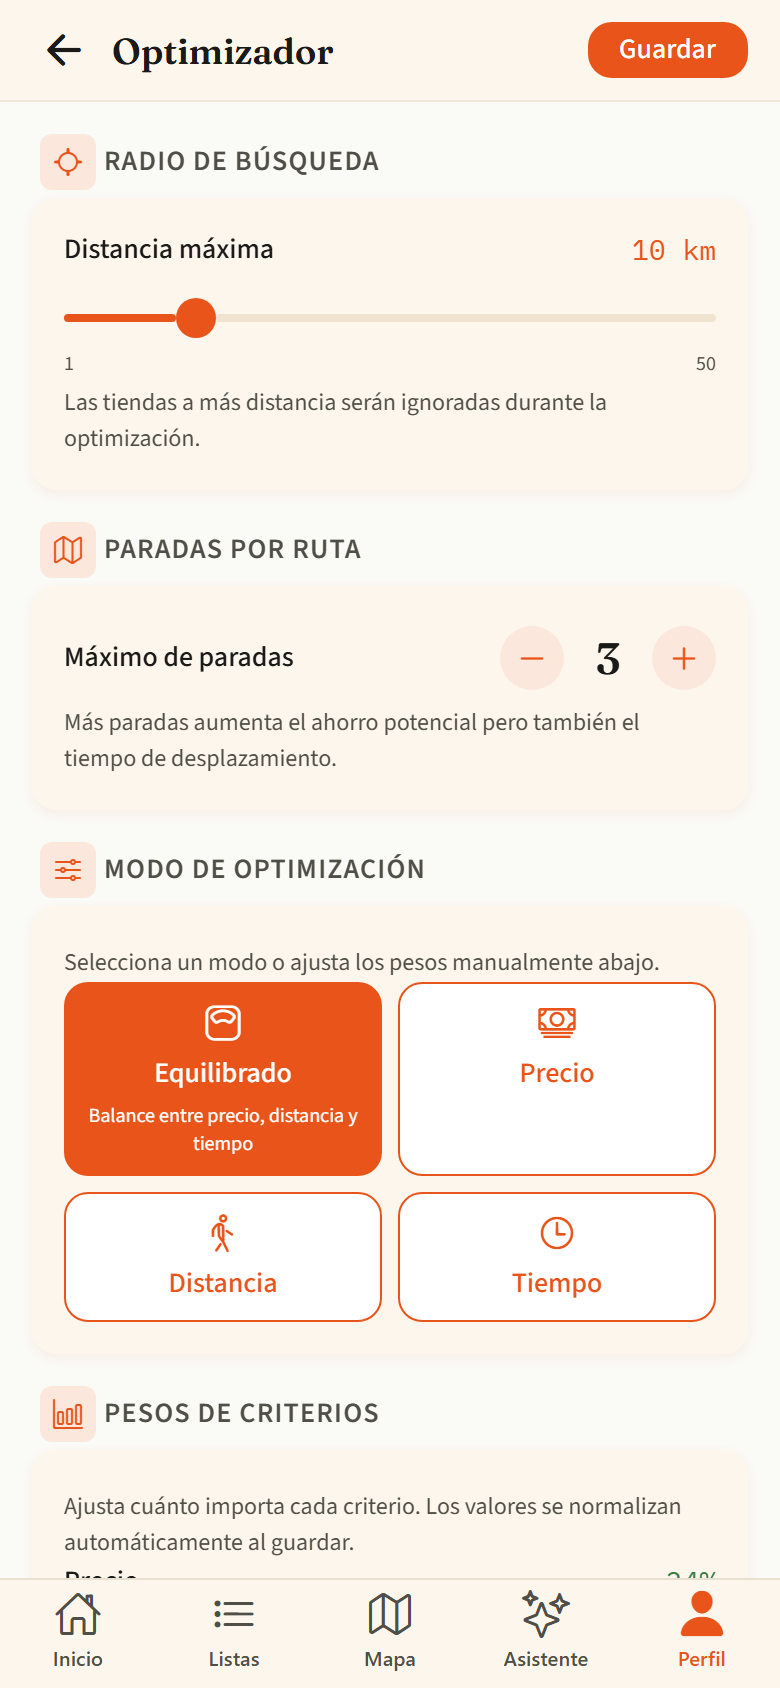
\includegraphics[width=0.30\textwidth]{diagramas/capturas/mobile-config-optimizador.png}
\caption{M\'ovil --- Perfil de usuario (izquierda) y configuraci\'on del optimizador (derecha)}
\label{fig:cap-mobile-perfil-config}
\end{figure}

\begin{figure}[htbp]
\centering
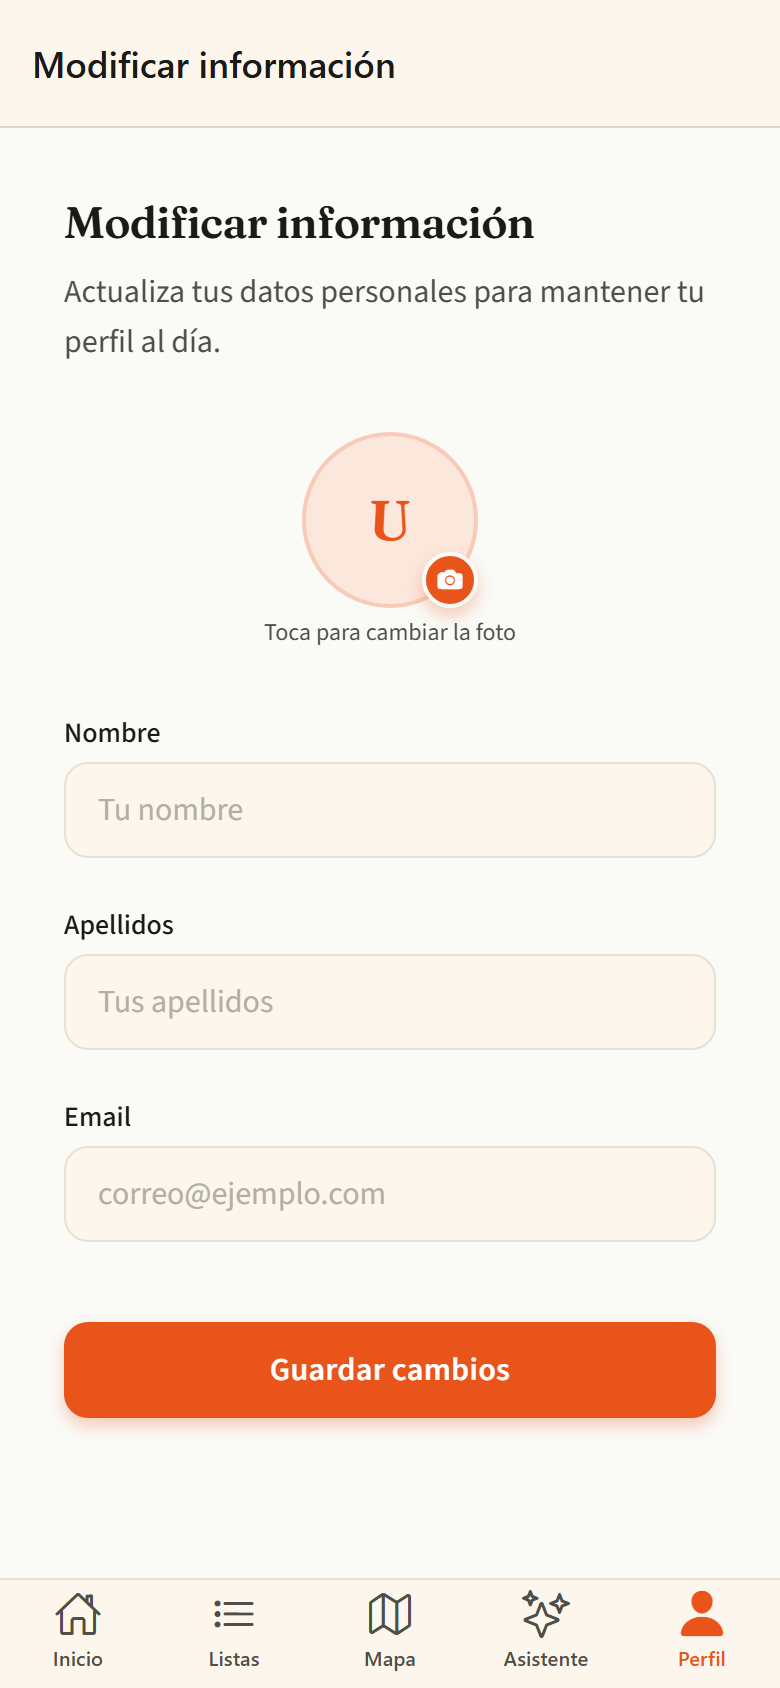
\includegraphics[width=0.30\textwidth]{diagramas/capturas/mobile-editar-perfil.png}
\hfill
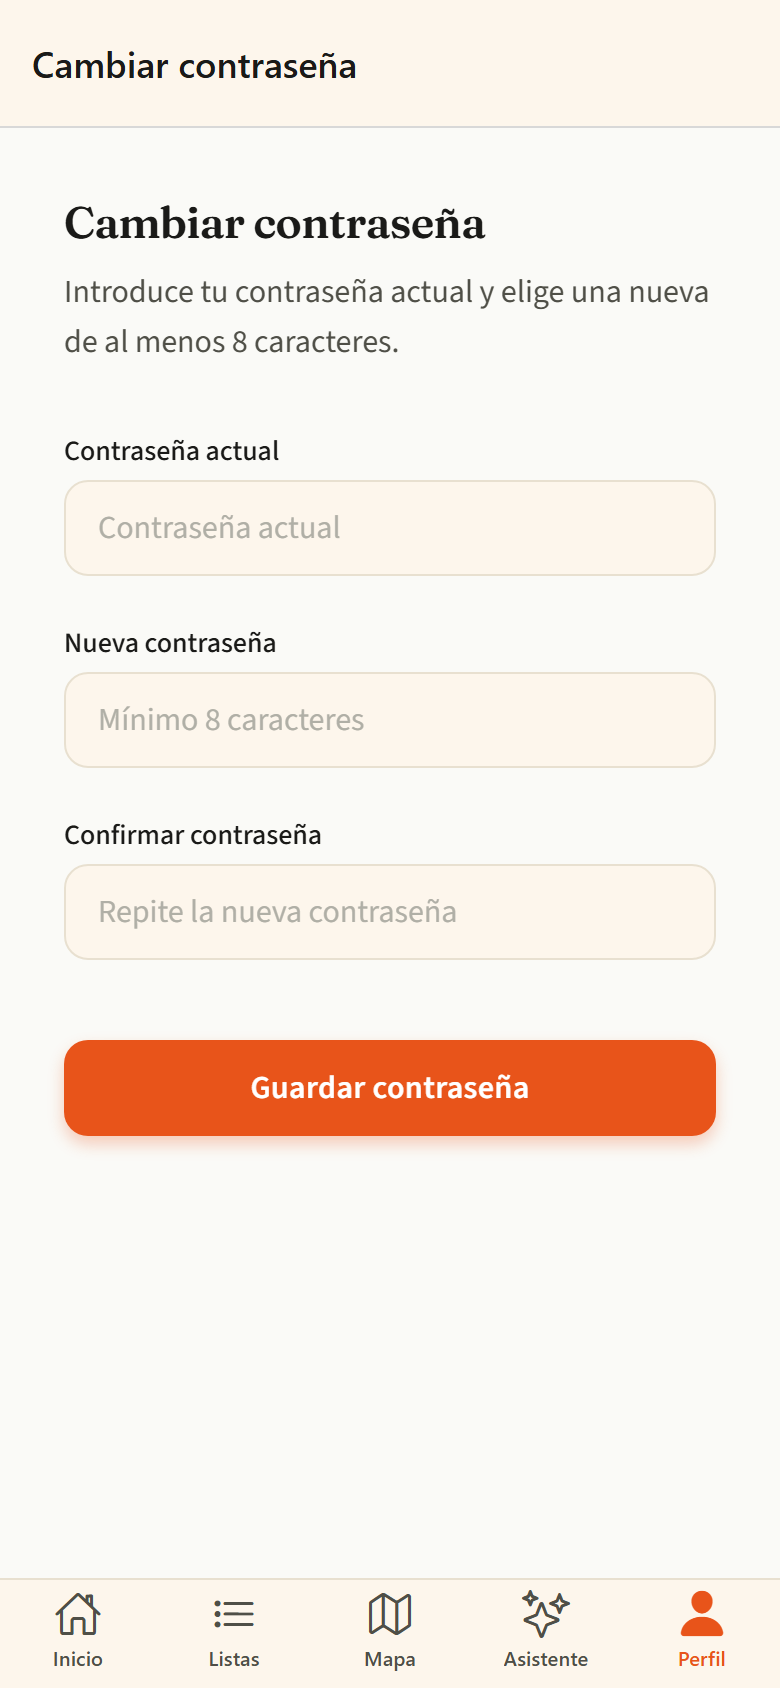
\includegraphics[width=0.30\textwidth]{diagramas/capturas/mobile-cambiar-password.png}
\caption{M\'ovil --- Edici\'on de perfil (izquierda) y cambio de contrase\~na (derecha)}
\label{fig:cap-mobile-editar-password}
\end{figure}

\clearpage

\subsection{Aplicaci\'on web (usuario)}\label{subsec:galeria-web}

\begin{figure}[htbp]
\centering
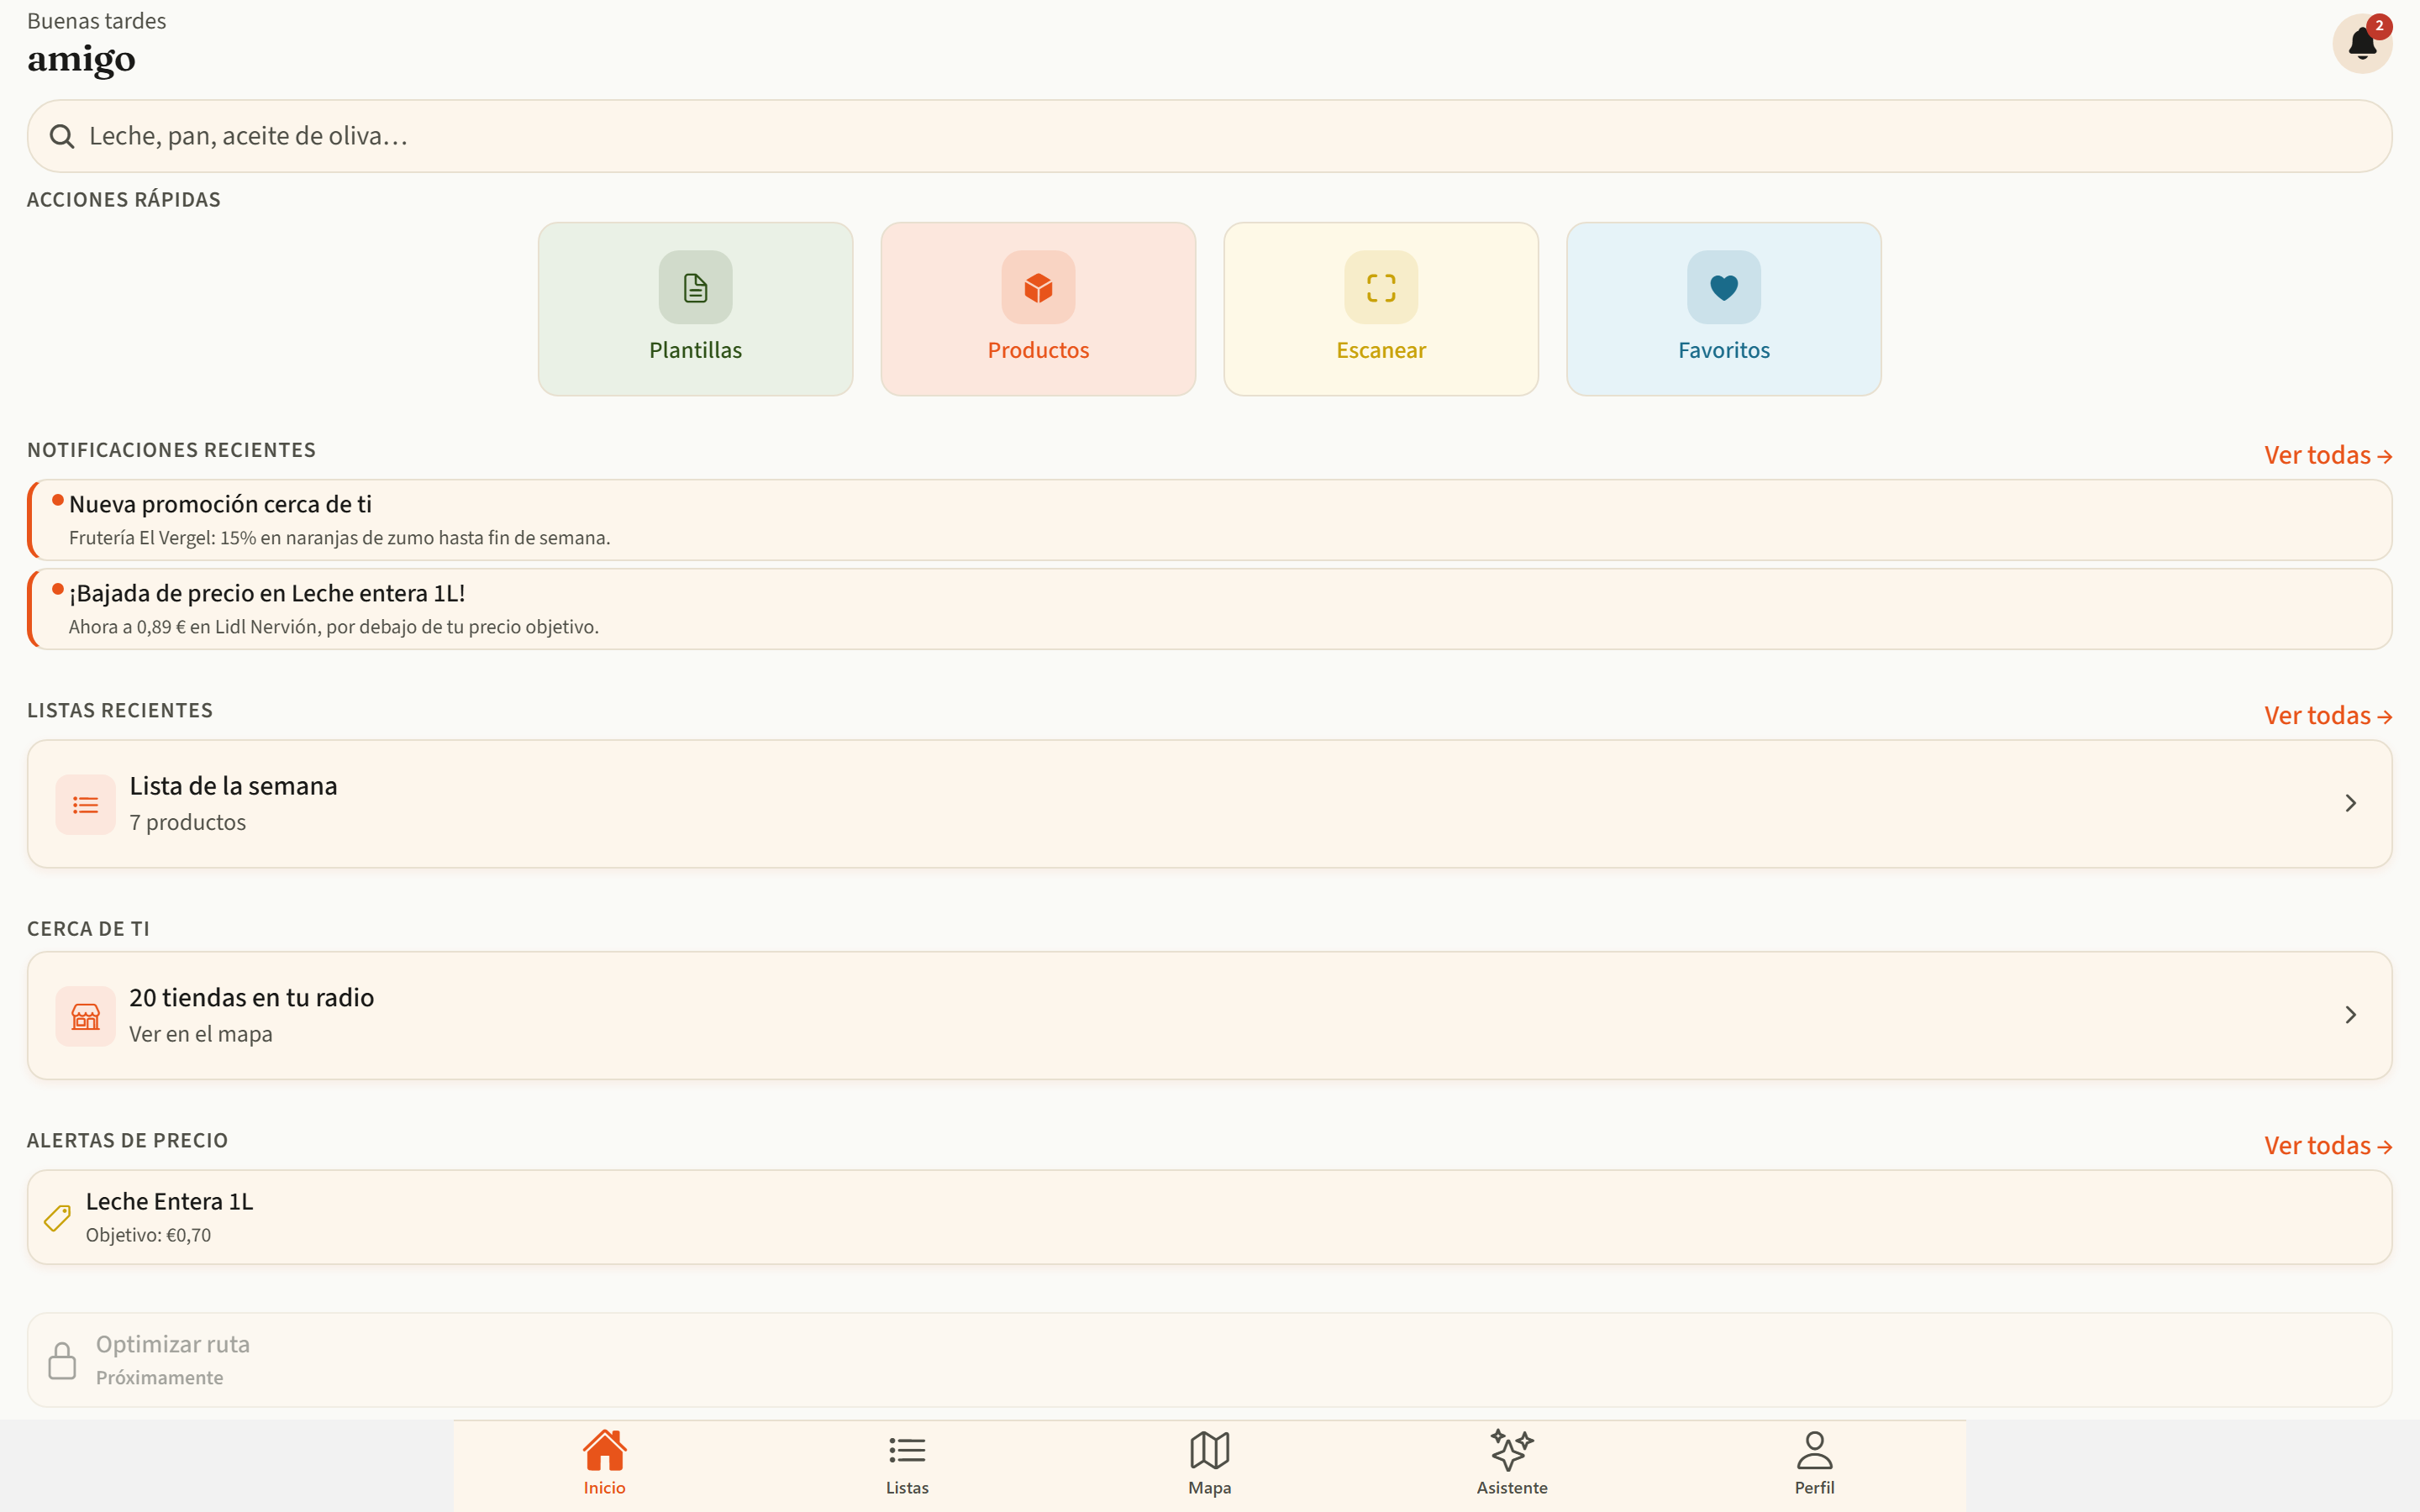
\includegraphics[width=0.46\textwidth]{diagramas/capturas/web-home.png}
\hfill
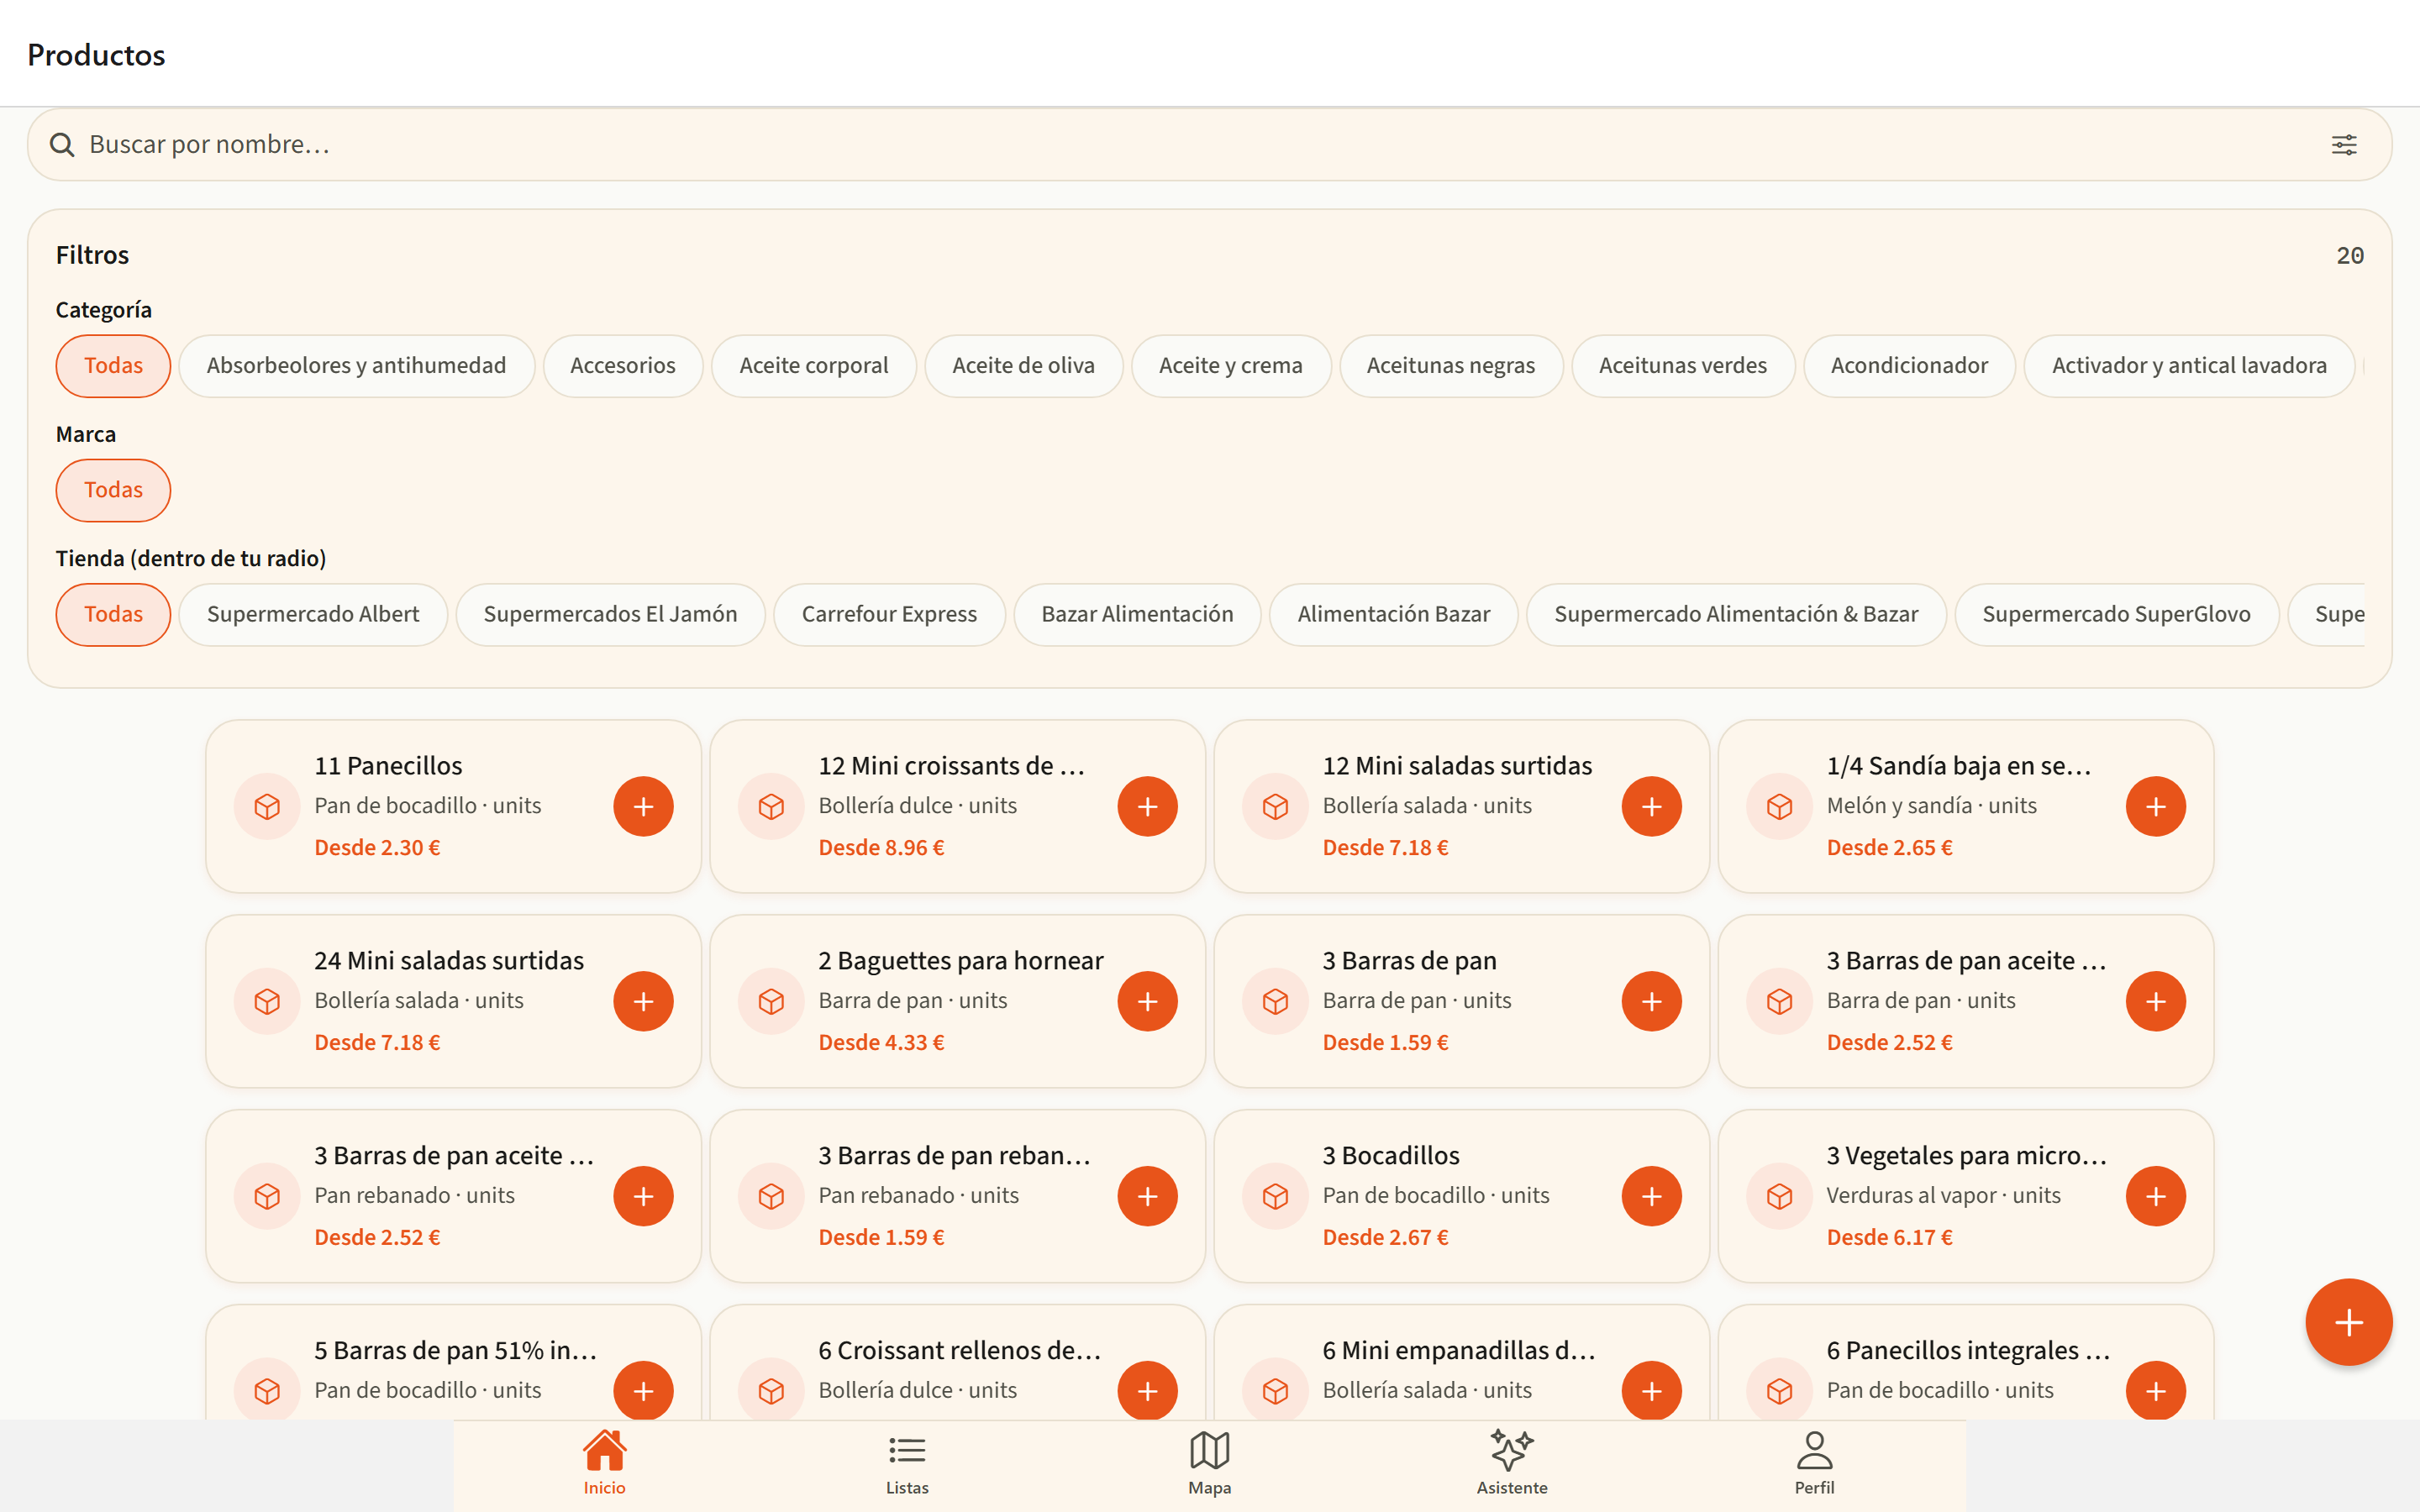
\includegraphics[width=0.46\textwidth]{diagramas/capturas/web-catalogo.png}
\caption{Web --- Pantalla principal con accesos horizontales (izquierda) y cat\'alogo en rejilla
multicolumna con \texttt{Cmd/Ctrl+K} (derecha)}
\label{fig:cap-web-home-catalogo}
\end{figure}

\begin{figure}[htbp]
\centering
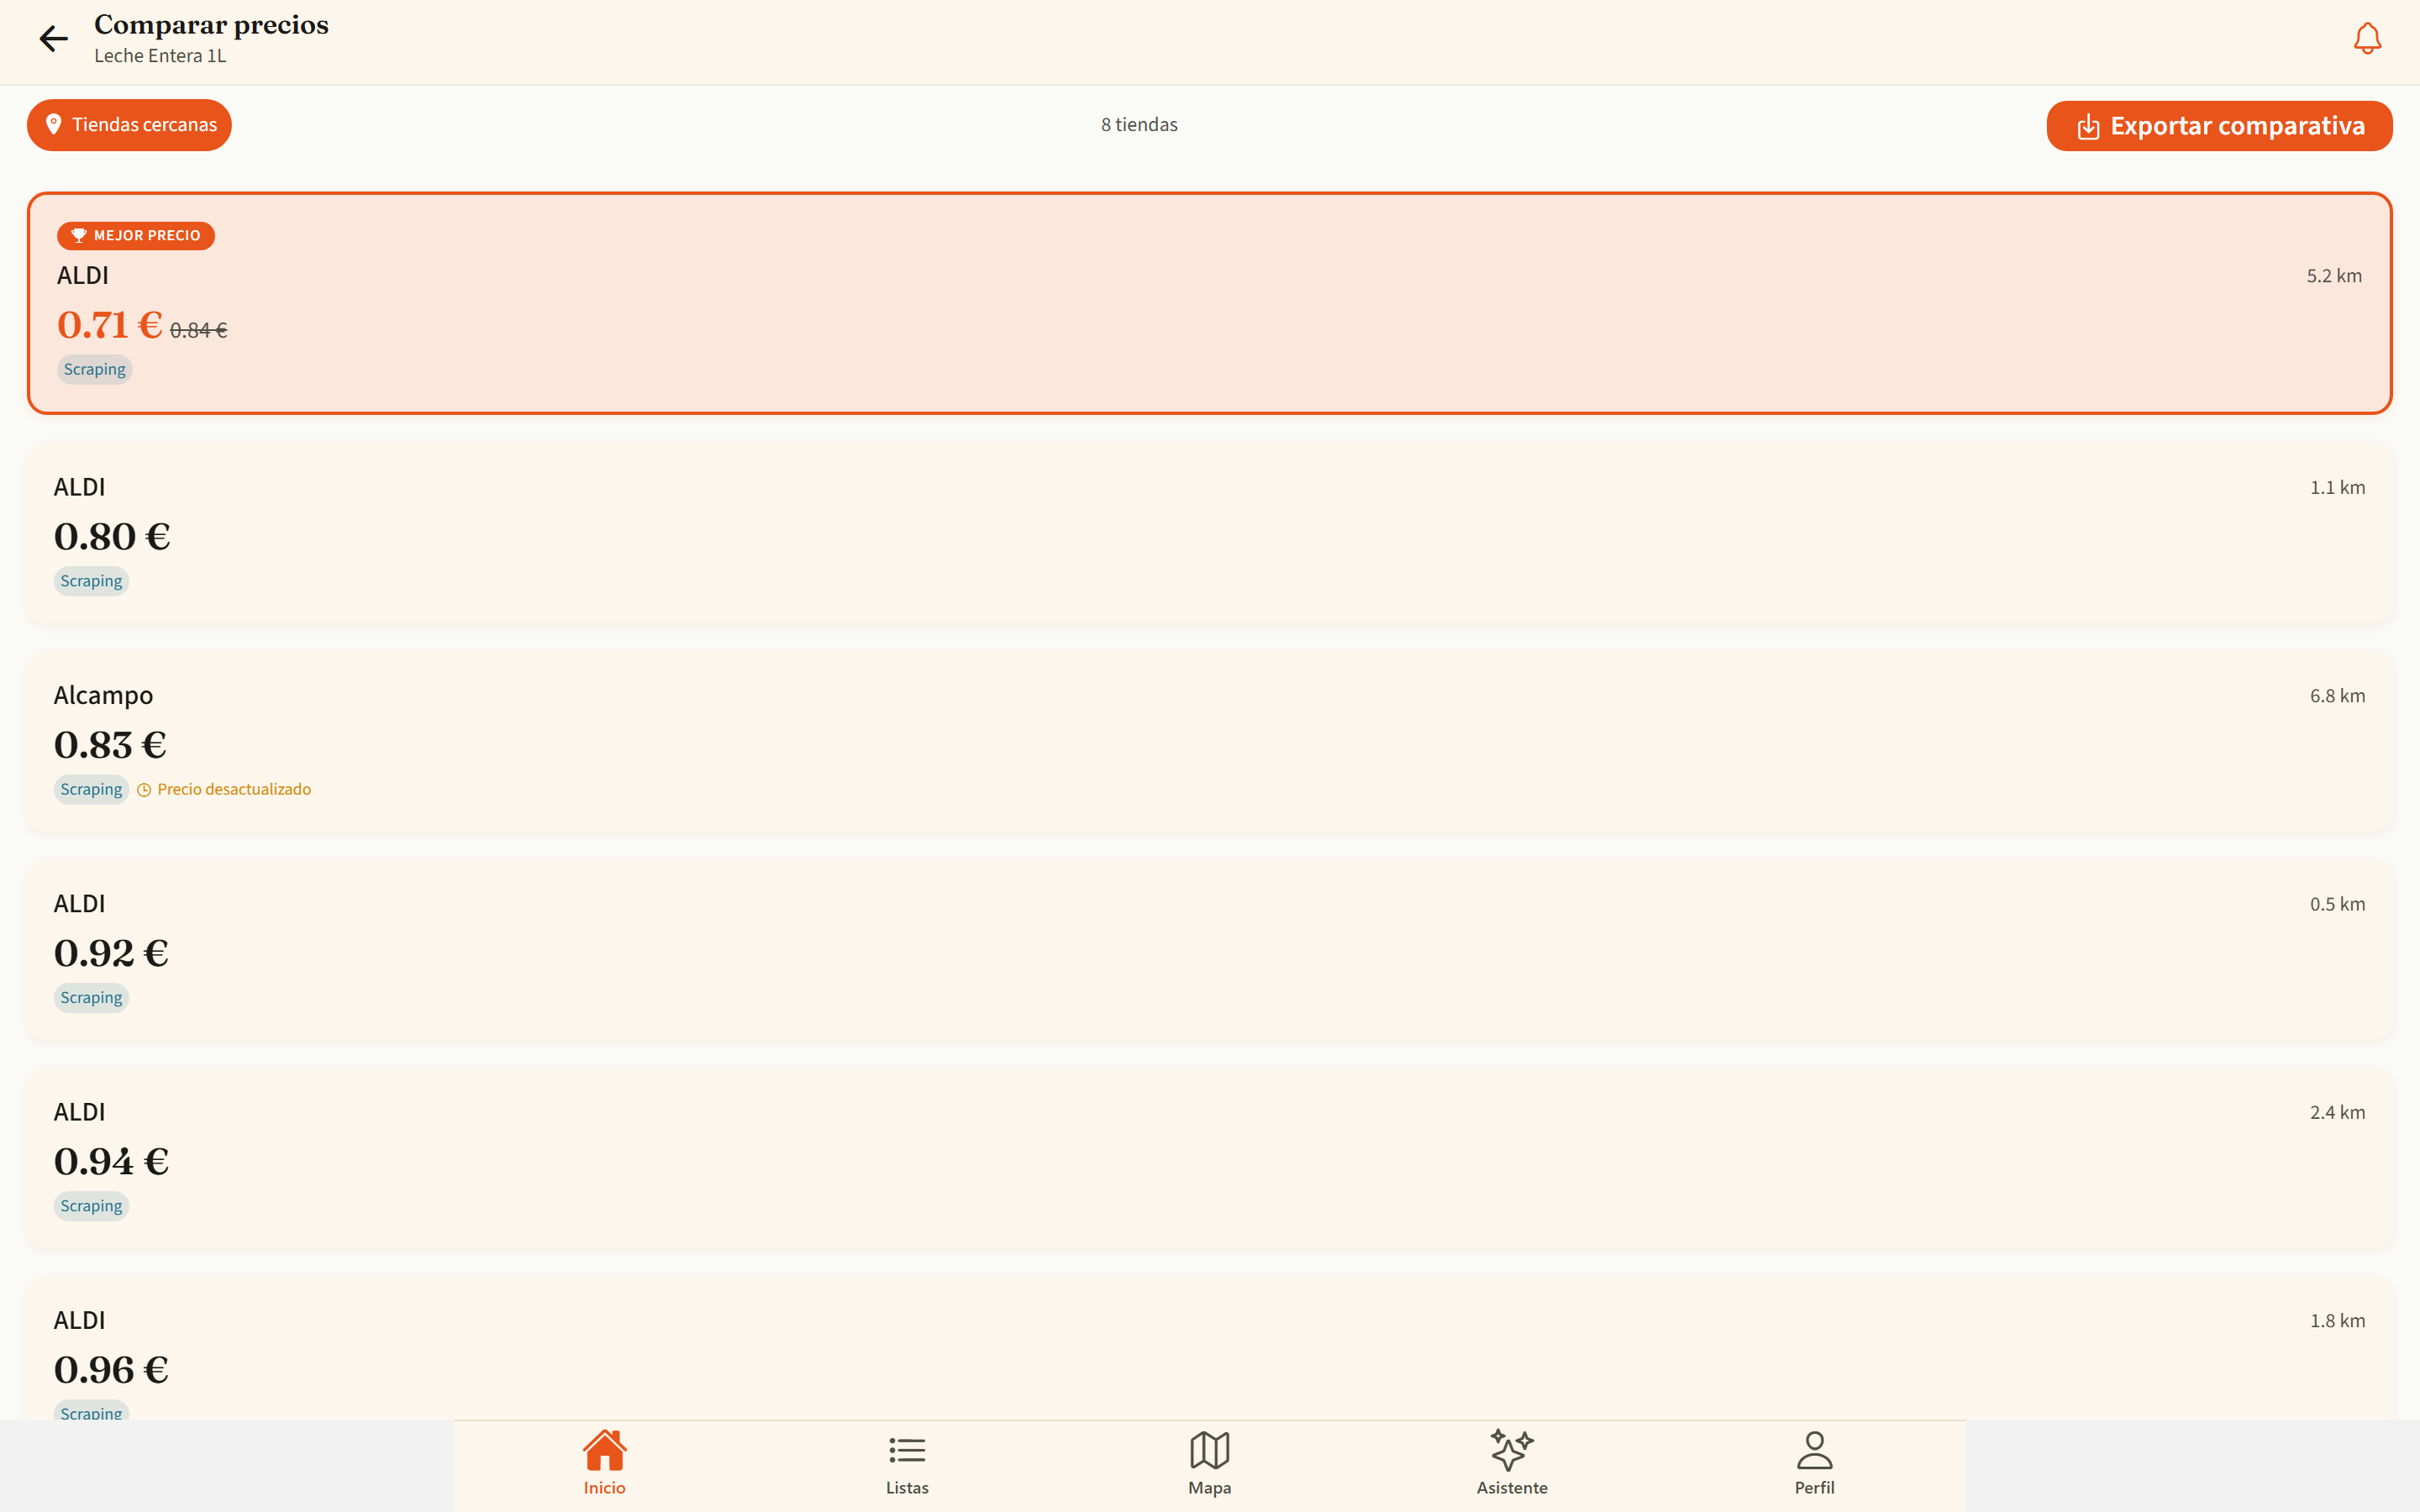
\includegraphics[width=0.46\textwidth]{diagramas/capturas/web-comparativa.png}
\hfill
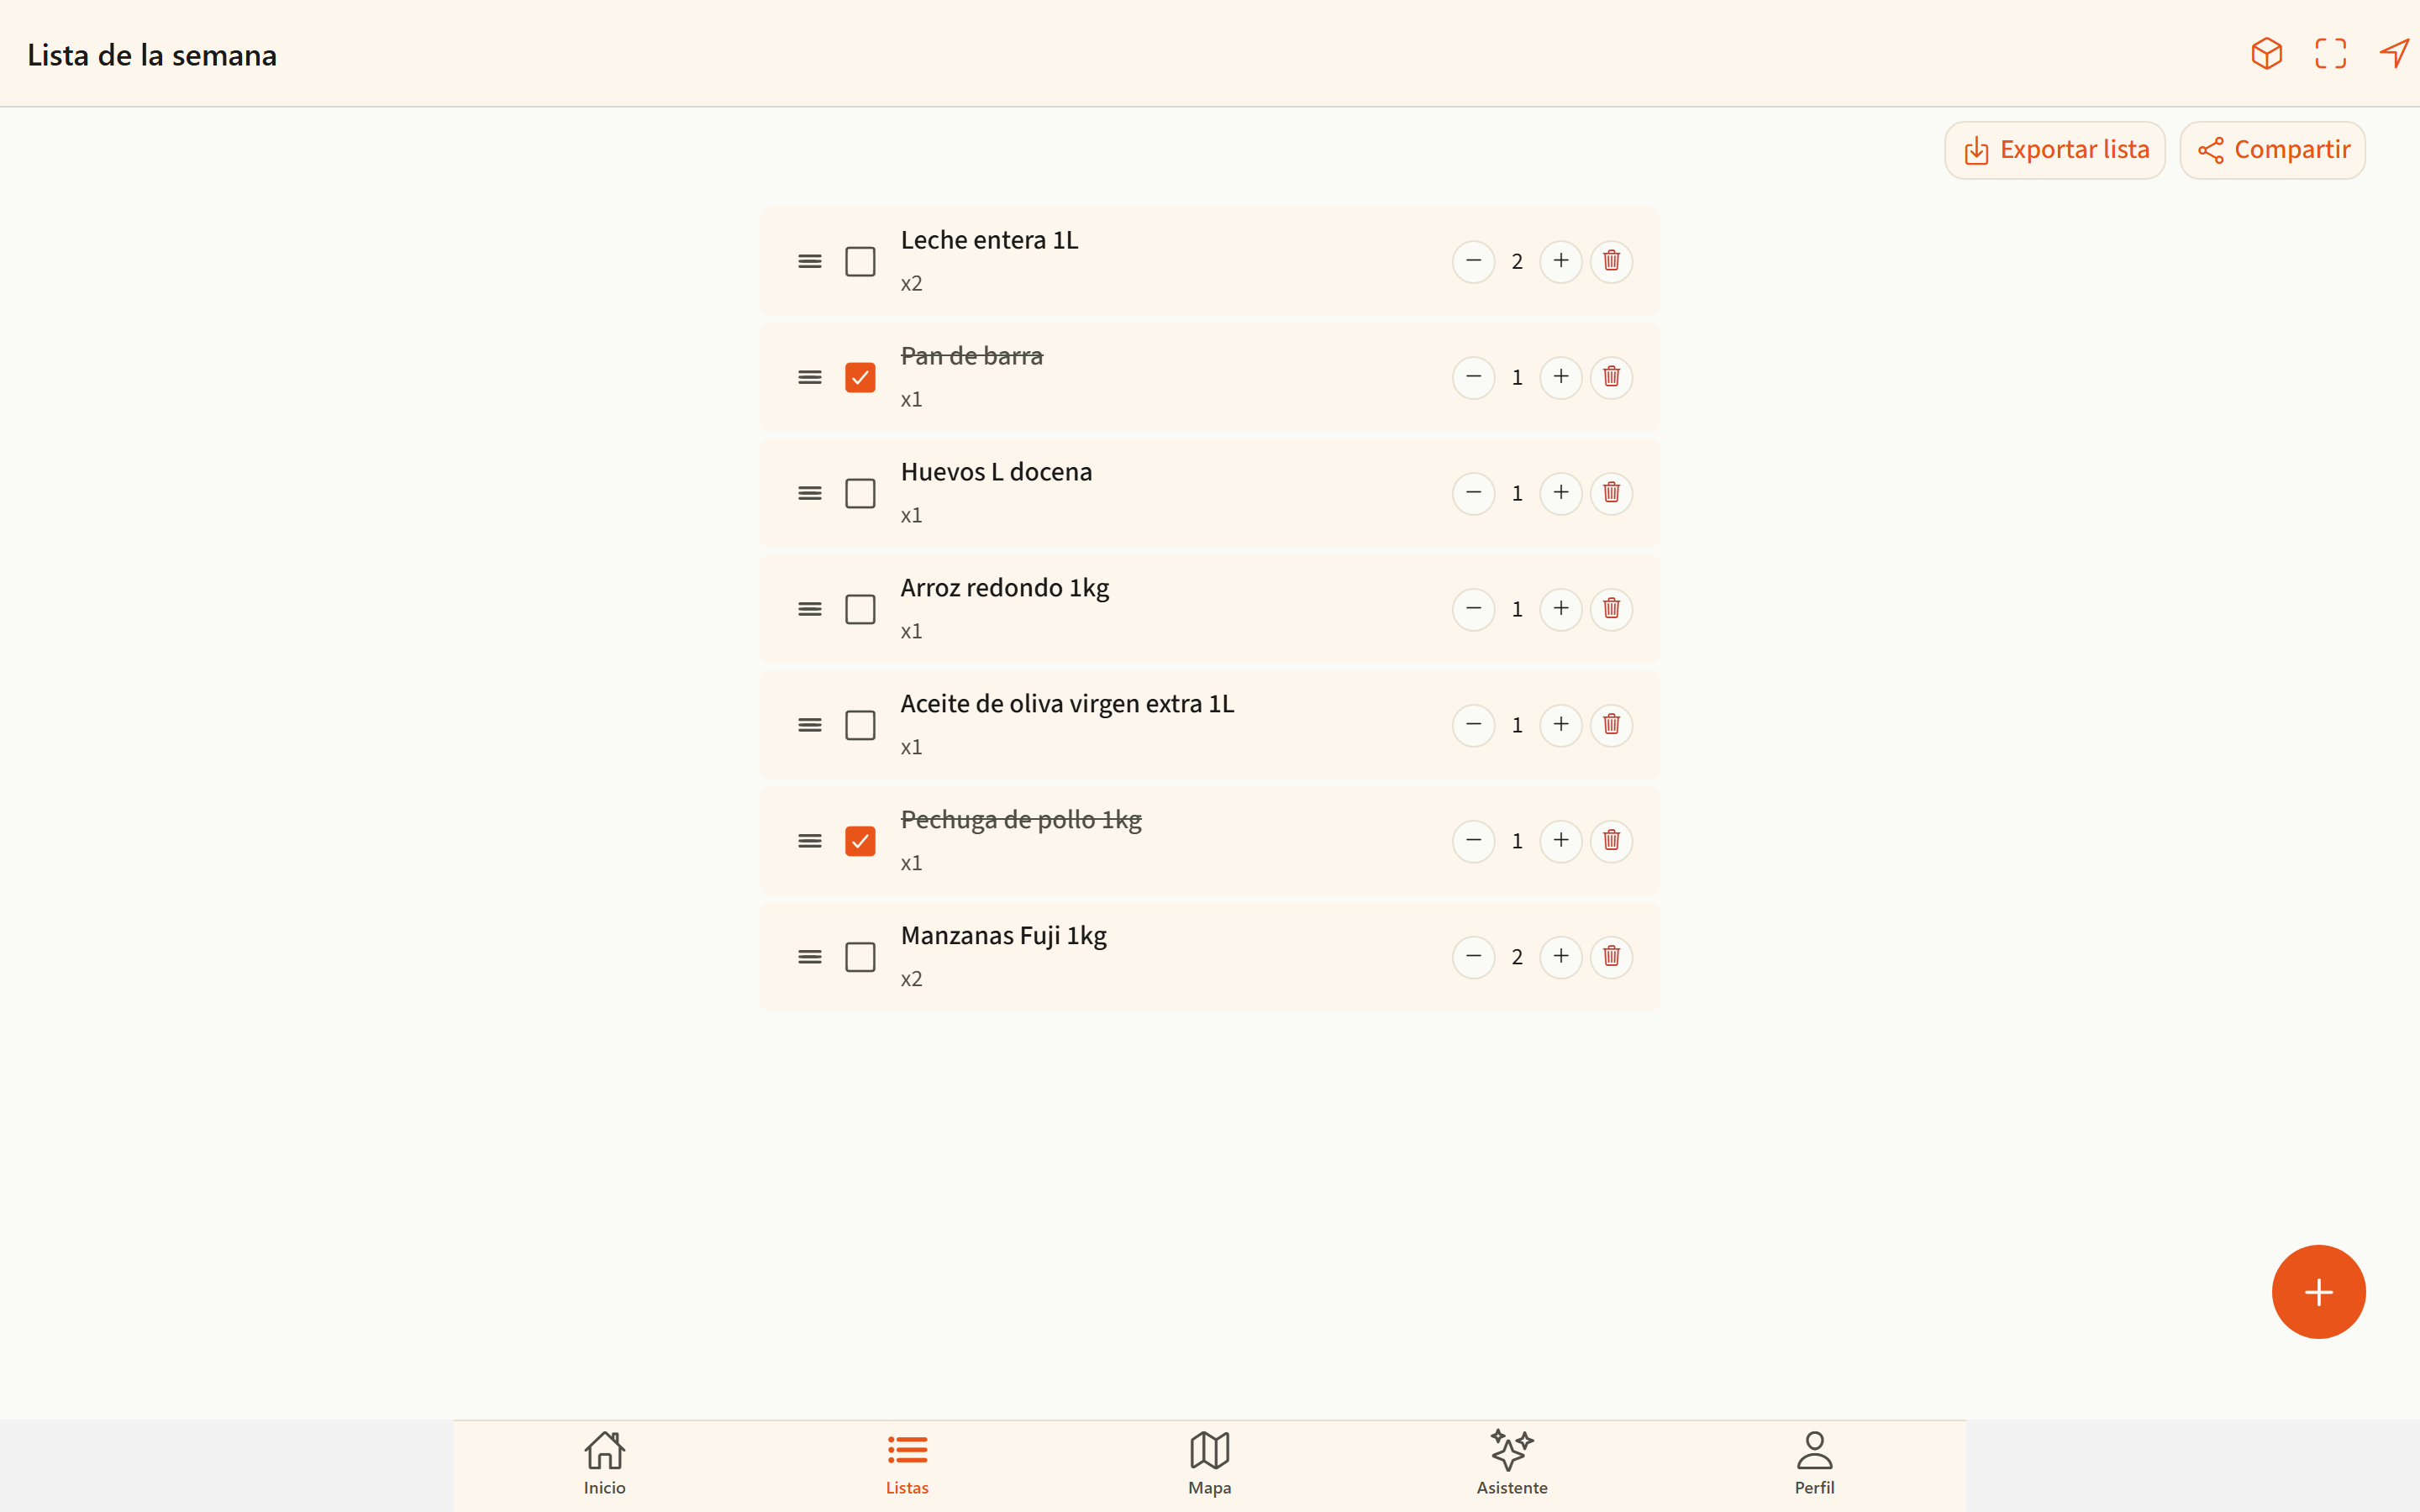
\includegraphics[width=0.46\textwidth]{diagramas/capturas/web-lista-detalle.png}
\caption{Web --- Comparativa de precios con cabecera fija y exportaci\'on CSV (izquierda) y detalle
de lista con reordenado \emph{drag-and-drop} y exportaci\'on (derecha)}
\label{fig:cap-web-comparativa-lista}
\end{figure}

\begin{figure}[htbp]
\centering
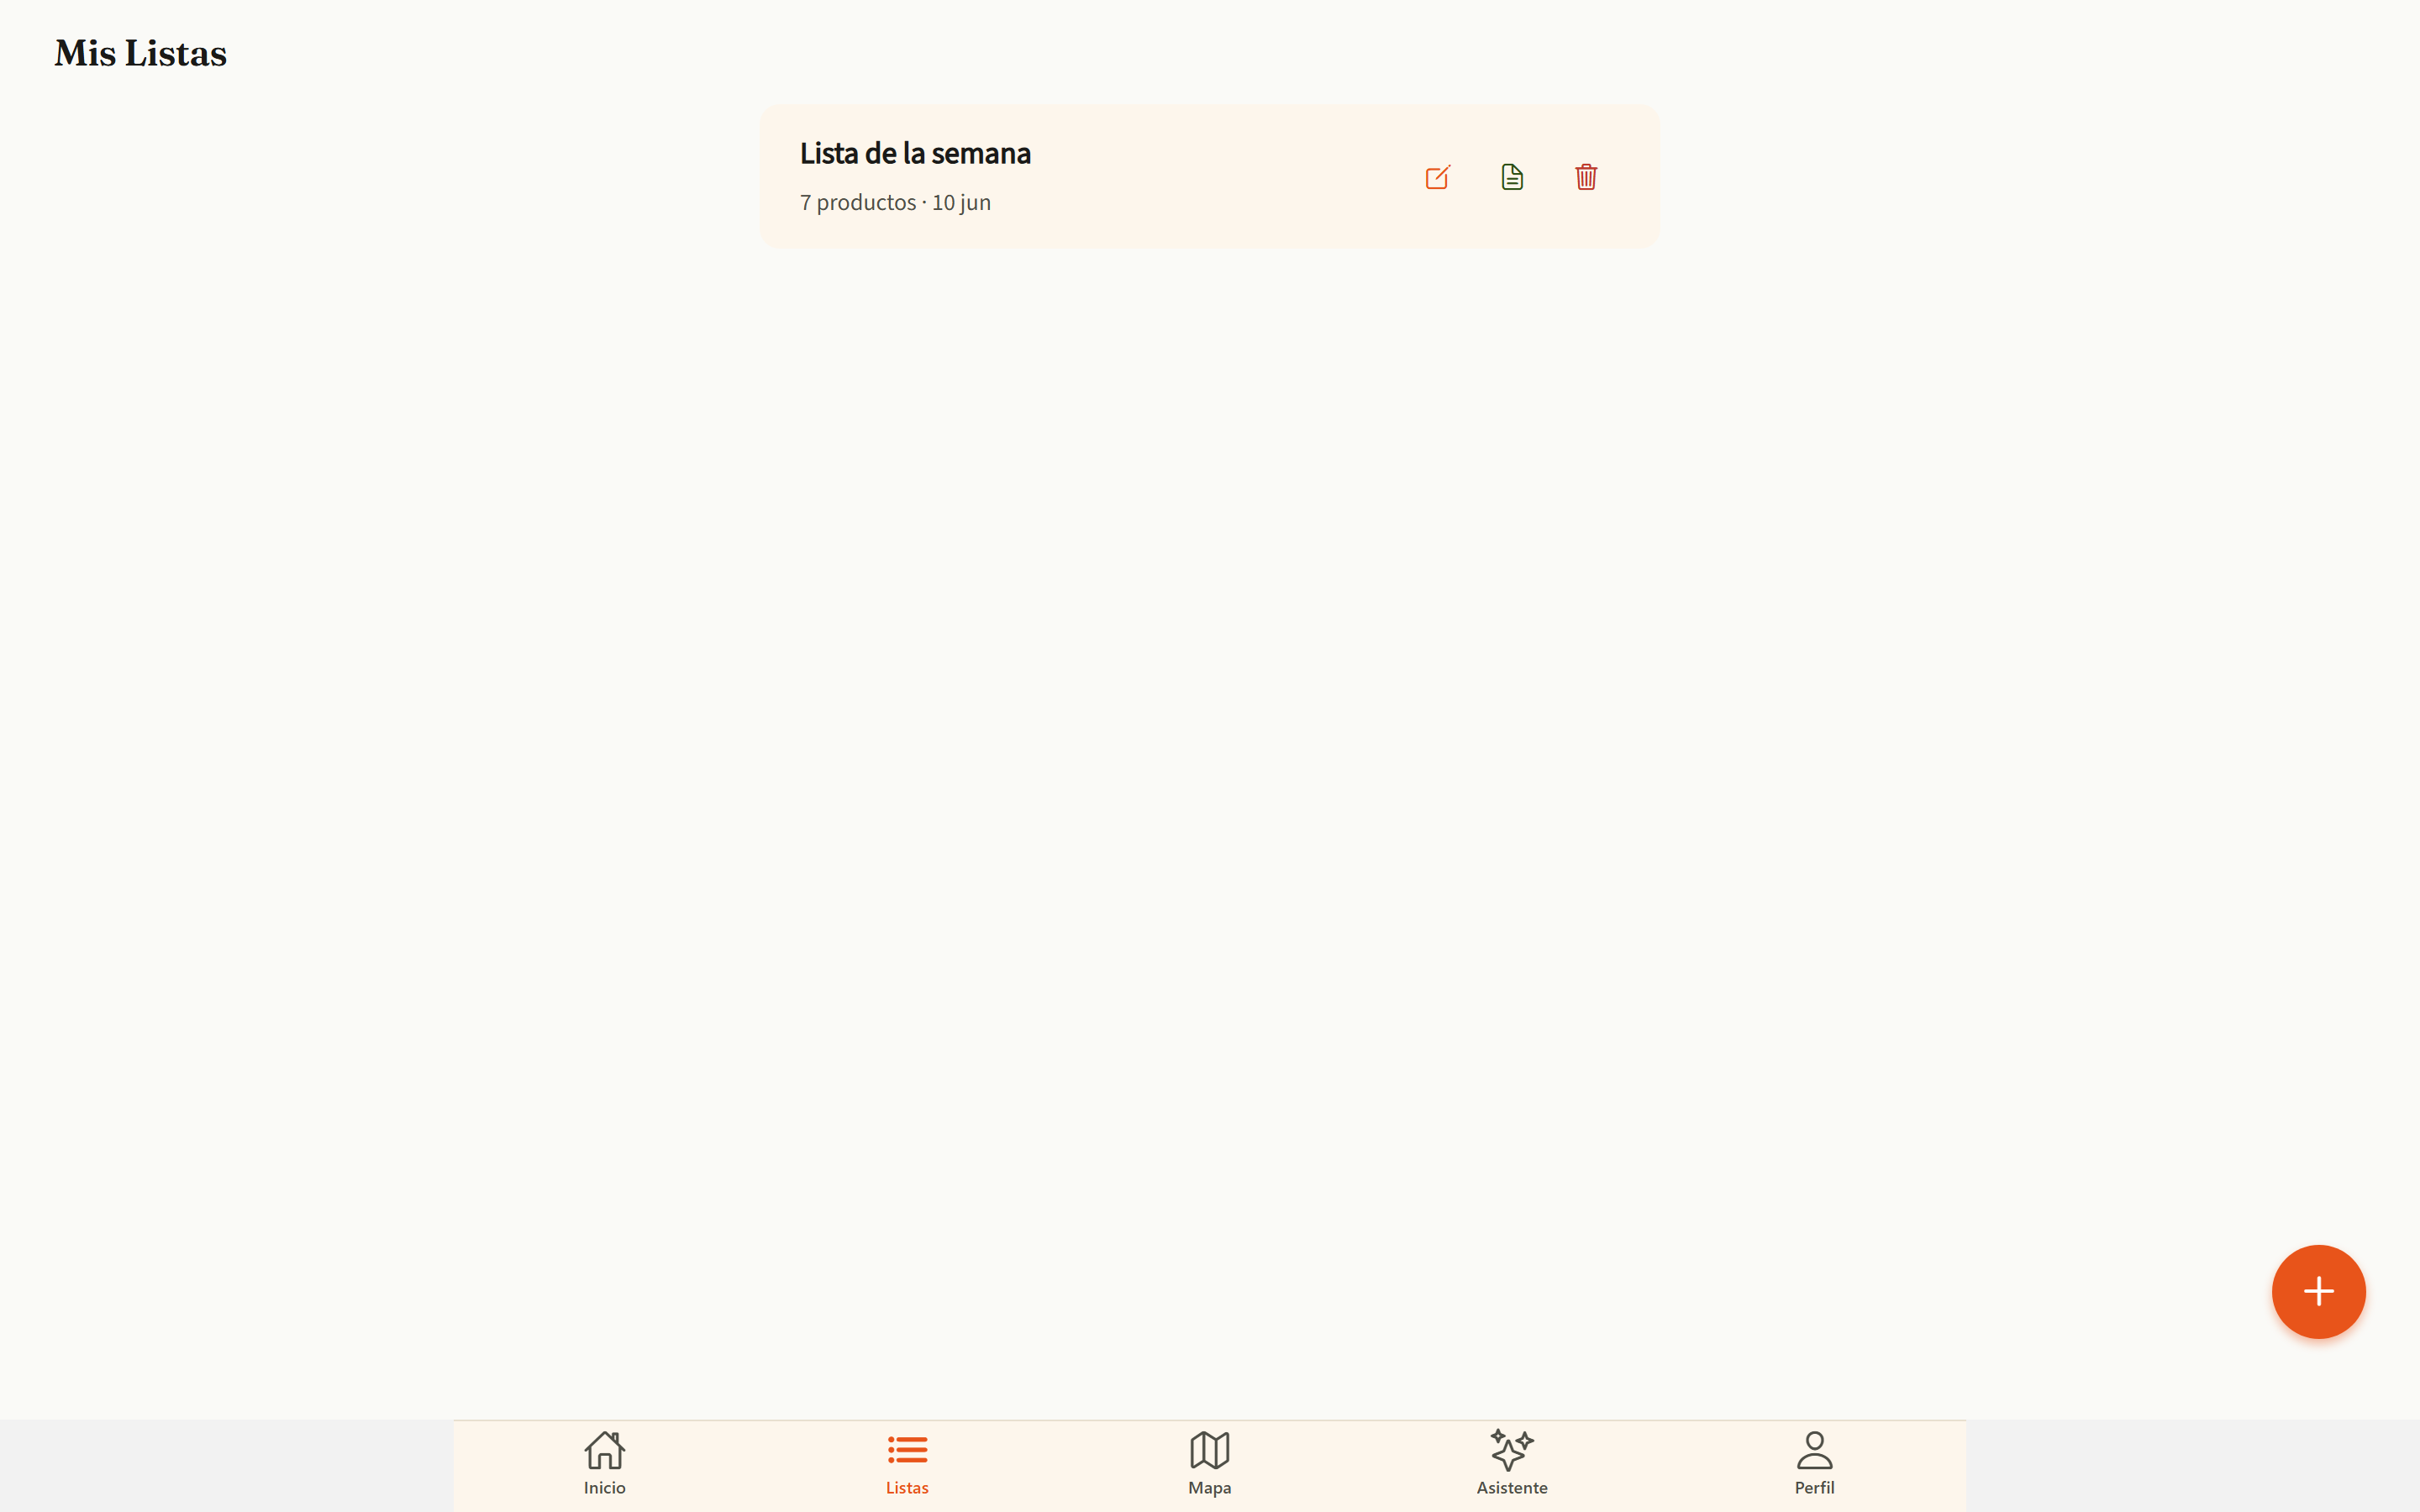
\includegraphics[width=0.46\textwidth]{diagramas/capturas/web-listas.png}
\hfill
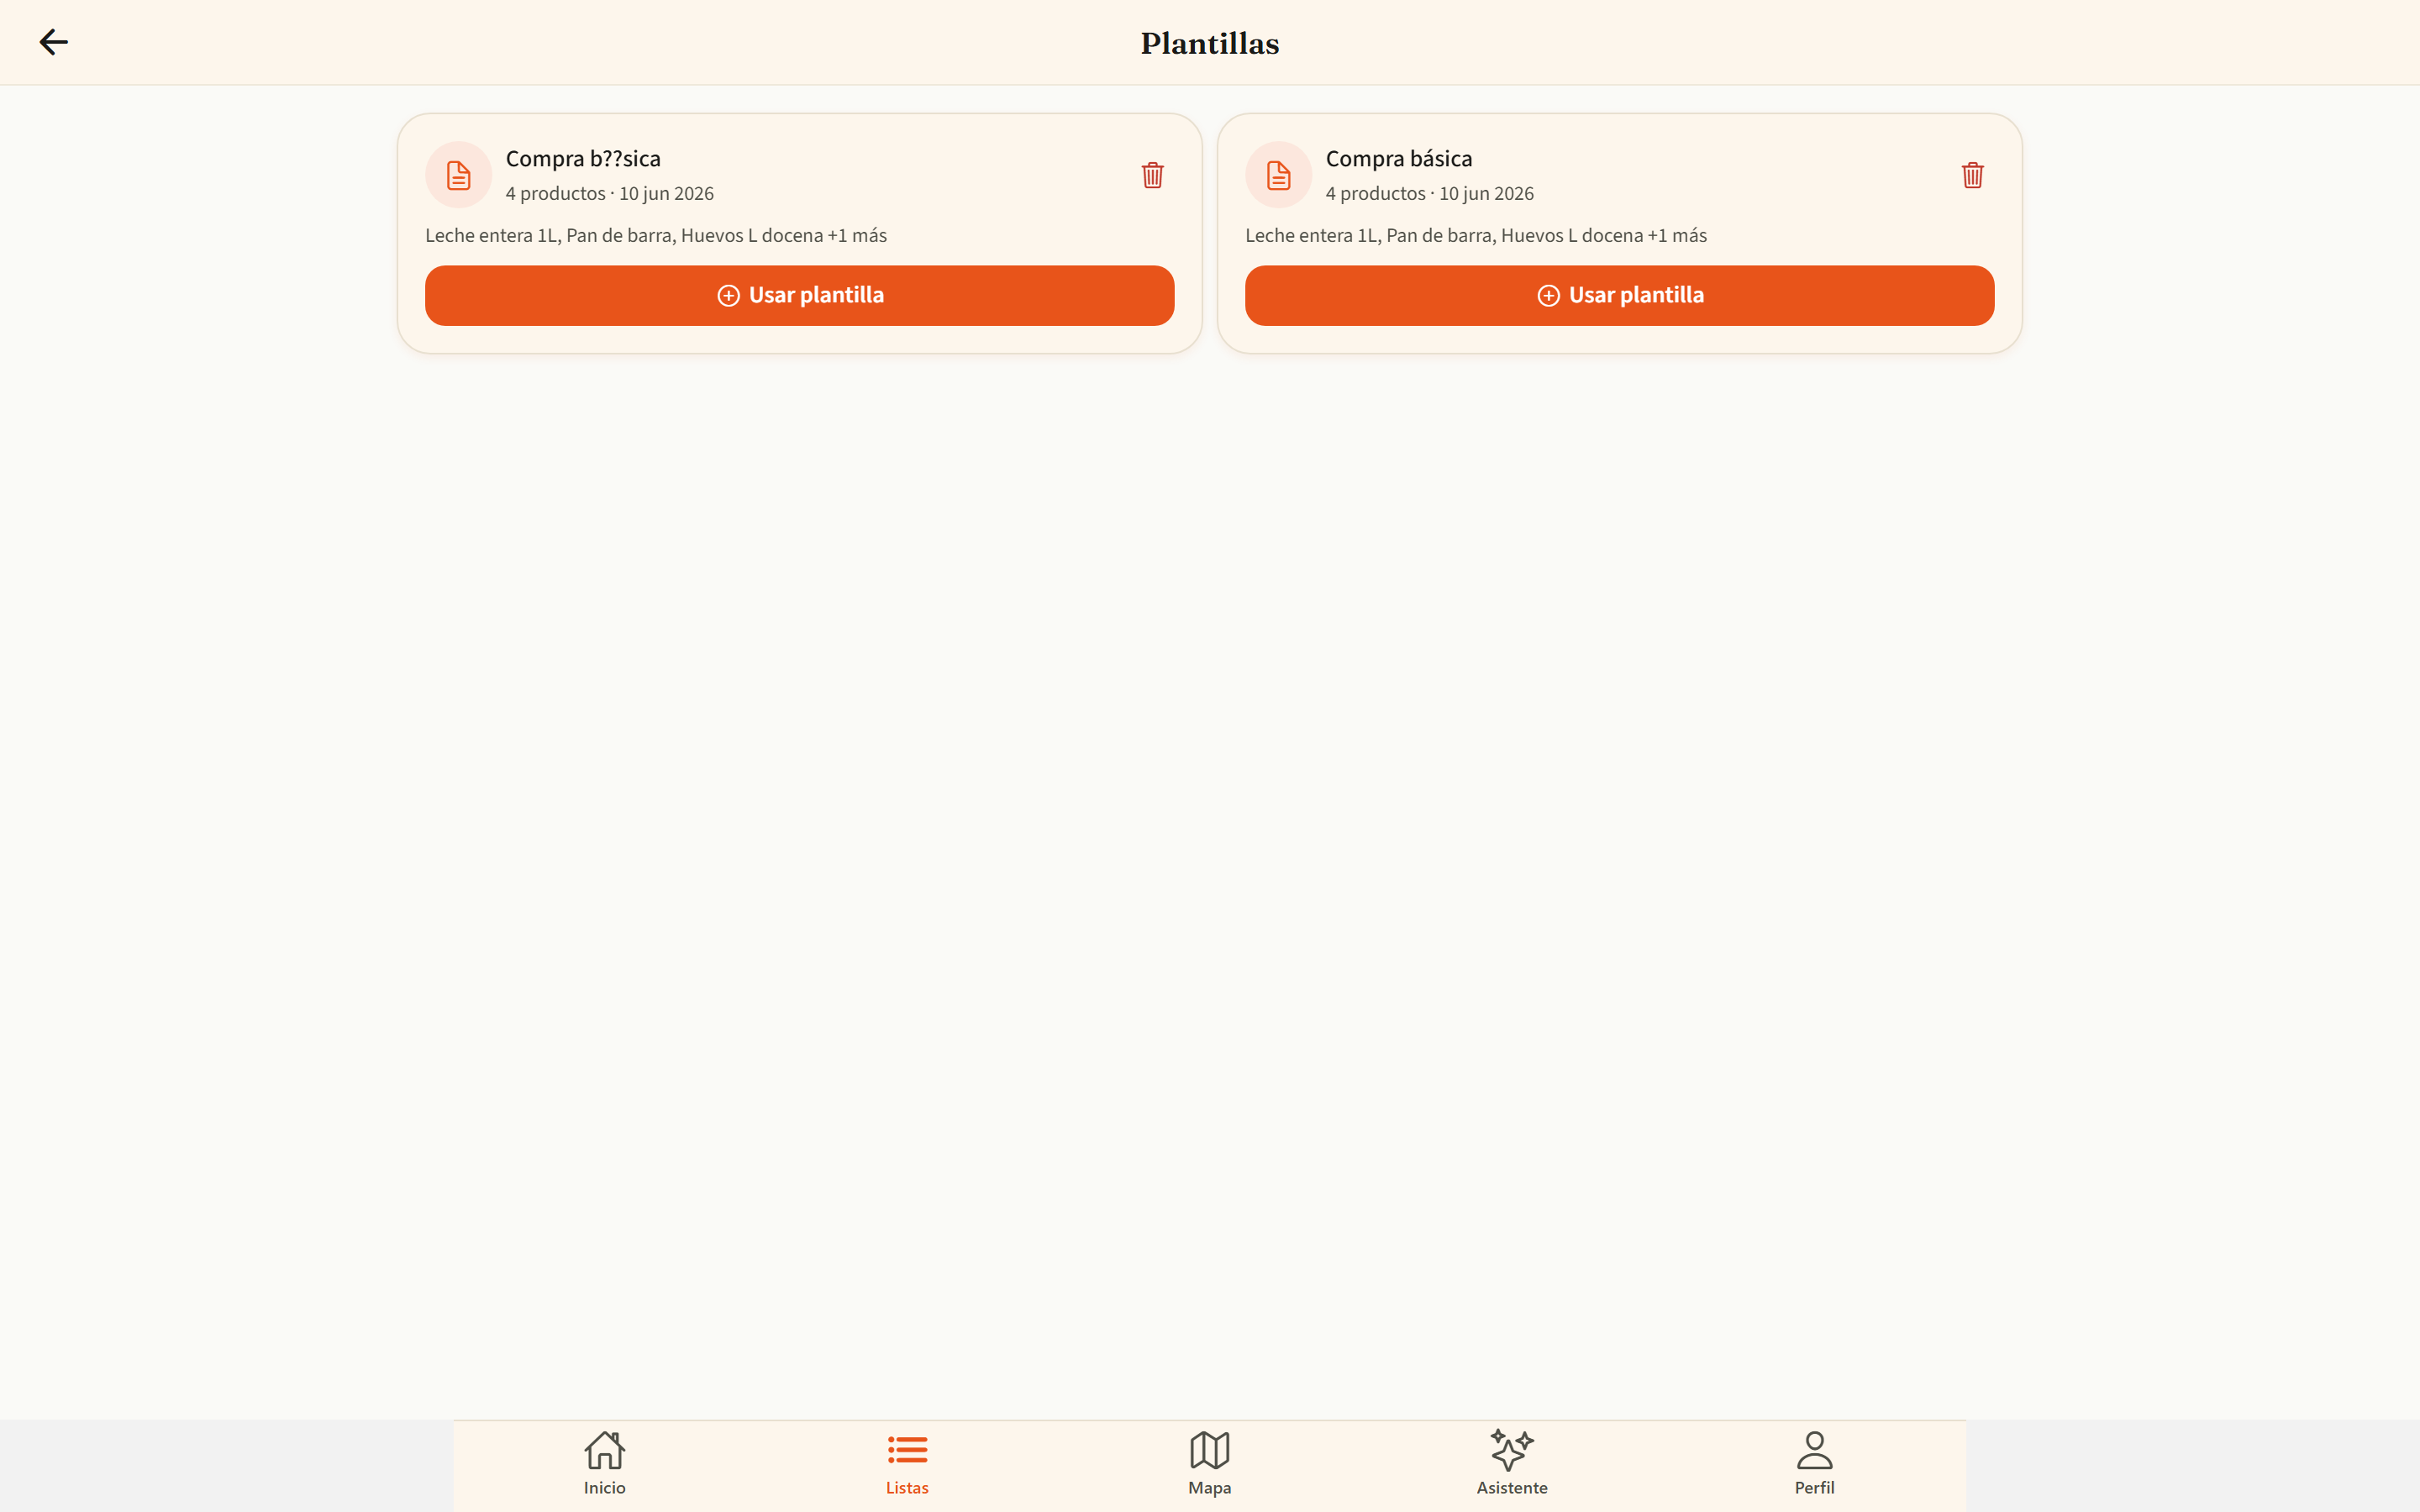
\includegraphics[width=0.46\textwidth]{diagramas/capturas/web-plantillas.png}
\caption{Web --- Listas (izquierda) y plantillas (derecha) con rejilla responsive}
\label{fig:cap-web-listas-plantillas}
\end{figure}

\begin{figure}[htbp]
\centering
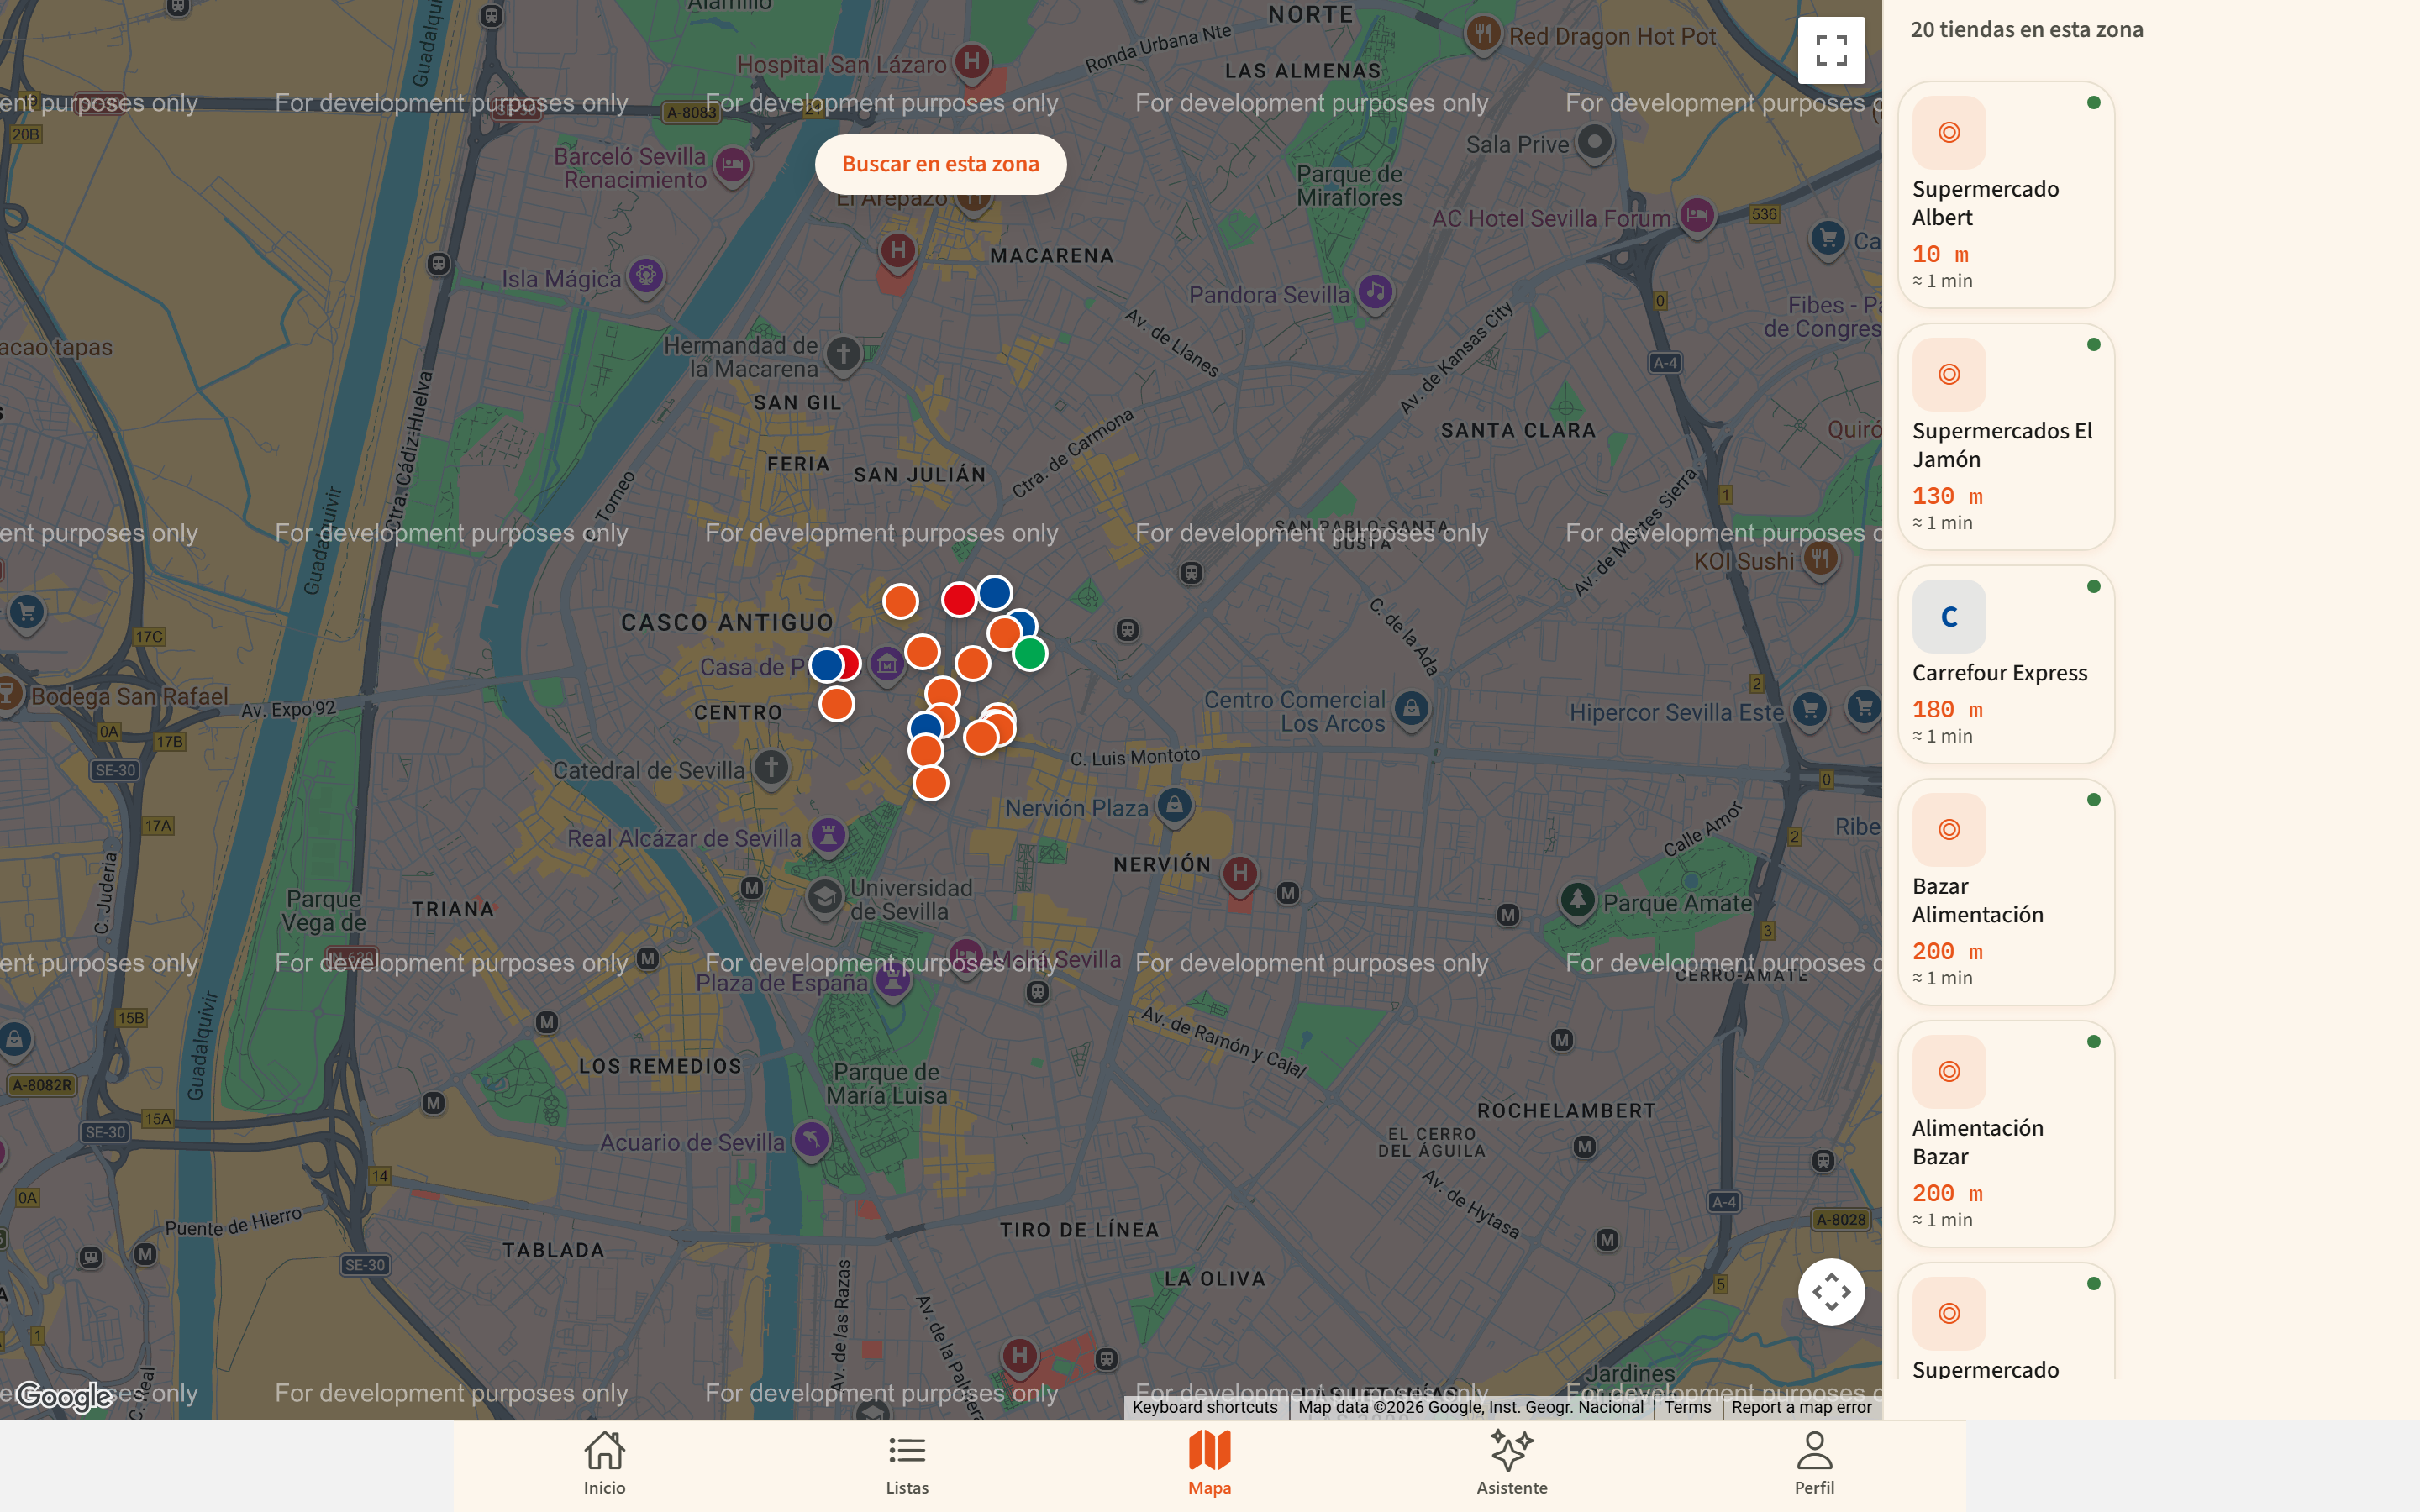
\includegraphics[width=0.46\textwidth]{diagramas/capturas/web-mapa.png}
\hfill
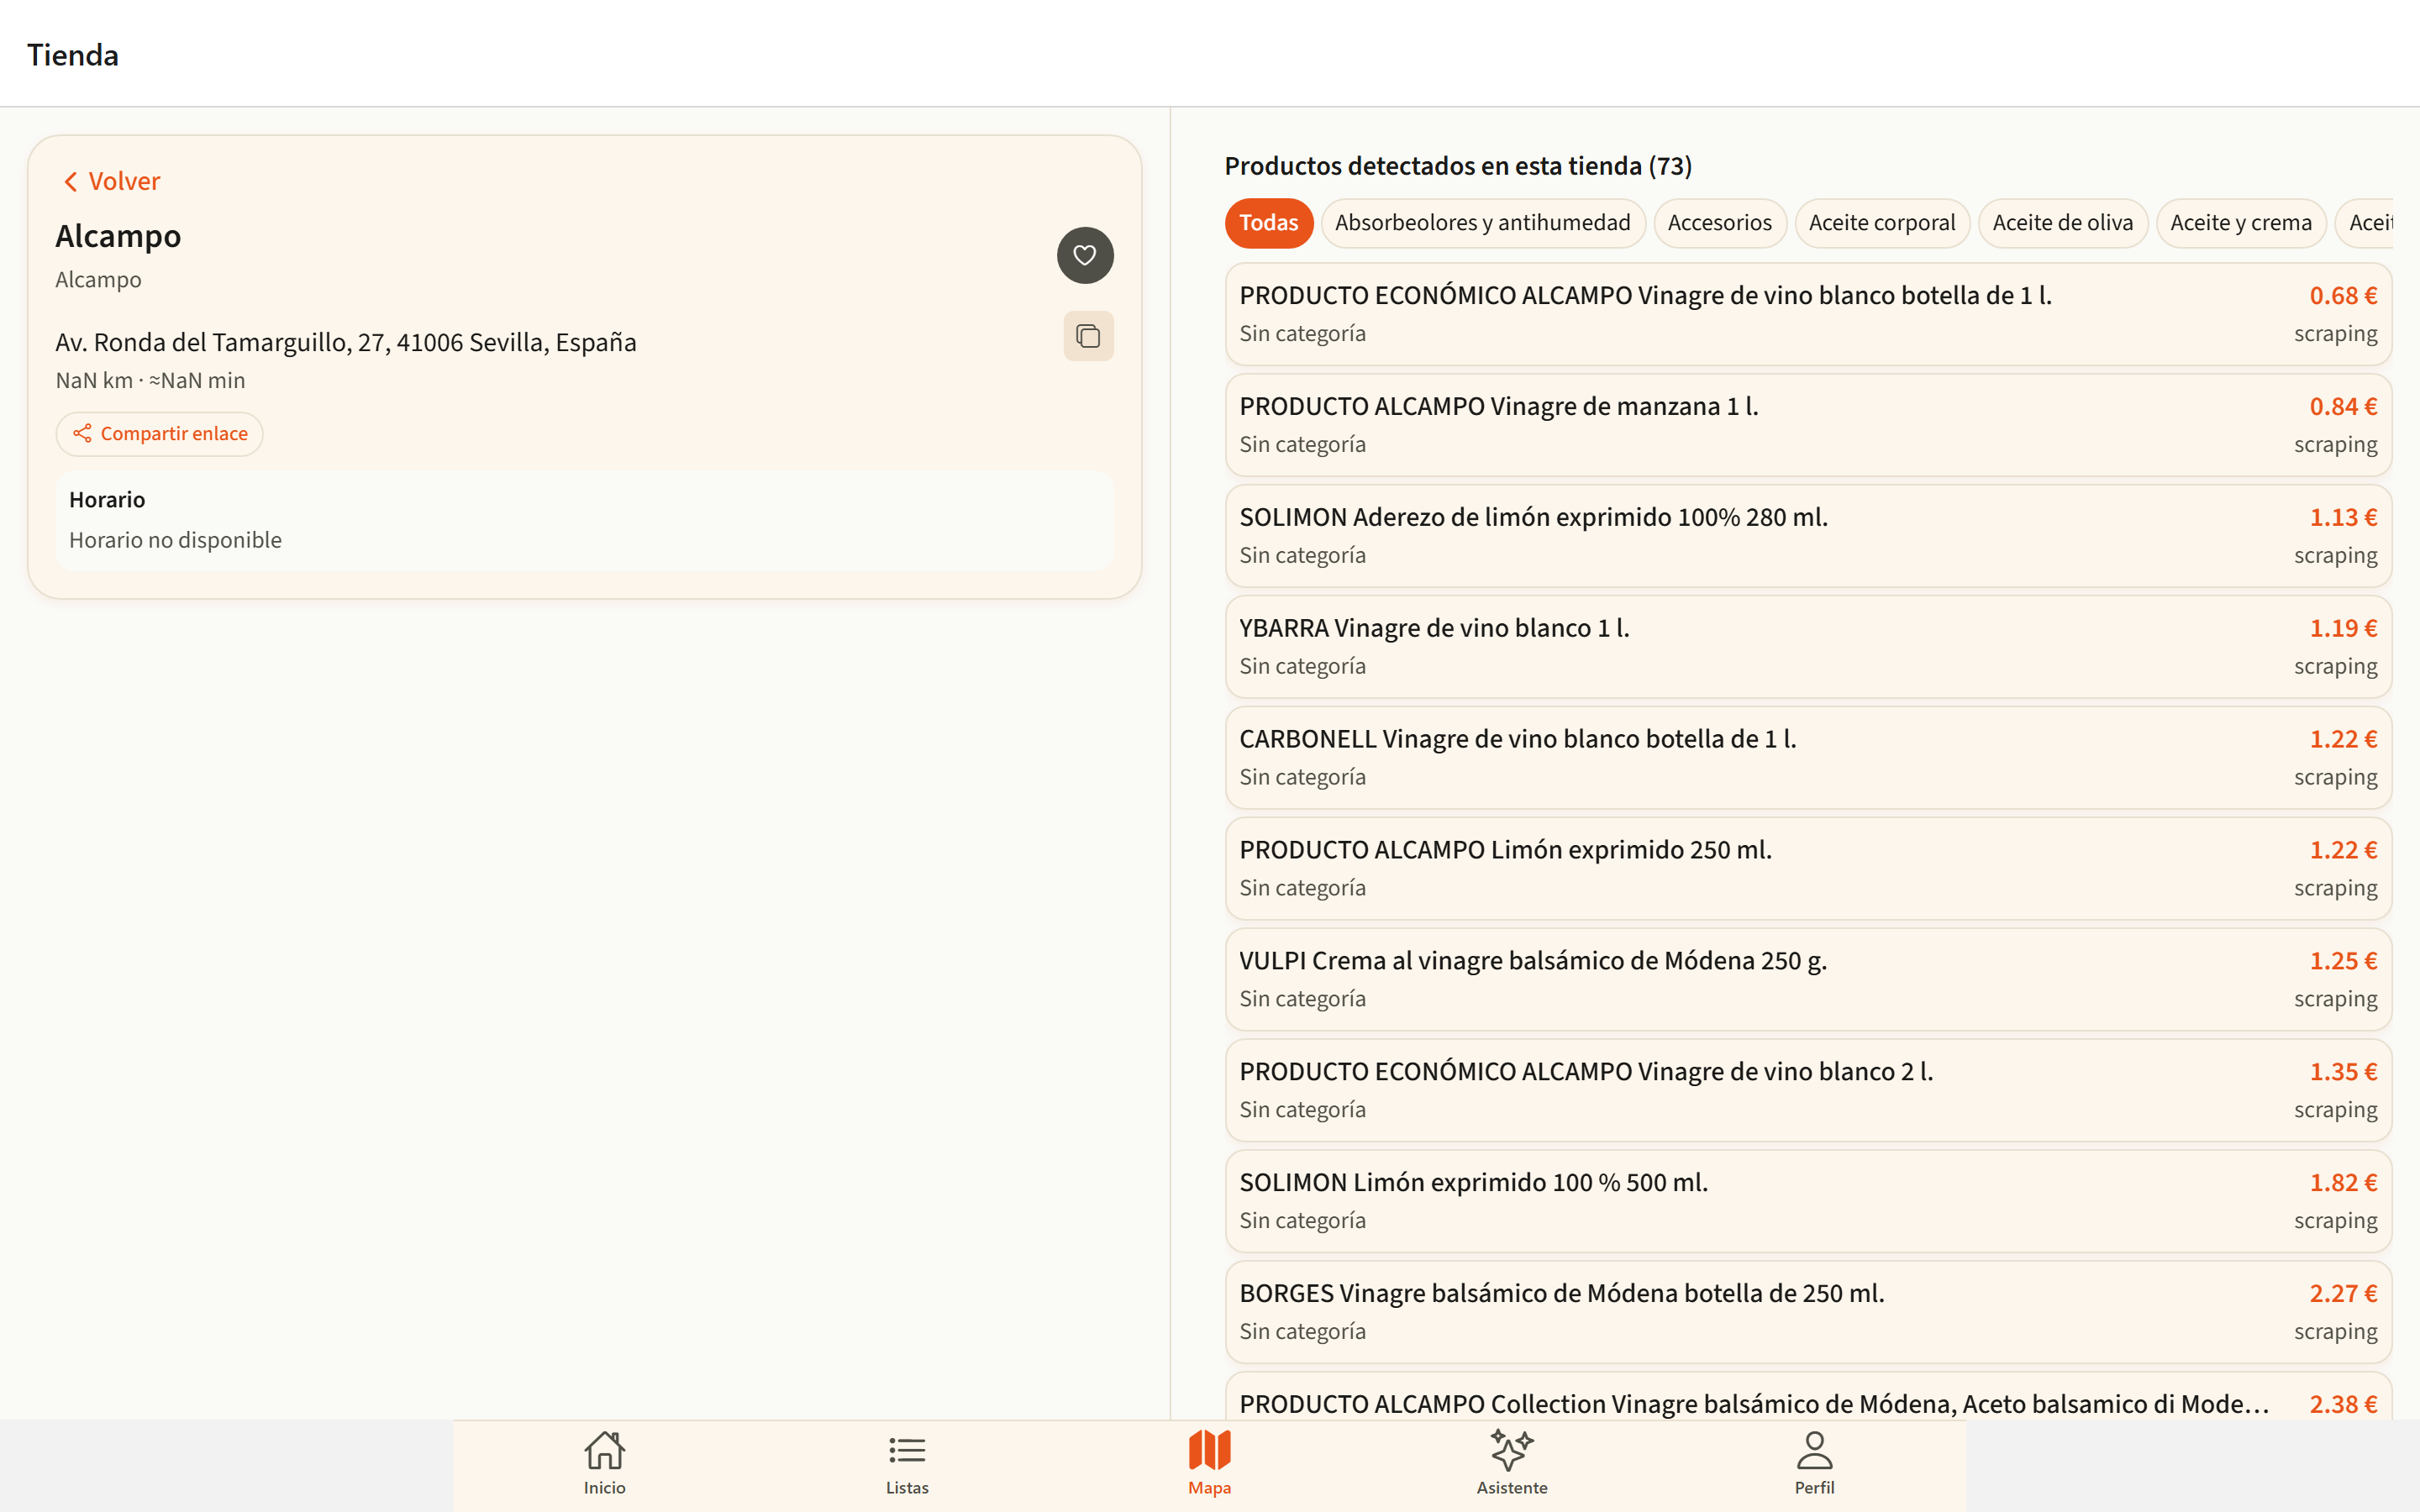
\includegraphics[width=0.46\textwidth]{diagramas/capturas/web-tienda-perfil.png}
\caption{Web --- Mapa con panel de tiendas anclado a la derecha (izquierda) y perfil de tienda a
dos columnas (derecha)}
\label{fig:cap-web-mapa-tienda}
\end{figure}

\clearpage

\begin{figure}[htbp]
\centering
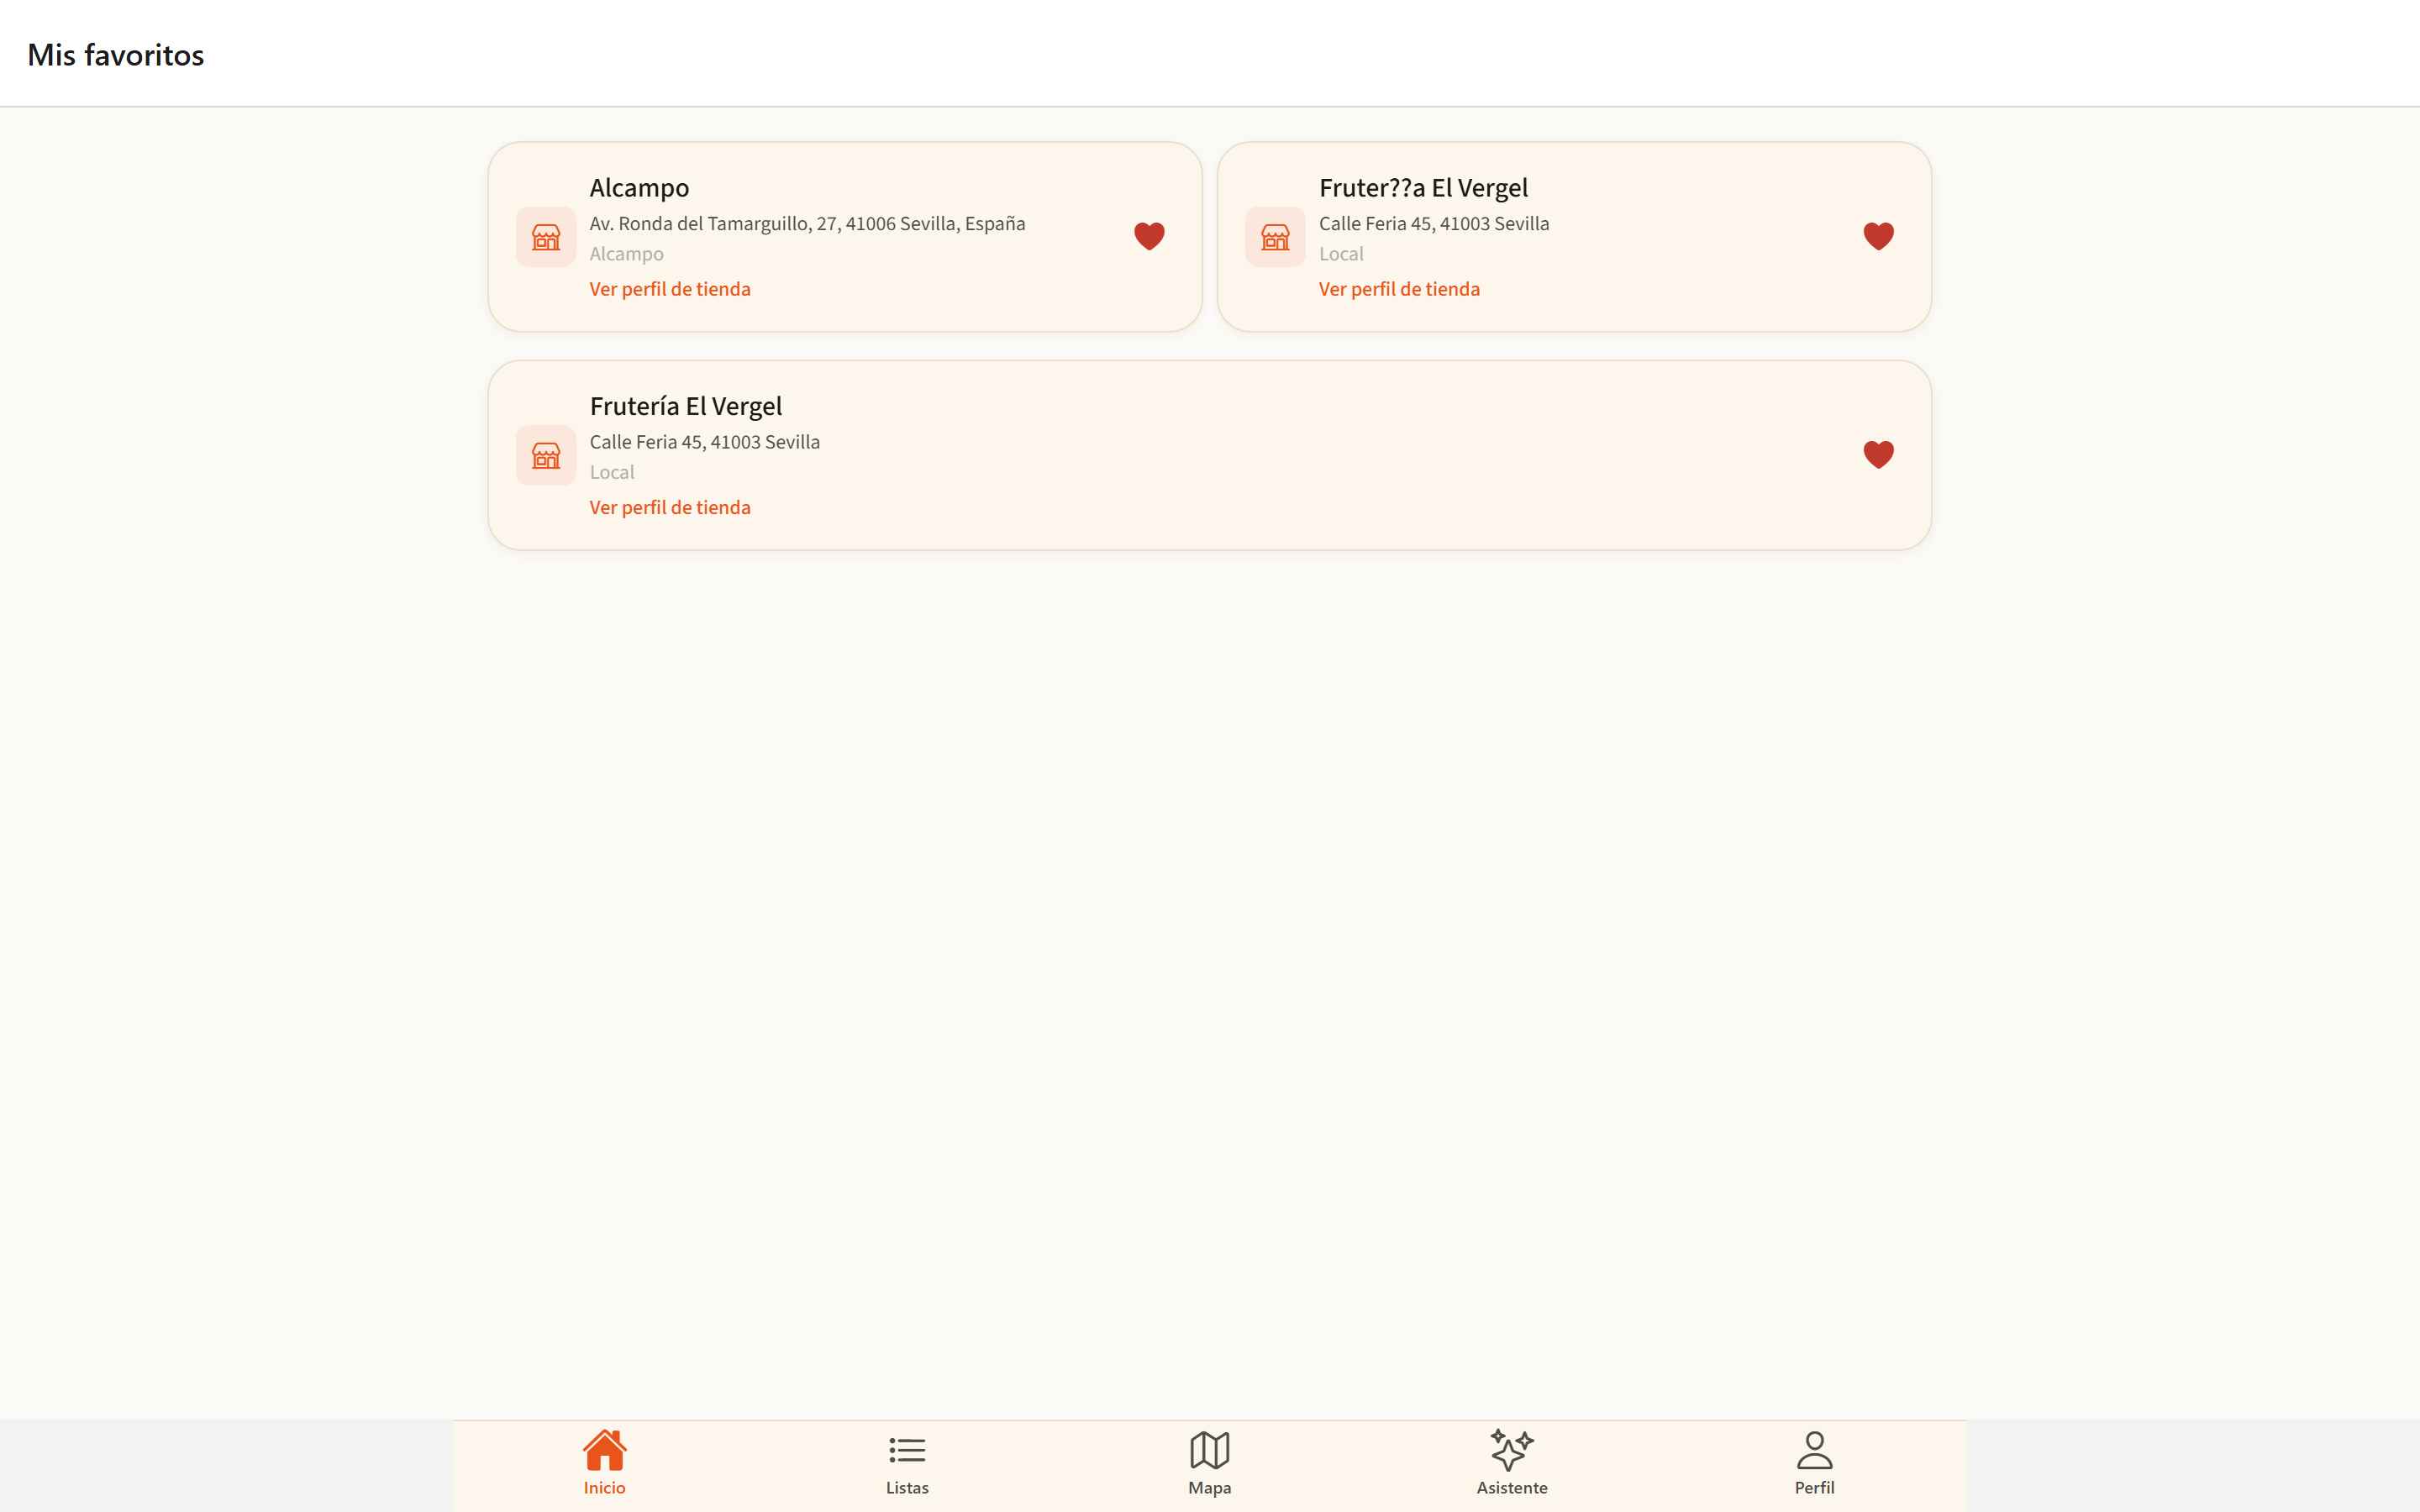
\includegraphics[width=0.46\textwidth]{diagramas/capturas/web-favoritas.png}
\hfill
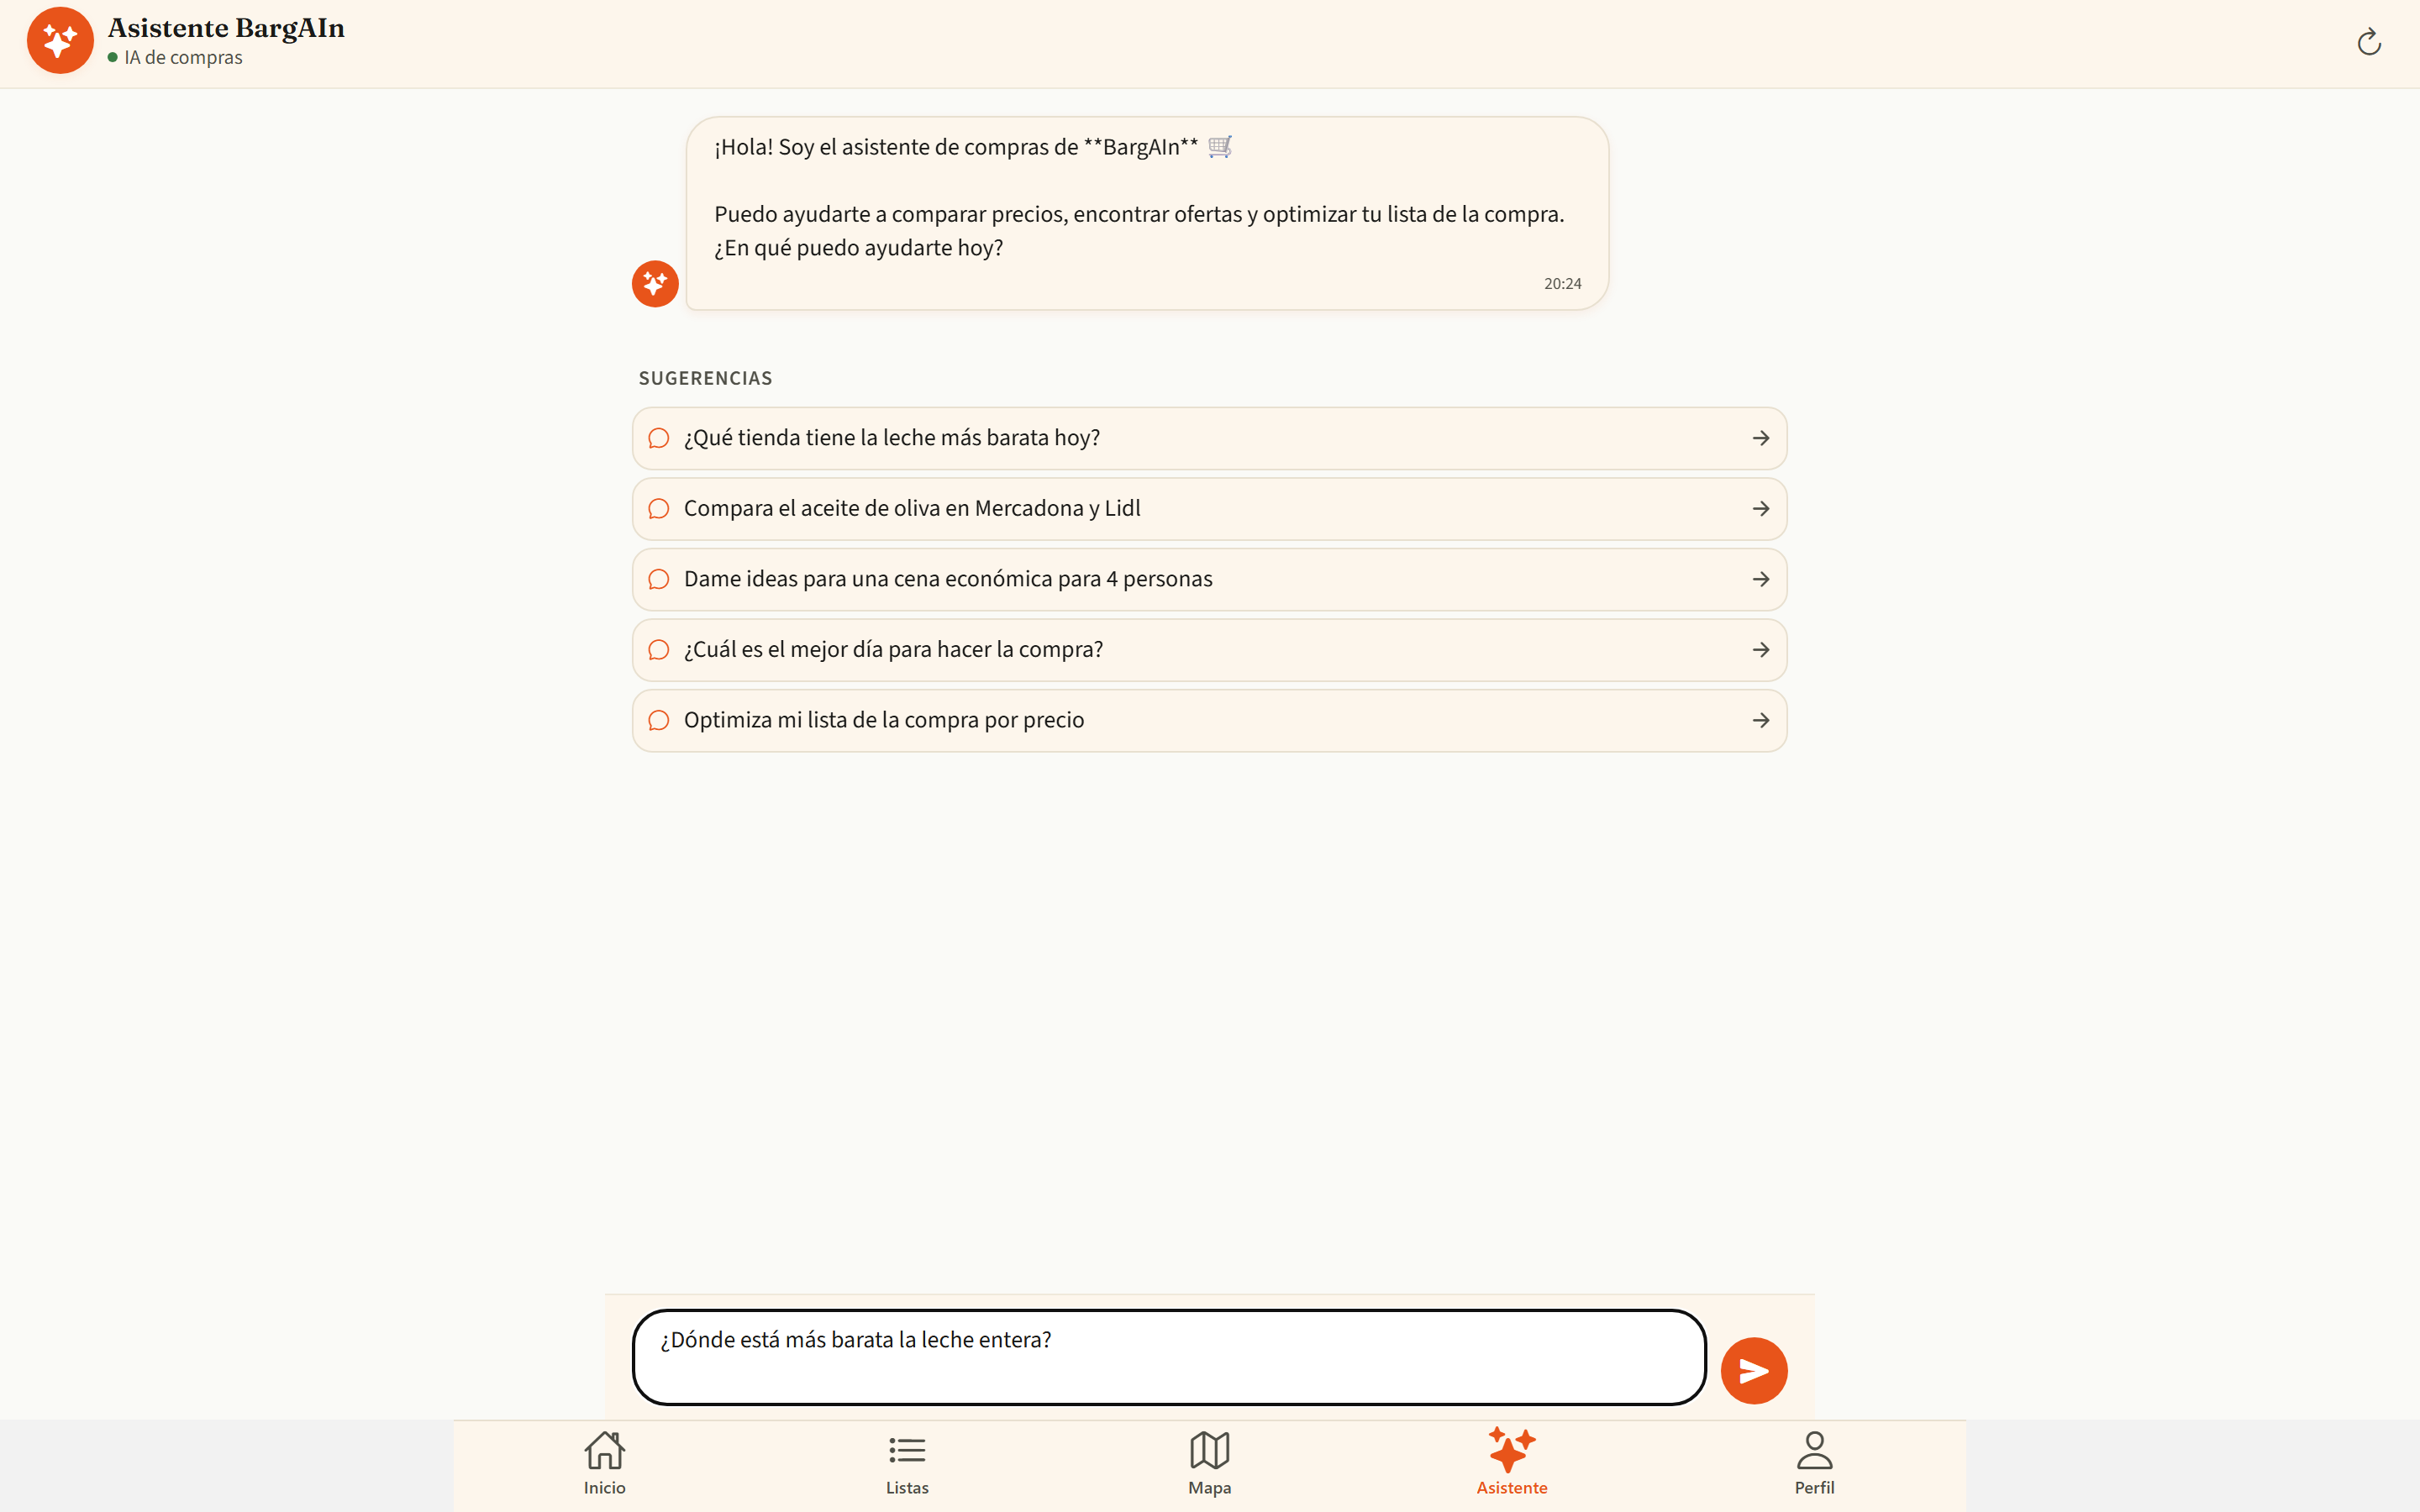
\includegraphics[width=0.46\textwidth]{diagramas/capturas/web-asistente.png}
\caption{Web --- Tiendas favoritas en rejilla (izquierda) y asistente centrado con copia por
mensaje (derecha)}
\label{fig:cap-web-favoritas-asistente}
\end{figure}

\begin{figure}[htbp]
\centering
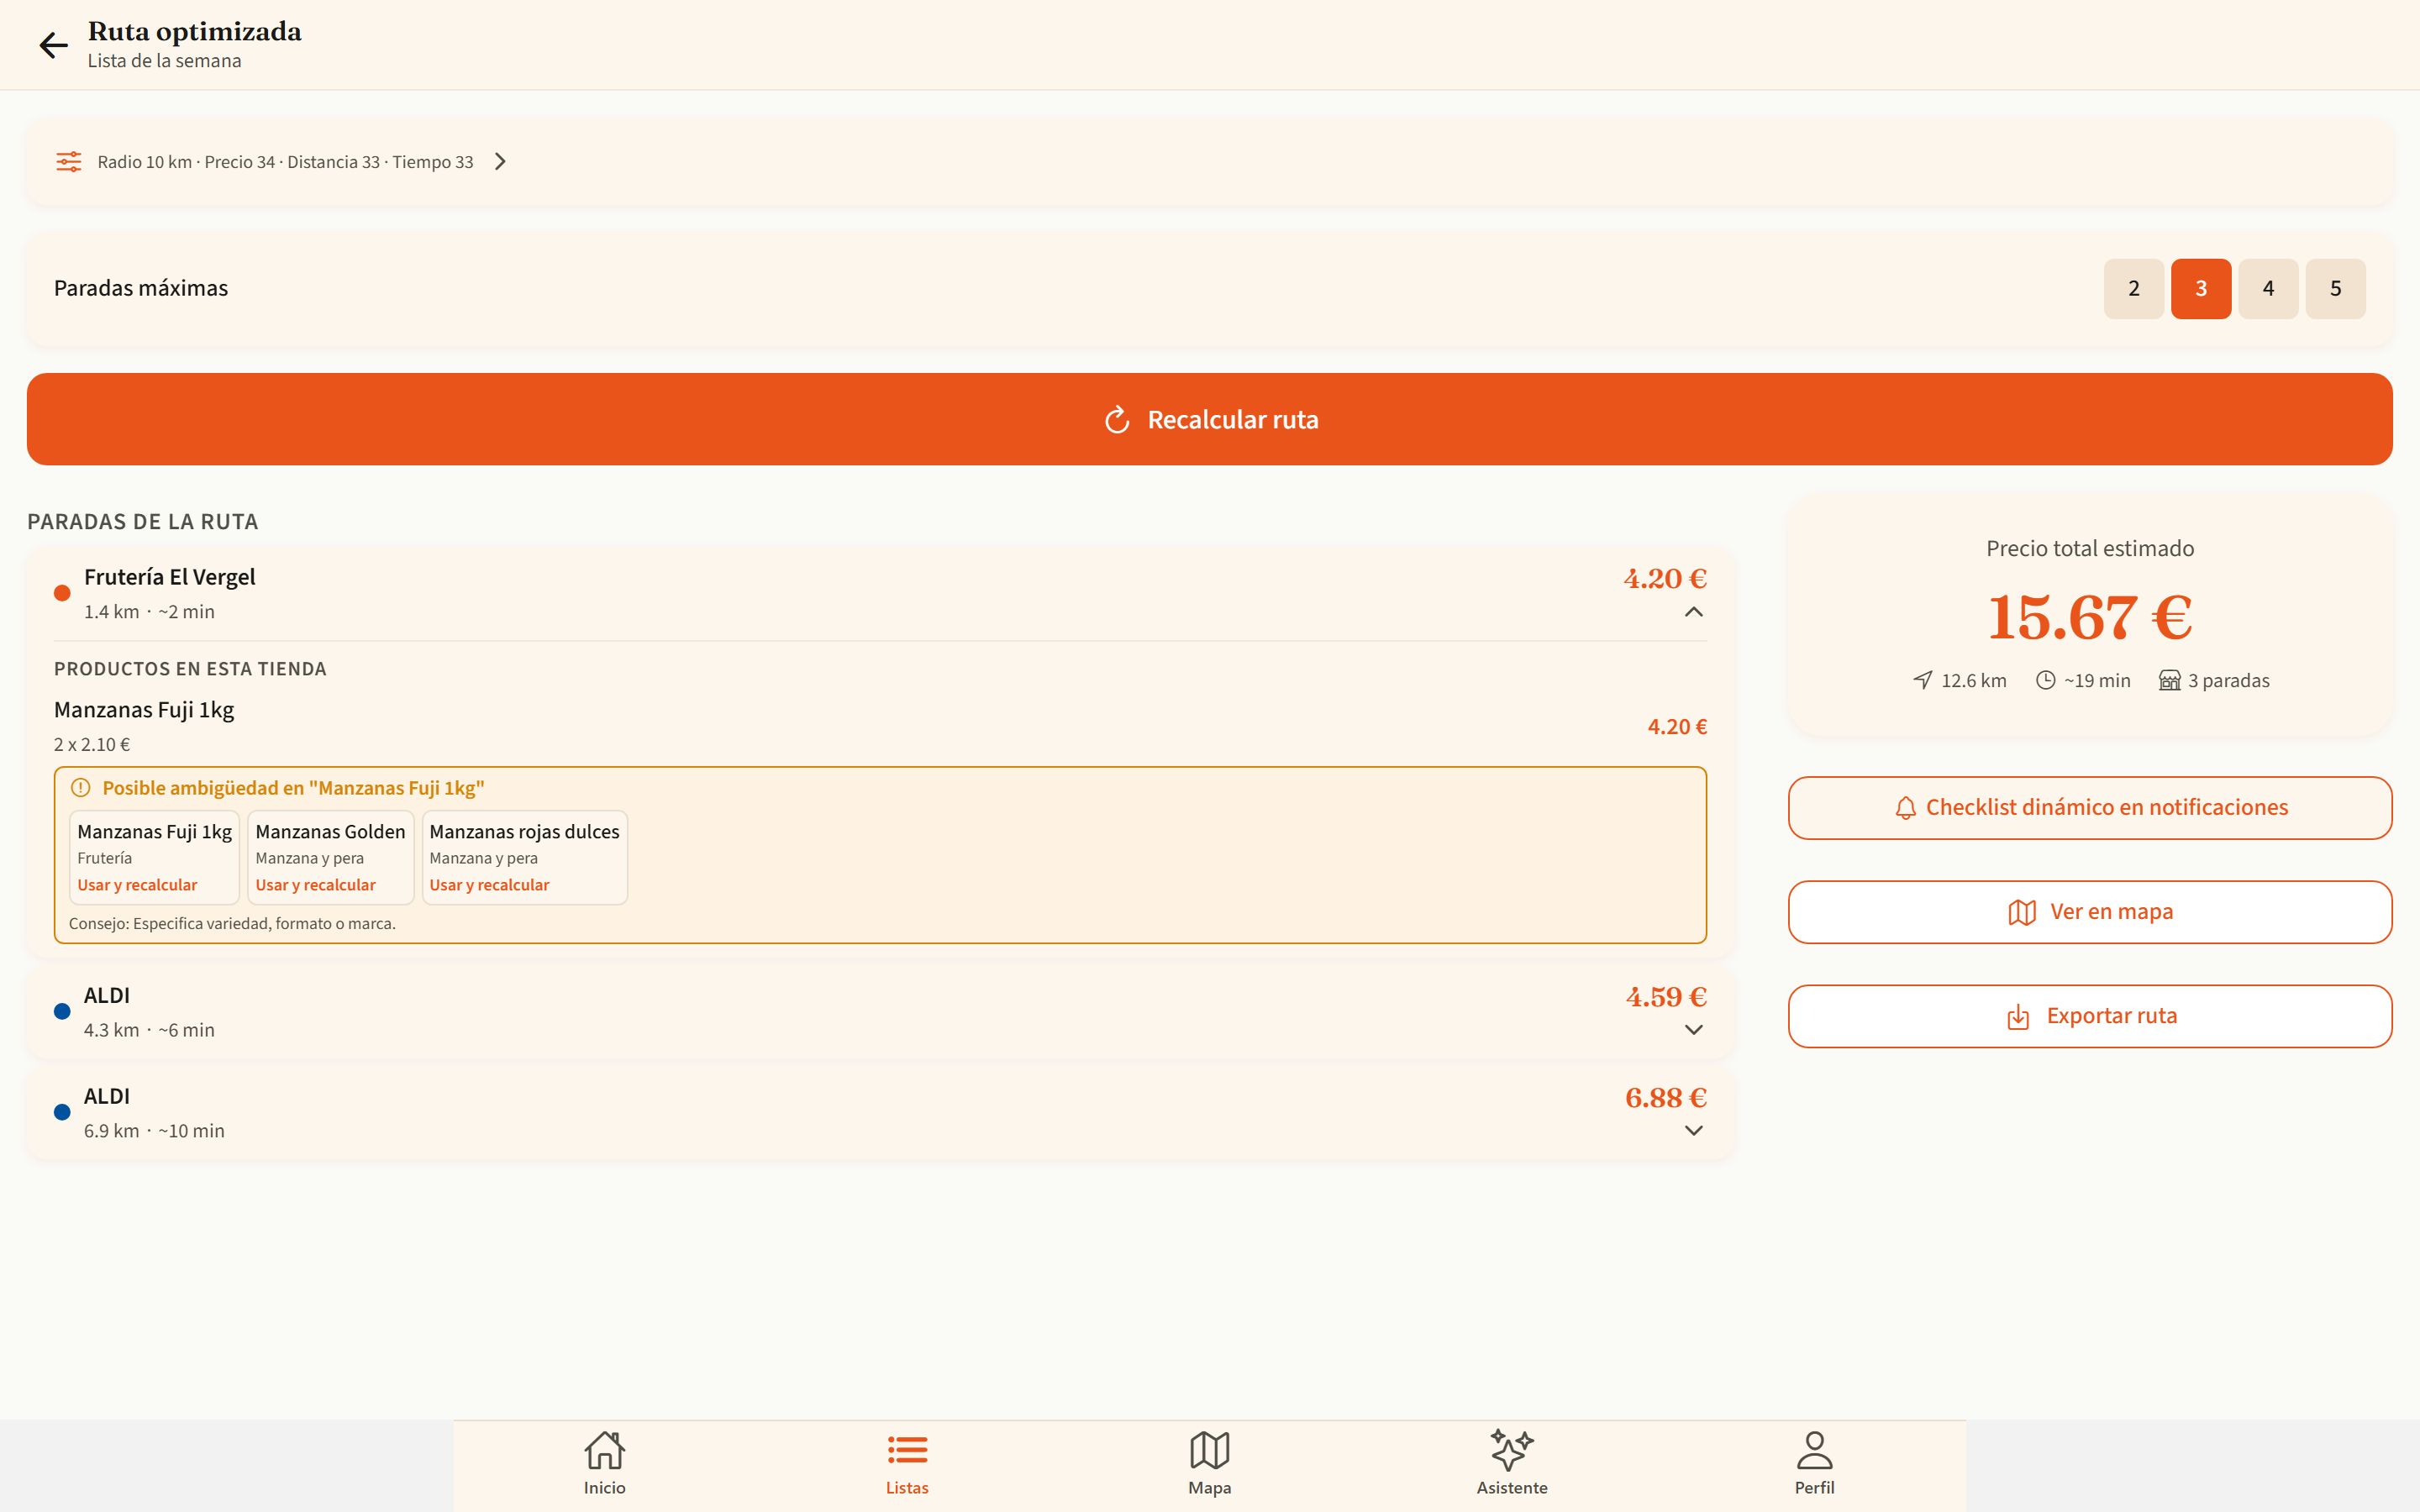
\includegraphics[width=0.46\textwidth]{diagramas/capturas/web-ruta.png}
\hfill
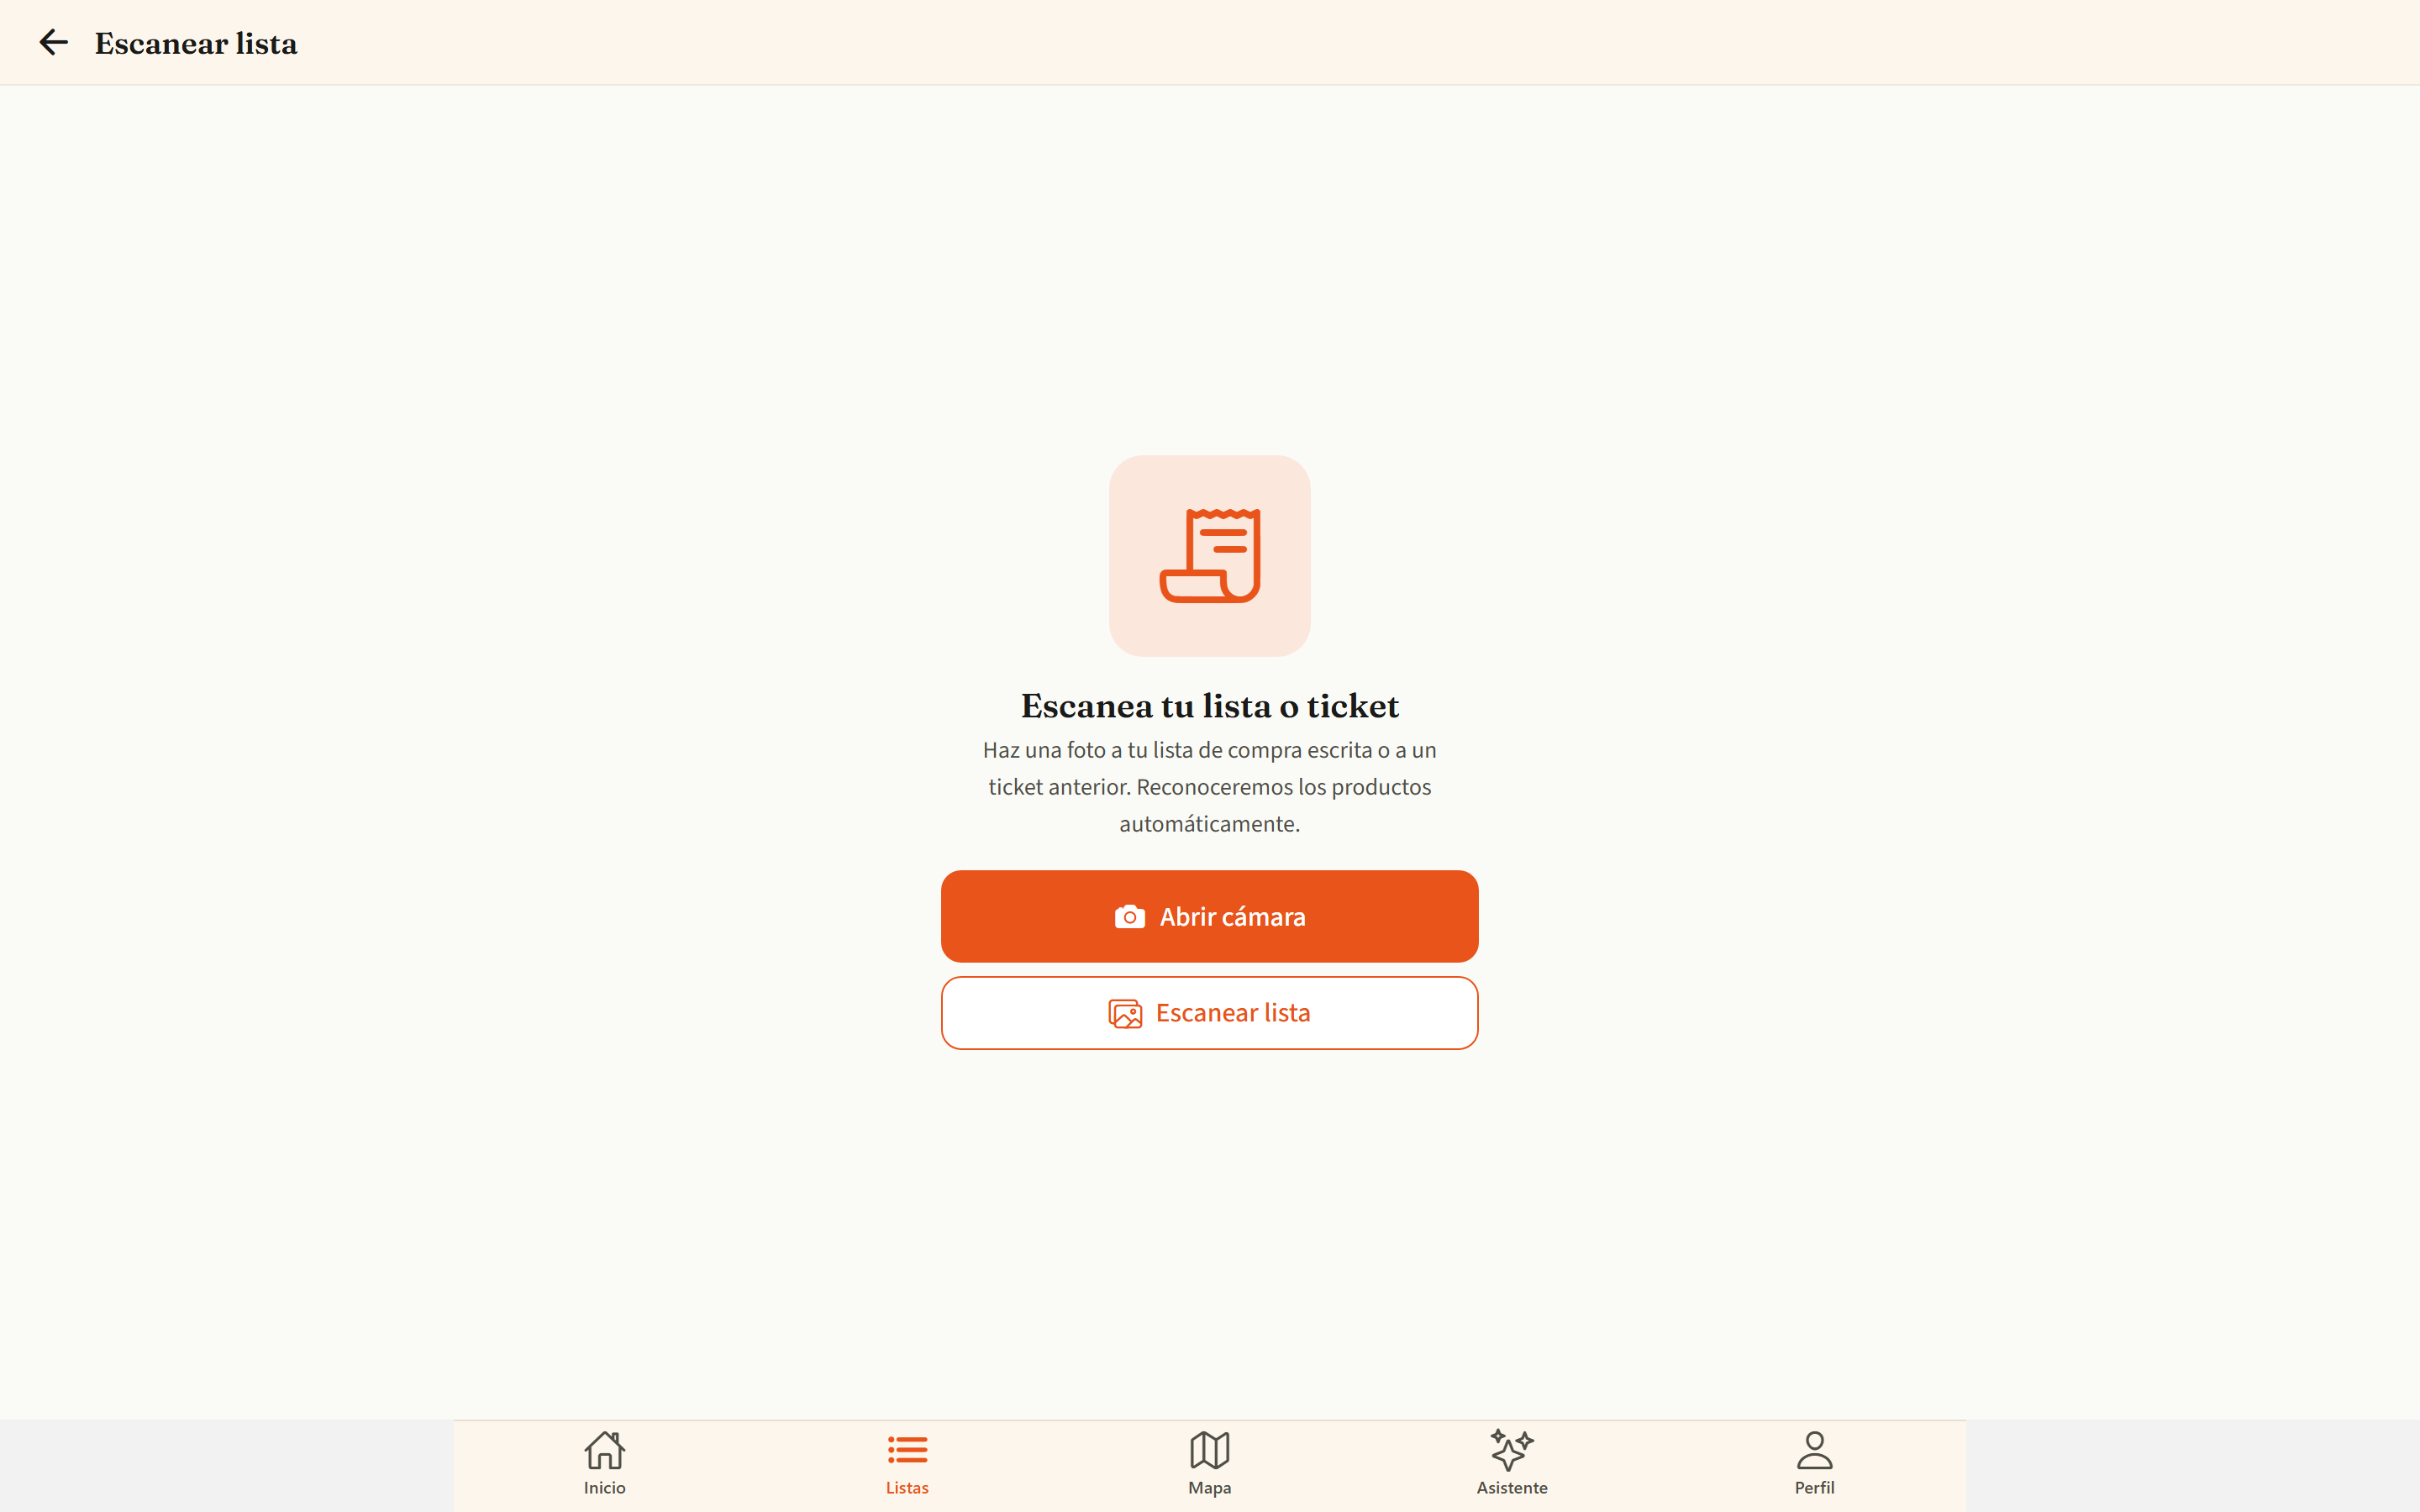
\includegraphics[width=0.46\textwidth]{diagramas/capturas/web-ocr.png}
\caption{Web --- Ruta optimizada con exportaci\'on (izquierda) y m\'odulo OCR centrado (derecha)}
\label{fig:cap-web-ruta-ocr}
\end{figure}

\begin{figure}[htbp]
\centering
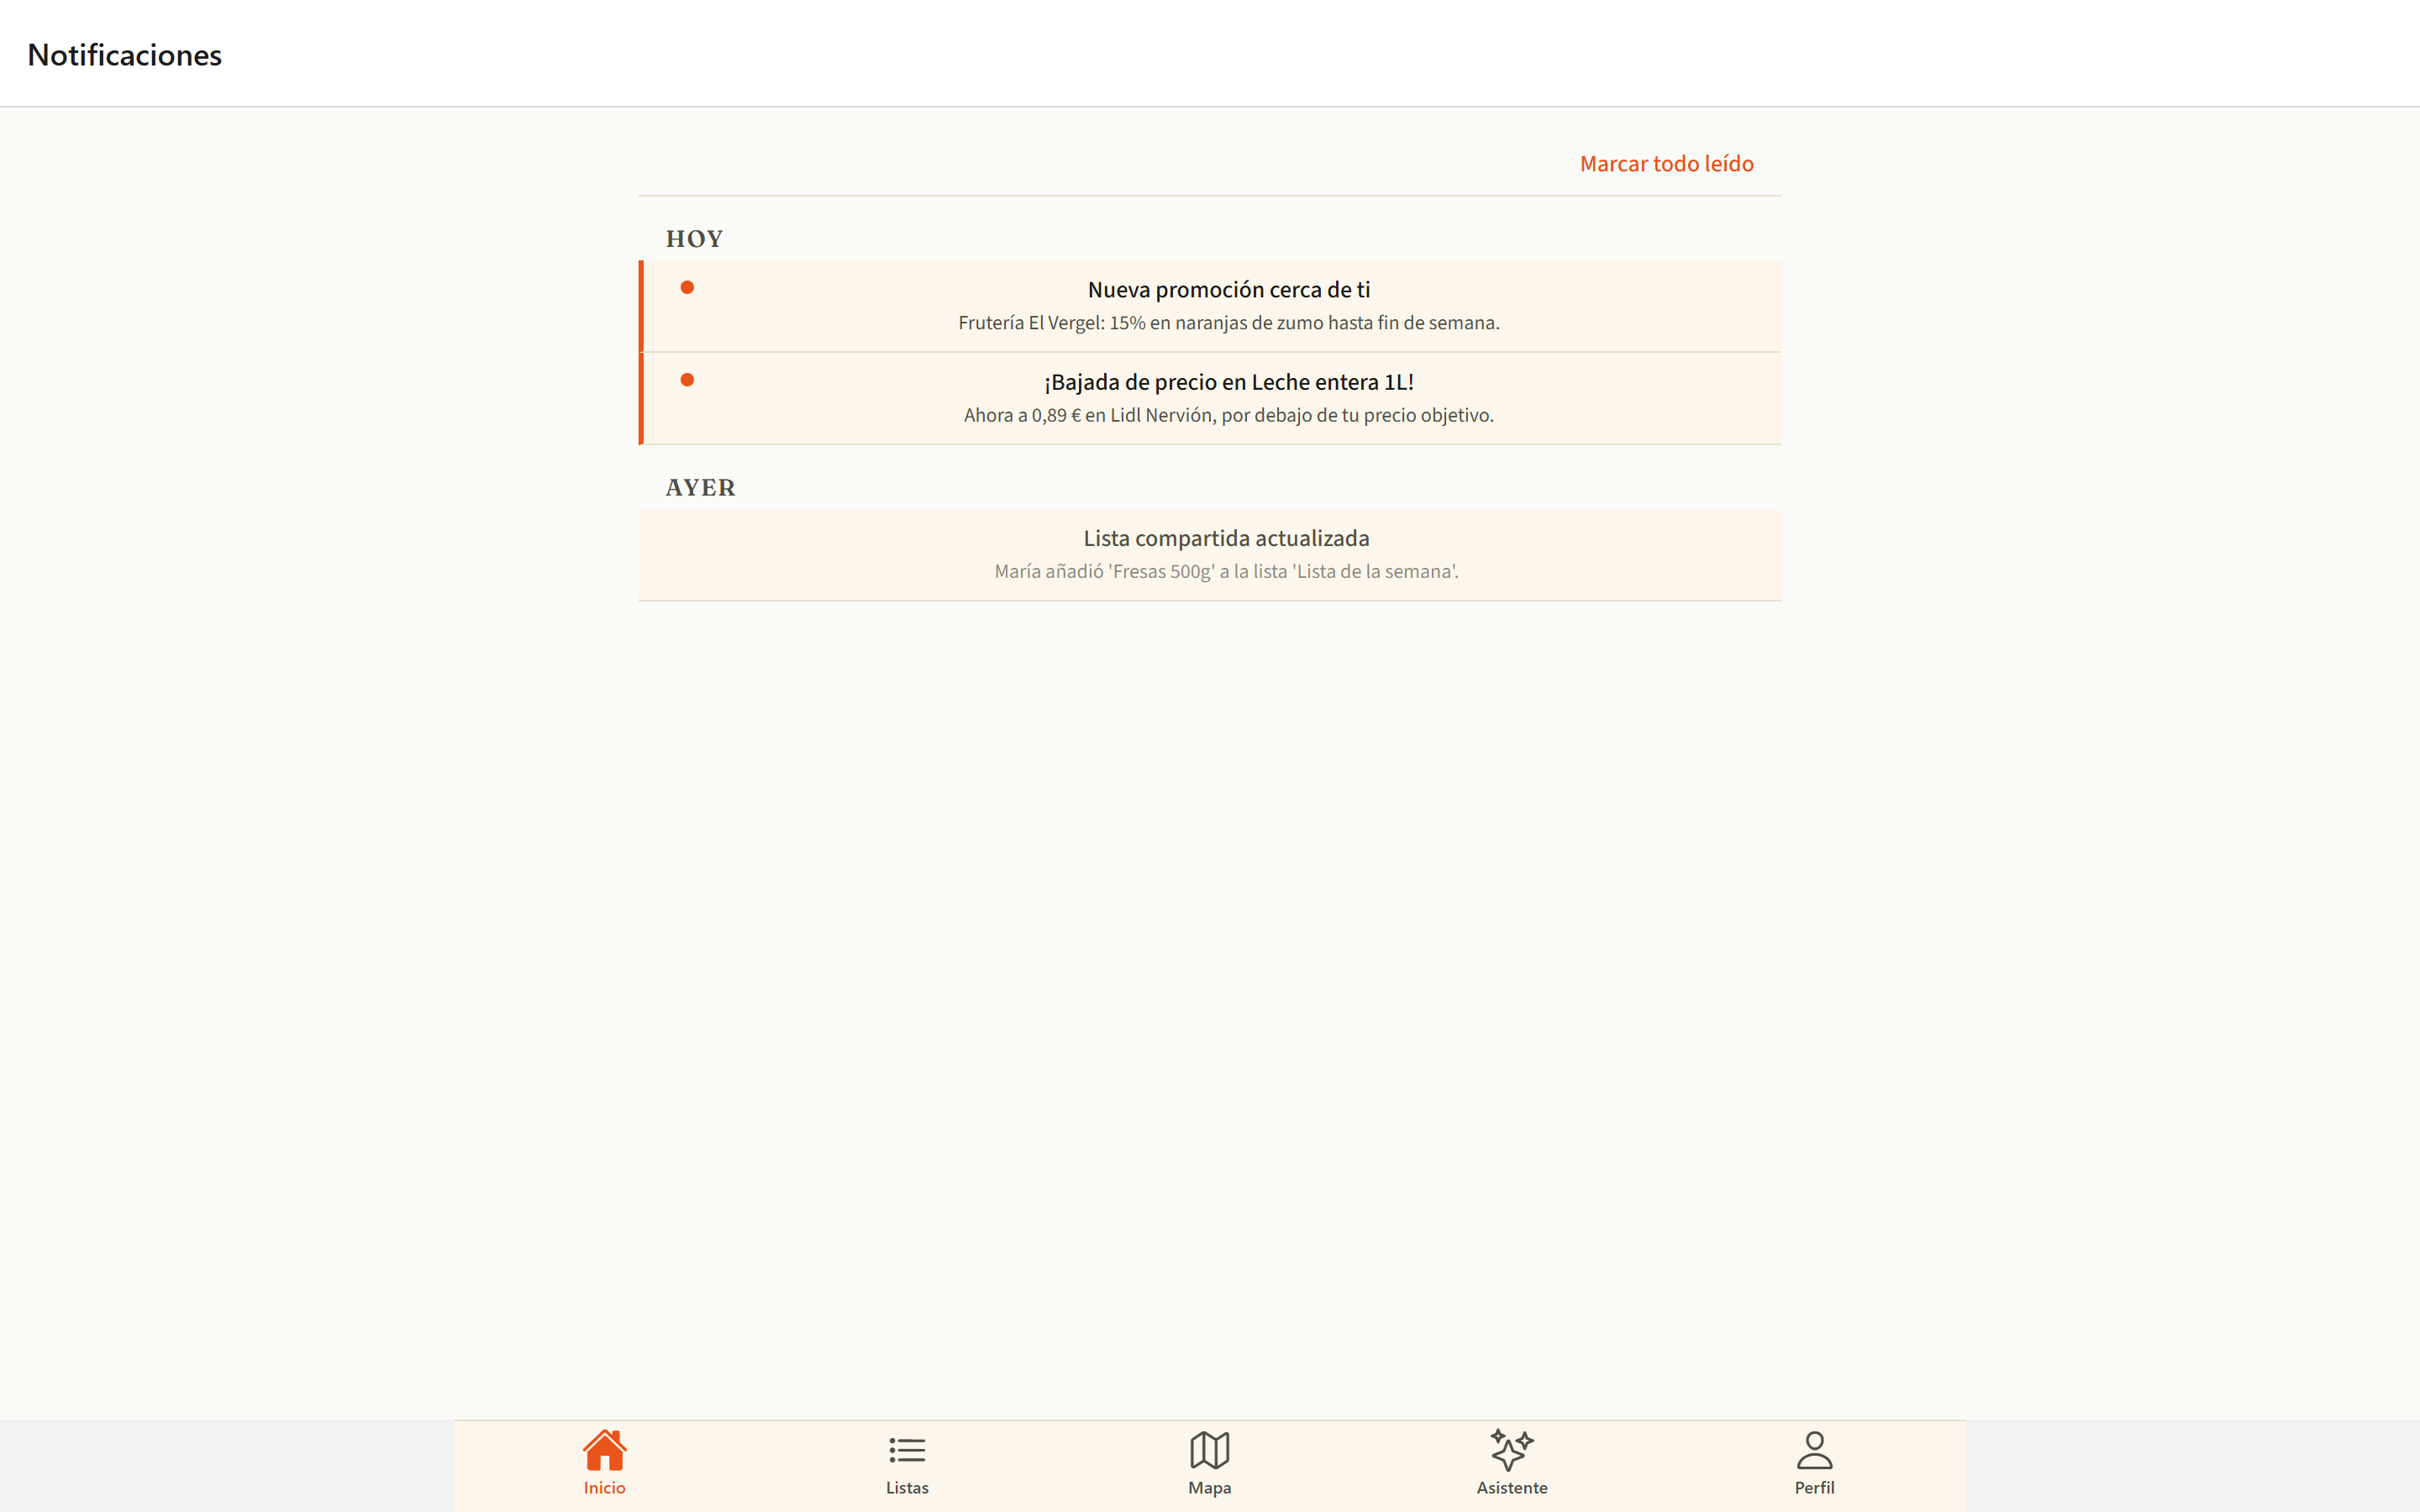
\includegraphics[width=0.46\textwidth]{diagramas/capturas/web-notificaciones.png}
\hfill
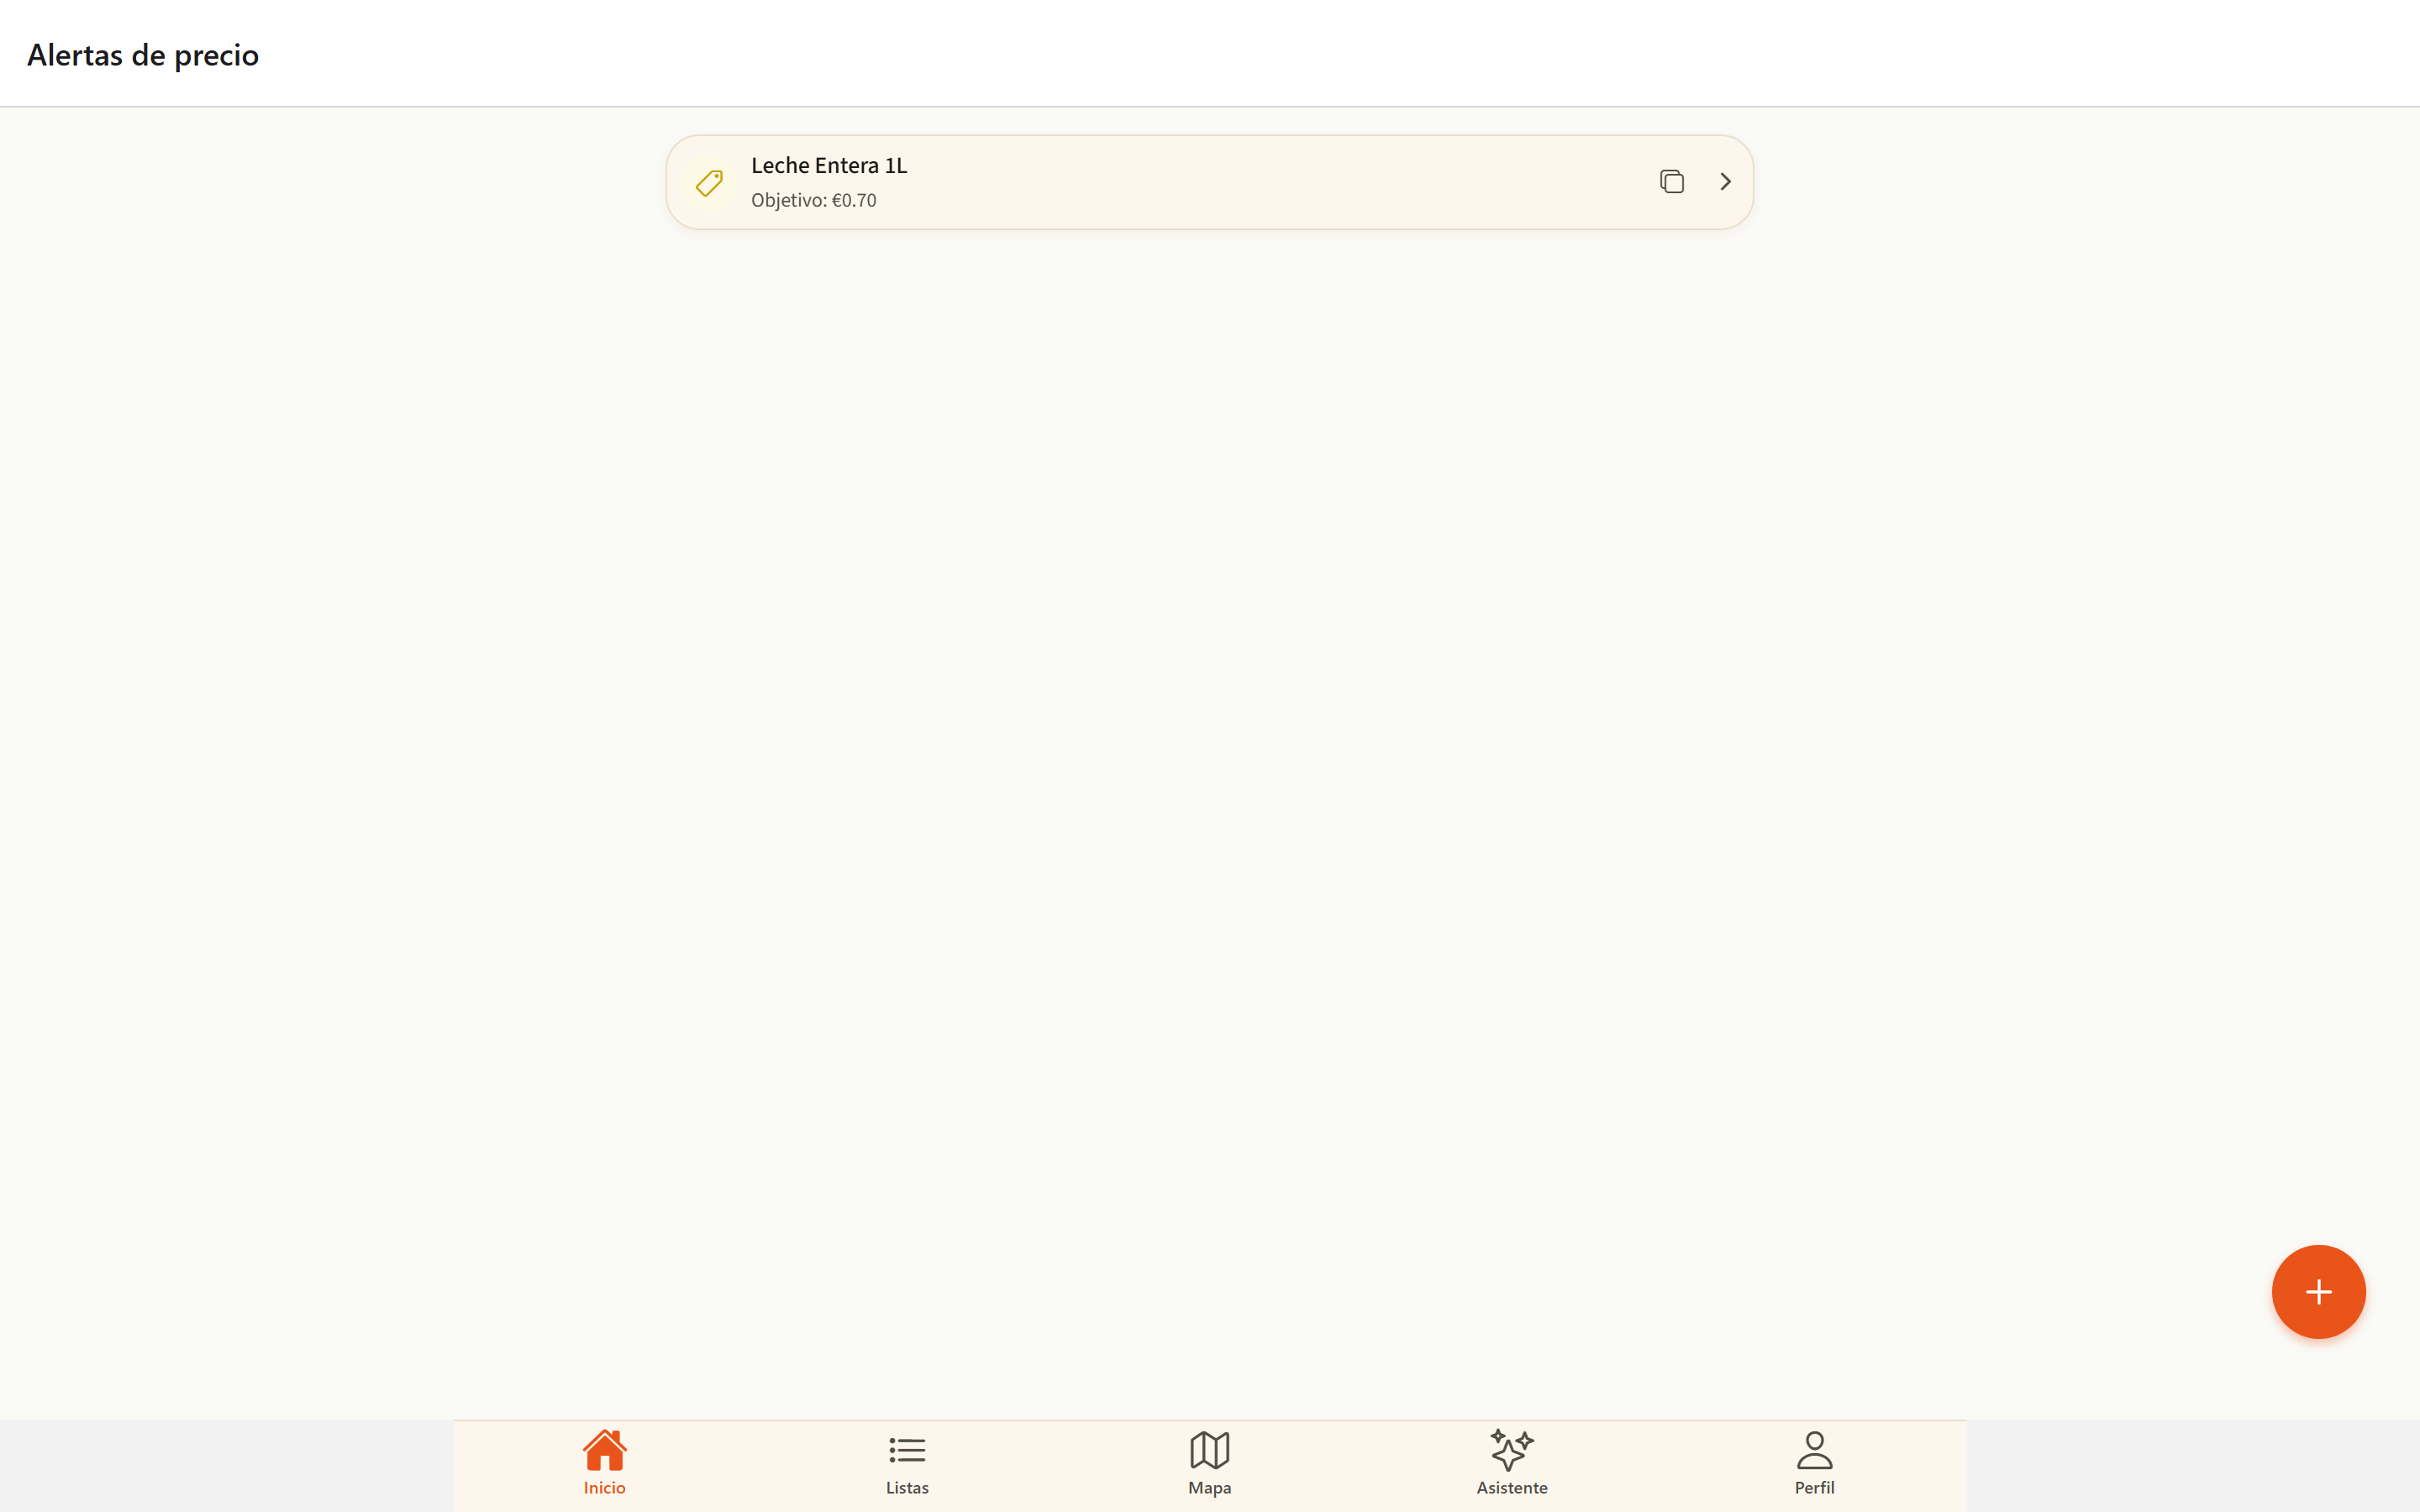
\includegraphics[width=0.46\textwidth]{diagramas/capturas/web-alertas.png}
\caption{Web --- Bandeja de notificaciones (izquierda) y alertas de precio (derecha) centradas}
\label{fig:cap-web-notif-alertas}
\end{figure}

\clearpage

\subsection{Portal web para PYMEs}\label{subsec:galeria-pyme}

\begin{figure}[htbp]
\centering
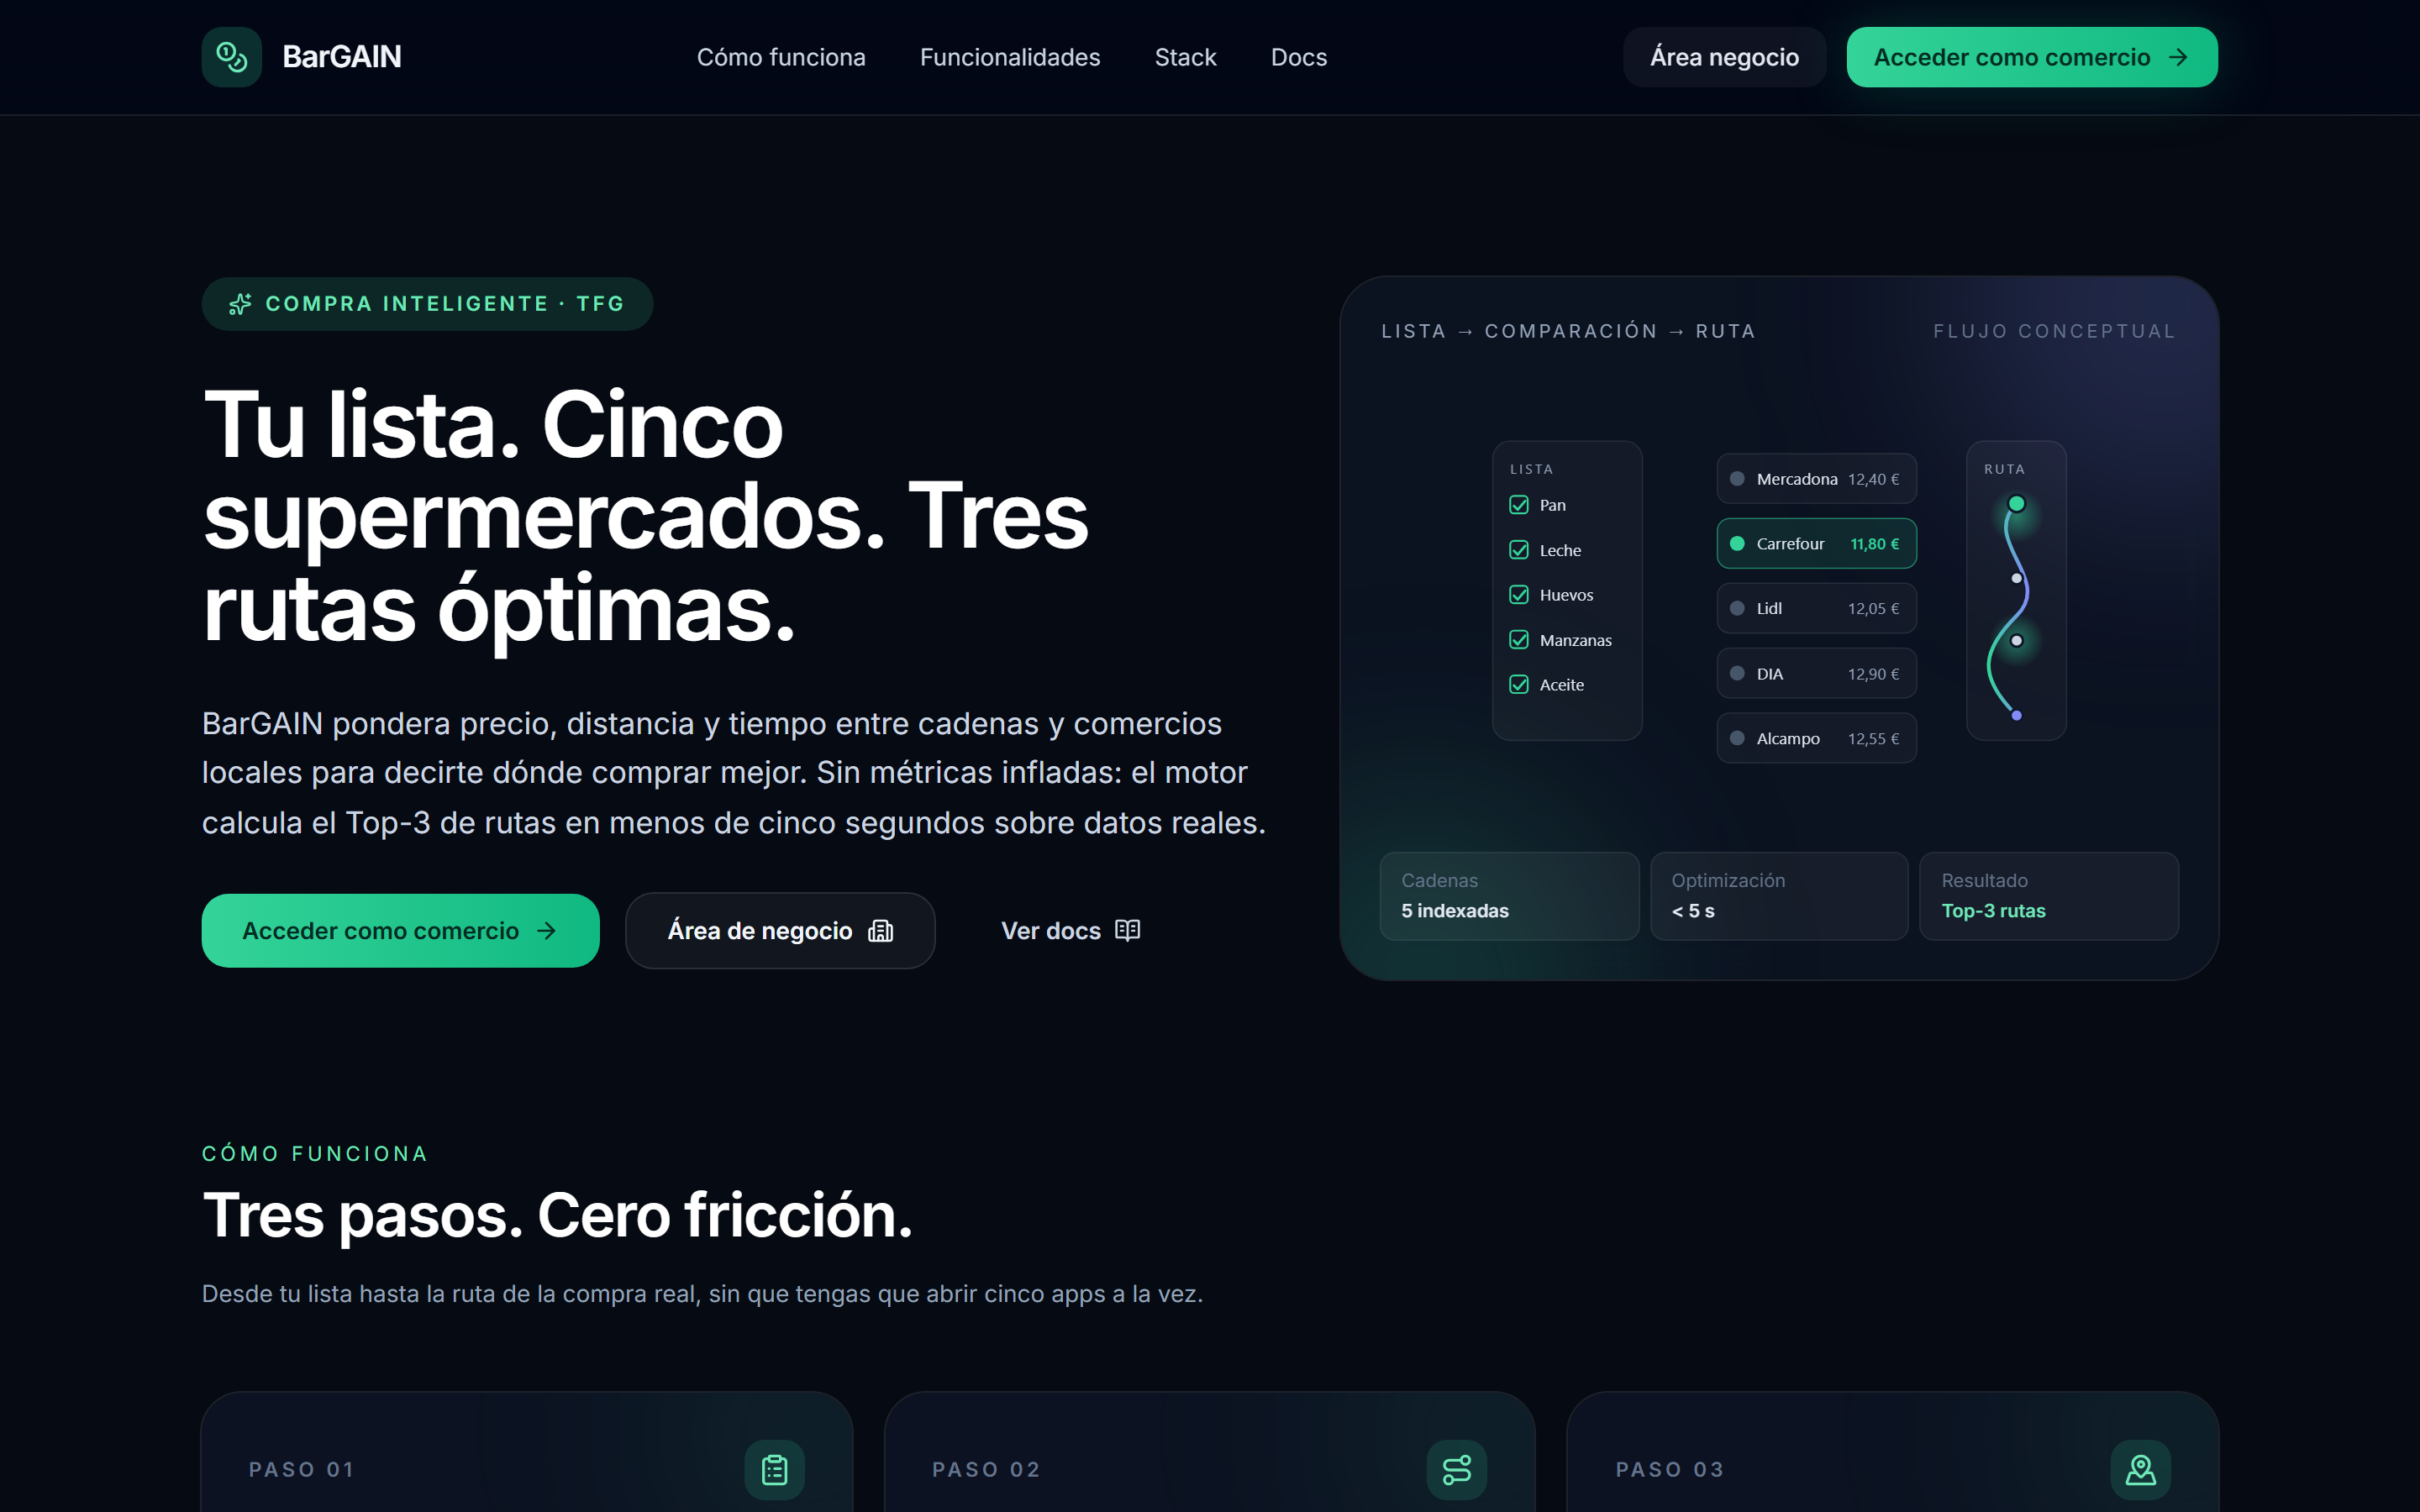
\includegraphics[width=0.85\textwidth]{diagramas/capturas/pyme-landing.png}
\caption{Portal PYME --- P\'agina de aterrizaje (\emph{landing})}
\label{fig:cap-pyme-landing}
\end{figure}

\begin{figure}[htbp]
\centering
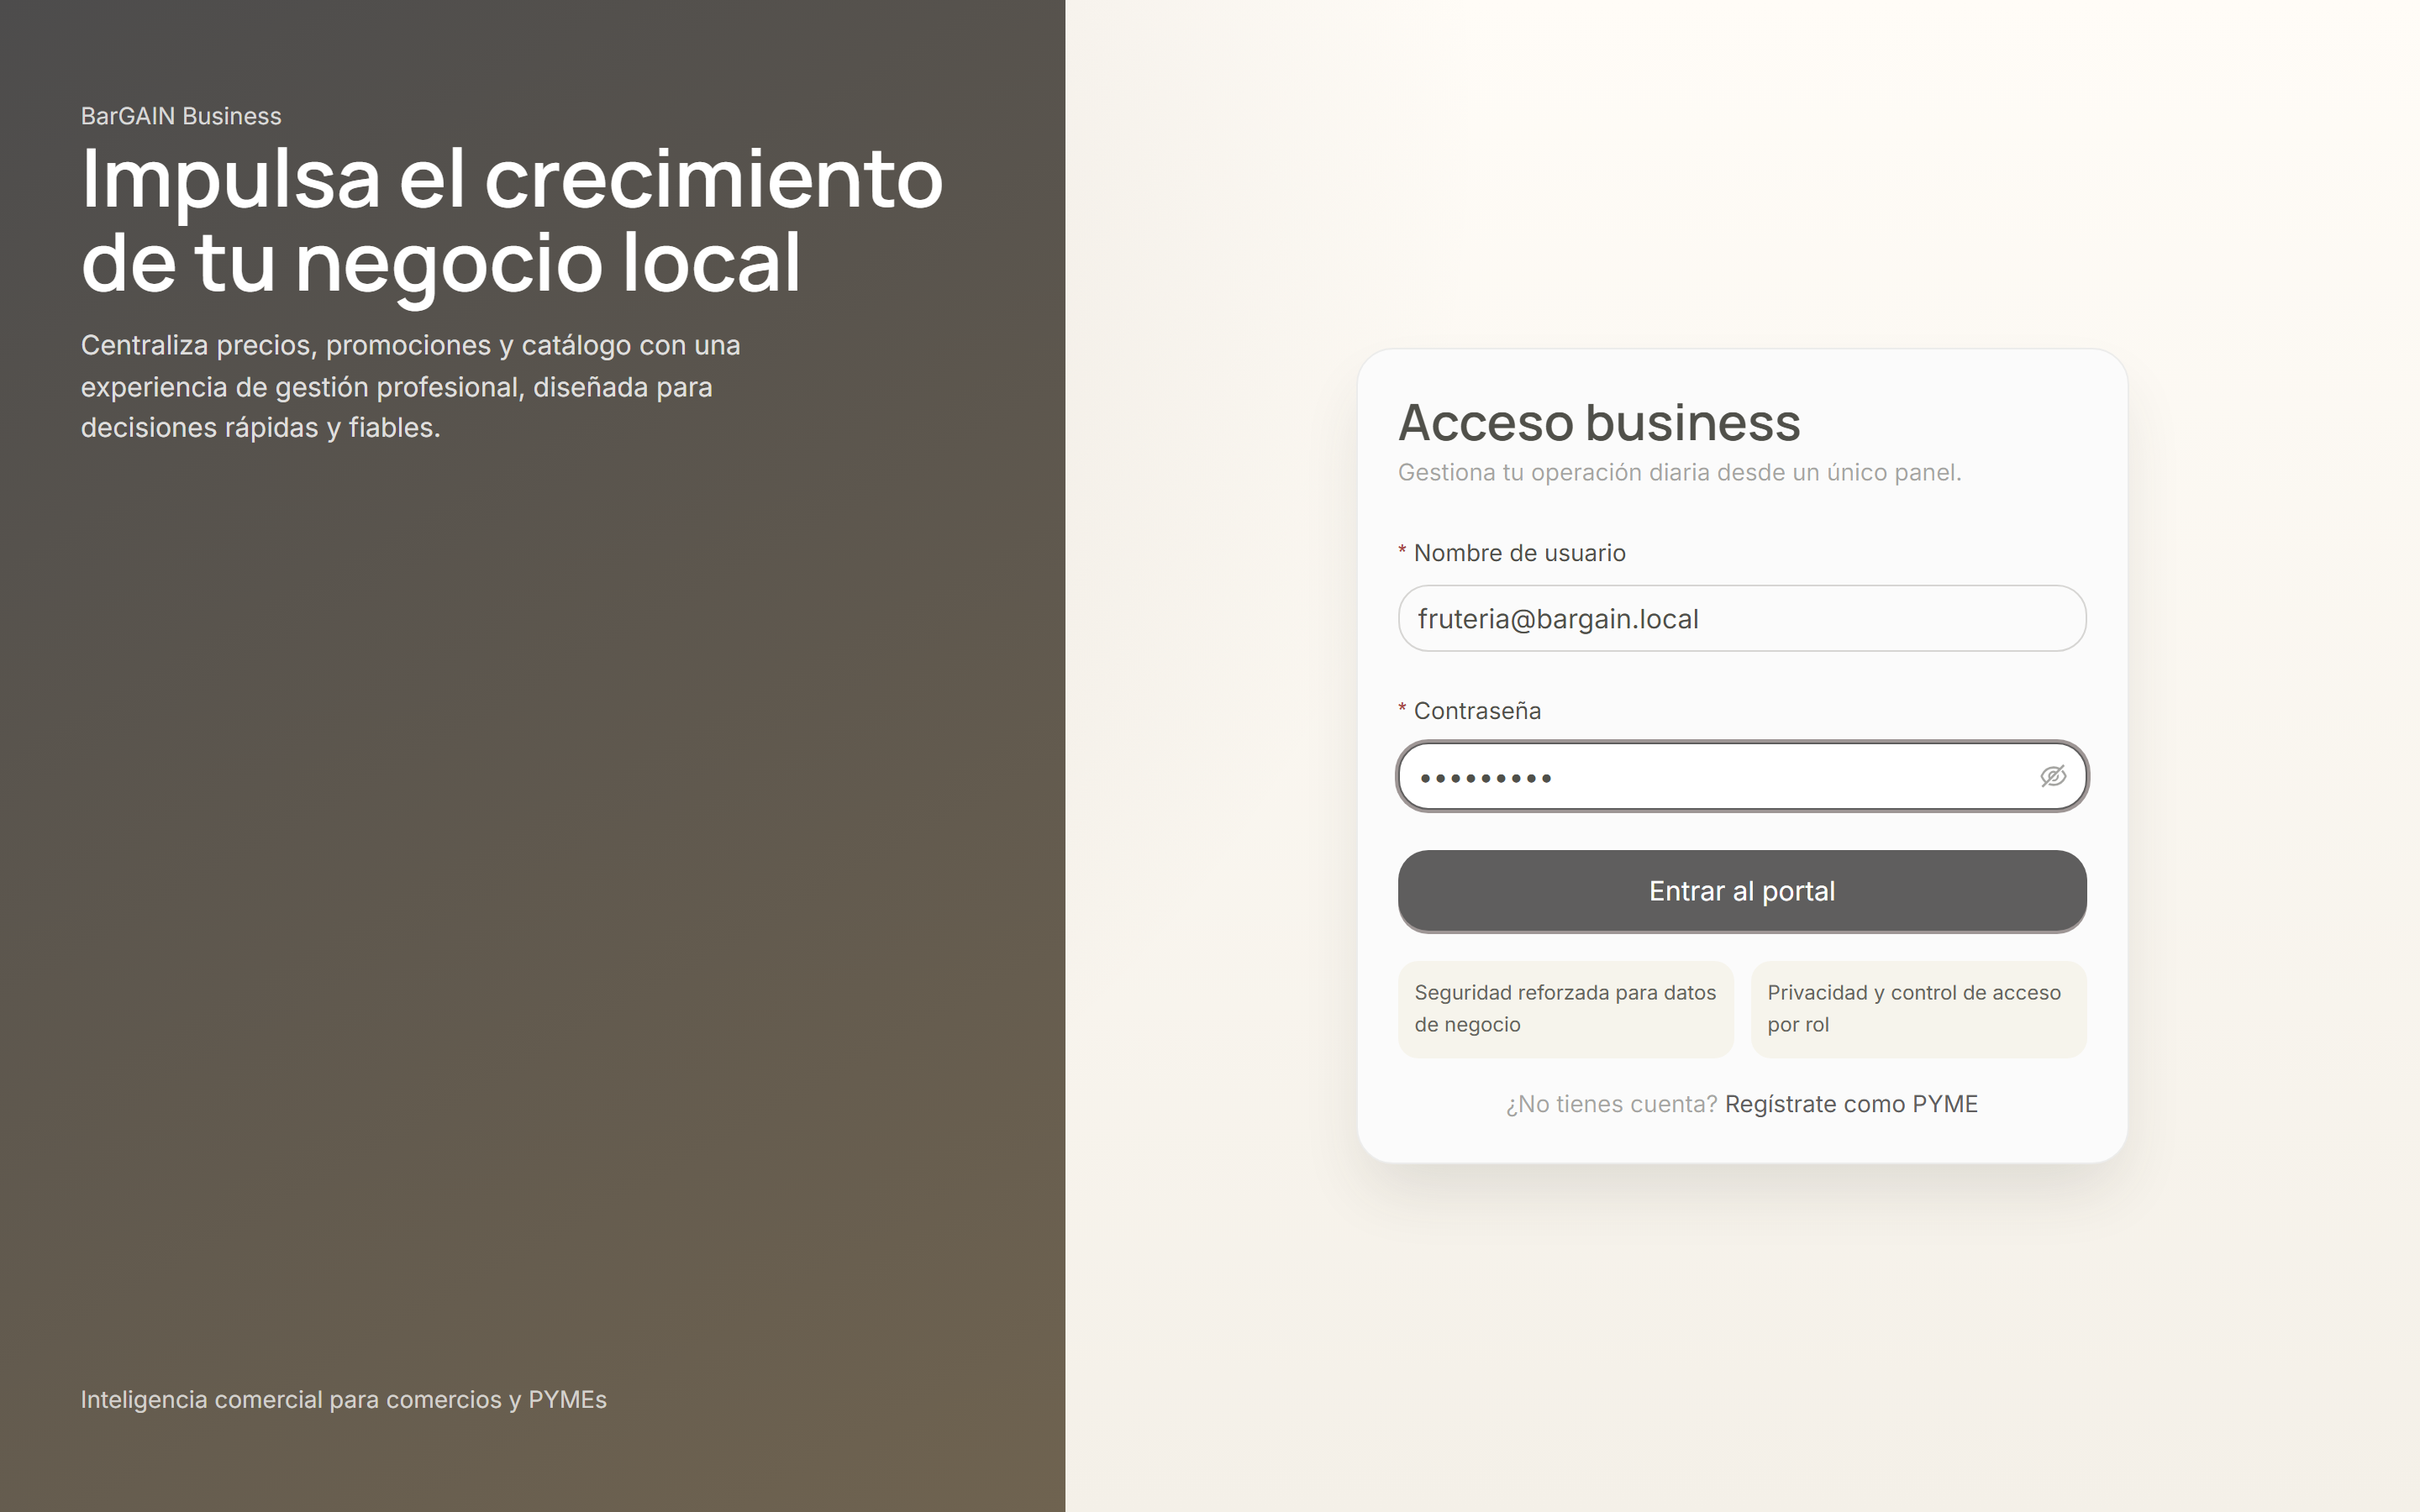
\includegraphics[width=0.46\textwidth]{diagramas/capturas/pyme-login.png}
\hfill
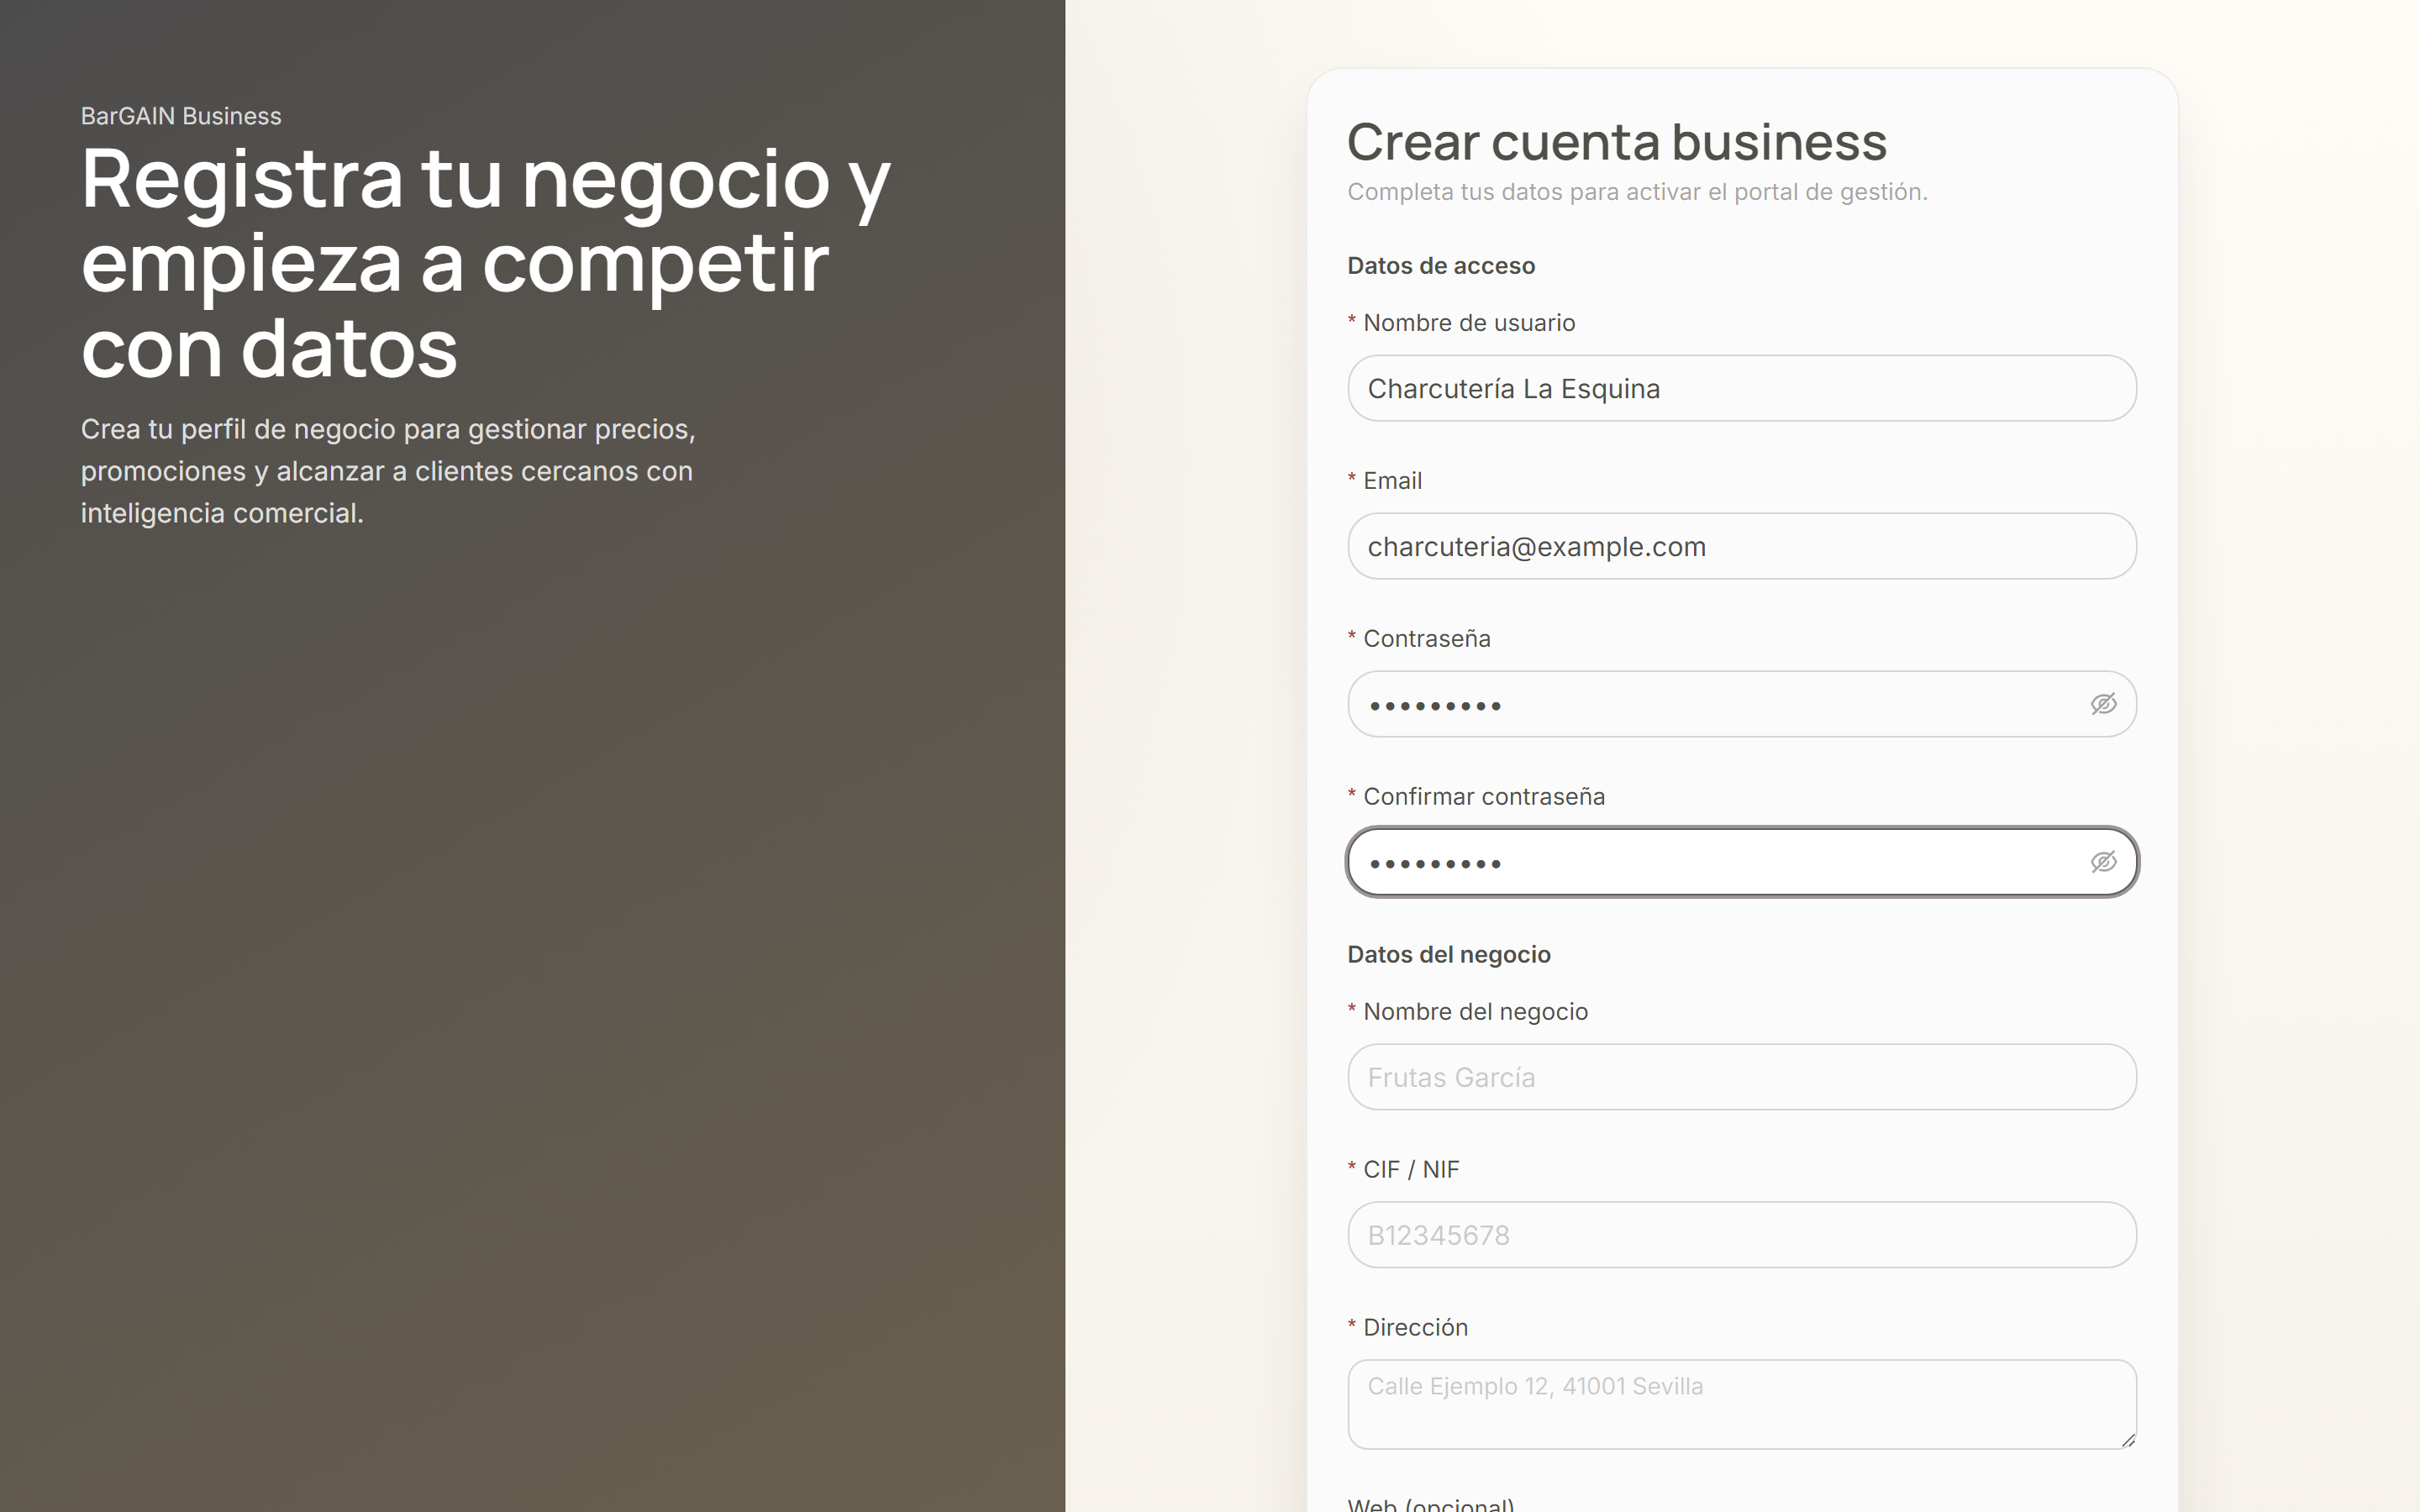
\includegraphics[width=0.46\textwidth]{diagramas/capturas/pyme-registro.png}
\caption{Portal PYME --- Inicio de sesi\'on (izquierda) y registro (derecha)}
\label{fig:cap-pyme-acceso}
\end{figure}

\begin{figure}[htbp]
\centering
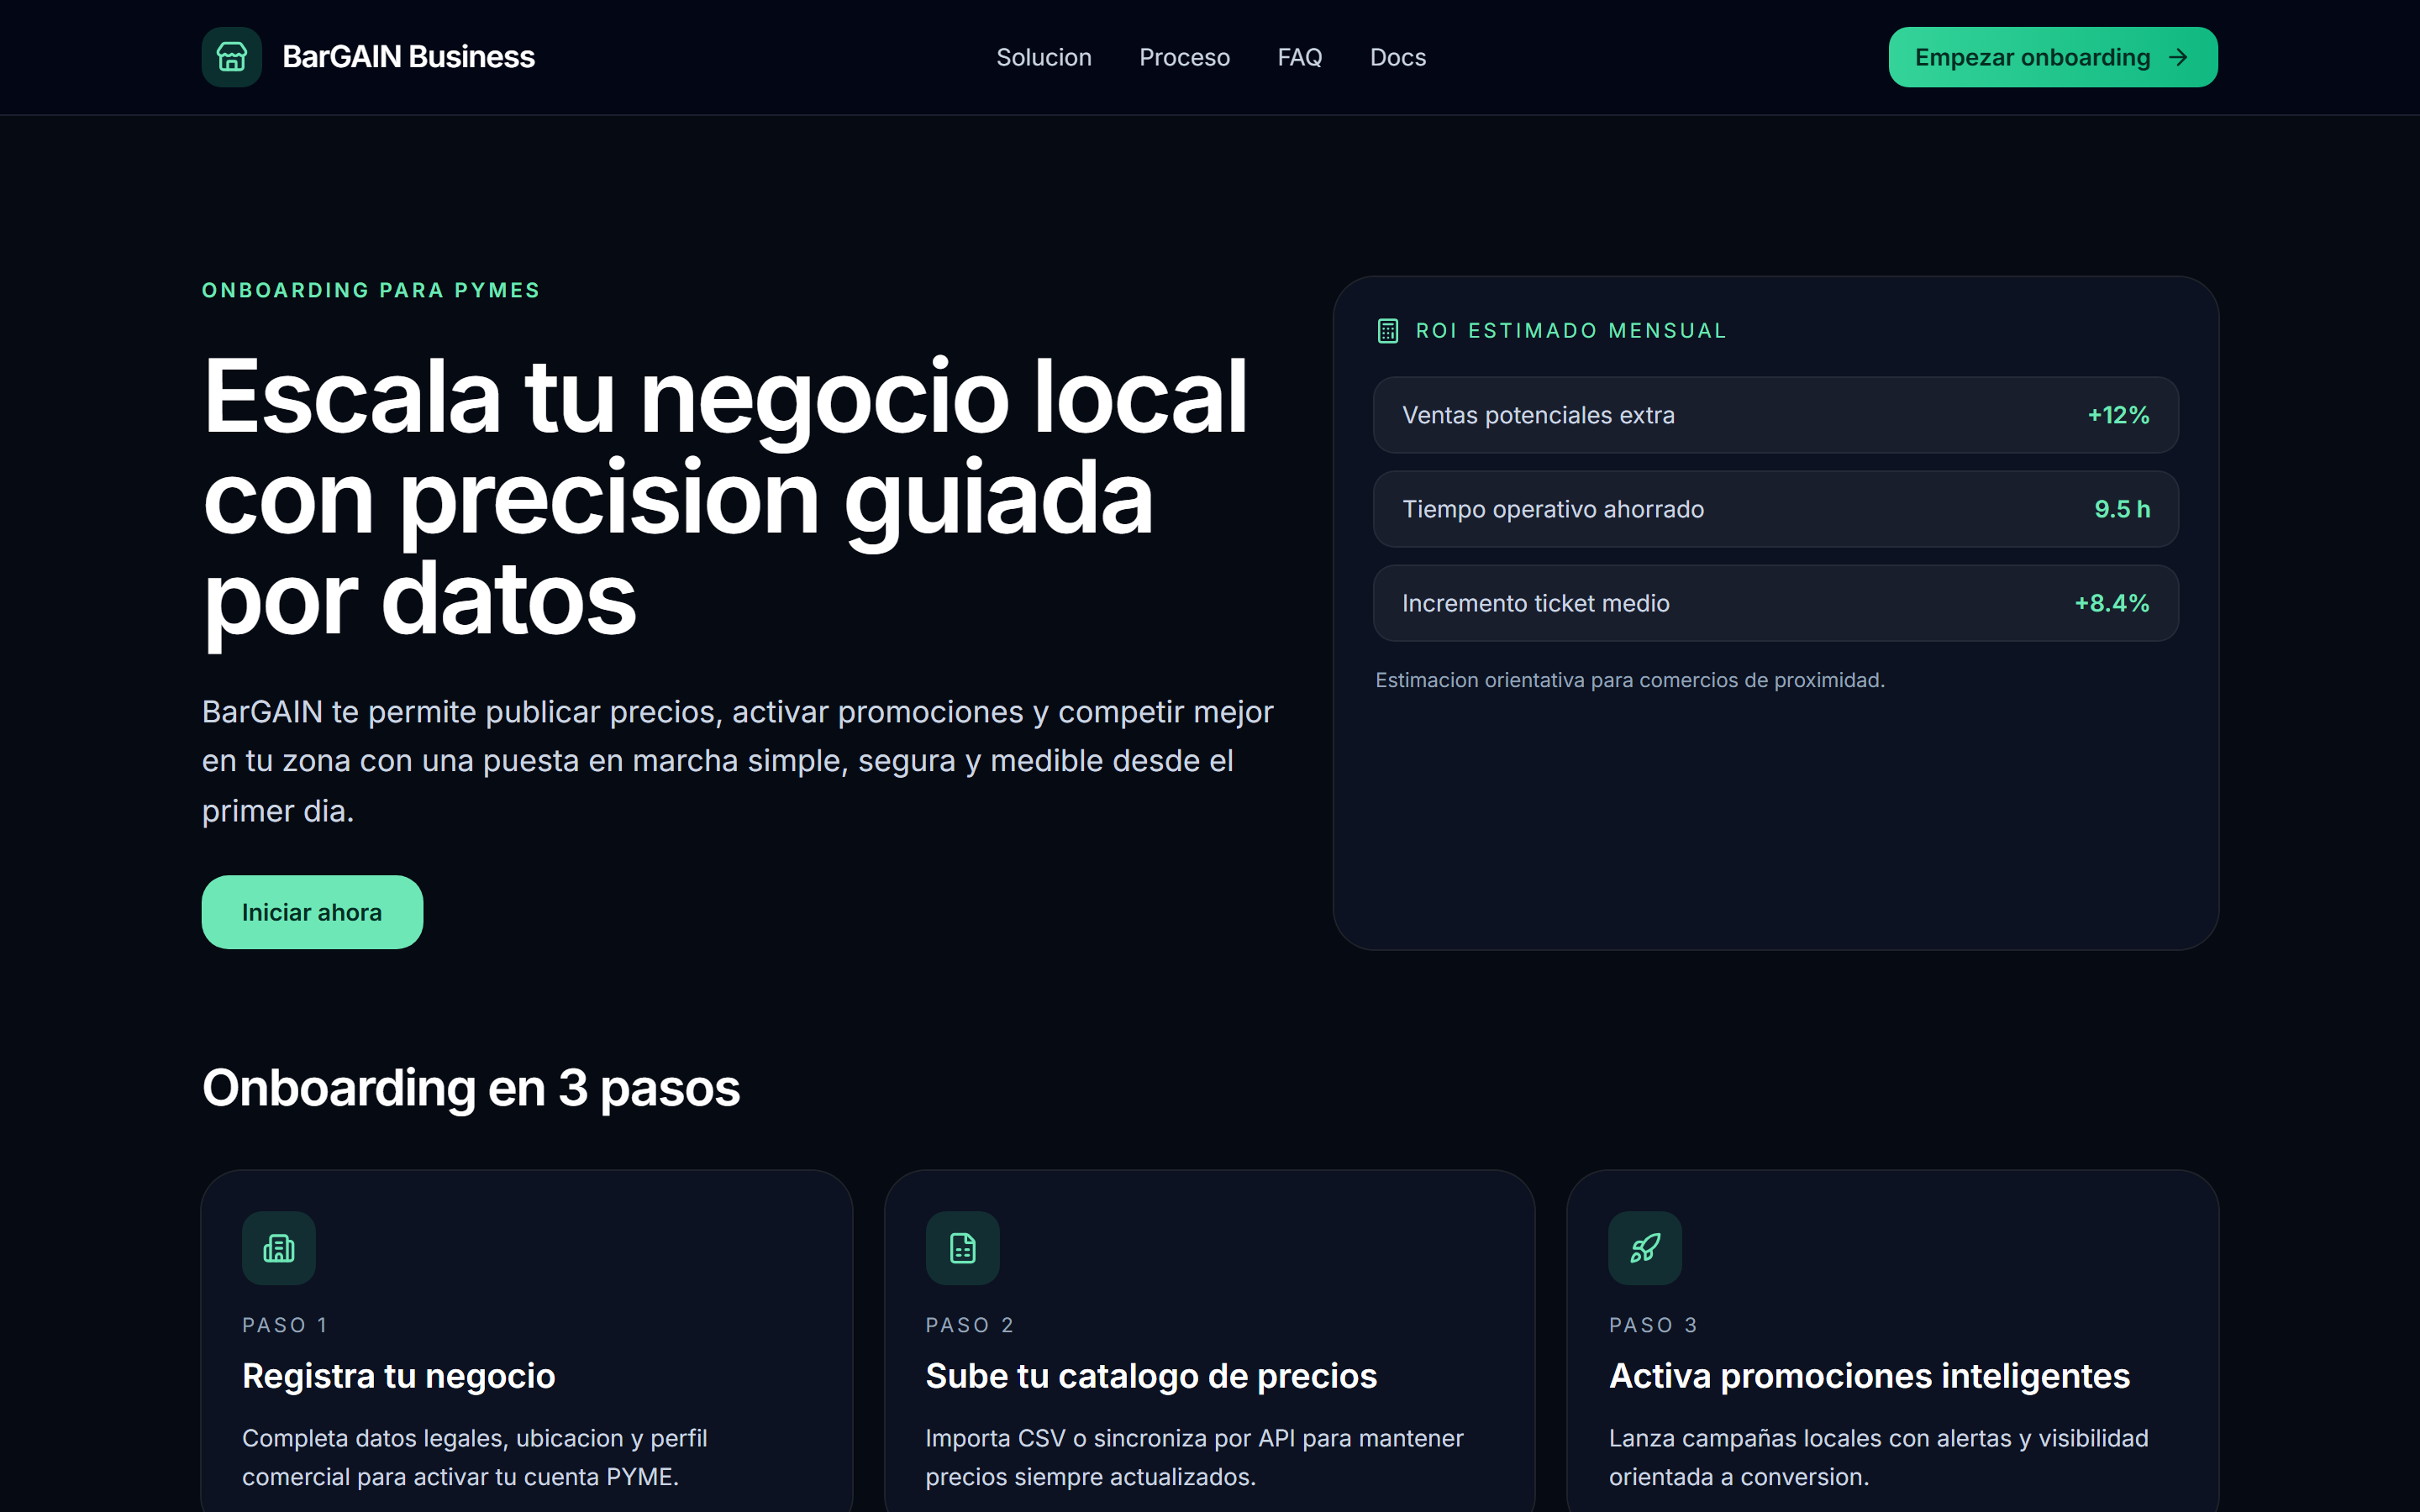
\includegraphics[width=0.85\textwidth]{diagramas/capturas/pyme-onboarding.png}
\caption{Portal PYME --- Onboarding del negocio (alta de datos y CIF)}
\label{fig:cap-pyme-onboarding}
\end{figure}

\begin{figure}[htbp]
\centering
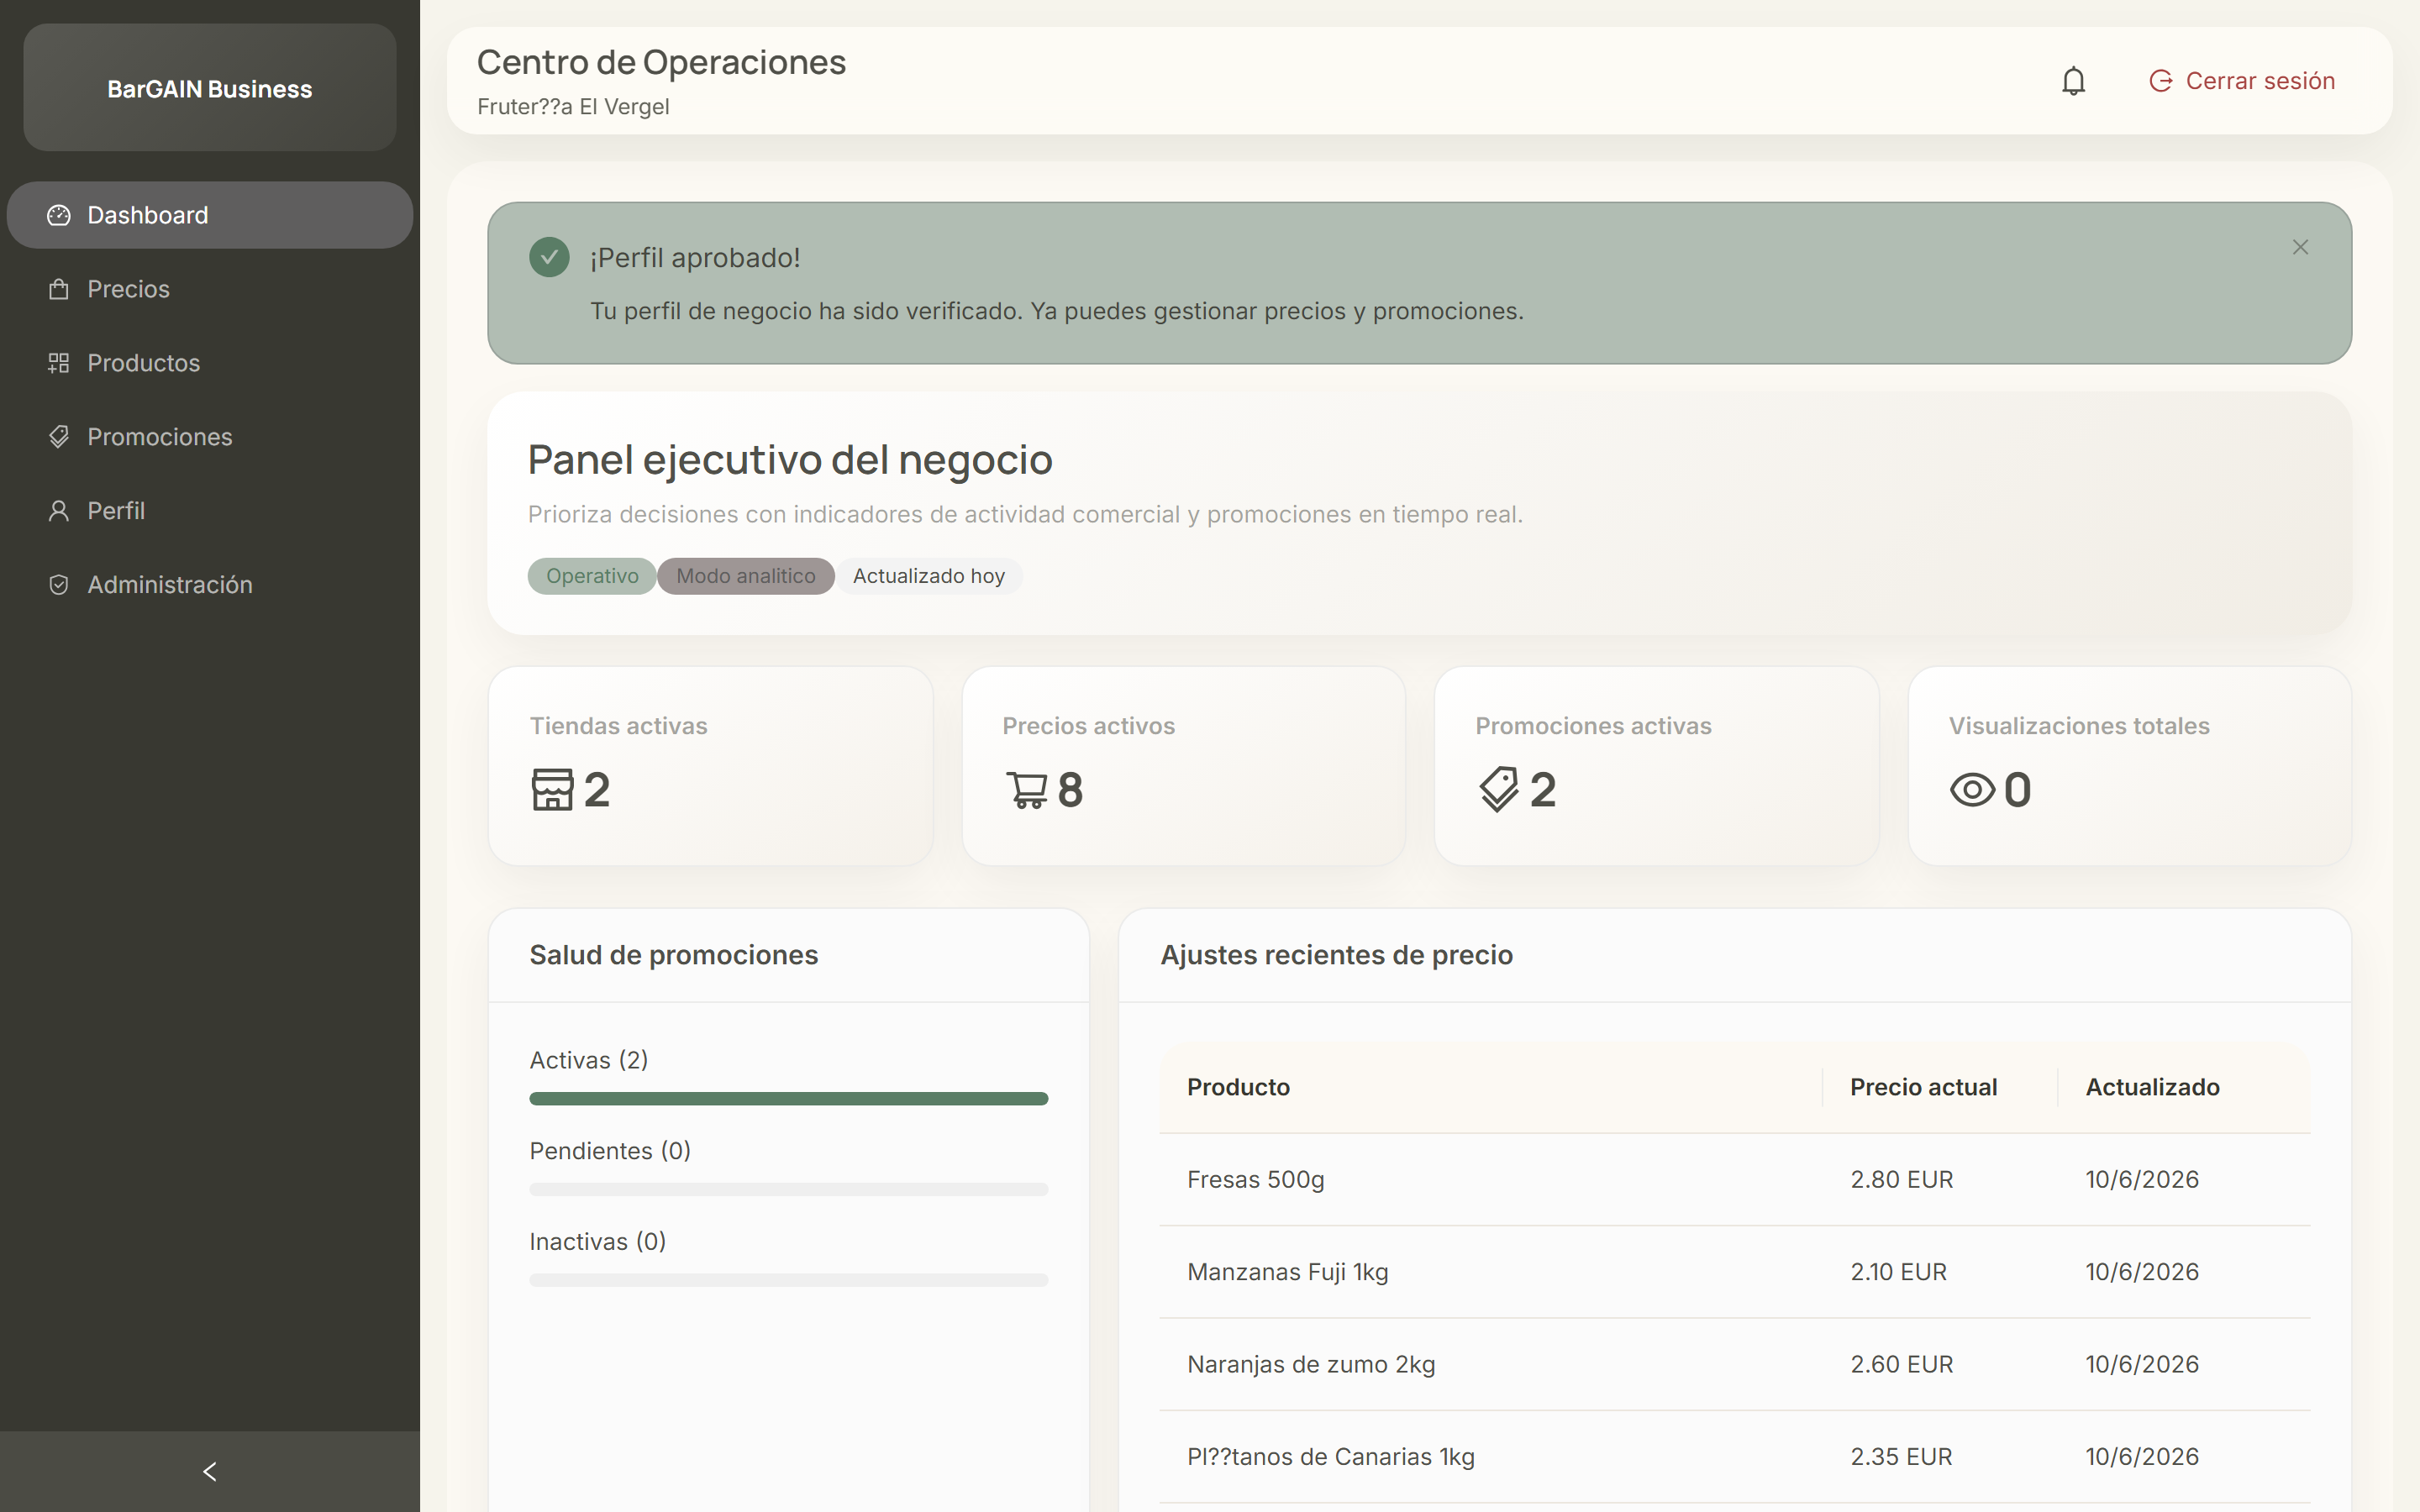
\includegraphics[width=0.85\textwidth]{diagramas/capturas/pyme-dashboard.png}
\caption{Portal PYME --- Panel de control (\emph{dashboard}) con estad\'isticas}
\label{fig:cap-pyme-dashboard}
\end{figure}

\clearpage

\begin{figure}[htbp]
\centering
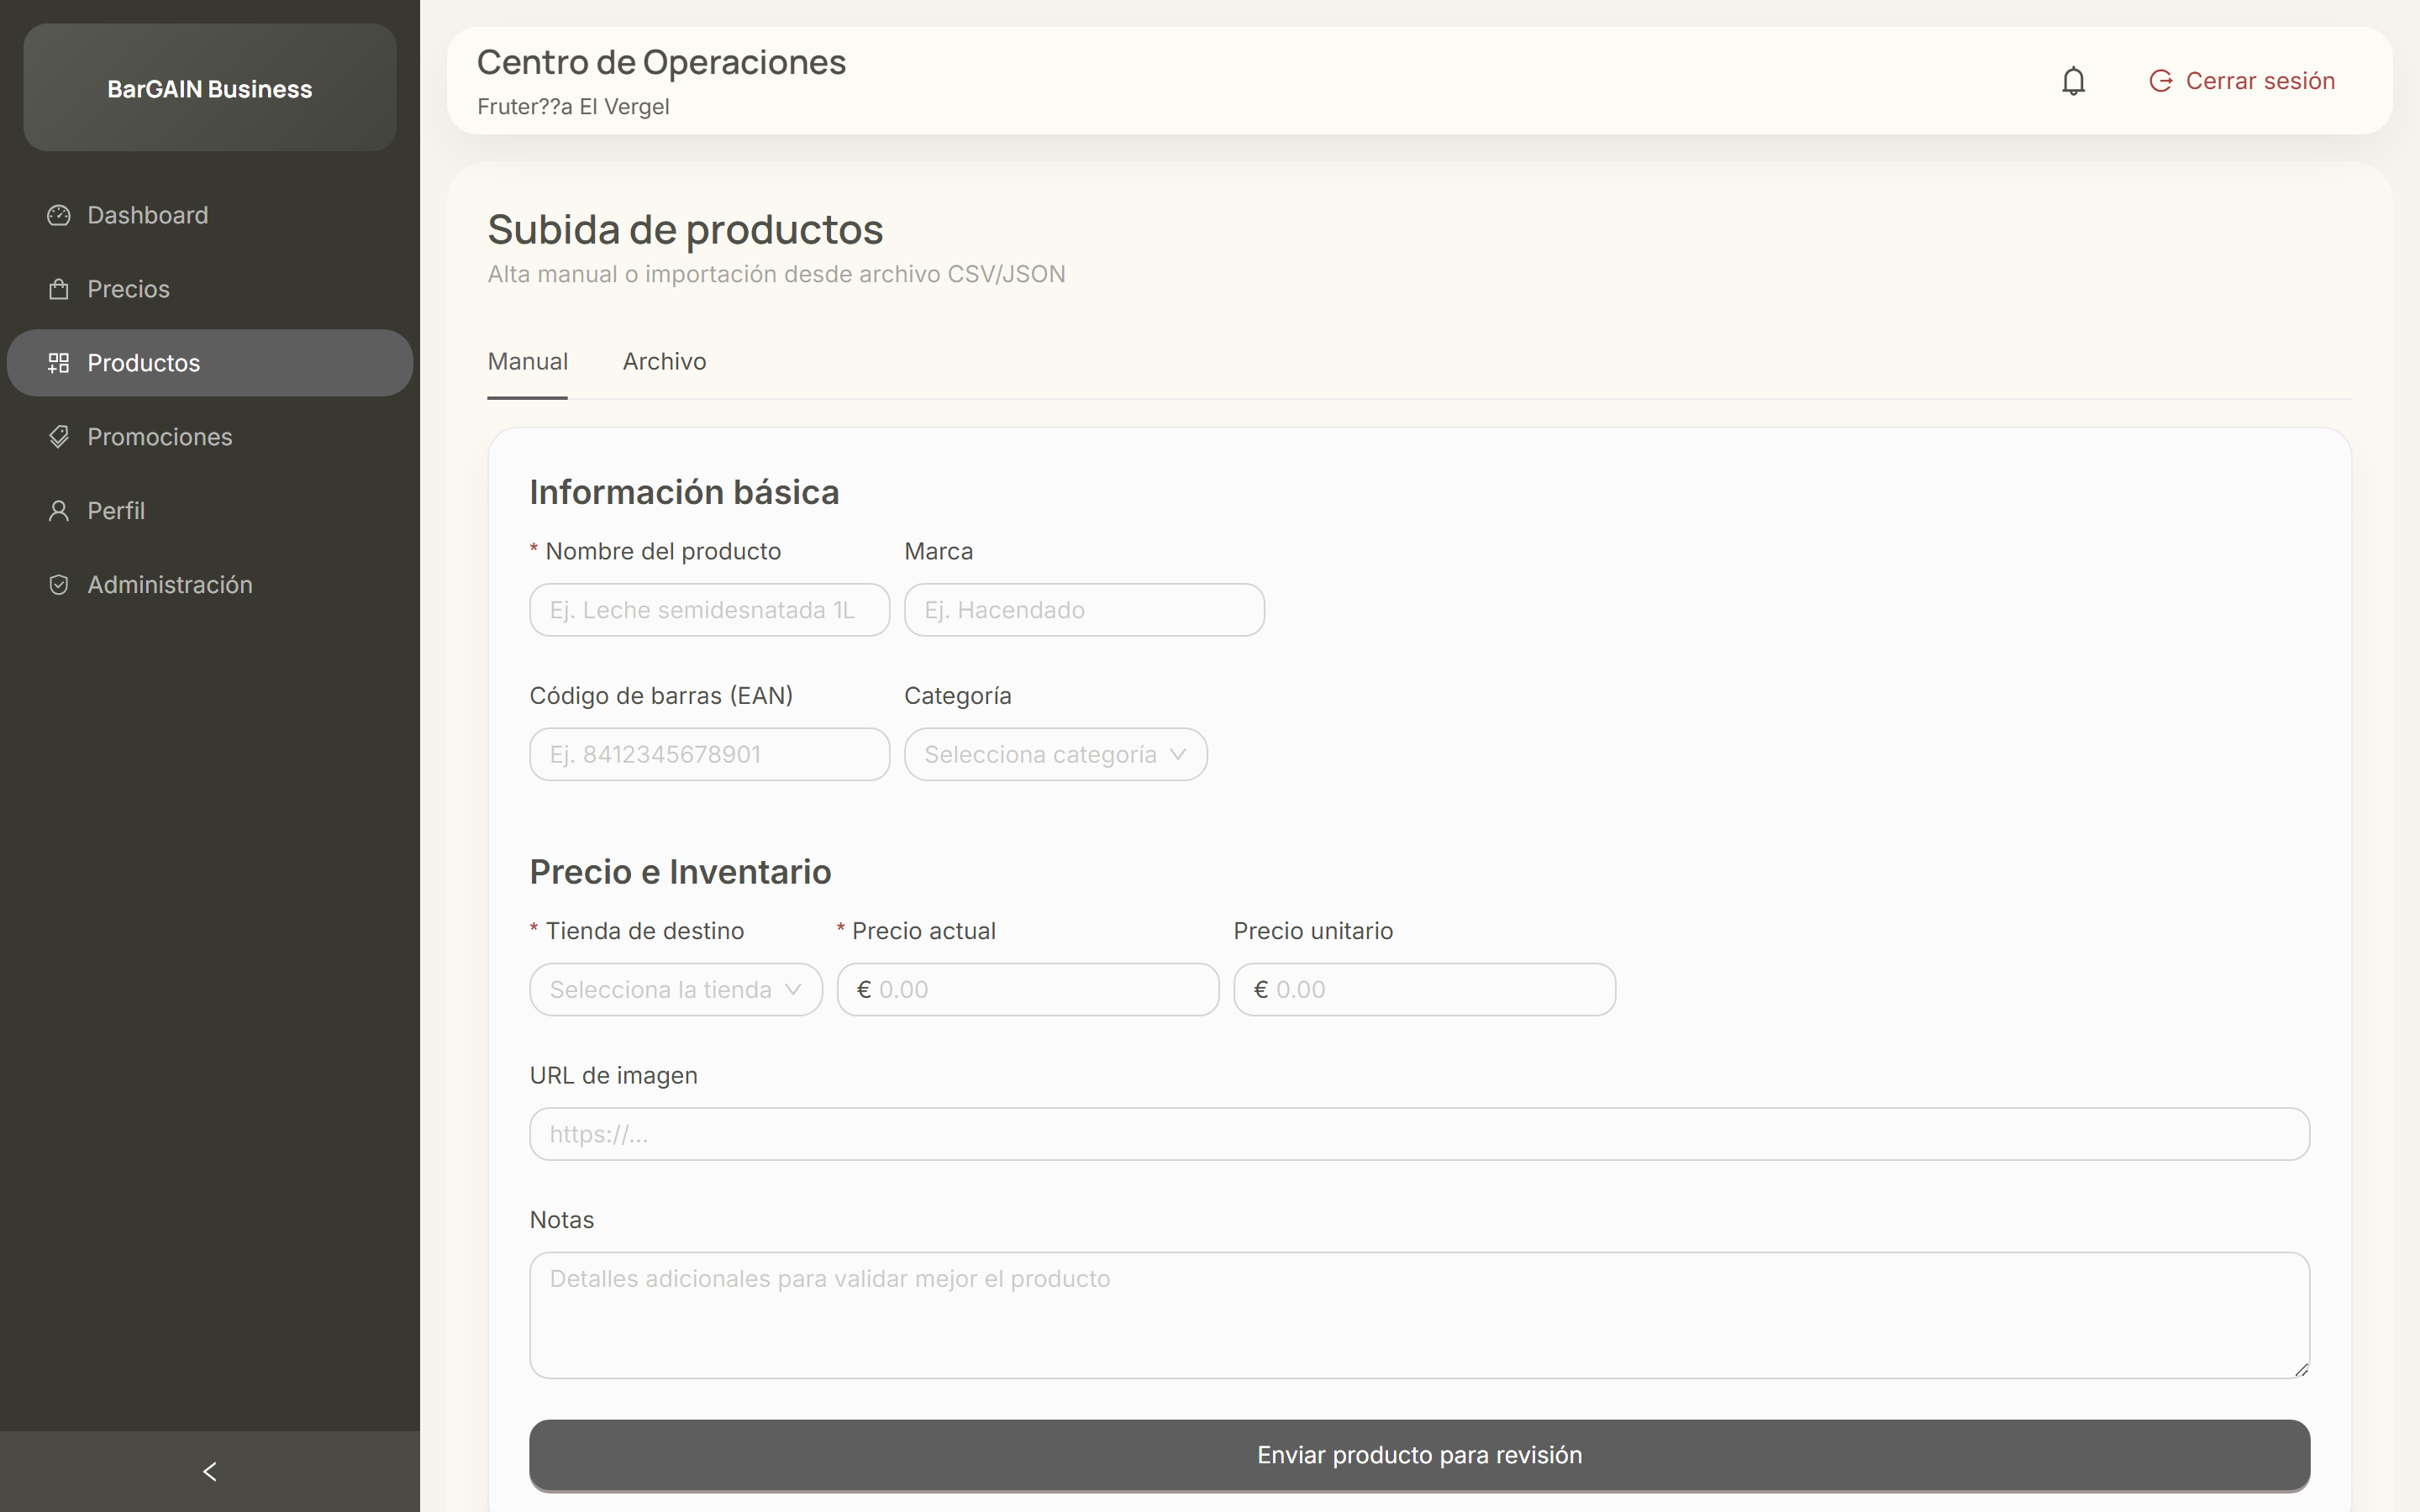
\includegraphics[width=0.46\textwidth]{diagramas/capturas/pyme-productos.png}
\hfill
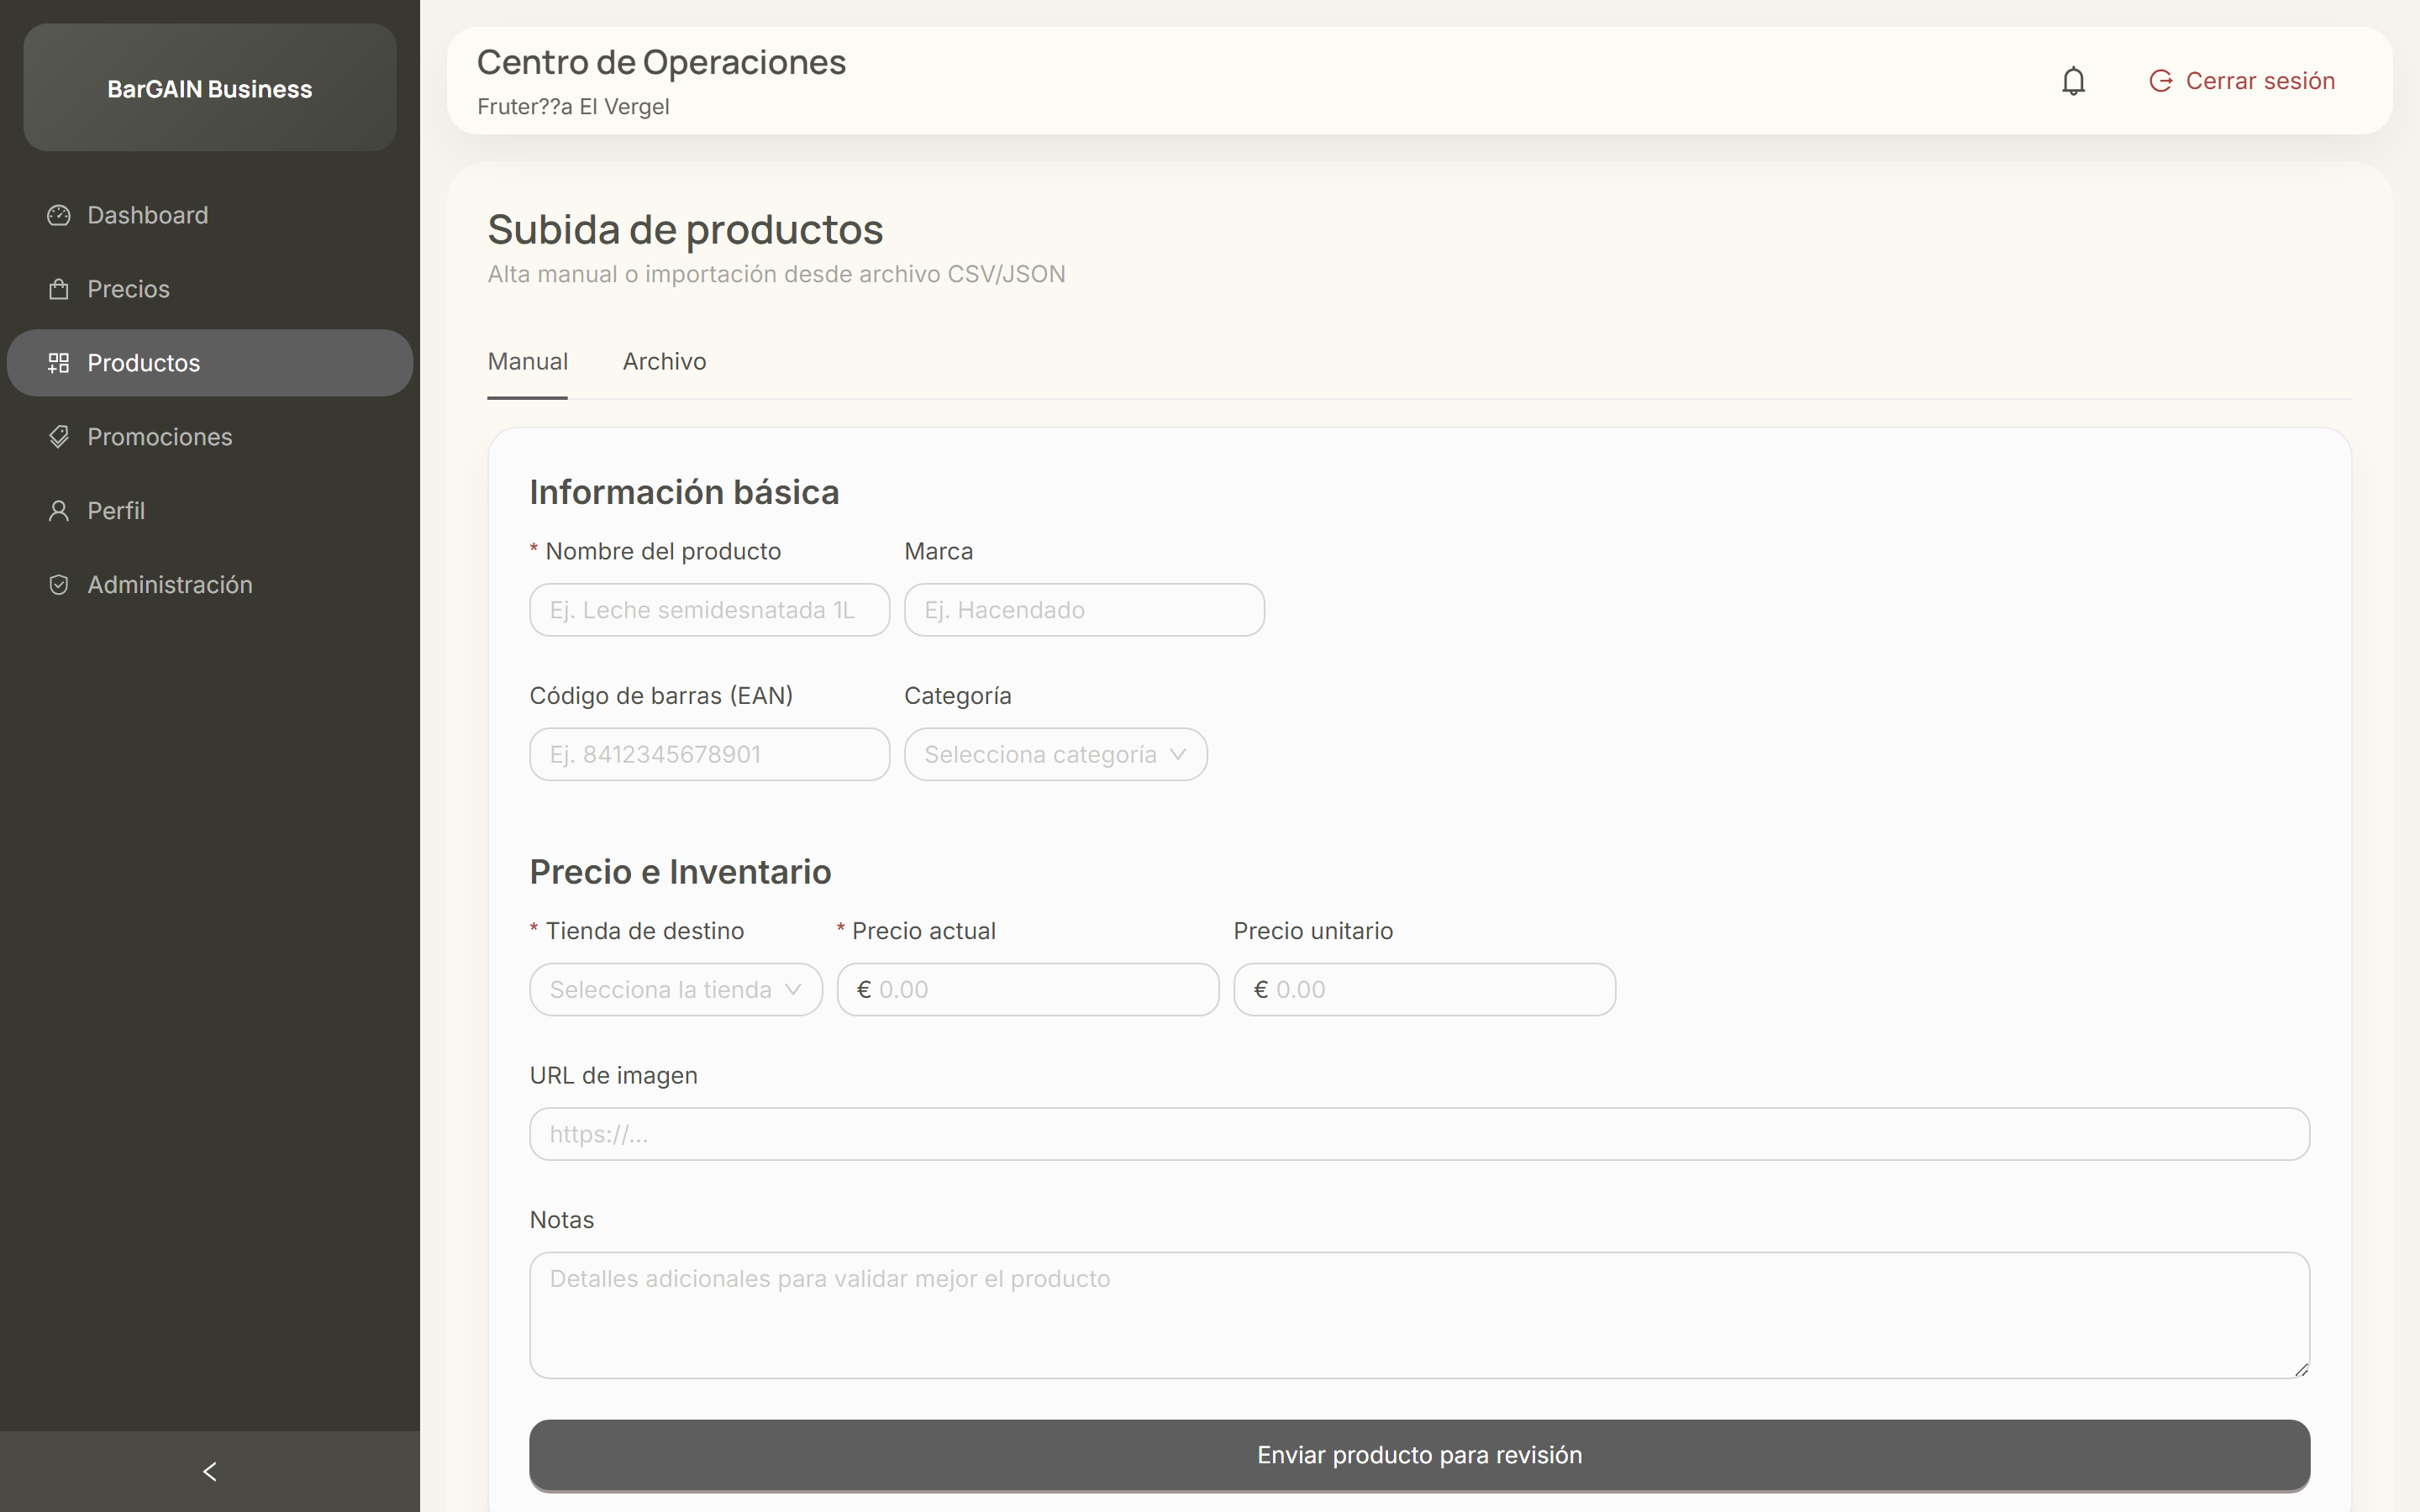
\includegraphics[width=0.46\textwidth]{diagramas/capturas/pyme-carga-masiva.png}
\caption{Portal PYME --- Gesti\'on de productos (izquierda) y carga masiva por CSV (derecha)}
\label{fig:cap-pyme-productos}
\end{figure}

\begin{figure}[htbp]
\centering
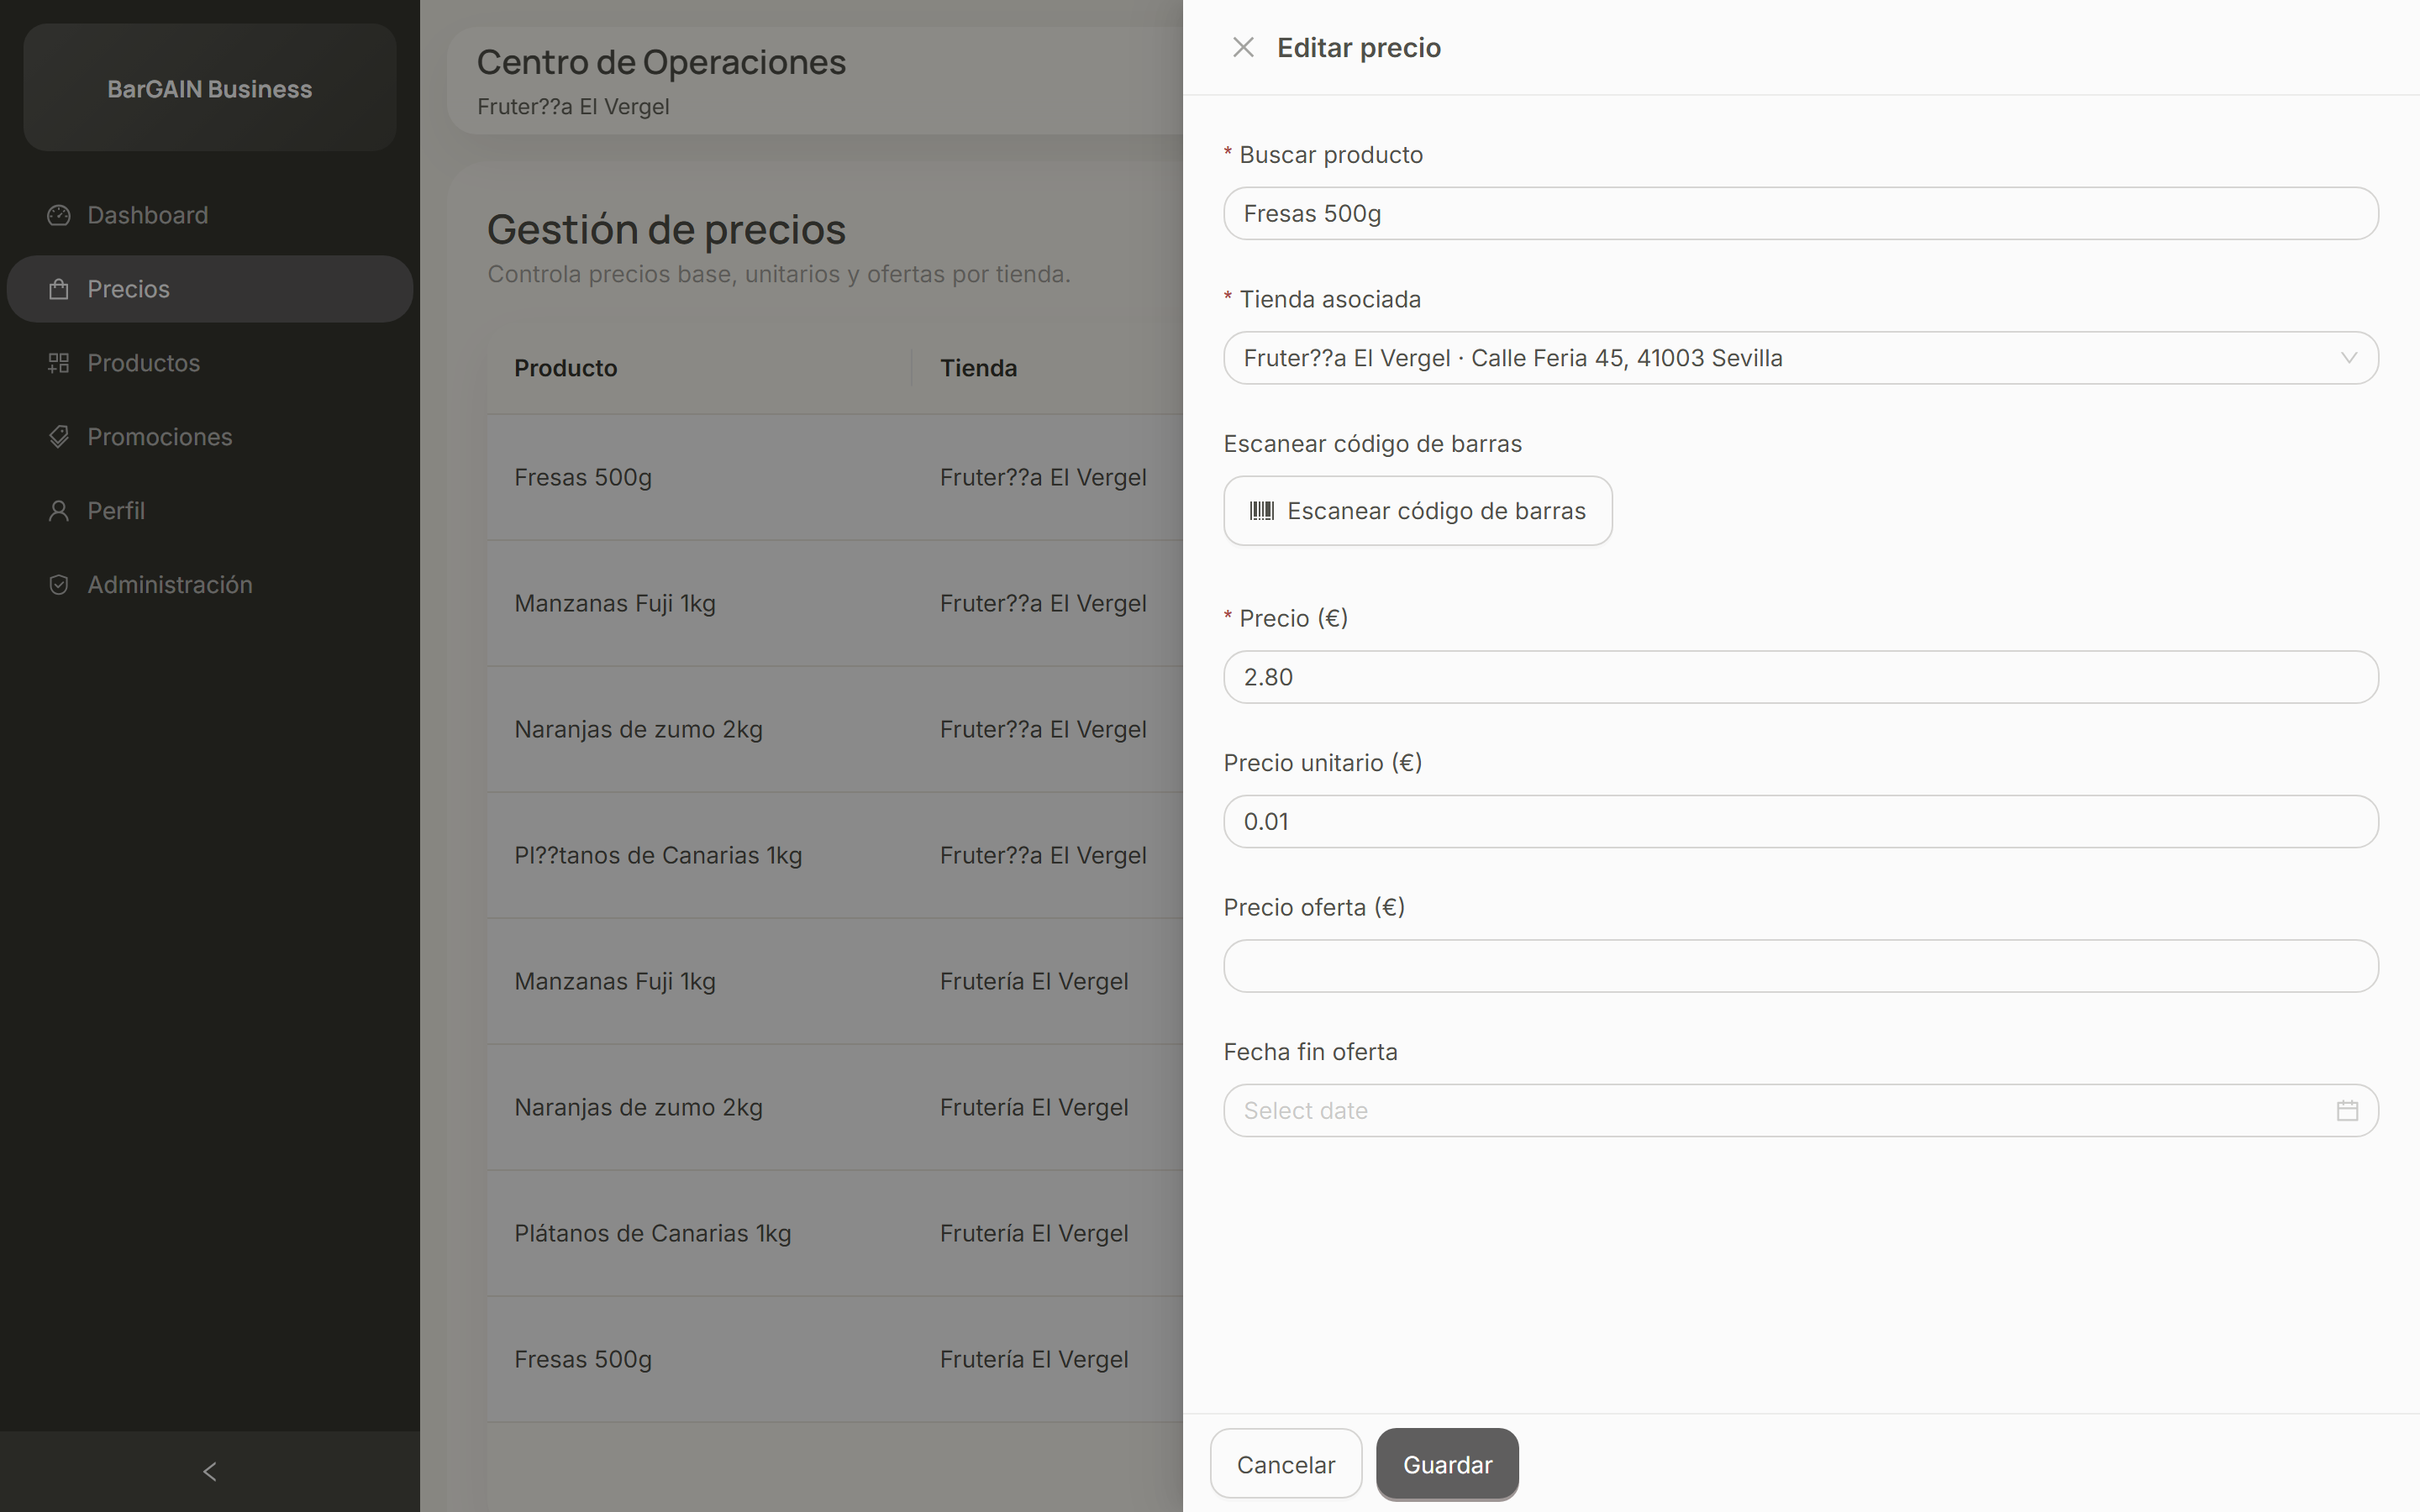
\includegraphics[width=0.85\textwidth]{diagramas/capturas/pyme-precios.png}
\caption{Portal PYME --- Gesti\'on de precios (tabla editable)}
\label{fig:cap-pyme-precios}
\end{figure}

\begin{figure}[htbp]
\centering
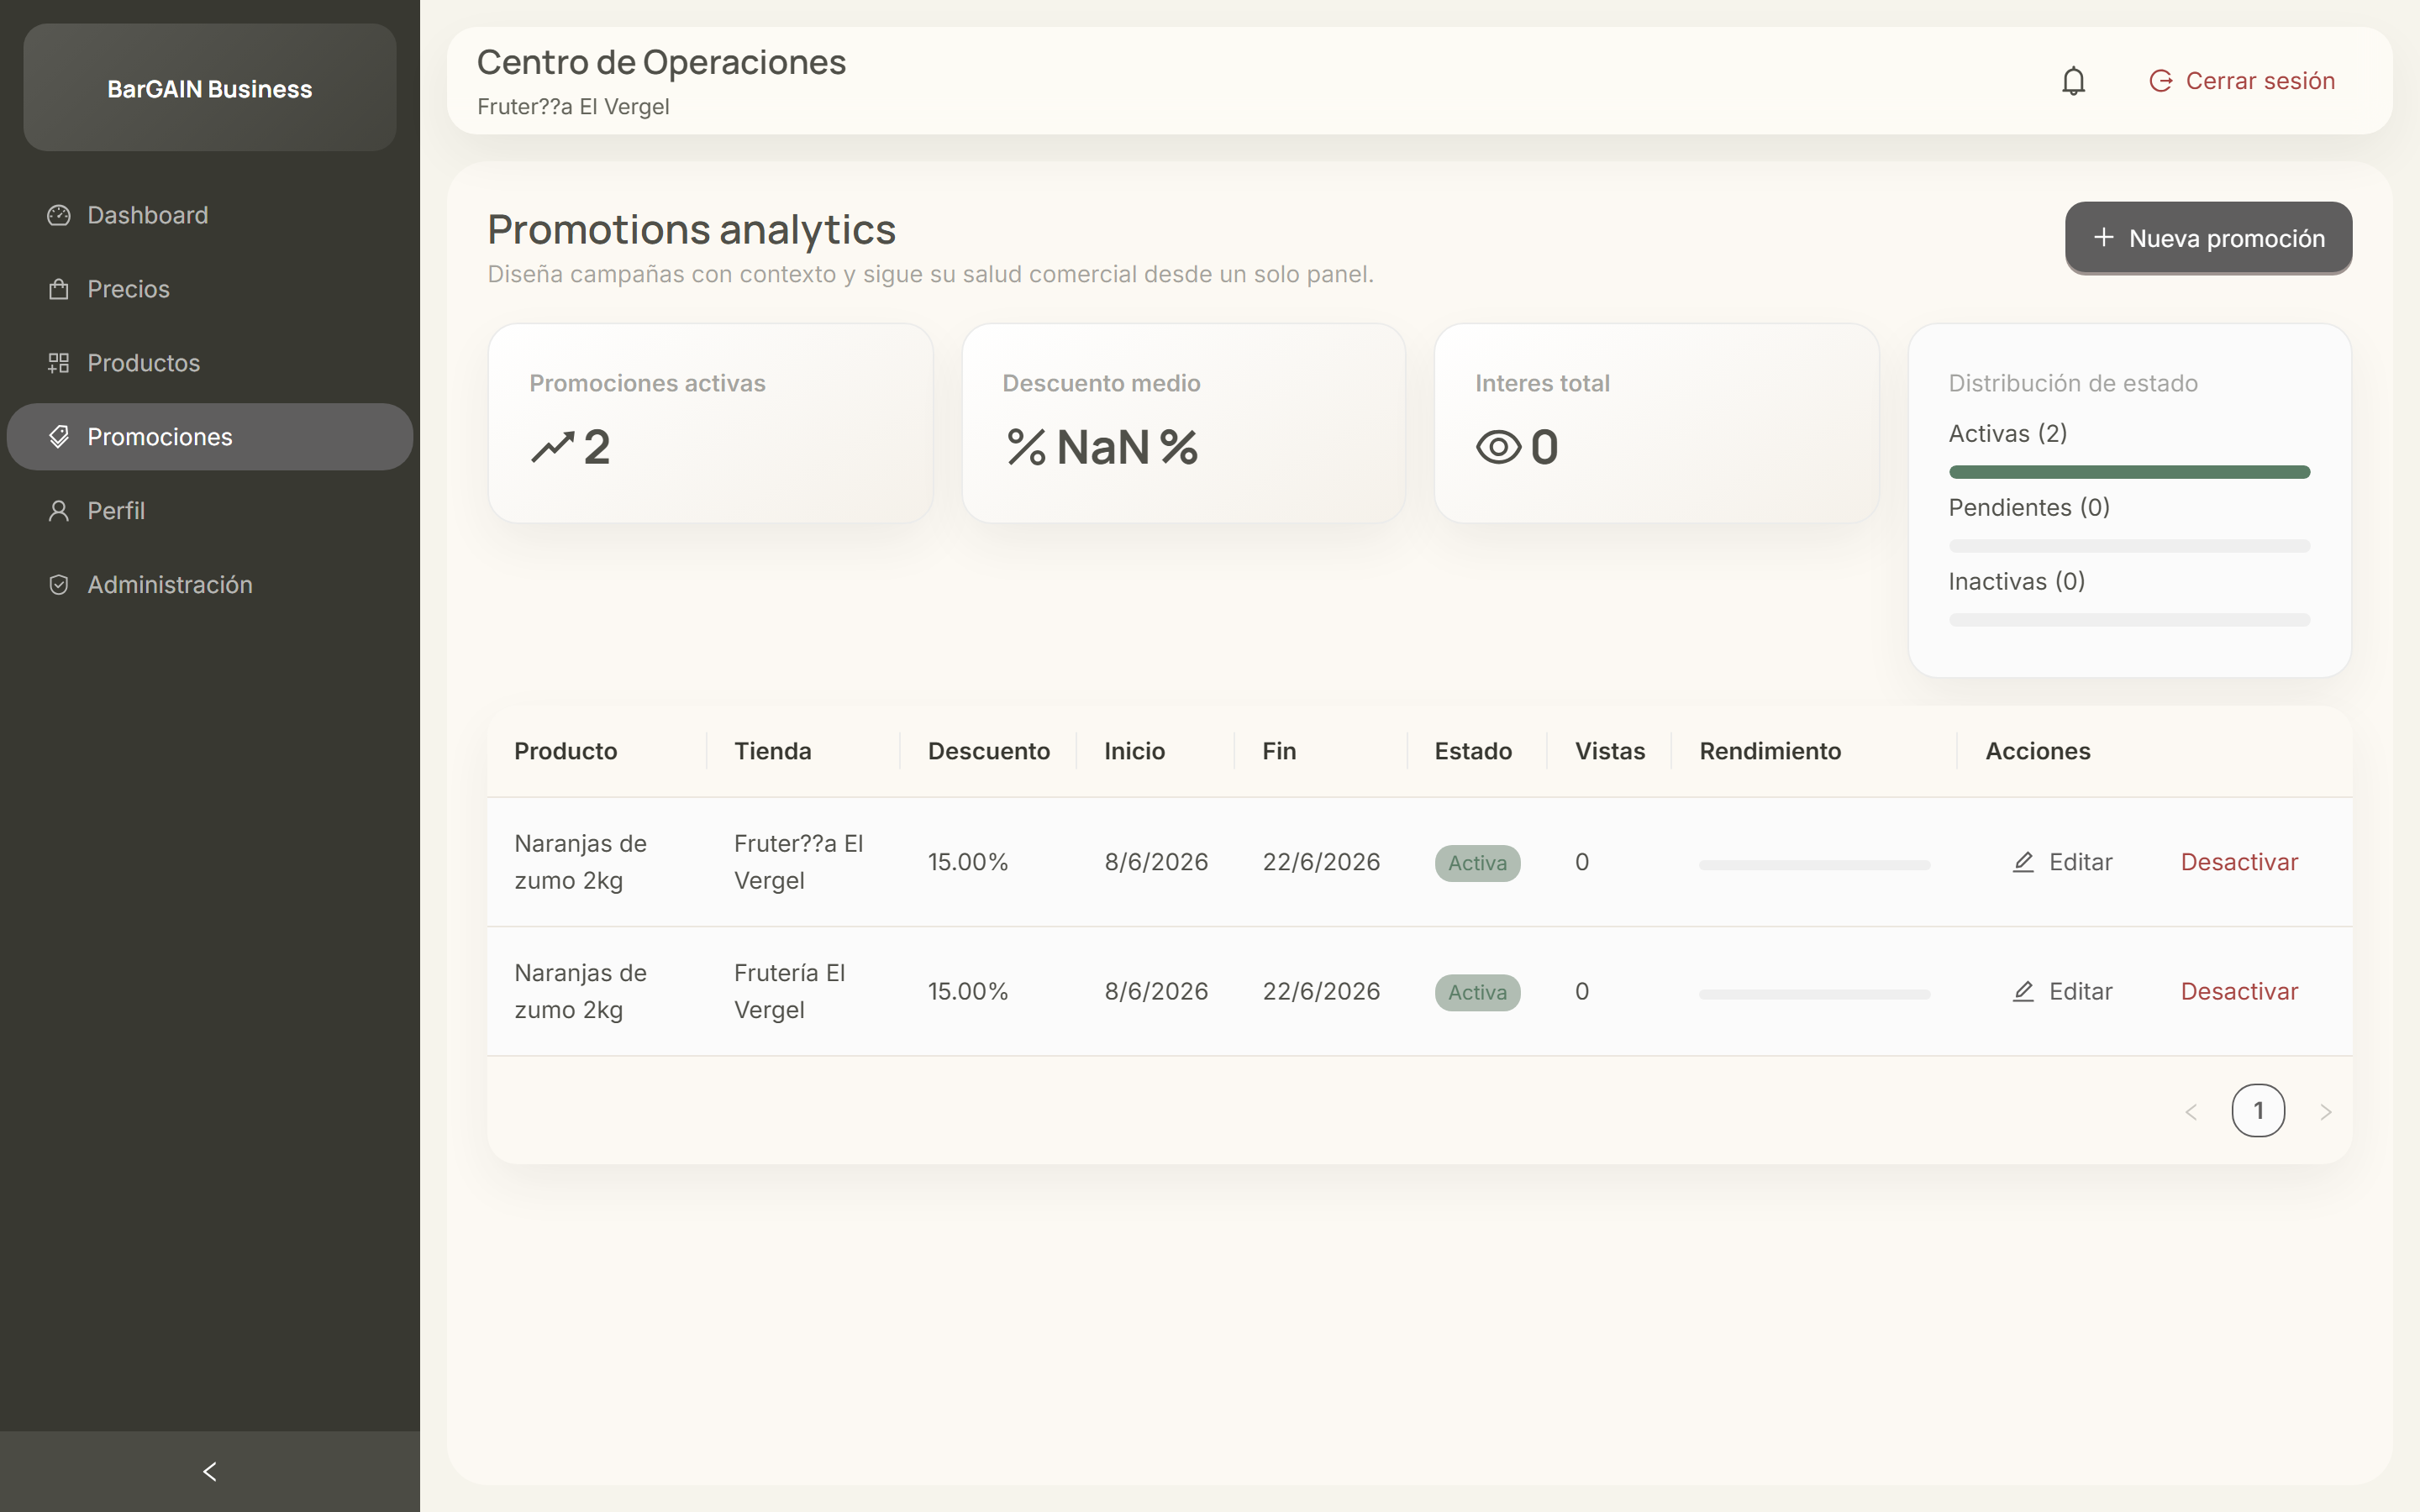
\includegraphics[width=0.46\textwidth]{diagramas/capturas/pyme-promociones.png}
\hfill
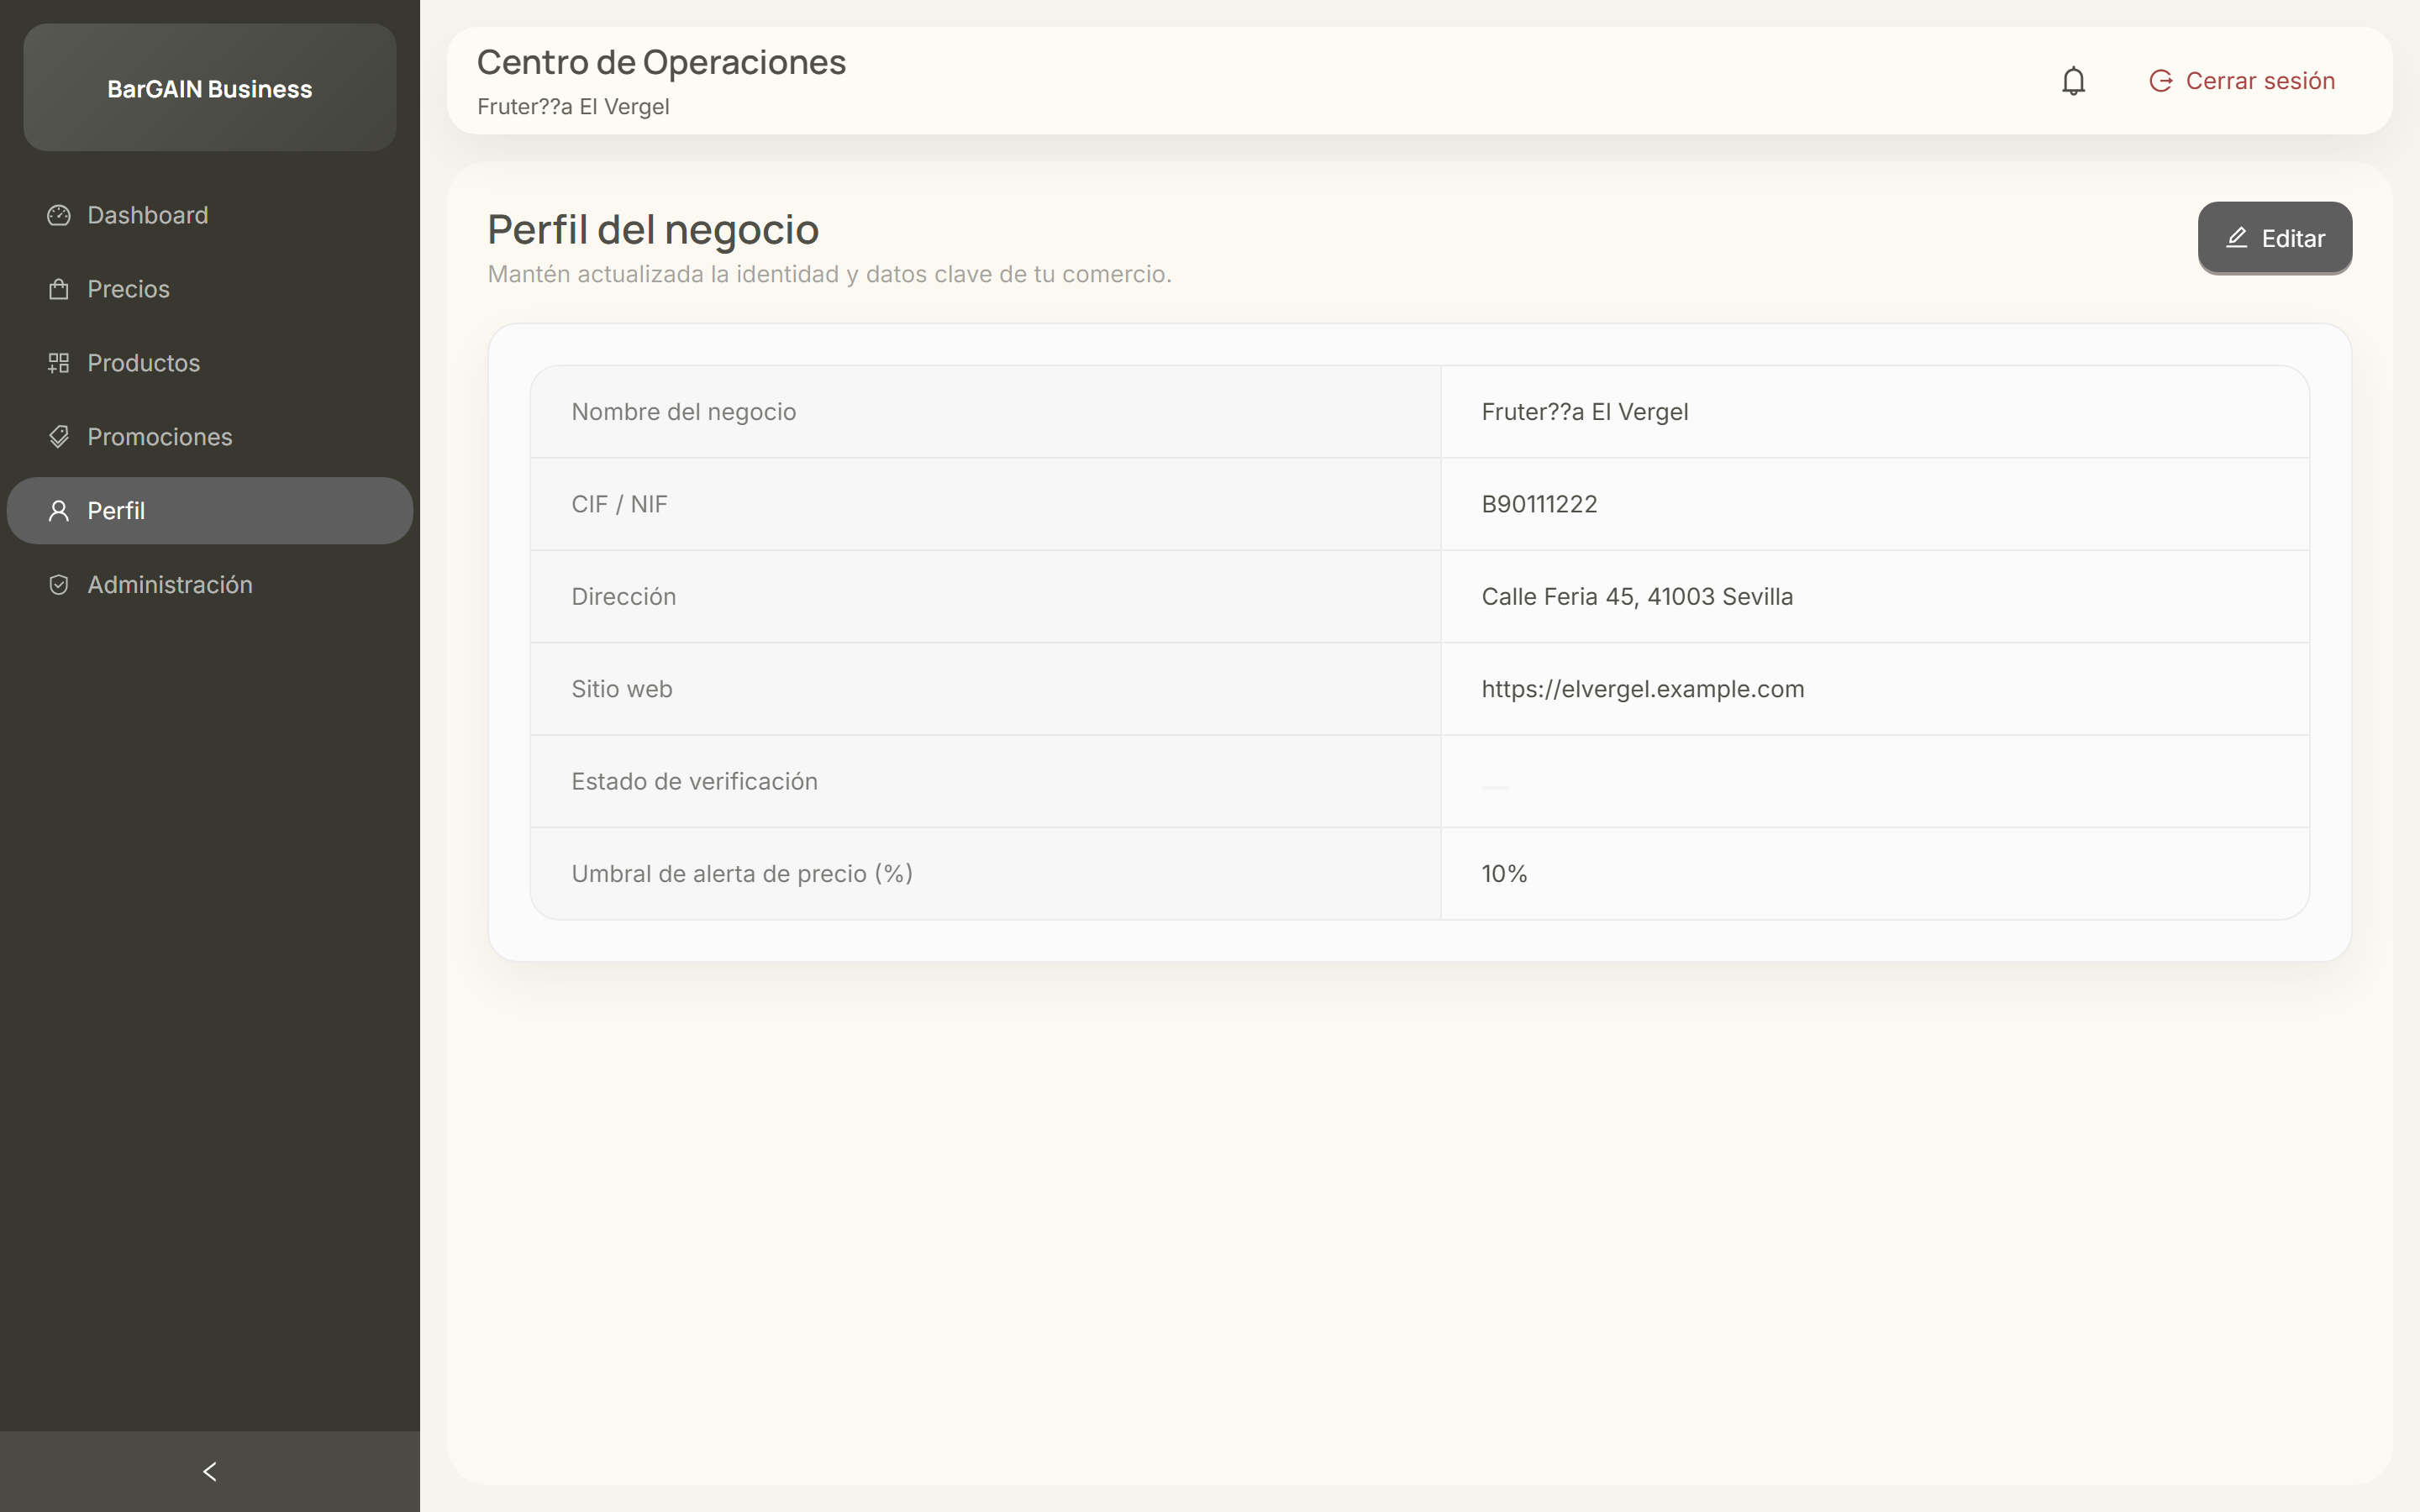
\includegraphics[width=0.46\textwidth]{diagramas/capturas/pyme-perfil-negocio.png}
\caption{Portal PYME --- Gesti\'on de promociones (izquierda) y perfil del negocio (derecha)}
\label{fig:cap-pyme-promo-perfil}
\end{figure}

\begin{figure}[htbp]
\centering
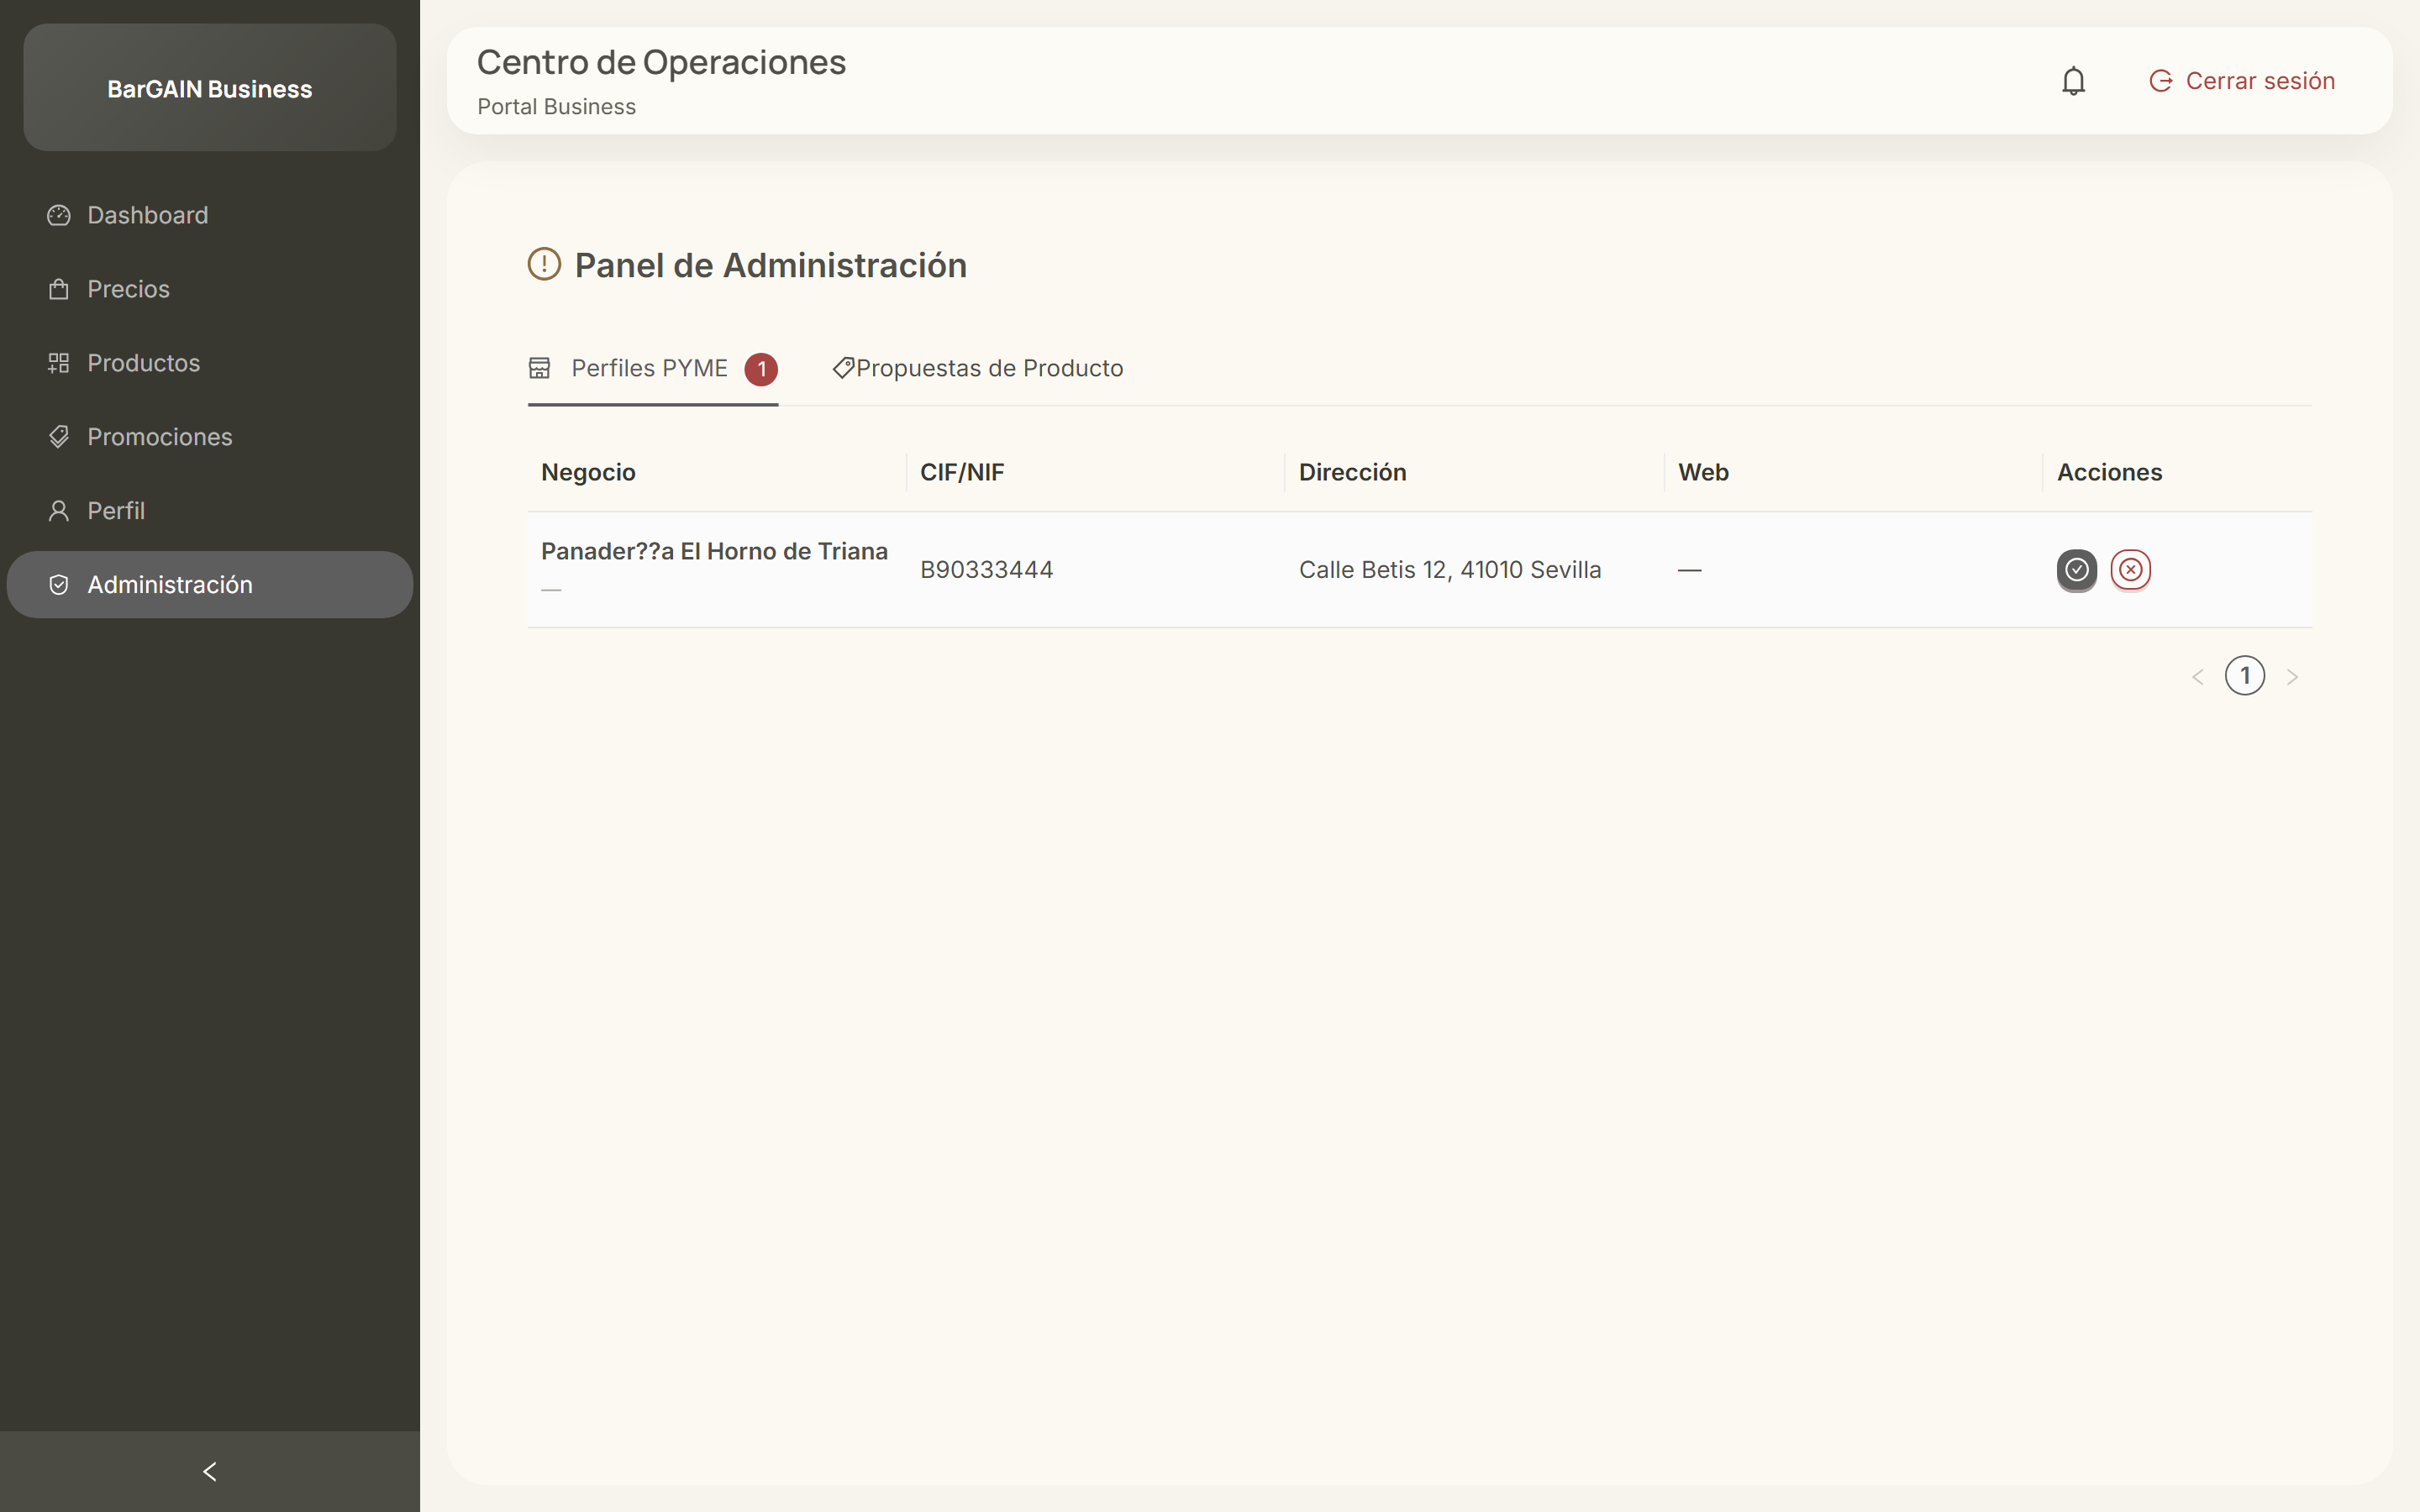
\includegraphics[width=0.85\textwidth]{diagramas/capturas/pyme-admin-aprobacion.png}
\caption{Portal PYME --- Aprobaci\'on de negocios por el administrador}
\label{fig:cap-pyme-admin}
\end{figure}

\clearpage

\section{Resoluci\'on de incidencias comunes}\label{sec:manual-incidencias}

\begin{itemize}
  \item \textbf{Frontend no conecta con backend:} verificar que el backend est\'a levantado
    (\texttt{make dev}) y expuesto en \texttt{http://localhost:8000}.
  \item \textbf{Errores JWT al navegar:} cerrar sesi\'on e iniciar de nuevo para regenerar
    credenciales.
  \item \textbf{No aparecen tiendas en mapa:} comprobar permisos de ubicaci\'on del dispositivo
    o usar coordenadas v\'alidas desde preferencias de perfil.
  \item \textbf{OCR no reconoce texto:} asegurarse de que hay buena iluminaci\'on y el texto es
    legible; usar la opci\'on de galer\'ia con una foto de mayor calidad.
  \item \textbf{Optimizaci\'on muy lenta:} la primera optimizaci\'on tras arrancar el backend puede
    tardar hasta 30 s (cold start en Render free tier). Las siguientes son instant\'aneas porque
    el worker Celery est\'a caliente.
\end{itemize}

     % !TEX root = ../proyect.tex

\chapter{Pruebas y Resultados}\label{cap10}

\section{Objetivo}\label{sec:pruebas-objetivo}

Validar que BargAIn cumple los requisitos funcionales y no funcionales definidos en la Fase de
An\'alisis, con cobertura autom\'atica de los flujos cr\'iticos y verificaci\'on documentada de los
requisitos no funcionales clave (RNF-002, RNF-004, RNF-005).

\section{Estrategia de testing}\label{sec:estrategia}

Se aplica una estrategia por capas, siguiendo el modelo de pir\'amide de tests:

\begin{itemize}
  \item \textbf{Tests unitarios backend:} por m\'odulo (\texttt{users}, \texttt{products},
    \texttt{stores}, \texttt{prices}, \texttt{shopping\_lists}, \texttt{business},
    \texttt{notifications}, \texttt{optimizer}).
  \item \textbf{Tests de integraci\'on backend:} flujos cross-domain que ejercitan varios m\'odulos
    en conjunto.
  \item \textbf{Tests de componentes frontend:} Jest + React Native Testing Library
    (111 tests en 16 suites), incluyendo los componentes y utilidades de la adaptaci\'on web.
  \item \textbf{Tests E2E con Playwright:} 4 flujos cr\'iticos del sistema integrado
    (backend + frontend web).
  \item \textbf{UAT manual en dispositivo m\'ovil:} flujos nativos con GPS y c\'amara que no son
    automatizables mediante Playwright (verificados en iPhone con la app compilada).
\end{itemize}

\section{Entorno de ejecuci\'on}\label{sec:entorno-pruebas}

\begin{itemize}
  \item \textbf{Backend:} ejecuci\'on dentro del contenedor Docker (modelo h\'ibrido ADR-002).
    Pytest con configuraci\'on en \texttt{backend/pytest.ini},
    \texttt{DJANGO\_SETTINGS\_MODULE = config.settings.test}.
  \item \textbf{E2E Playwright:} ejecuci\'on nativa en host (no Docker) contra el backend Docker
    local o el staging de Render. Instalado en \texttt{frontend/web/} como dependencia de
    desarrollo.
\end{itemize}

Los comandos de ejecuci\'on principales son:

\begin{verbatim}
# Backend (desde raiz del repo)
make test-backend           # Tests con -v --tb=short
make test-backend-cov       # Con cobertura HTML

# E2E (desde host)
cd frontend/web && npx playwright test
cd frontend/web && npx playwright test --reporter=html
\end{verbatim}

\section{Suite de tests backend}\label{sec:suite-backend}

\subsection{Tests de integraci\'on}\label{subsec:tests-integracion}

Los tests de integraci\'on verifican flujos API completos usando una base de datos de test real
(sin mocks de BD), validando el comportamiento end-to-end del backend.

\begin{table}[h]
\caption{Suite de tests de integraci\'on backend}
\label{tab:tests-integracion}
\centering
\begin{tabular}{|l|l|l|}
\hline
\textbf{Archivo de test} & \textbf{M\'odulo} & \textbf{Descripci\'on} \\
\hline
\texttt{test\_auth\_endpoints.py} & users & Registro, login, refresh, perfil \\
\texttt{test\_optimizer\_api.py} & optimizer & POST /optimize/ con matriz mock \\
\texttt{test\_ocr\_api.py} & ocr & POST /ocr/scan/ con Vision API mock \\
\texttt{test\_business\_verification.py} & business & Aprobar/rechazar BusinessProfile \\
\texttt{test\_business\_registration.py} & business & Onboarding PYME \\
\texttt{test\_business\_prices.py} & business & Gesti\'on de precios PYME \\
\texttt{test\_bulk\_prices.py} & business & Actualizaci\'on masiva CSV \\
\texttt{test\_proposal\_admin.py} & business & Aprobar/rechazar propuestas (6 tests) \\
\texttt{test\_list\_endpoints.py} & shopping\_lists & CRUD listas e \'items \\
\texttt{test\_cross\_domain.py} & core & Flujos cross-domain \\
\texttt{test\_notification\_dispatch.py} & notifications & Despacho push/email \\
\texttt{test\_notification\_events.py} & notifications & Eventos de notificaci\'on \\
\texttt{test\_price\_endpoints.py} & prices & API de precios \\
\texttt{test\_product\_endpoints.py} & products & API de productos \\
\texttt{test\_store\_endpoints.py} & stores & API de tiendas \\
\texttt{test\_assistant\_api.py} & assistant & Endpoint LLM con mock Gemini \\
\texttt{test\_promotions.py} & business & Gesti\'on de promociones \\
\hline
\end{tabular}
\end{table}

\subsection{Cobertura}\label{subsec:cobertura}

La suite backend alcanza una cobertura m\'inima del 80\% sobre los m\'odulos de aplicaci\'on
(\texttt{apps/}), medida con \texttt{pytest-cov}. Los m\'odulos con mayor densidad de tests son
\texttt{users}, \texttt{business} y \texttt{optimizer}, que concentran la l\'ogica de negocio
principal.

\section{Tests E2E con Playwright}\label{sec:playwright}

Se desarrollaron 4 tests E2E automatizados con Playwright para verificar los flujos cr\'iticos del
sistema integrado (backend + web companion Vite+React):

\begin{table}[h]
\caption{Suite de tests E2E con Playwright}
\label{tab:tests-e2e}
\centering
\begin{tabular}{|l|l|l|p{5cm}|}
\hline
\textbf{Flujo} & \textbf{Archivo} & \textbf{Tipo} & \textbf{Descripci\'on} \\
\hline
Autenticaci\'on completa & \texttt{auth.spec.ts} & UI + API &
  Registro \textrightarrow{} login \textrightarrow{} token refresh \textrightarrow{} logout \\
Lista \textrightarrow{} Optimizar \textrightarrow{} Ruta & \texttt{optimizer.spec.ts} & API-level &
  Crear lista \textrightarrow{} a\~nadir \'items \textrightarrow{} optimizar \textrightarrow{}
  verificar resultado \\
OCR ticket \textrightarrow{} lista & \texttt{ocr.spec.ts} & API-level &
  Subir imagen \textrightarrow{} endpoint OCR \textrightarrow{} respuesta estructurada \\
Business portal & \texttt{business.spec.ts} & UI &
  Registro PYME \textrightarrow{} admin aprueba \textrightarrow{} PYME accede a dashboard \\
\hline
\end{tabular}
\end{table}

Los flujos de optimizador y OCR se implementan como tests API-level (usando el fixture
\texttt{request} de Playwright, sin interfaz de usuario) porque estas funcionalidades son exclusivas
de la app m\'ovil --- el web companion es un portal business y no dispone de pantallas de
consumidor. Este enfoque verifica la integraci\'on backend end-to-end de los features principales
del TFG sin requerir una interfaz web que no existe.

\subsection{Configuraci\'on Playwright}\label{subsec:playwright-config}

\begin{itemize}
  \item \textbf{Ubicaci\'on:} \texttt{frontend/web/playwright.config.ts}
  \item \textbf{Target:} web companion en \texttt{http://localhost:5173} (o
    \texttt{PLAYWRIGHT\_BASE\_URL})
  \item \textbf{Backend:} Docker local o staging Render (\texttt{PLAYWRIGHT\_API\_URL})
  \item \textbf{Navegador:} Chromium (un solo proyecto para evitar duplicaci\'on de estado de BD)
  \item \textbf{Workers:} 1 (secuencial --- los tests comparten la misma base de datos)
\end{itemize}

\section{UAT manual en dispositivo m\'ovil}\label{sec:uat}

Los flujos que requieren APIs nativas del dispositivo (GPS, c\'amara) se verifican manualmente en
un iPhone con la app compilada mediante el workflow \texttt{ios-build.yml}:

\begin{table}[h]
\caption{Resultados UAT en dispositivo m\'ovil}
\label{tab:uat}
\centering
\begin{tabular}{|p{8cm}|c|}
\hline
\textbf{Flujo UAT} & \textbf{Resultado} \\
\hline
Solicitar ubicaci\'on y ver tiendas en mapa & Verificado \\
Crear lista y a\~nadir \'items manualmente & Verificado \\
Capturar ticket con c\'amara y reconocer productos & Verificado \\
Lanzar optimizaci\'on y navegar la ruta sugerida & Verificado \\
Chat con asistente LLM y verificar guardrail & Verificado \\
\hline
\end{tabular}
\end{table}

\section{Validaci\'on de Requisitos No Funcionales}\label{sec:nfr}

\subsection{RNF-002: Disponibilidad $\geq$ 99\% en staging}\label{subsec:rnf02}

El backend de staging se despleg\'o en Render.com (plan gratuito, blueprint
\texttt{render.free.yaml}) con la siguiente arquitectura:
\begin{itemize}
  \item Web Service \'unico: Django con Gunicorn (2 workers) y un proceso Celery
    worker + beat embebido (\texttt{--concurrency 1}) para las tareas as\'incronas.
  \item PostgreSQL 16 + PostGIS gestionado por la plataforma.
  \item Redis: broker Celery + cach\'e Google Places.
\end{itemize}

El health check se configura en \texttt{GET /api/v1/health/} respondiendo HTTP 200. Los reinicios
autom\'aticos ante fallos se gestionan por la plataforma Render. Como optimizaci\'on del arranque
en fr\'io del free tier, los ficheros est\'aticos se precompilan durante el build de la imagen
Docker en lugar de generarse en el arranque del servicio.

\subsection{RNF-004: Usabilidad WCAG 2.1 AA y m\'aximo 3 taps}\label{subsec:rnf04}

Los flujos principales se completan en \textless{}= 3 interacciones en la app m\'ovil:

\begin{itemize}
  \item \textbf{Ver precios cercanos:} Home \textrightarrow{} Buscar \textrightarrow{} Resultados
    (3 taps)
  \item \textbf{Optimizar ruta:} Lista \textrightarrow{} Optimizar \textrightarrow{} Ver ruta
    (3 taps)
  \item \textbf{A\~nadir \'item OCR:} Lista \textrightarrow{} C\'amara \textrightarrow{} Confirmar
    (3 taps)
\end{itemize}

\subsection{RNF-005: Escalabilidad para 10.000 usuarios}\label{subsec:rnf05}

La arquitectura de BargAIn soporta el crecimiento a 10.000 usuarios concurrentes mediante cuatro
decisiones de dise\~no complementarias:

\begin{enumerate}
  \item \textbf{Workers Celery independientes:} el scraping, el OCR y la optimizaci\'on se ejecutan
    en workers separados del API principal, evitando que tareas pesadas bloqueen la gesti\'on de
    peticiones web.

  \item \textbf{Redis como broker desacoplado:} las peticiones de usuario se encolan en Redis y se
    procesan de forma as\'incrona, permitiendo absorber picos de carga sin timeout de petici\'on.

  \item \textbf{PostGIS con \'indices GiST:} las consultas de tiendas cercanas utilizan \'indices
    espaciales con complejidad O(log n), independiente del volumen total de tiendas registradas.

  \item \textbf{API stateless con JWT:} el backend no mantiene estado de sesi\'on en servidor.
    Escalar horizontalmente (a\~nadir r\'eplicas del Web Service) no requiere sincronizaci\'on de
    sesiones.
\end{enumerate}

\section{Resumen de resultados}\label{sec:resumen-pruebas}

\begin{table}[h]
\caption{Resumen de resultados de la estrategia de testing}
\label{tab:resumen-pruebas}
\centering
\begin{tabular}{|l|c|c|}
\hline
\textbf{Tipo de test} & \textbf{Cantidad} & \textbf{Estado} \\
\hline
Tests unitarios backend & 162 (18 archivos) & Todos pasan \\
Tests de integraci\'on backend & 171 (17 archivos) & Todos pasan \\
Tests frontend (Jest) & 111 (16 suites) & Todos pasan \\
Tests E2E Playwright & 4 flujos & Todos pasan \\
UAT manual m\'ovil & 5 flujos & Verificados \\
RNF-002 (Disponibilidad) & 1 & Per\'iodo de monitorizaci\'on en curso \\
RNF-004 (Usabilidad) & 3 flujos & Verificados (3 taps m\'ax.) \\
RNF-005 (Escalabilidad) & Justificaci\'on arquitectural & Documentado \\
\hline
\end{tabular}
\end{table}

\section{Conclusi\'on}\label{sec:conclusion-pruebas}

La estrategia de testing multicapa garantiza la calidad del sistema a diferentes niveles de
granularidad. La cobertura de tests backend supera el 80\% sobre los m\'odulos cr\'iticos
(333 tests entre unitarios y de integraci\'on), la suite frontend a\~nade 111 tests de
componentes y utilidades con Jest, y los 4 flujos E2E automatizados con Playwright verifican que
el sistema integrado funciona correctamente de extremo a extremo. Los requisitos no funcionales
de disponibilidad y usabilidad quedan documentados con evidencia real del entorno de staging.

     % !TEX root = ../proyect.tex

\chapter{Conclusiones}\label{cap11}

\section{Grado de cumplimiento}\label{sec:cumplimiento}

El proyecto BargAIn ha completado todos los bloques de desarrollo planificados:

\begin{itemize}
  \item \textbf{F1:} an\'alisis, requisitos y dise\~no de arquitectura.
  \item \textbf{F2:} infraestructura base de desarrollo y CI/CD.
  \item \textbf{F3:} backend core completo con todos los m\'odulos de dominio y API documentada.
  \item \textbf{F4:} frontend base y avanzado --- autenticaci\'on, listas, cat\'alogo, mapa,
    notificaciones, perfil y Places enrichment.
  \item \textbf{F5:} sistema de optimizaci\'on multicriterio (OR-Tools + OpenRouteService),
    scraping de precios (Scrapy + Playwright, 4 cadenas), OCR de tickets (Google Cloud Vision API
    + fuzzy matching), asistente LLM (Google Gemini 2.0 Flash Lite) y wiring de pantallas
    m\'oviles a endpoints reales.
  \item \textbf{F6:} portal business completo para PYMEs --- servicio de aprobaci\'on compartido,
    gesti\'on de precios y promociones, tests de integraci\'on, UAT verificada, notificaciones push
    y email, sincronizaci\'on documental.
  \item \textbf{F7:} pruebas integrales (unitarias, de integraci\'on y E2E), despliegue en
    staging y cierre documental de la memoria.
\end{itemize}

Adicionalmente, tras el cierre del plan inicial se incorpor\'o una fase de adaptaci\'on de la app
de usuario al uso web de escritorio (dise\~no responsive, atajos de teclado, exportaciones y
deep-linking), documentada en los Cap\'itulos~\ref{cap08} y~\ref{cap09}.

El sistema est\'a desplegado en staging (Render.com) y los cuatro flujos E2E cr\'iticos han sido
verificados de forma automatizada con Playwright.

\section{Aportaciones principales del trabajo}\label{sec:aportaciones}

\begin{itemize}
  \item \textbf{Algoritmo de optimizaci\'on multicriterio propio:} funci\'on de scoring ponderada
    (precio, distancia, tiempo) con OR-Tools para el VRP y OpenRouteService para distancias reales
    de conducci\'on. Es el n\'ucleo diferencial del TFG.

  \item \textbf{Pipeline de datos de precios automatizado:} cuatro spiders Scrapy para Mercadona,
    Carrefour, Lidl y DIA, con programaci\'on peri\'odica v\'ia Celery Beat y normalizaci\'on de
    producto contra cat\'alogo interno.

  \item \textbf{OCR sobre tickets con Google Vision API:} extracci\'on de texto, fuzzy matching
    contra cat\'alogo y conversi\'on autom\'atica a \'items de lista. Elimina la entrada manual.

  \item \textbf{Portal business para PYMEs:} flujo completo de registro, aprobaci\'on por
    administrador, gesti\'on de precios y promociones, con visibilidad para el consumidor final.

  \item \textbf{Asistente LLM con guardrails de dominio:} Gemini 2.0 Flash Lite con restricci\'on
    tem\'atica a consultas de compra, historial de conversaci\'on y rate limiting.

  \item \textbf{Arquitectura full-stack coherente:} separaci\'on clara entre apps Django, workers
    Celery independientes, PostGIS para geoespacial y React Native + Expo para iOS/Android desde
    una \'unica base de c\'odigo.

  \item \textbf{Verificaci\'on automatizada:} suite de tests backend (unitarios + integraci\'on,
    \textgreater80\% cobertura), 111 tests de frontend con Jest, tests E2E con Playwright
    (4 flujos cr\'iticos) y UAT manual en iPhone.
\end{itemize}

\section{Limitaciones}\label{sec:limitaciones}

\begin{itemize}
  \item \textbf{Cobertura de scraping:} el sistema cubre actualmente cuatro cadenas de
    supermercados (Mercadona, Carrefour, Lidl, DIA). Las cadenas con protecci\'on agresiva contra
    scrapers (Alcampo, Aldi) requieren mantenimiento adicional de los spiders.

  \item \textbf{Caducidad de precios:} los precios de scraping tienen TTL de 48 horas y los de
    crowdsourcing 24 horas; pueden no reflejar cambios de precio intradiarios.

  \item \textbf{Cold starts en Render free tier:} el plan gratuito de Render puede tener tiempos
    de arranque de hasta 30 segundos tras inactividad prolongada, lo que afecta a la primera
    petici\'on tras un per\'iodo de reposo.

  \item \textbf{Certificado iOS gratuito:} la distribuci\'on con Sideloadly y Apple ID gratuito
    genera certificados con caducidad de 7 d\'ias, que requieren re-sideload peri\'odico para el
    dispositivo de demo.

  \item \textbf{RNF-005 sin load test real:} la justificaci\'on de escalabilidad a 10.000 usuarios
    concurrentes es arquitectural (Celery workers independientes, PostGIS spatial index, API
    stateless). Un load test completo requeriría infraestructura de pago fuera del alcance del TFG.
\end{itemize}

\section{Lecciones aprendidas}\label{sec:lecciones}

\begin{itemize}
  \item \textbf{Modelo h\'ibrido backend Docker / frontend nativo en host:} determinante para la
    productividad en Windows. Docker volumes en Windows rompen el HMR de Metro/Expo; ejecutar el
    frontend nativo elimina este problema manteniendo el backend aislado.

  \item \textbf{Contratos API expl\'icitos y documentaci\'on viva:} mantener TASKS.md, ADRs y la
    memoria actualizados durante el desarrollo (no al final) reduce la fricci\'on entre backend y
    frontend y facilita la incorporaci\'on de agentes IA al flujo.

  \item \textbf{OR-Tools frente a algoritmo propio:} usar la librer\'ia de optimizaci\'on
    combinatoria de Google (producci\'on en empresas log\'isticas) es preferible a reinventar el
    VRP desde cero. El valor del TFG est\'a en la integraci\'on y la funci\'on de scoring, no en
    reimplementar un solucionador gen\'erico.

  \item \textbf{OCR cloud vs local:} Google Vision API supera a Tesseract en precisi\'on sobre
    tickets de supermercado reales (texto impreso variable), justificando el coste de la llamada
    API frente a la alternativa local.

  \item \textbf{Playwright request fixture para flujos mobile-only:} los flujos de lista y
    optimizador son exclusivos de la app m\'ovil. Cubrirlos con tests API-level (Playwright
    \texttt{request} fixture) permite automatizaci\'on completa sin necesitar una interfaz web
    consumer.
\end{itemize}

\section{Trabajo futuro}\label{sec:trabajofuturo}

\begin{enumerate}
  \item \textbf{Publicaci\'on en App Store y Google Play:} el proyecto est\'a t\'ecnicamente listo
    para iniciar el proceso de publicaci\'on. Requiere cuenta de desarrollador Apple/Google y
    revisi\'on de las gu\'ias de contenido.

  \item \textbf{Ampliaci\'on de scrapers:} incorporar Alcampo, Aldi, Lidl.es (versi\'on
    alternativa), El Corte Ingl\'es alimentaci\'on y PYMEs locales v\'ia integraci\'on API propia.

  \item \textbf{Precios en tiempo real:} varios supermercados est\'an desplegando APIs semi-p\'ublicas
    o feeds RSS de precios; la arquitectura est\'a preparada para incorporarlos como fuente
    \texttt{api} en el modelo \texttt{Price}.

  \item \textbf{Sistema de rese\~nas de productos:} los usuarios podr\'ian valorar la
    calidad/frescura de productos por tienda, a\~nadiendo una dimensi\'on cualitativa al
    comparador.

  \item \textbf{Suscripci\'on premium para PYMEs:} el modelo de negocio contempla tres tiers
    (\texttt{free}, \texttt{basic}, \texttt{premium}) con funcionalidades diferenciadas; la
    implementaci\'on actual es el tier gratuito.

  \item \textbf{Internacionalizaci\'on:} la arquitectura soporta m\'ultiples pa\'ises; la
    expansi\'on requiere scrapers por mercado y ajuste de la l\'ogica de normalizaci\'on de
    cadenas.
\end{enumerate}

\section{Cierre}\label{sec:cierre}

BargAIn demuestra que es posible construir, en el marco de un TFG, un sistema full-stack de
complejidad real que integra optimizaci\'on combinatoria, geoespacial, procesamiento de im\'agenes,
generaci\'on de lenguaje natural y scraping automatizado bajo una arquitectura coherente y
verificada. El proyecto cumple todos los objetivos planteados en la fase de an\'alisis y deja una
base t\'ecnica s\'olida para su evoluci\'on como producto real.


\backmatter

% % !TEX root = ../proyect.tex


\chapter{Relación de endpoints de la API}\label{apendice-endpoints}

Todos los endpoints cuelgan del prefijo \texttt{/api/v1/} y, salvo indicación contraria,
requieren autenticación JWT. La especificación OpenAPI completa se publica en
\texttt{/api/v1/schema/} (con interfaces Swagger UI y ReDoc).

\begin{small}
\begin{longtable}{@{}llp{6.4cm}@{}}
\caption{Endpoints de la API por módulo}\label{tab:endpoints-completos}\\
\toprule
\textbf{Método} & \textbf{Ruta} & \textbf{Descripción} \\
\midrule
\endfirsthead
\toprule
\textbf{Método} & \textbf{Ruta} & \textbf{Descripción} \\
\midrule
\endhead
\bottomrule
\endfoot
GET & \texttt{health/} & Health check público (exento de throttling) \\
\midrule
POST & \texttt{auth/register/} & Registro de usuario (público) \\
POST & \texttt{auth/token/} & Obtención de tokens JWT (público) \\
POST & \texttt{auth/token/refresh/} & Renovación del token de acceso \\
POST & \texttt{auth/password-reset/} & Solicitud de restablecimiento (público) \\
POST & \texttt{auth/password-reset/confirm/} & Confirmación de restablecimiento \\
GET/PATCH & \texttt{auth/profile/} & Perfil y preferencias del usuario \\
\midrule
GET & \texttt{products/} & Listado y búsqueda fuzzy de productos \\
GET & \texttt{products/\{id\}/} & Detalle de producto \\
GET & \texttt{products/categories/} & Jerarquía de categorías \\
POST & \texttt{products/proposals/} & Propuesta de alta de un nuevo producto \\
* & \texttt{products/proposals/admin/} & Moderación de propuestas (administrador) \\
\midrule
GET & \texttt{stores/} & Búsqueda geoespacial (\texttt{lat}, \texttt{lng}, \texttt{radius\_km}) o favoritas \\
GET & \texttt{stores/\{id\}/} & Detalle de tienda \\
POST & \texttt{stores/\{id\}/favorite/} & Alternar tienda favorita \\
\midrule
POST & \texttt{prices/compare/} & Comparativa de un producto entre tiendas \\
POST & \texttt{prices/list-total/} & Coste total de una lista por tienda \\
GET & \texttt{prices/\{product\_id\}/history/} & Histórico de precios \\
* & \texttt{prices/alerts/} & CRUD de alertas de precio \\
\midrule
* & \texttt{lists/} & CRUD de listas de la compra e ítems \\
* & \texttt{lists/templates/} & CRUD de plantillas de lista \\
\midrule
POST & \texttt{optimize/} & Calcular o recalcular la ruta óptima \\
GET & \texttt{optimize/?shopping\_list\_id=\{id\}} & Última ruta persistida de una lista \\
POST & \texttt{optimize/choices/} & Resolución de ambigüedad semántica y recálculo \\
\midrule
POST & \texttt{ocr/scan/} & Procesado OCR de imagen (límite 60/h) \\
\midrule
POST & \texttt{assistant/chat/} & Mensaje al asistente LLM (límite 30/h) \\
\midrule
* & \texttt{business/profiles/} & Alta y gestión de perfiles PYME, con acciones de aprobación y rechazo para administradores \\
* & \texttt{business/prices/} & Gestión de precios del comercio (incl. carga CSV) \\
* & \texttt{business/promotions/} & Gestión de promociones \\
\midrule
* & \texttt{notifications/} & Buzón de notificaciones (lectura, borrado lógico) \\
POST & \texttt{notifications/push-token/} & Registro del token push del dispositivo \\
\end{longtable}
\end{small}

Las filas marcadas con * corresponden a \emph{routers} DRF que exponen el conjunto estándar de
operaciones (GET de colección y detalle, POST, PATCH, DELETE) más las acciones espec\'ificas
indicadas.

\clearpage

\chapter{Capturas de la versión de escritorio}\label{apendice-capturas-web}

Este apéndice complementa la Sección~\ref{sec:manual-web} con las capturas restantes de la
aplicación de usuario ejecutada en navegador de escritorio (ventana de 1440$\times$900).

\begin{figure}[htbp]
\centering
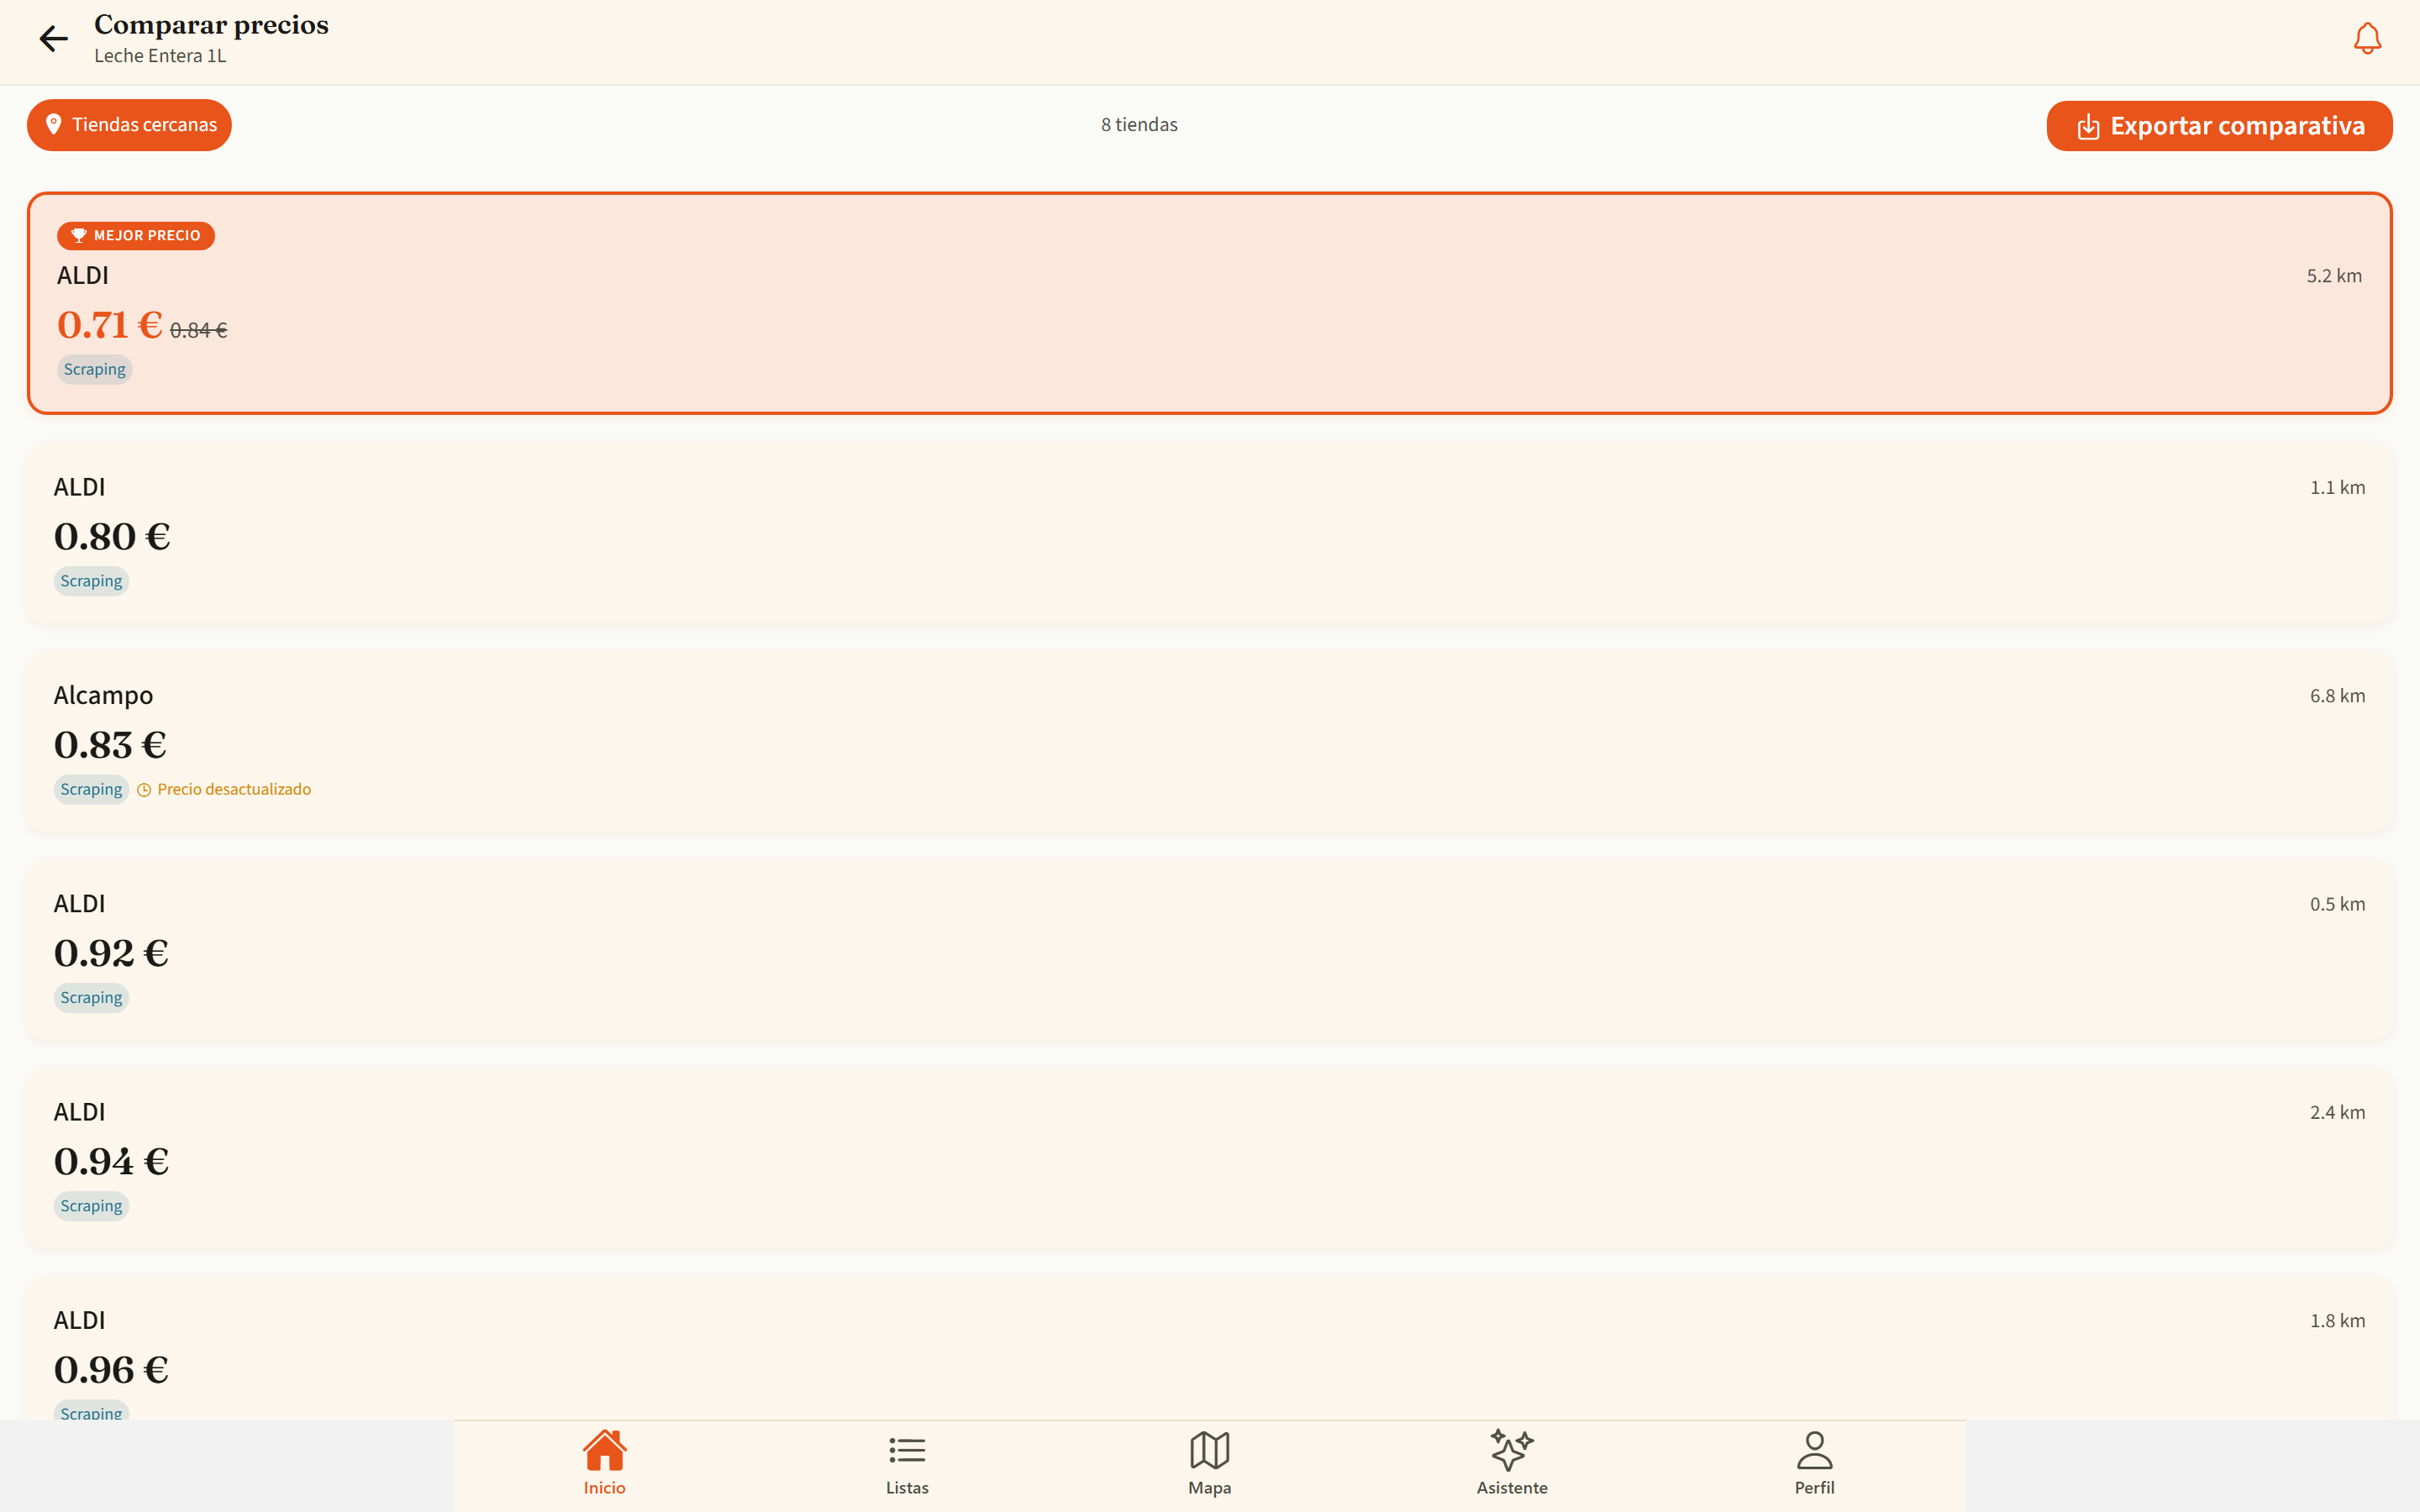
\includegraphics[width=0.48\textwidth]{diagramas/capturas/web-comparativa.png}
\hfill
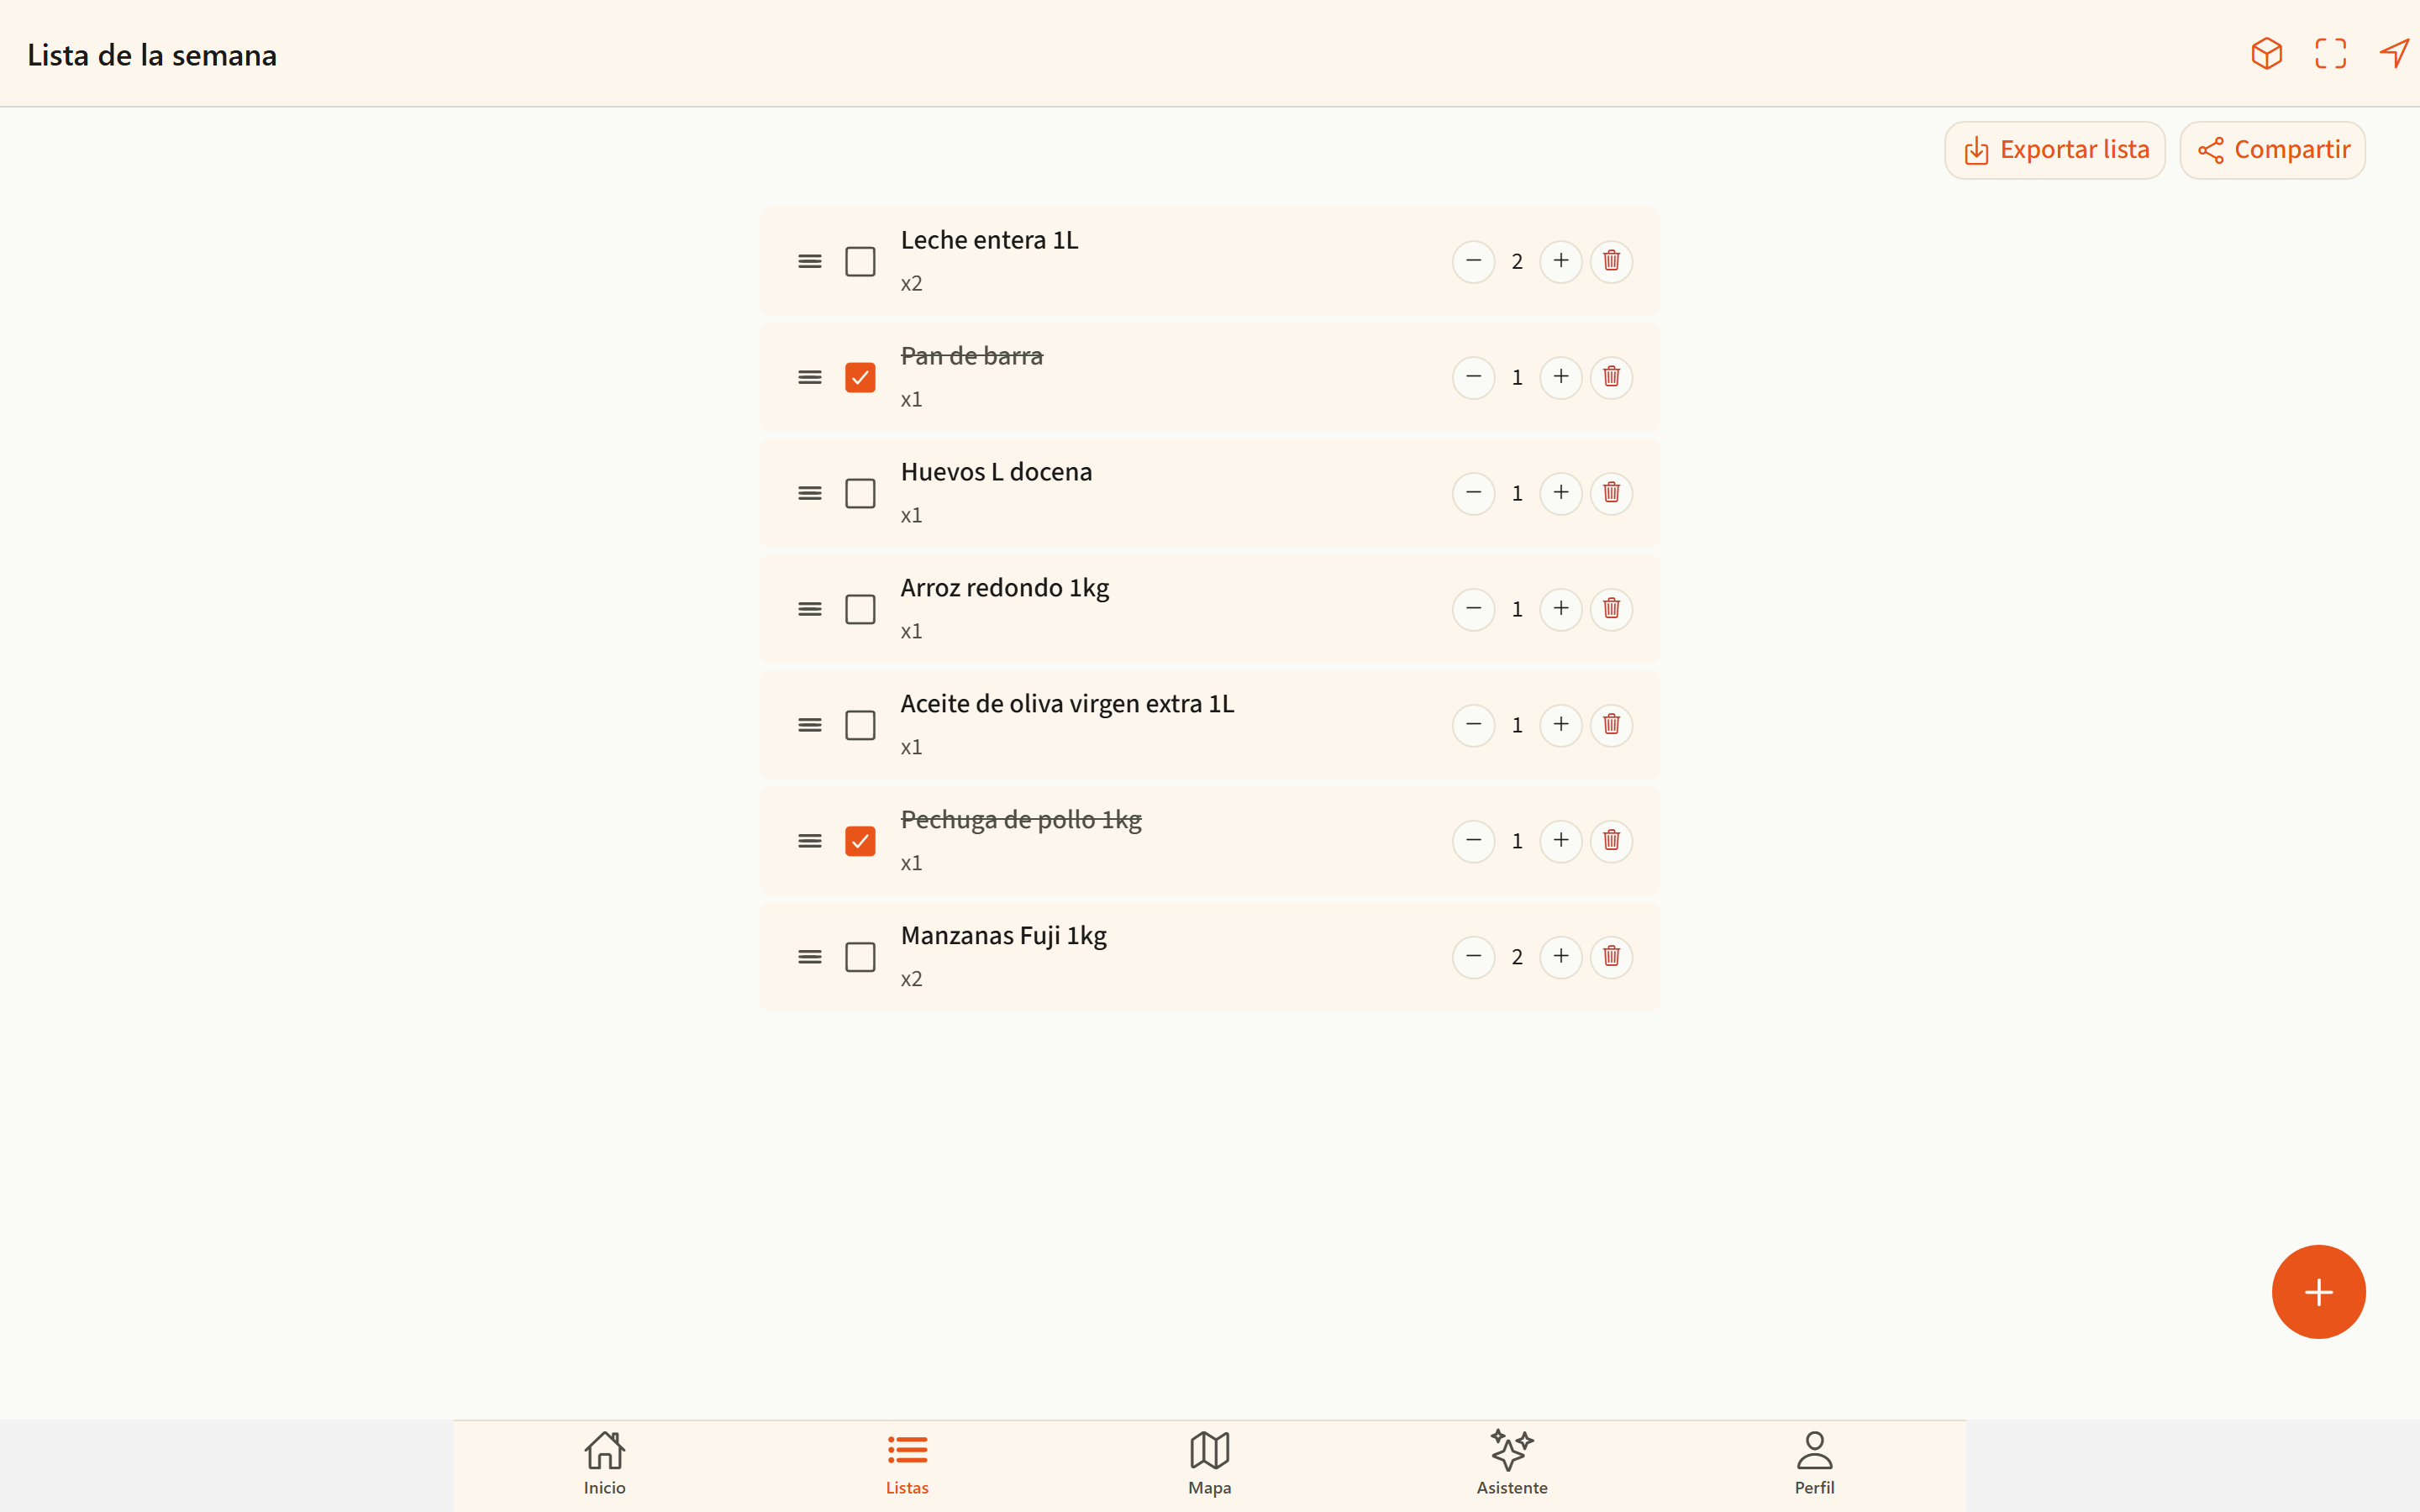
\includegraphics[width=0.48\textwidth]{diagramas/capturas/web-lista-detalle.png}
\caption{Comparativa de precios con cabecera fija y exportación CSV (izquierda) y detalle de
lista con reordenado por arrastre y exportación (derecha)}
\label{fig:manual-web-comparativa}
\end{figure}

\begin{figure}[htbp]
\centering
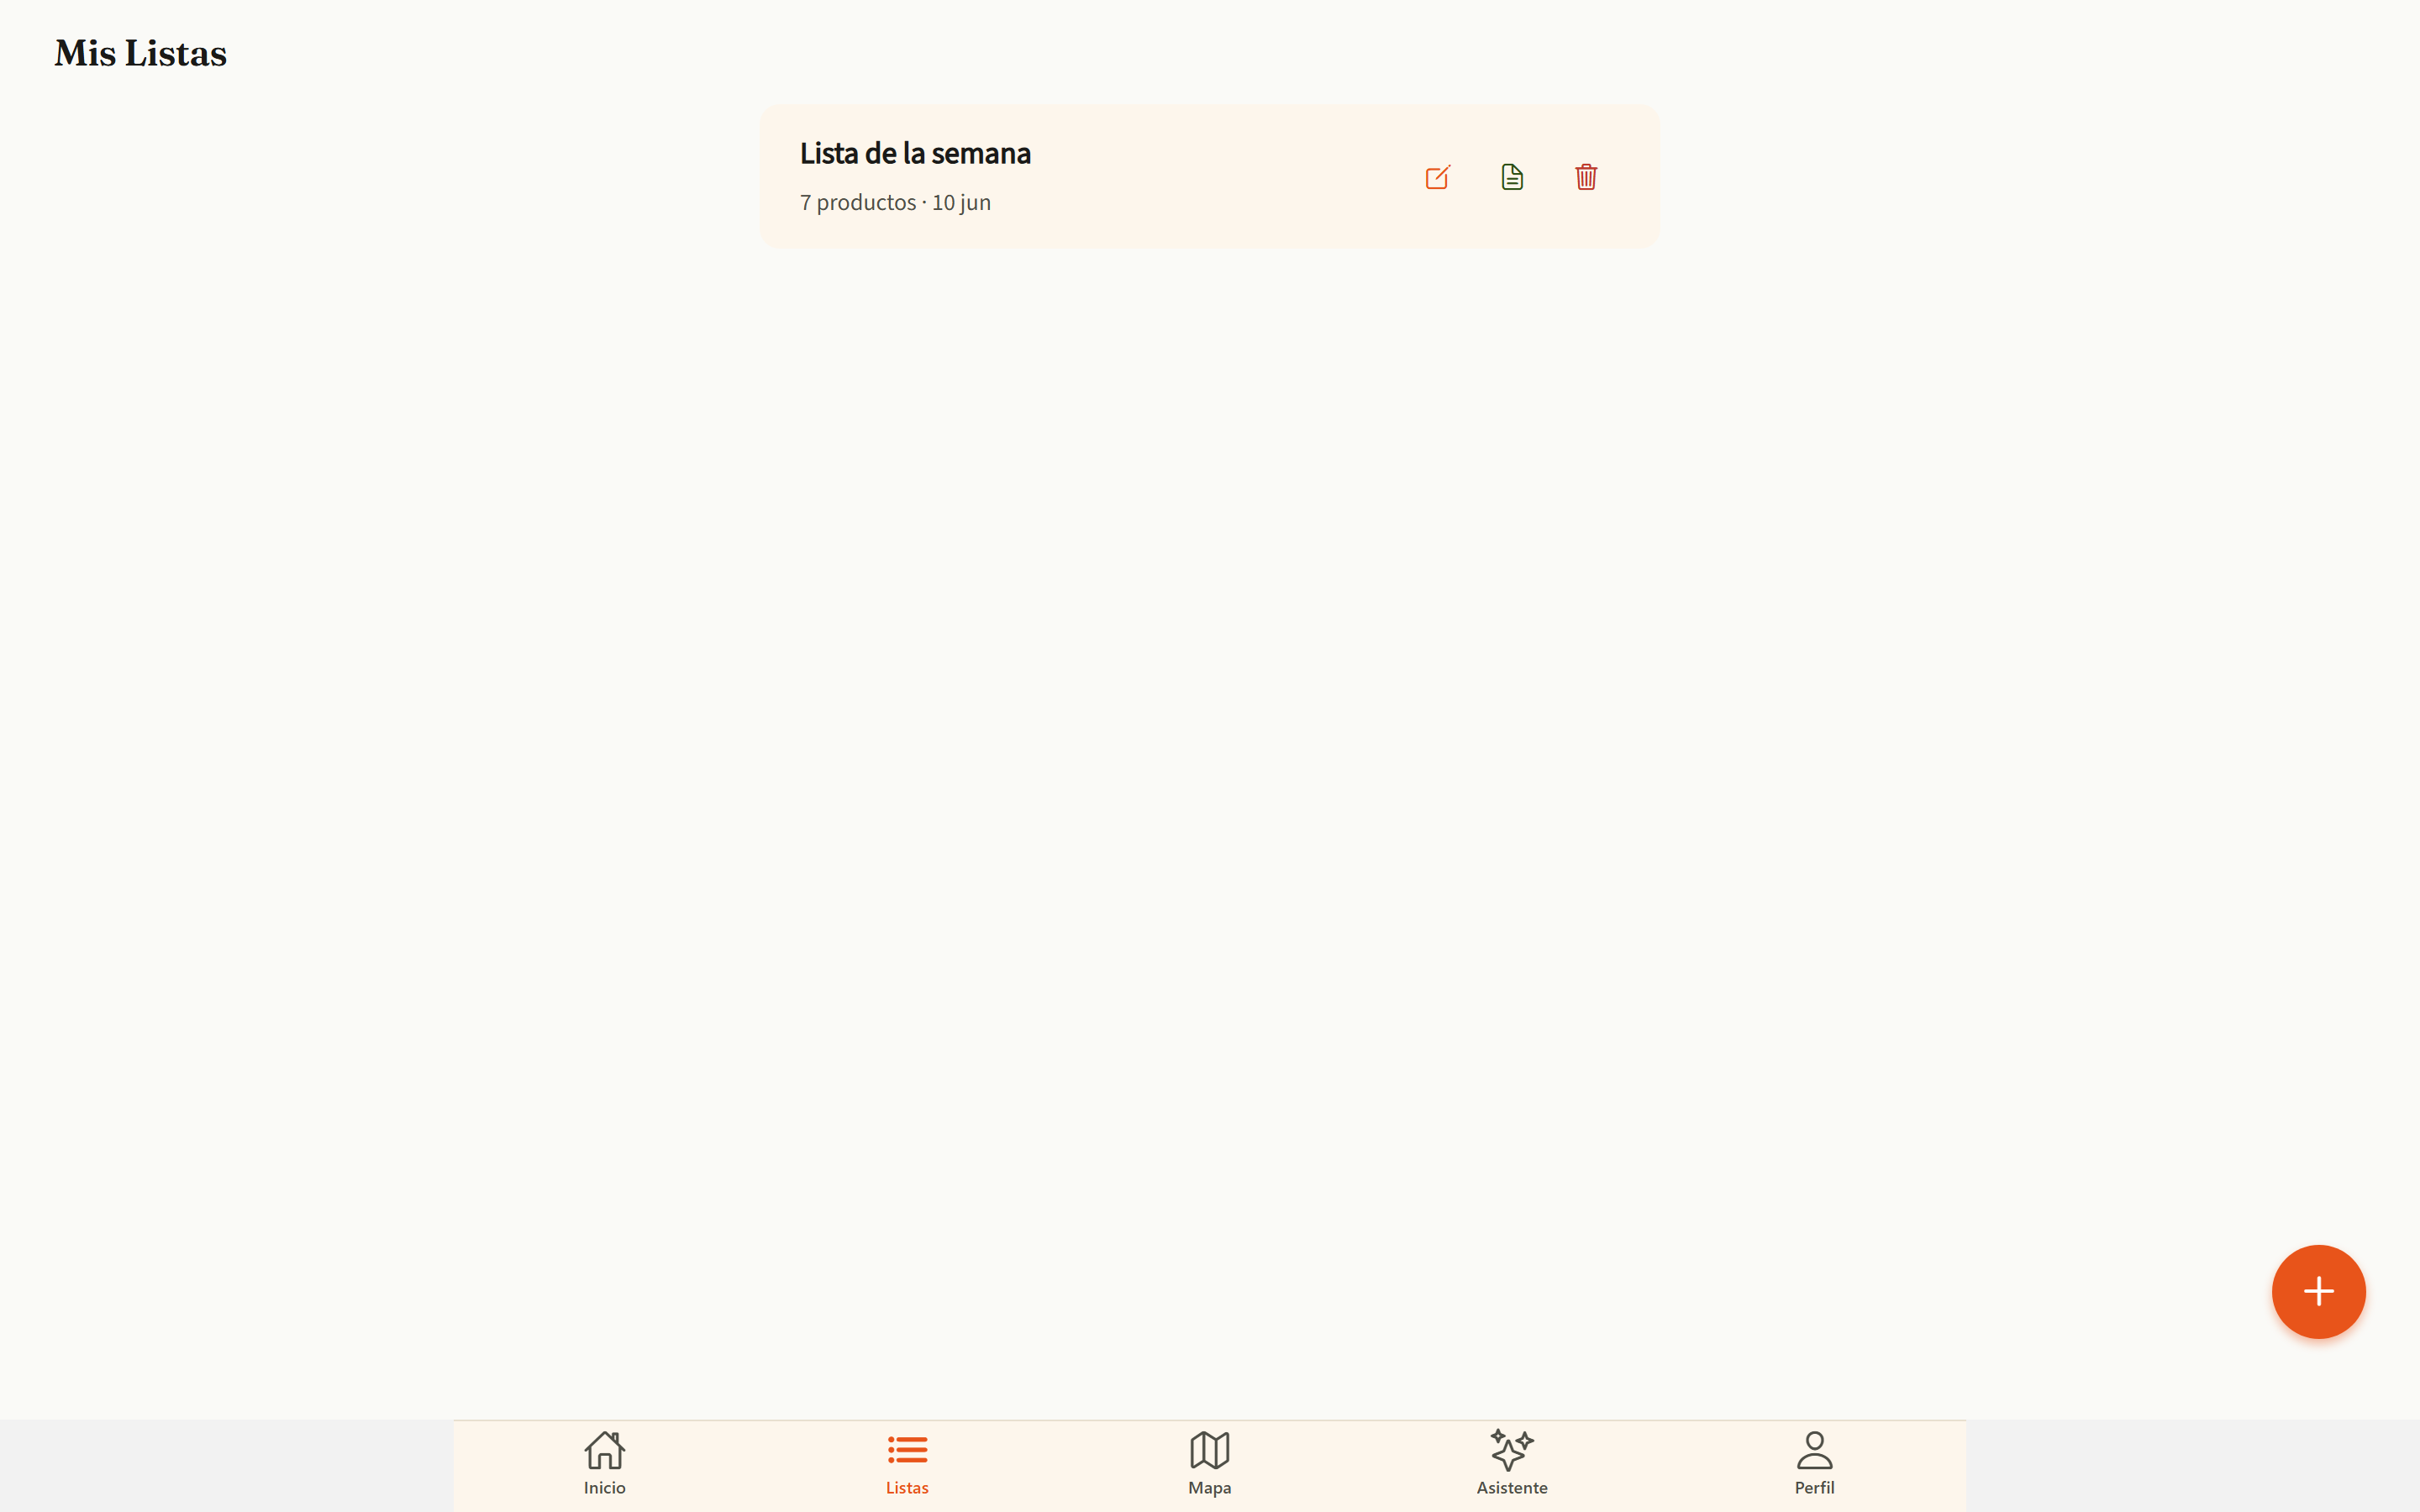
\includegraphics[width=0.48\textwidth]{diagramas/capturas/web-listas.png}
\hfill
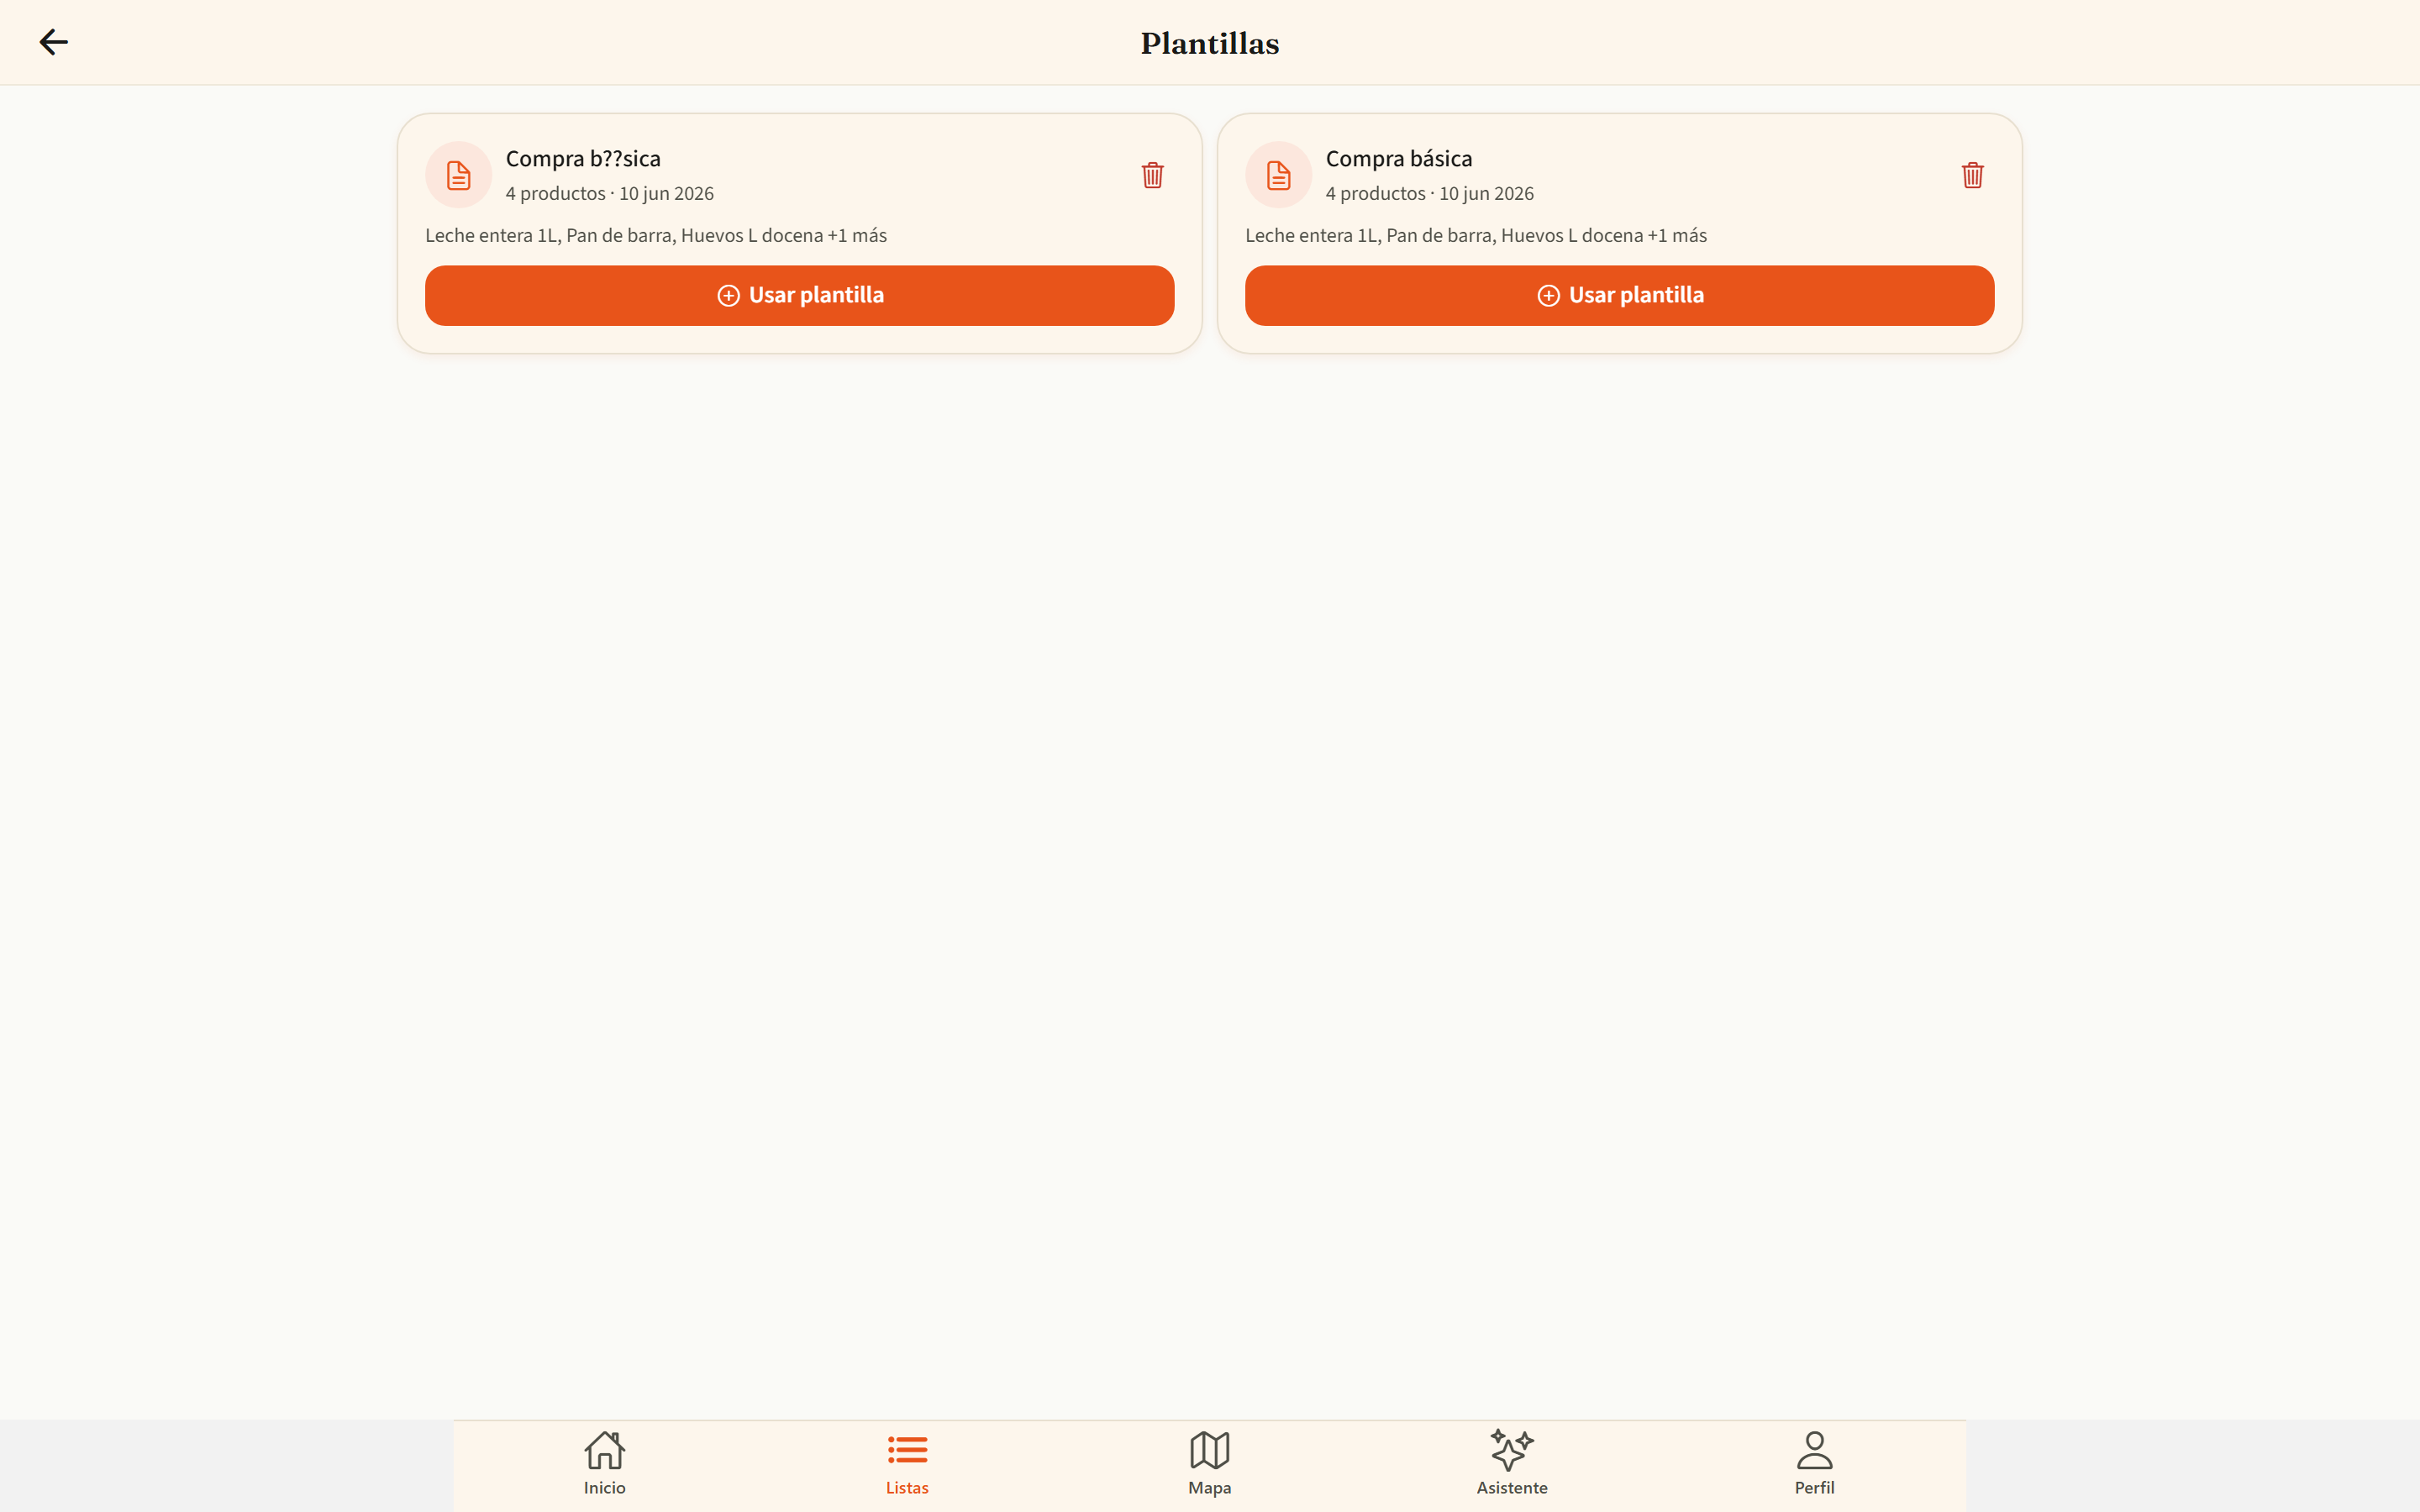
\includegraphics[width=0.48\textwidth]{diagramas/capturas/web-plantillas.png}
\caption{Colecciones en rejilla responsiva: listas de la compra (izquierda) y plantillas
(derecha)}
\label{fig:manual-web-listas}
\end{figure}

\begin{figure}[htbp]
\centering
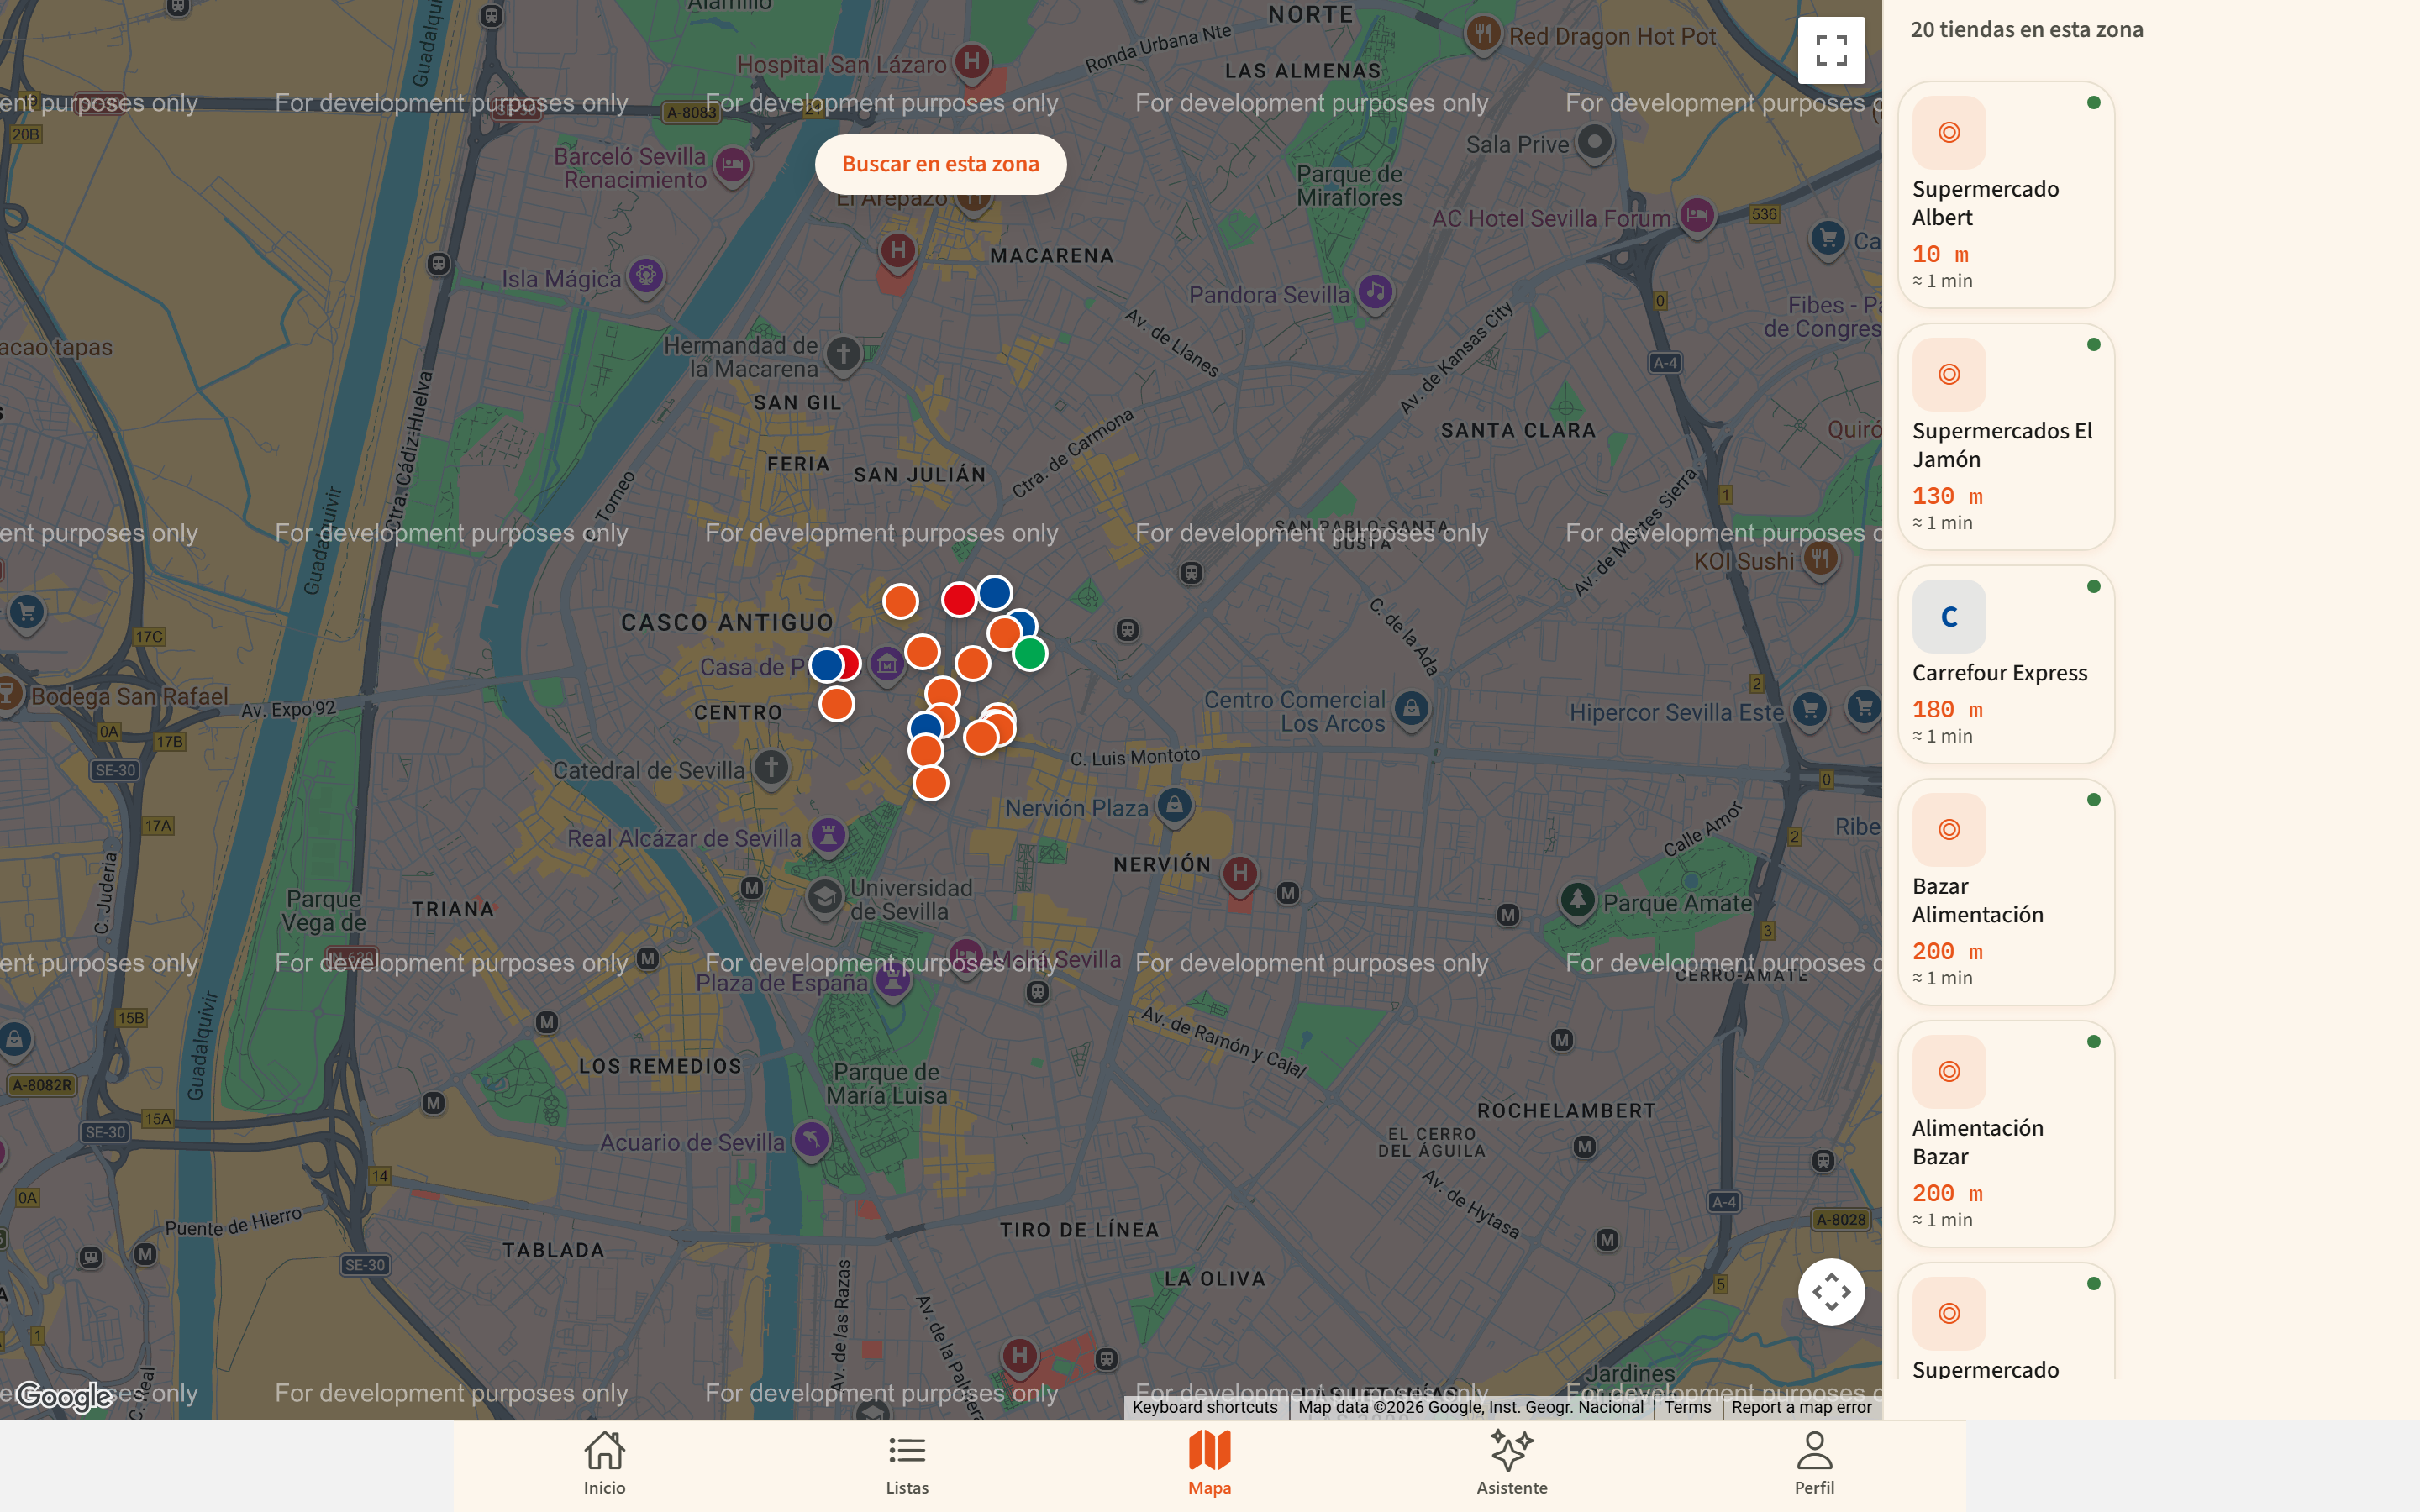
\includegraphics[width=0.48\textwidth]{diagramas/capturas/web-mapa.png}
\hfill
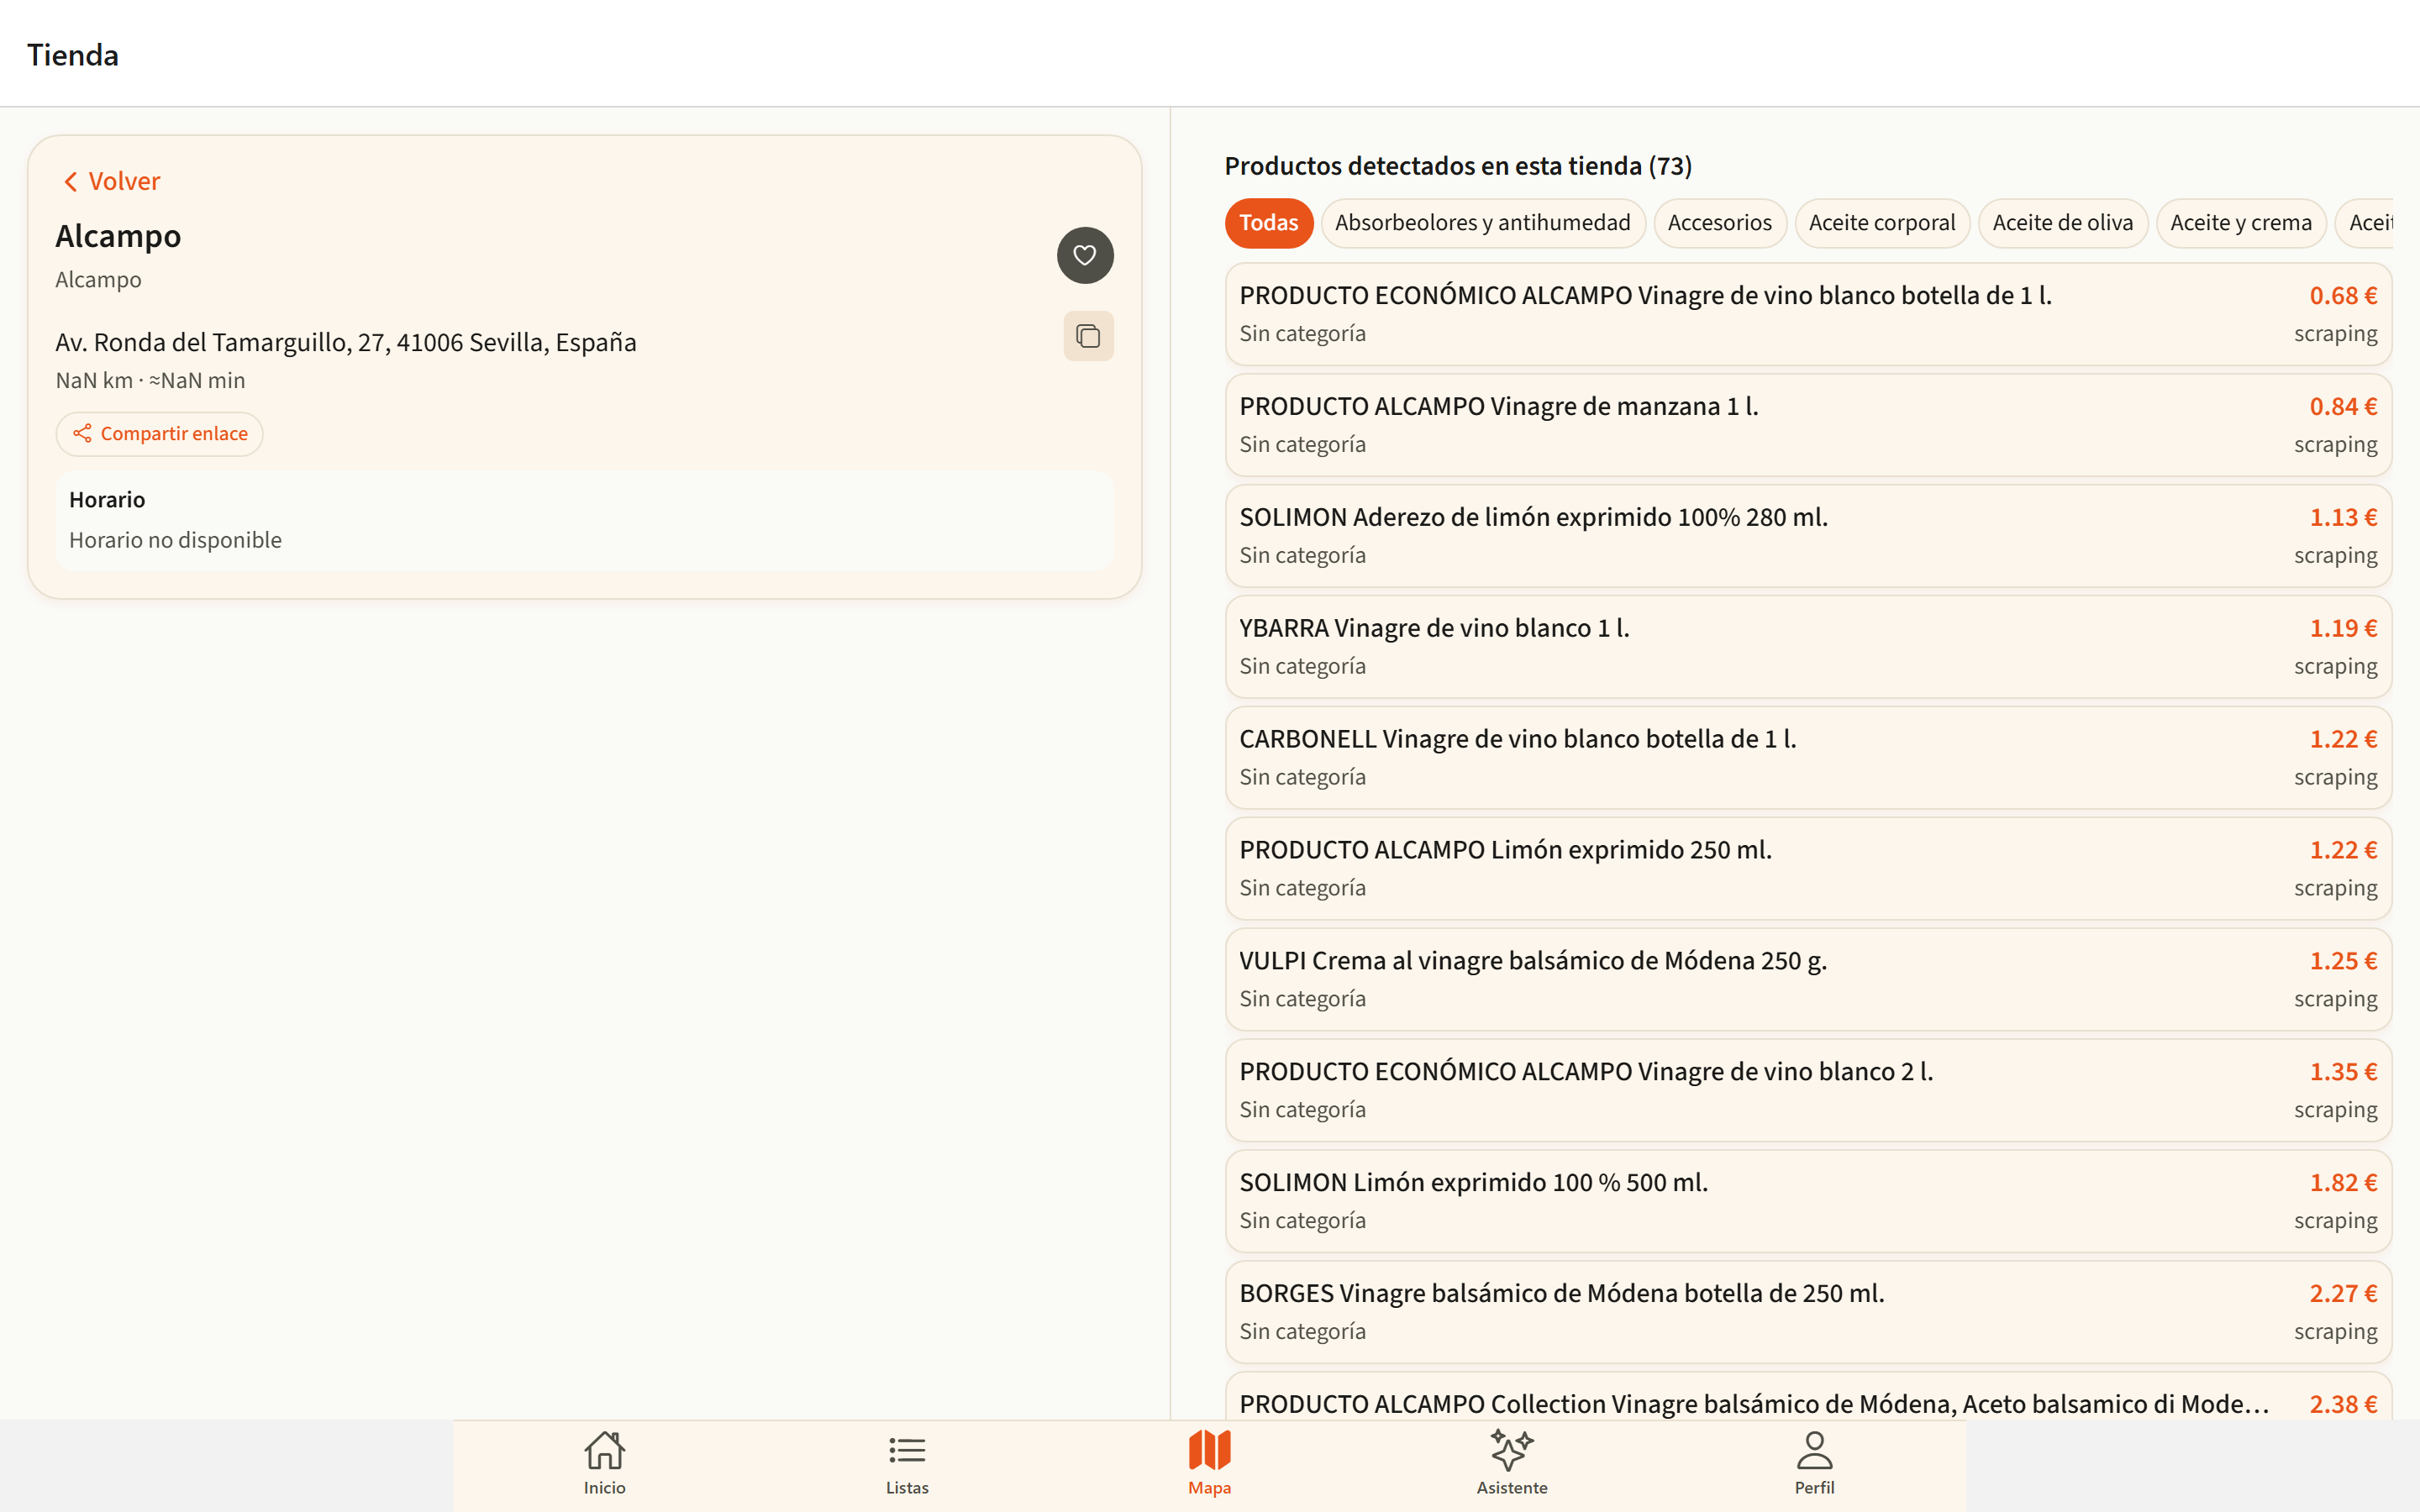
\includegraphics[width=0.48\textwidth]{diagramas/capturas/web-tienda-perfil.png}
\caption{Mapa con panel lateral de tiendas (izquierda) y perfil de tienda a dos columnas
(derecha)}
\label{fig:manual-web-mapa}
\end{figure}

\begin{figure}[htbp]
\centering
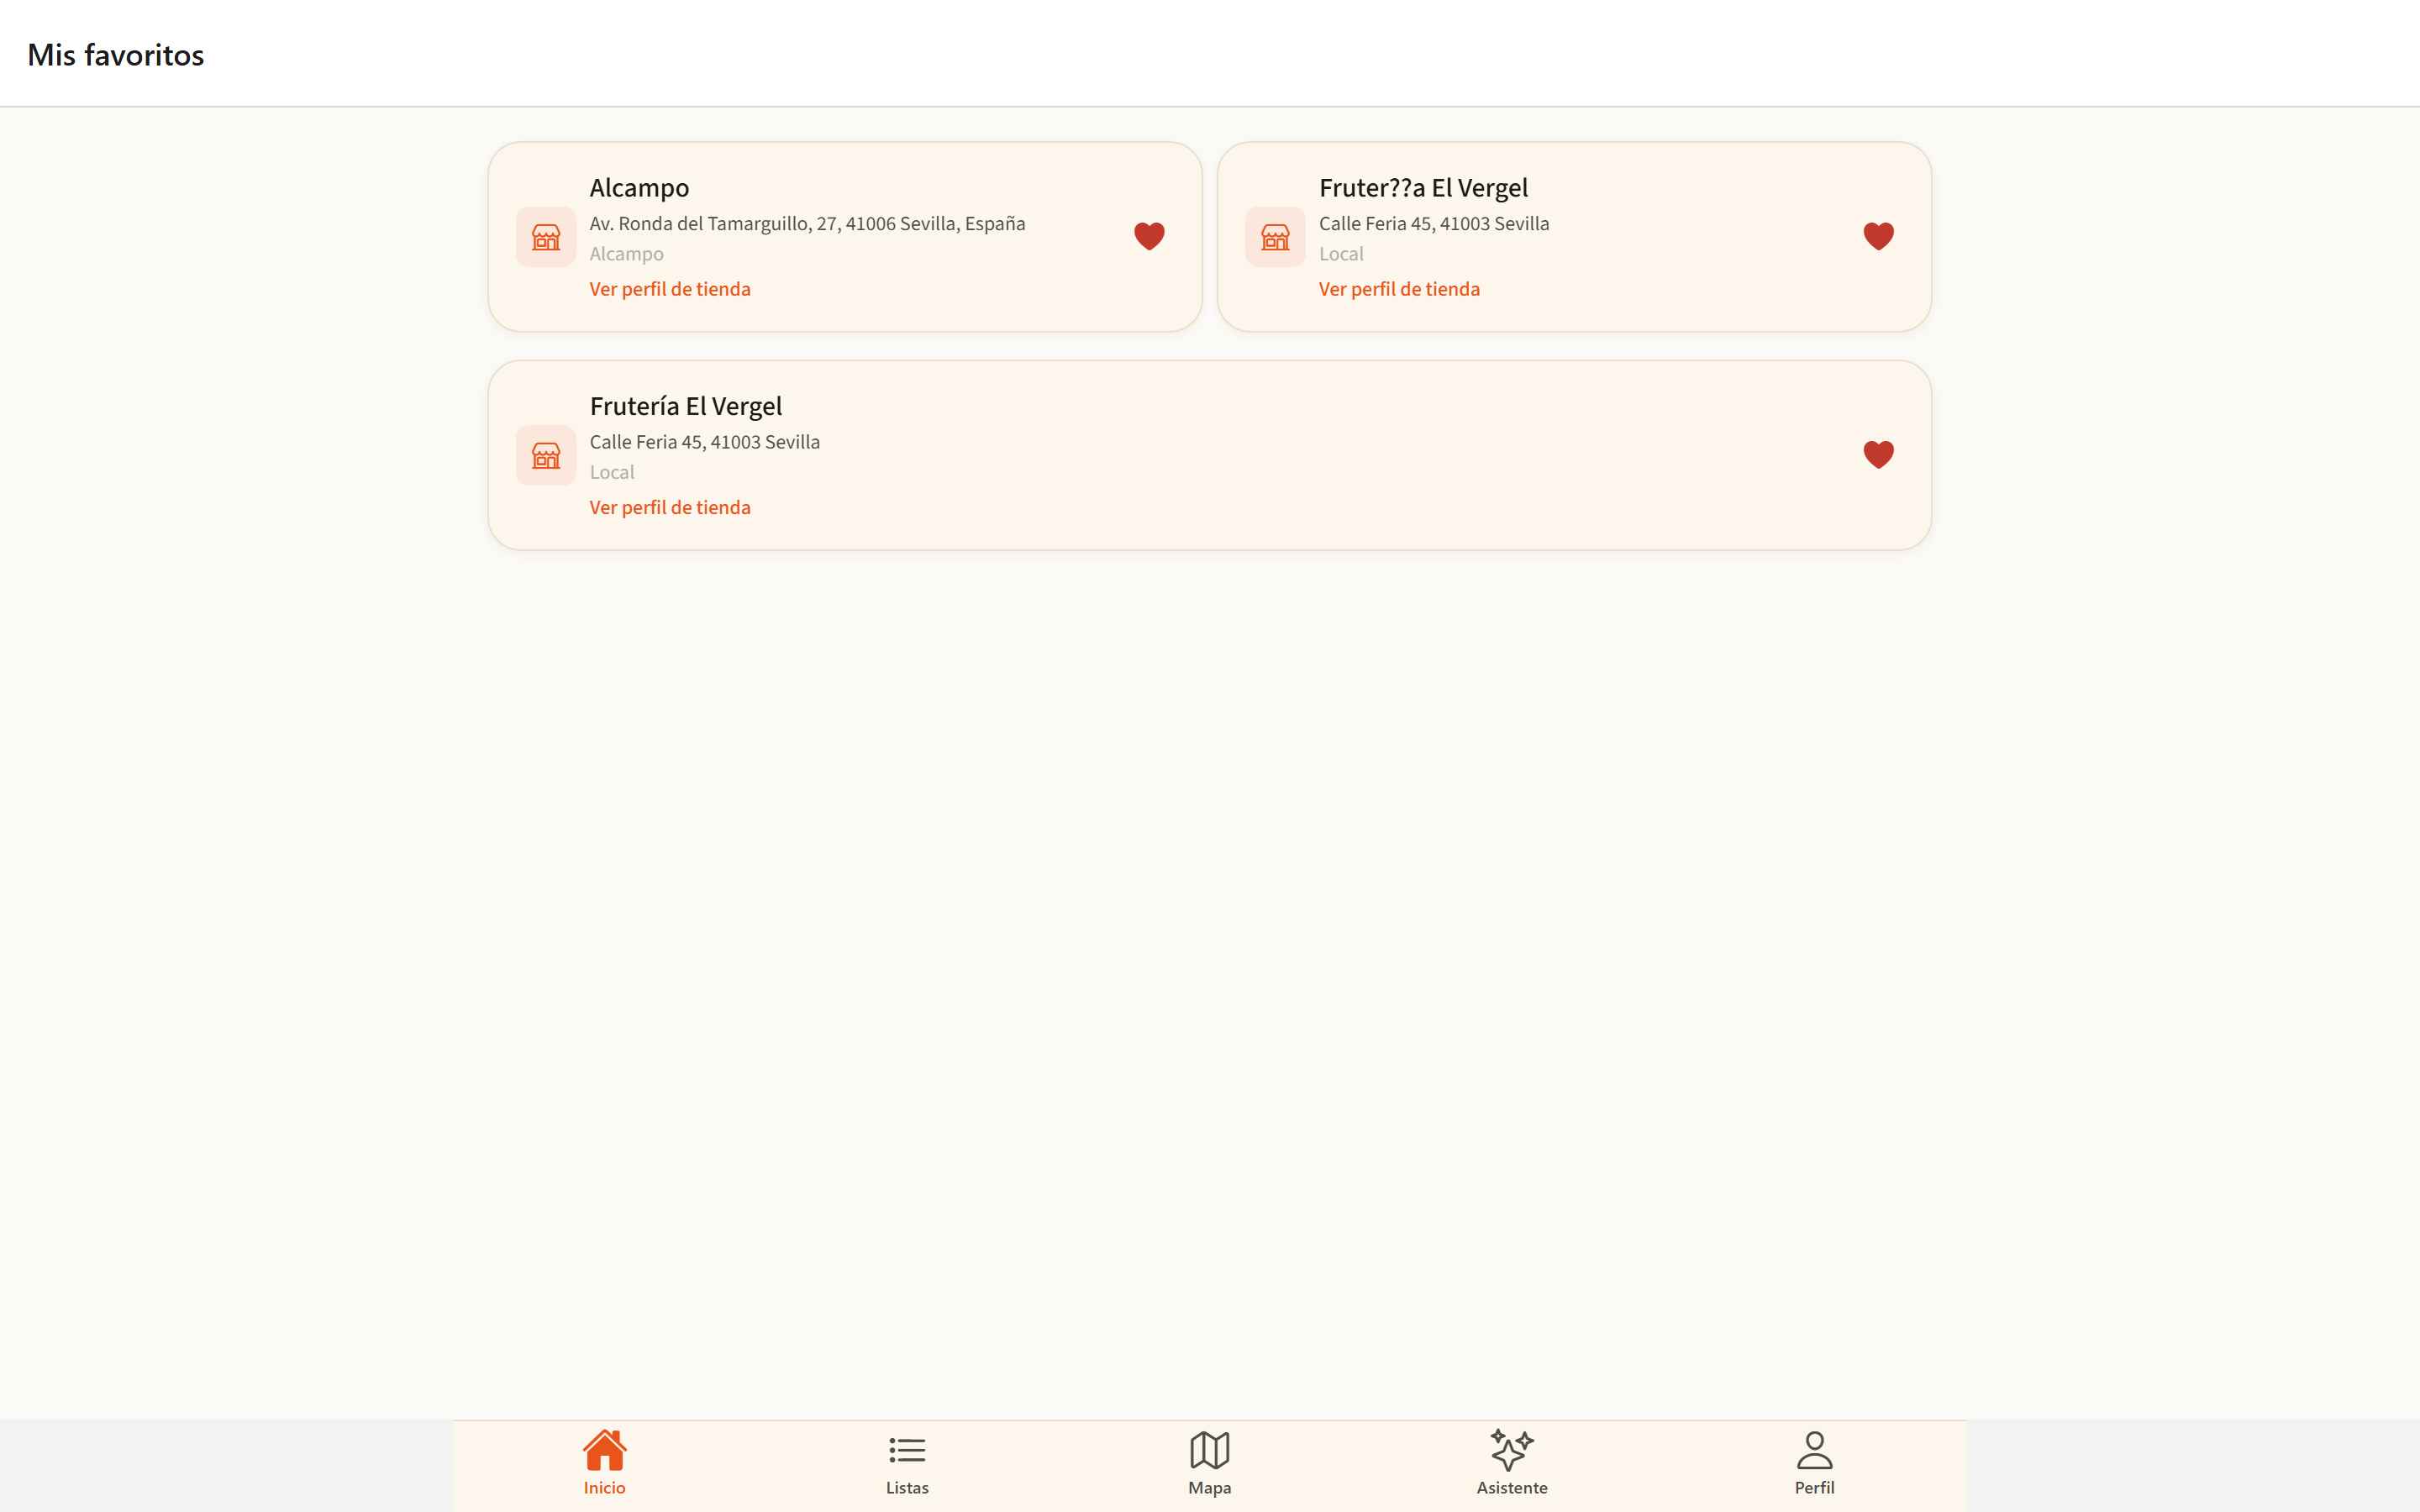
\includegraphics[width=0.48\textwidth]{diagramas/capturas/web-favoritas.png}
\hfill
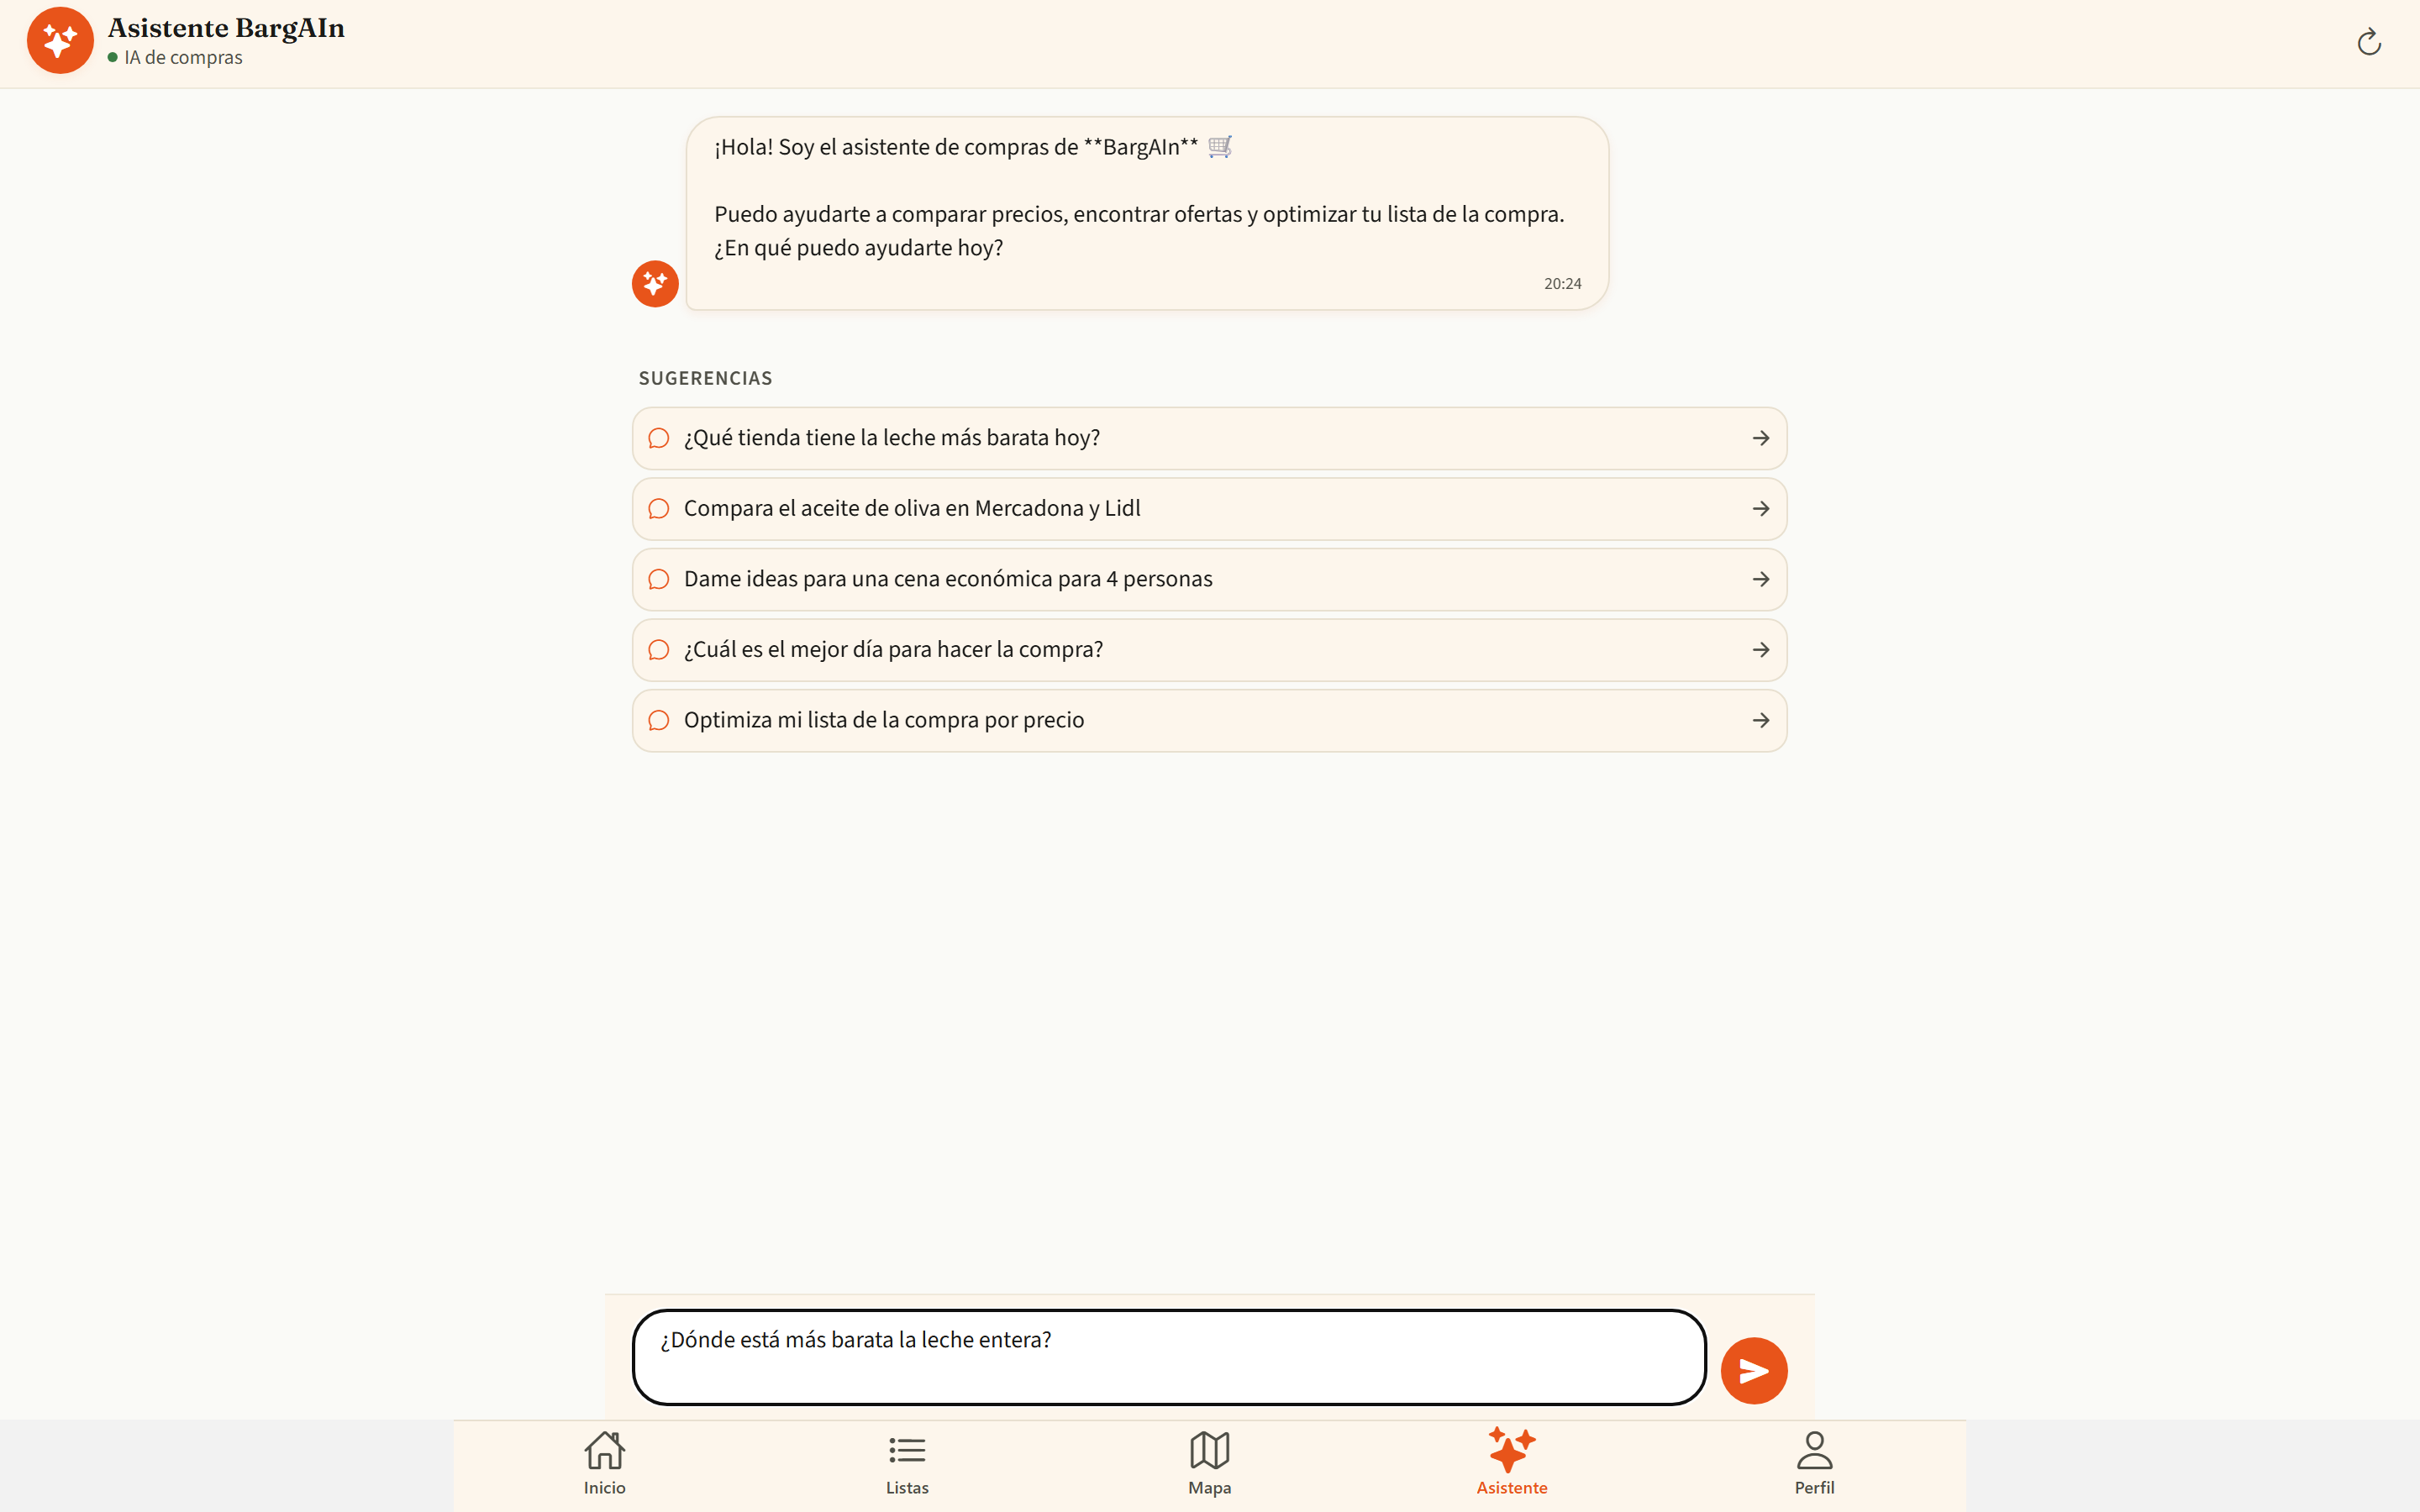
\includegraphics[width=0.48\textwidth]{diagramas/capturas/web-asistente.png}
\caption{Tiendas favoritas en rejilla (izquierda) y asistente conversacional centrado con copia
por mensaje (derecha)}
\label{fig:manual-web-favoritas}
\end{figure}

\begin{figure}[htbp]
\centering
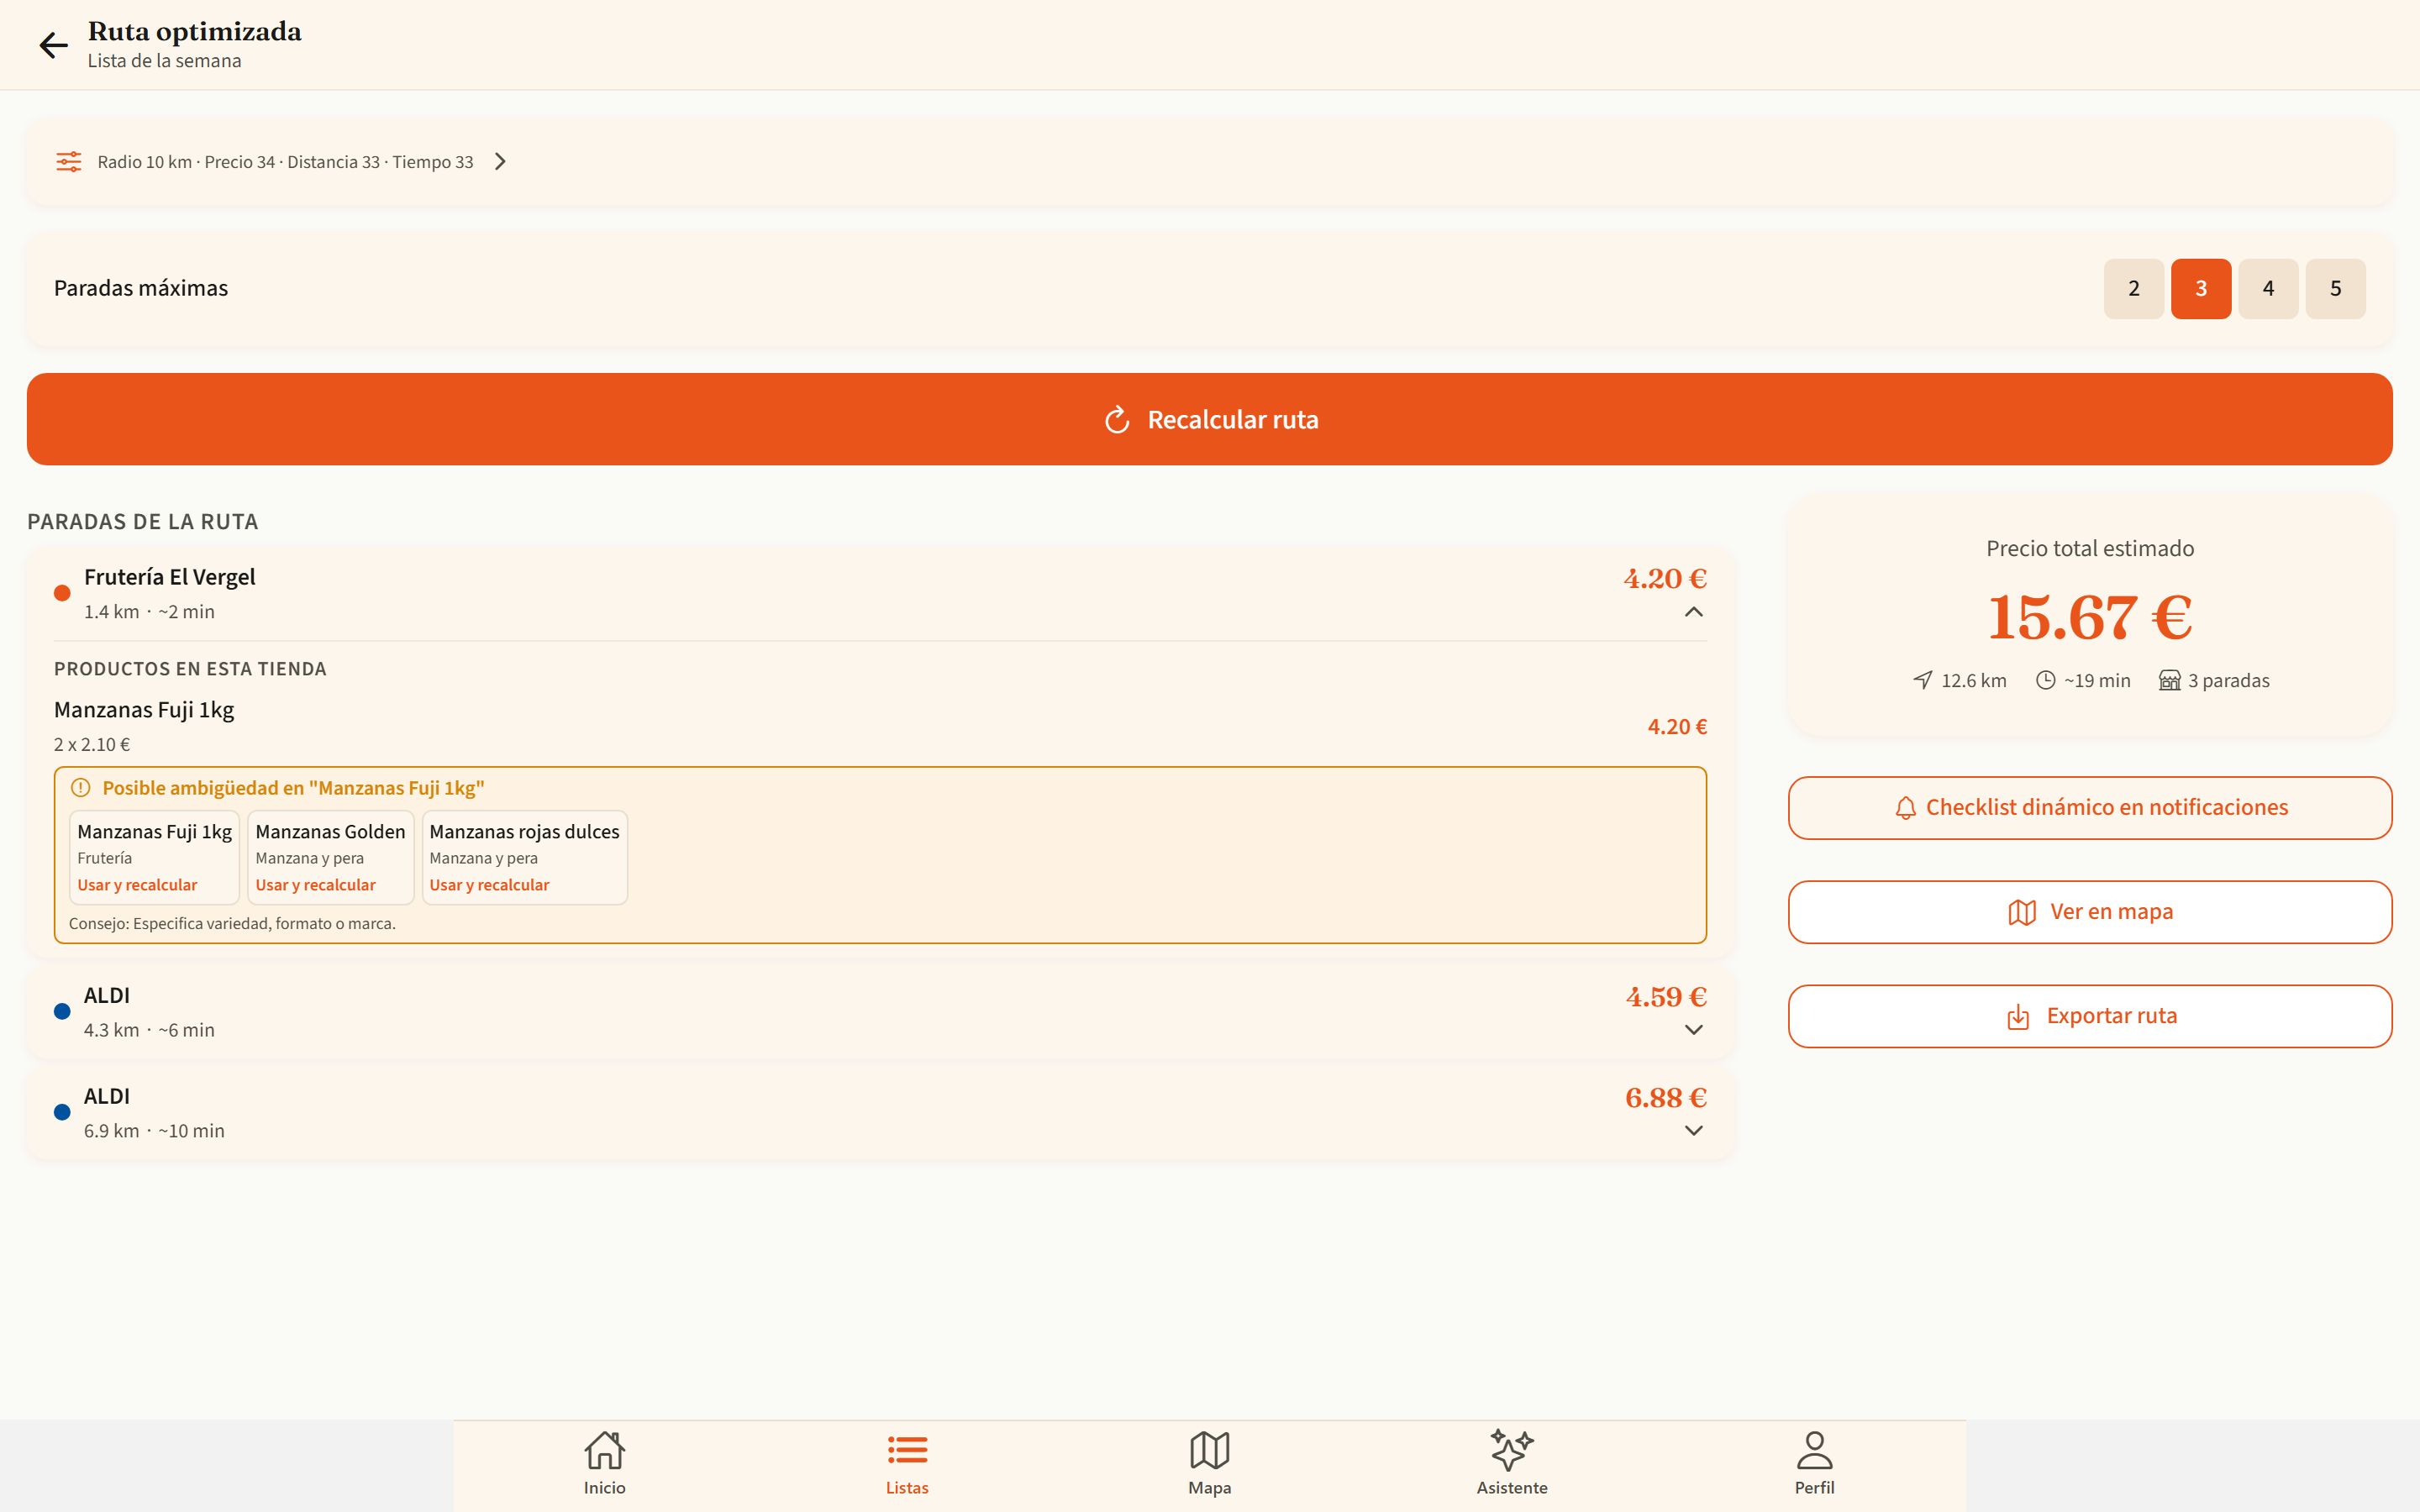
\includegraphics[width=0.48\textwidth]{diagramas/capturas/web-ruta.png}
\hfill
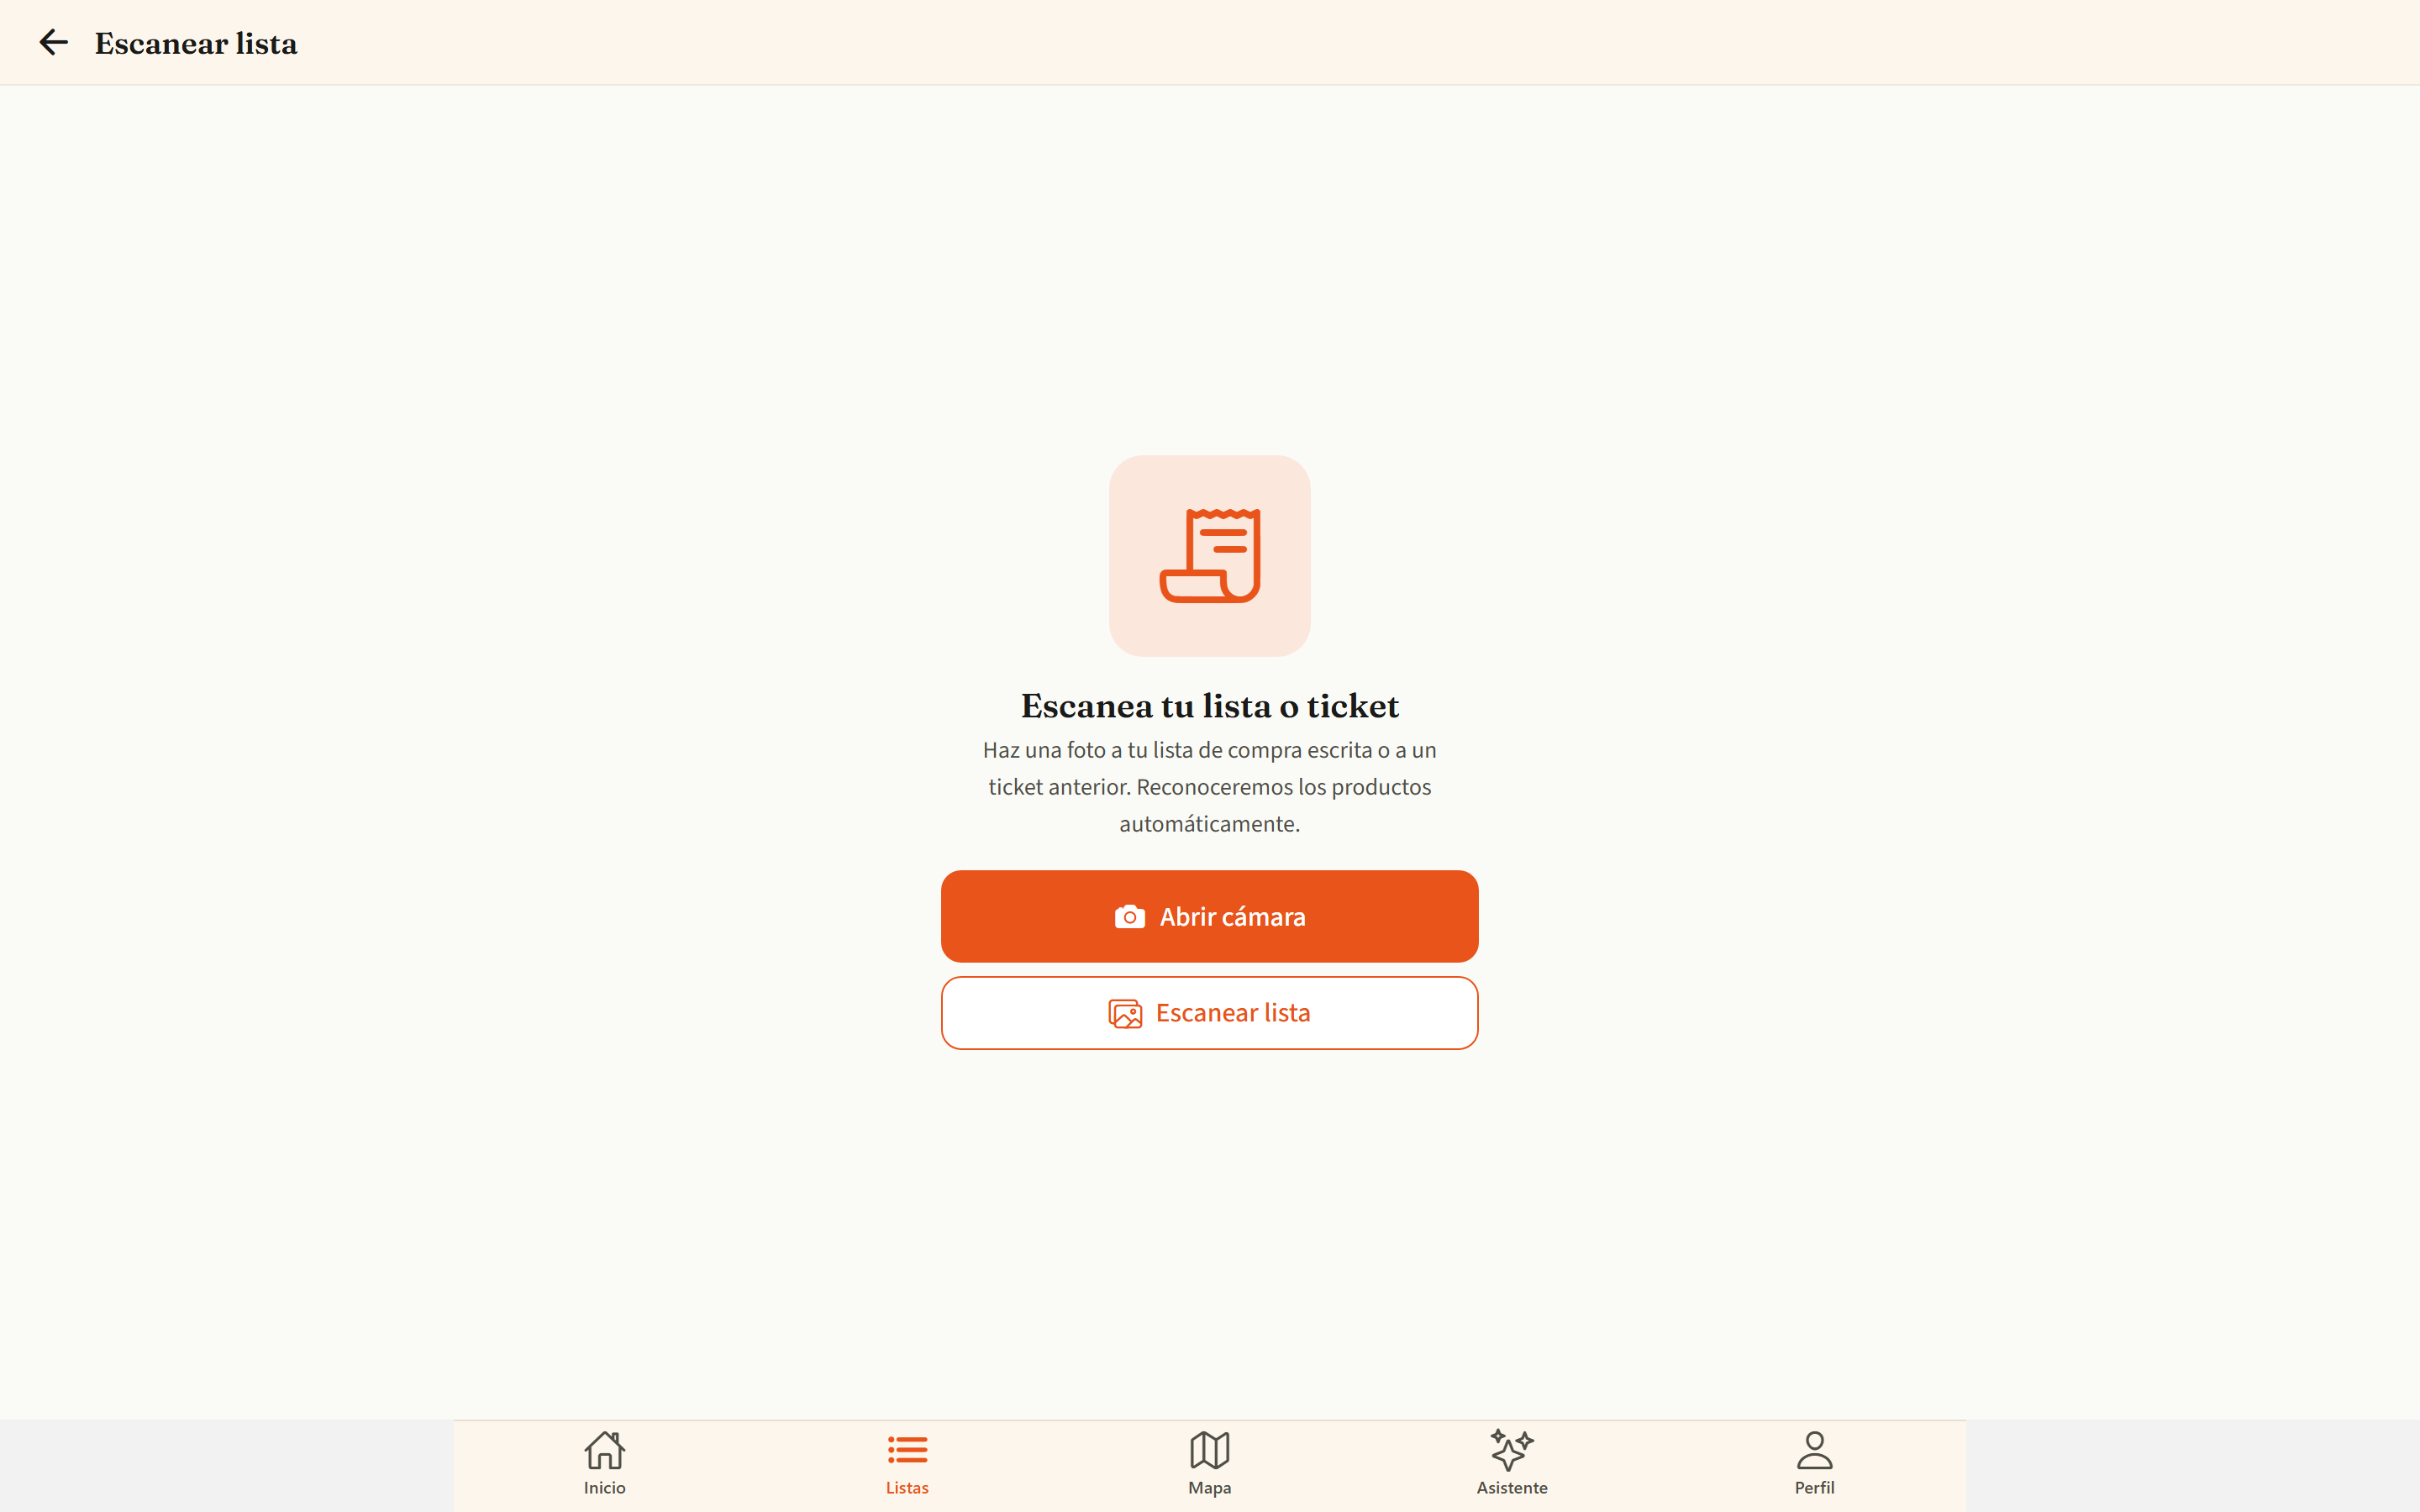
\includegraphics[width=0.48\textwidth]{diagramas/capturas/web-ocr.png}
\caption{Ruta optimizada con exportación del itinerario (izquierda) y módulo OCR adaptado al
escritorio (derecha)}
\label{fig:manual-web-ruta}
\end{figure}

\begin{figure}[htbp]
\centering
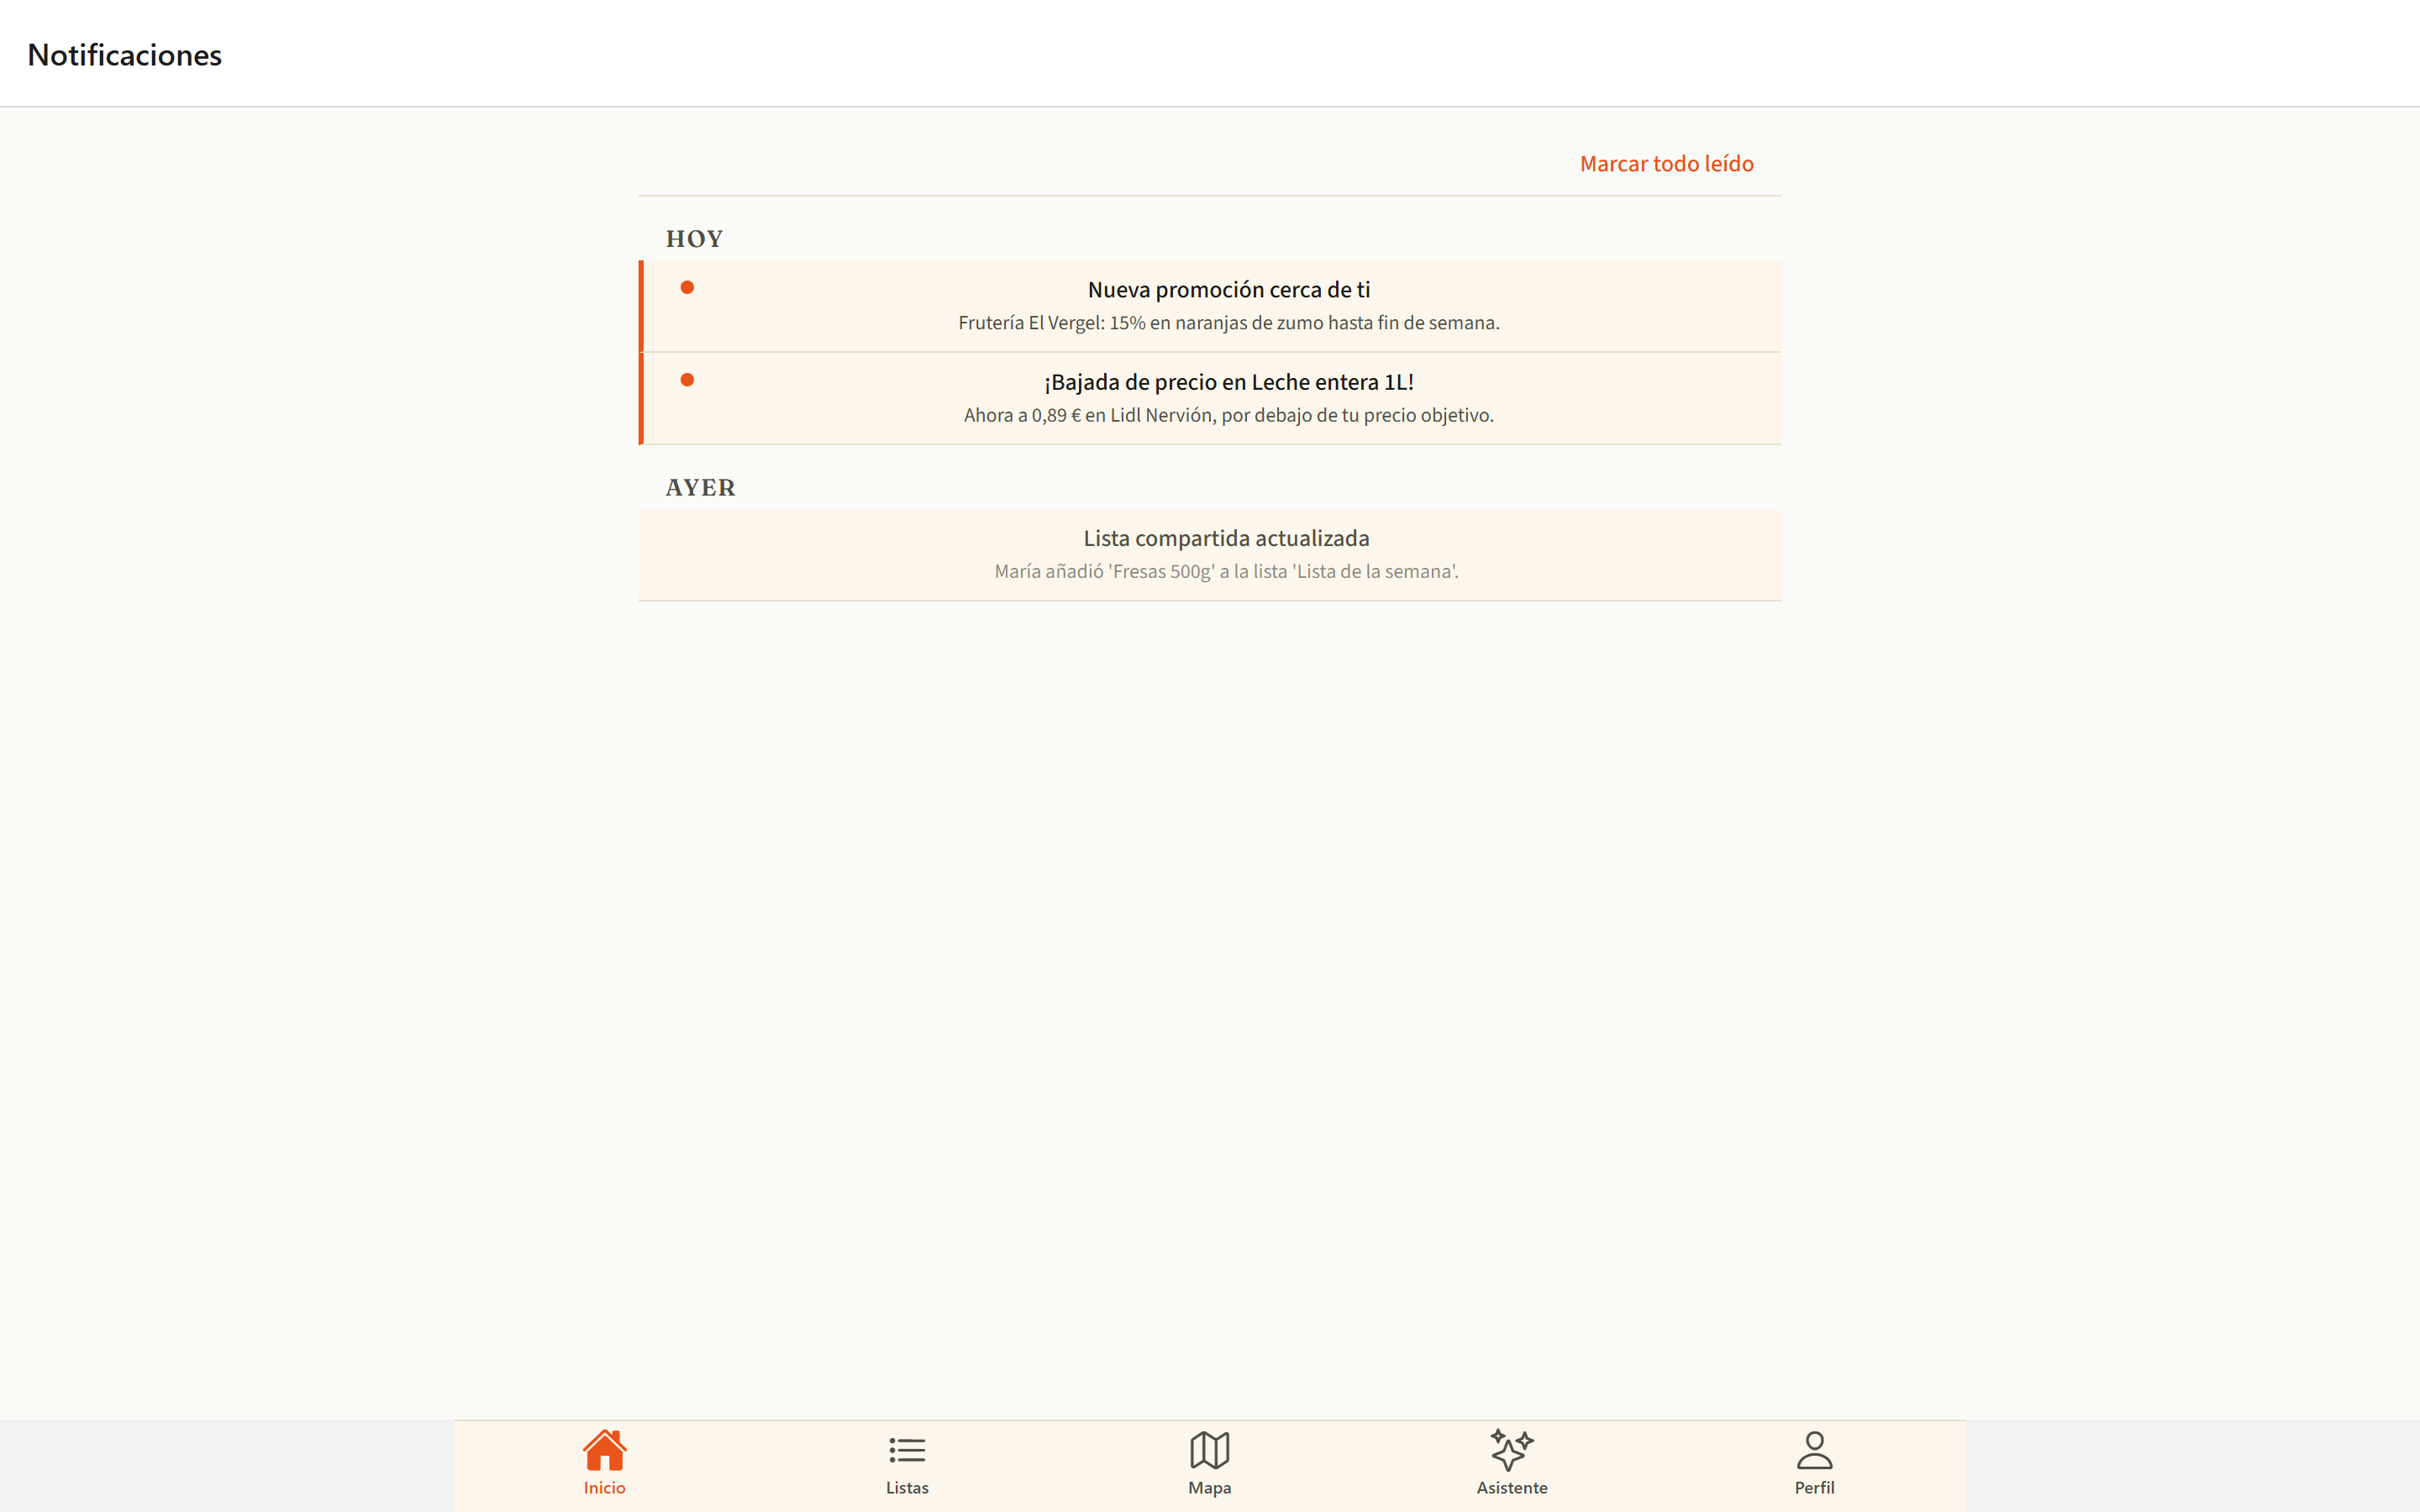
\includegraphics[width=0.48\textwidth]{diagramas/capturas/web-notificaciones.png}
\hfill
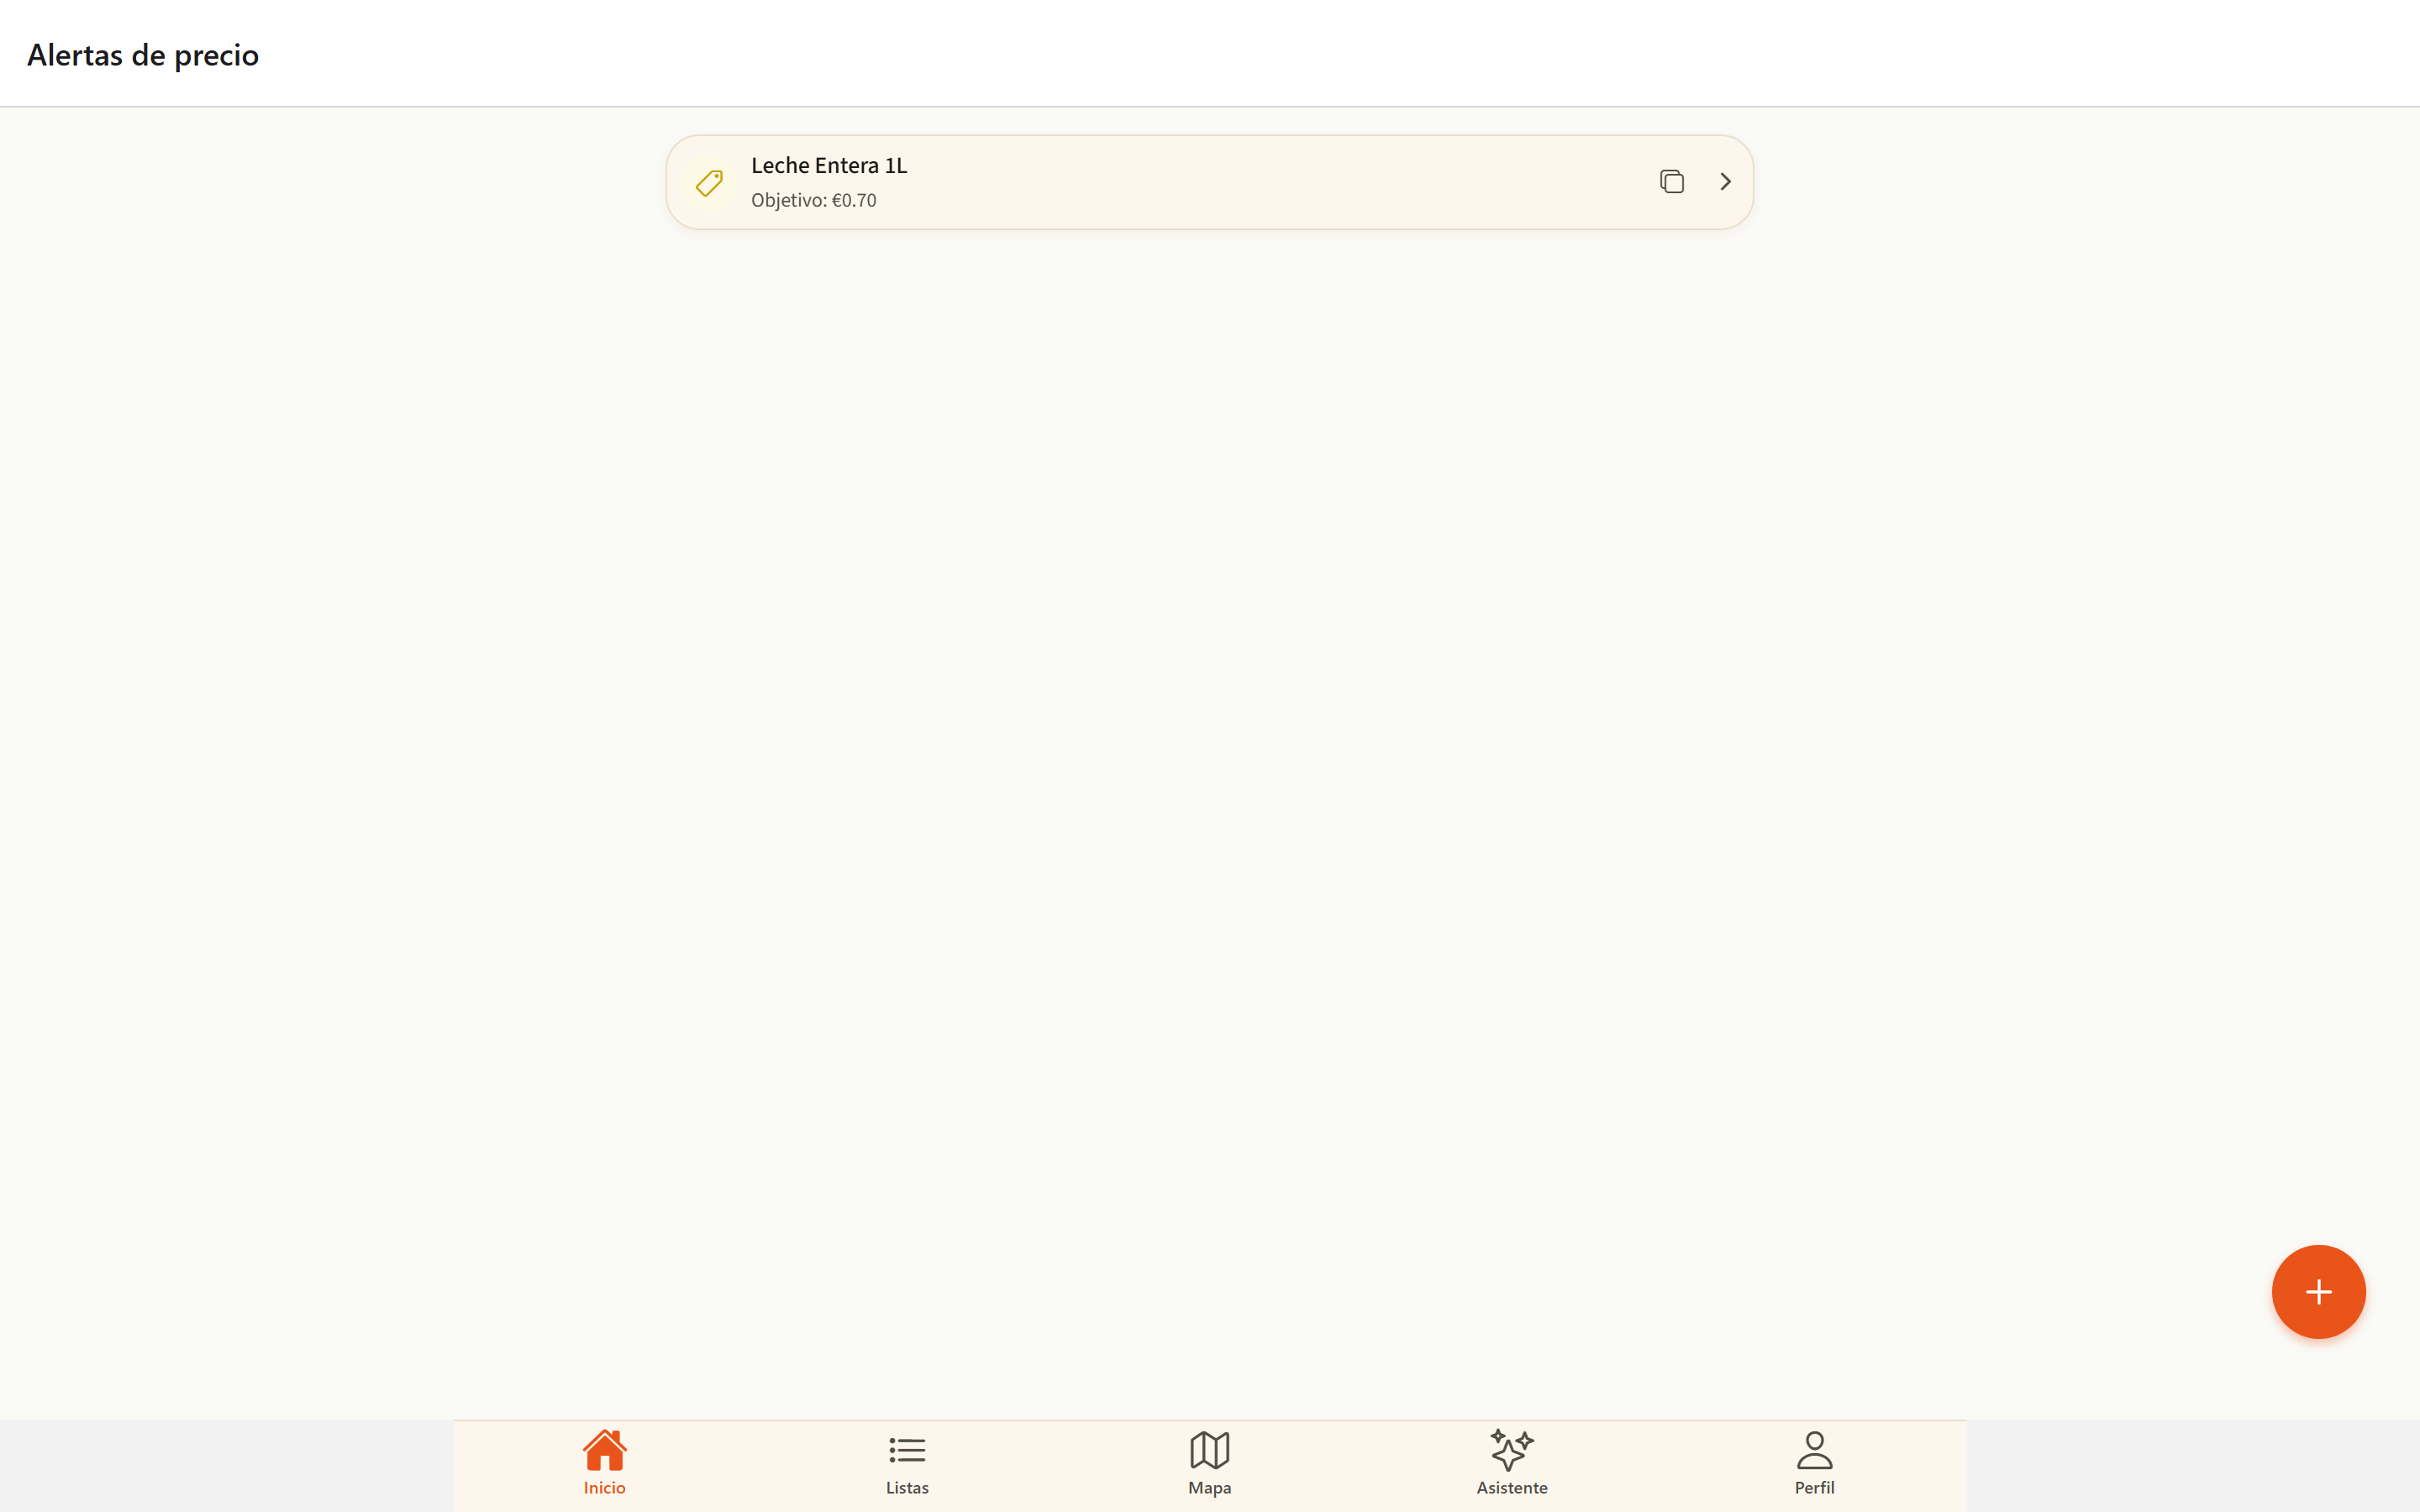
\includegraphics[width=0.48\textwidth]{diagramas/capturas/web-alertas.png}
\caption{Bandeja de notificaciones (izquierda) y alertas de precio (derecha) en la versión de
escritorio}
\label{fig:manual-web-notifs}
\end{figure}


\nocite{*}
\bibliographystyle{apacite}

\bibliography{pfcbib}

\end{document}
